% Manuscript for Behavior Research Methods, built with the Springer Nature LaTeX template (class sn-jnl with the
% APA reference style). The template files are not part of this directory; they are obtained from the publisher.
% The sections are kept in separate files while the manuscript is written and are combined into one file for
% submission. The structure and the evidence for each claim are fixed in outline.md.
% The version for submission (build.sh --submission) is double spaced, with 1-inch margins and the page number in the
% upper right corner, as the journal asks; the public version keeps the layout of the template.
\providecommand{\imsubmission}{0}
\ifnum\imsubmission=1
\documentclass[pdflatex,sn-apa,referee]{sn-jnl}
\else
\documentclass[pdflatex,sn-apa]{sn-jnl}
\fi
\ifnum\imsubmission=1
% The class loads geometry itself.
\geometry{margin=1in}
\usepackage{fancyhdr}
\pagestyle{fancy}
\fancyhf{}
\fancyhead[R]{\thepage}
\renewcommand{\headrulewidth}{0pt}
\fancypagestyle{plain}{\fancyhf{}\fancyhead[R]{\thepage}\renewcommand{\headrulewidth}{0pt}}
\fi

% T1 encoding gives the underscore of URLs and the accented letters of names their own glyphs.
\usepackage[T1]{fontenc}
\usepackage{lmodern}
% The class expects amsmath (it calls \allowdisplaybreaks at the start of the document), as in the sample article of
% the template.
\usepackage{amsmath}
\usepackage{graphicx}
\usepackage{booktabs}
\usepackage{array}

% The figures are drawn by pgfplots: Figure 1 from figures/components.tex, Figures 2 to 5 from the coordinates that
% tools/results_tables.py writes into generated/fig-*.tex with the styles below. The six colours are the first six
% slots of a categorical palette checked for separation under colour-vision deficiencies; every series also has a mark
% of its own, so that the figures can be read in grey.
\usepackage{pgfplots}
\pgfplotsset{compat=1.18}
\usepgfplotslibrary{groupplots}
\usetikzlibrary{positioning,arrows.meta,calc}
\definecolor{figc1}{HTML}{2A78D6}
\definecolor{figc2}{HTML}{EB6834}
\definecolor{figc3}{HTML}{1BAF7A}
\definecolor{figc4}{HTML}{EDA100}
\definecolor{figc5}{HTML}{E87BA4}
\definecolor{figc6}{HTML}{008300}
\pgfplotsset{
  fig panel/.style={tick label style={font=\footnotesize}, title style={font=\footnotesize},
    label style={font=\footnotesize}, legend style={font=\footnotesize, draw=none}, legend cell align=left,
    ymajorgrids, major grid style={black!12}, scaled y ticks=false,
    y tick label style={/pgf/number format/fixed, /pgf/number format/1000 sep={{,}}}},
  fig proportion/.style={ymin=-0.03, ymax=1.03, ytick={0,0.25,0.5,0.75,1}},
  fig zero/.style={extra y ticks={0}, extra y tick labels={}, extra y tick style={grid=major,
    major grid style={black!60, dashed}}},
  fig slow/.style={color=figc1, mark=*},
  fig mid/.style={color=figc2, mark=square*},
  fig fast/.style={color=figc3, mark=triangle*},
  fig set1/.style={color=figc1, mark=*},
  fig set2/.style={color=figc2, mark=square*},
  fig set3/.style={color=figc3, mark=triangle*},
  fig set4/.style={color=figc4, mark=diamond*},
  fig set5/.style={color=figc5, mark=pentagon*},
  fig set6/.style={color=figc6, mark=star, mark options={line width=0.8pt}},
  fig point/.style={only marks, mark size=1.5pt},
  fig open/.style={mark options={fill=white, line width=0.4pt}},
  fig limit/.style={only marks, mark=-, mark size=3pt, mark options={line width=1pt}},
  fig interval/.style={no markers, line width=0.6pt, unbounded coords=jump},
  fig chance/.style={no markers, black!70, samples=2},
  fig margin/.style={no markers, black!70, dashed, samples=2},
}

% A ragged-right paragraph column whose width, given as a fraction of the line, includes the space between columns, so
% that columns whose fractions sum to at most one fit the line.
\newcolumntype{L}[1]{>{\raggedright\arraybackslash}p{\dimexpr#1\linewidth-2\tabcolsep\relax}}

% The APA style of the template prints the url field of a reference as plain text, so an underscore in a URL stops the
% compilation; the environment that holds the field is redefined to pass the URL to \url.
\makeatletter
\AtBeginDocument{%
  \renewenvironment{APACrefURL}[1][]{%
    \ifx\@empty#1\@empty\BRetrievedFrom\else\BRetrieved{#1}\fi\url}{}}
\makeatother

% Bookmarks go down to subsections; the run-in paragraph headings are not bookmarked.
\hypersetup{bookmarksdepth=2}

% A value that is filled in from the result files or the run manifests after the measurement.
\newcommand{\tbd}[1]{\textbf{[#1]}}

% A value of the results, generated from the result files by tools/results_tables.py into generated/values.tex; a key
% without a generated value prints as a value still to be filled in and is reported in the log, where build.sh counts
% it.
\newcommand{\rv}[1]{\ifcsname rv:#1\endcsname\csname rv:#1\endcsname\else\tbd{#1}%
  \PackageWarningNoLine{results}{Result value #1 not generated}\fi}
% Generated by manuscript/tools/results_tables.py from the result files; do not edit by hand.
% Read with \rv{<key>}; the source of each value is in values.json.
\expandafter\def\csname rv:macos-standard-live-off.abandon.continued.unknown.all\endcsname{0}
\expandafter\def\csname rv:macos-standard-live-off.abandon.continued.unknown.primary\endcsname{0}
\expandafter\def\csname rv:macos-standard-live-off.abandon.continued.with.all\endcsname{-- (0 pairs)}
\expandafter\def\csname rv:macos-standard-live-off.abandon.continued.with.primary\endcsname{-- (0 pairs)}
\expandafter\def\csname rv:macos-standard-live-off.abandon.continued.without.all\endcsname{0.979 [0.972, 0.985] (2{,}016 pairs)}
\expandafter\def\csname rv:macos-standard-live-off.abandon.continued.without.primary\endcsname{0.979 [0.971, 0.984] (1{,}981 pairs)}
\expandafter\def\csname rv:macos-standard-live-off.all.dwellbias.range\endcsname{$-$739 to 201~ms}
\expandafter\def\csname rv:macos-standard-live-off.all.dwellbias.speeds.left\endcsname{0}
\expandafter\def\csname rv:macos-standard-live-off.all.dwellbias.speeds.used\endcsname{3}
\expandafter\def\csname rv:macos-standard-live-off.all.precision.range\endcsname{0.000--1.000}
\expandafter\def\csname rv:macos-standard-live-off.all.precision.strata.left\endcsname{2}
\expandafter\def\csname rv:macos-standard-live-off.all.precision.strata.leftnames\endcsname{S13 (slow, fast)}
\expandafter\def\csname rv:macos-standard-live-off.all.precision.strata.used\endcsname{37}
\expandafter\def\csname rv:macos-standard-live-off.all.recall.range\endcsname{0.000--1.000}
\expandafter\def\csname rv:macos-standard-live-off.all.recall.strata.left\endcsname{0}
\expandafter\def\csname rv:macos-standard-live-off.all.recall.strata.leftnames\endcsname{none}
\expandafter\def\csname rv:macos-standard-live-off.all.recall.strata.used\endcsname{39}
\expandafter\def\csname rv:macos-standard-live-off.carryover\endcsname{0 of 2{,}925 trials (0.0\%)}
\expandafter\def\csname rv:macos-standard-live-off.carryover.pct\endcsname{0.0\%}
\expandafter\def\csname rv:macos-standard-live-off.cutoff.all.long\endcsname{614}
\expandafter\def\csname rv:macos-standard-live-off.cutoff.all.longexcluded\endcsname{0}
\expandafter\def\csname rv:macos-standard-live-off.cutoff.all.longwithrow\endcsname{20}
\expandafter\def\csname rv:macos-standard-live-off.cutoff.all.obsoverlimit\endcsname{0}
\expandafter\def\csname rv:macos-standard-live-off.cutoff.all.obsoverlimitfalsepos\endcsname{0}
\expandafter\def\csname rv:macos-standard-live-off.cutoff.primary.long\endcsname{22}
\expandafter\def\csname rv:macos-standard-live-off.cutoff.primary.longexcluded\endcsname{592}
\expandafter\def\csname rv:macos-standard-live-off.cutoff.primary.longwithrow\endcsname{13}
\expandafter\def\csname rv:macos-standard-live-off.cutoff.primary.obsoverlimit\endcsname{0}
\expandafter\def\csname rv:macos-standard-live-off.cutoff.primary.obsoverlimitfalsepos\endcsname{0}
\expandafter\def\csname rv:macos-standard-live-off.d10.all.merge.differ\endcsname{21 of 39}
\expandafter\def\csname rv:macos-standard-live-off.d10.layers.novalue\endcsname{8}
\expandafter\def\csname rv:macos-standard-live-off.d10.primary.merge.differ\endcsname{21 of 36}
\expandafter\def\csname rv:macos-standard-live-off.delivery.lateness\endcsname{2.30~ms (median), 3.07~ms (95th percentile) and 315.34~ms (maximum)}
\expandafter\def\csname rv:macos-standard-live-off.delivery.obs.all.excessrows\endcsname{0}
\expandafter\def\csname rv:macos-standard-live-off.delivery.obs.all.reach\endcsname{93{,}411 of 93{,}861 (0.995)}
\expandafter\def\csname rv:macos-standard-live-off.delivery.obs.all.rowsoutsidetrials\endcsname{468}
\expandafter\def\csname rv:macos-standard-live-off.delivery.obs.all.trialswithexcess\endcsname{0}
\expandafter\def\csname rv:macos-standard-live-off.delivery.obs.all.trialswithloss\endcsname{225}
\expandafter\def\csname rv:macos-standard-live-off.delivery.obs.nomode.excessrows\endcsname{0}
\expandafter\def\csname rv:macos-standard-live-off.delivery.obs.nomode.reach\endcsname{93{,}411 of 93{,}411 (1.000)}
\expandafter\def\csname rv:macos-standard-live-off.delivery.obs.nomode.rowsoutsidetrials\endcsname{468}
\expandafter\def\csname rv:macos-standard-live-off.delivery.obs.nomode.trialswithexcess\endcsname{0}
\expandafter\def\csname rv:macos-standard-live-off.delivery.obs.nomode.trialswithloss\endcsname{0}
\expandafter\def\csname rv:macos-standard-live-off.delivery.ref.all.excessrows\endcsname{0}
\expandafter\def\csname rv:macos-standard-live-off.delivery.ref.all.reach\endcsname{93{,}400 of 93{,}861 (0.995)}
\expandafter\def\csname rv:macos-standard-live-off.delivery.ref.all.rowsoutsidetrials\endcsname{468}
\expandafter\def\csname rv:macos-standard-live-off.delivery.ref.all.trialswithexcess\endcsname{0}
\expandafter\def\csname rv:macos-standard-live-off.delivery.ref.all.trialswithloss\endcsname{226}
\expandafter\def\csname rv:macos-standard-live-off.delivery.ref.nomode.excessrows\endcsname{0}
\expandafter\def\csname rv:macos-standard-live-off.delivery.ref.nomode.reach\endcsname{93{,}400 of 93{,}411 (1.000)}
\expandafter\def\csname rv:macos-standard-live-off.delivery.ref.nomode.rowsoutsidetrials\endcsname{468}
\expandafter\def\csname rv:macos-standard-live-off.delivery.ref.nomode.trialswithexcess\endcsname{0}
\expandafter\def\csname rv:macos-standard-live-off.delivery.ref.nomode.trialswithloss\endcsname{1}
\expandafter\def\csname rv:macos-standard-live-off.dwellx.fast.p25\endcsname{$-$814}
\expandafter\def\csname rv:macos-standard-live-off.dwellx.fast.p975\endcsname{3,657}
\expandafter\def\csname rv:macos-standard-live-off.dwellx.fast.within100\endcsname{72.0\%}
\expandafter\def\csname rv:macos-standard-live-off.dwellx.fast.within1000\endcsname{92.3\%}
\expandafter\def\csname rv:macos-standard-live-off.dwellx.mid.p25\endcsname{$-$1,041}
\expandafter\def\csname rv:macos-standard-live-off.dwellx.mid.p975\endcsname{3,032}
\expandafter\def\csname rv:macos-standard-live-off.dwellx.mid.within100\endcsname{71.2\%}
\expandafter\def\csname rv:macos-standard-live-off.dwellx.mid.within1000\endcsname{94.2\%}
\expandafter\def\csname rv:macos-standard-live-off.dwellx.p25.range\endcsname{$-$5,365 to $-$814~ms}
\expandafter\def\csname rv:macos-standard-live-off.dwellx.p975.range\endcsname{6 to 3,657~ms}
\expandafter\def\csname rv:macos-standard-live-off.dwellx.slow.p25\endcsname{$-$5,365}
\expandafter\def\csname rv:macos-standard-live-off.dwellx.slow.p975\endcsname{6}
\expandafter\def\csname rv:macos-standard-live-off.dwellx.slow.within100\endcsname{69.8\%}
\expandafter\def\csname rv:macos-standard-live-off.dwellx.slow.within1000\endcsname{88.9\%}
\expandafter\def\csname rv:macos-standard-live-off.dwellx.within100.range\endcsname{69.8\%--72.0\%}
\expandafter\def\csname rv:macos-standard-live-off.dwellx.within1000.range\endcsname{88.9\%--94.2\%}
\expandafter\def\csname rv:macos-standard-live-off.excluded.gt.n\endcsname{0}
\expandafter\def\csname rv:macos-standard-live-off.excluded.obs.n\endcsname{0}
\expandafter\def\csname rv:macos-standard-live-off.excluded.trials.n\endcsname{0}
\expandafter\def\csname rv:macos-standard-live-off.focus.lossintervalsplanned\endcsname{225}
\expandafter\def\csname rv:macos-standard-live-off.focus.lossintervalsunplanned\endcsname{1}
\expandafter\def\csname rv:macos-standard-live-off.focus.lossintervalsunplannedwithpresses\endcsname{1}
\expandafter\def\csname rv:macos-standard-live-off.focus.rows.all\endcsname{0 session rows, 0 of them false positives}
\expandafter\def\csname rv:macos-standard-live-off.focus.rows.primary\endcsname{0 session rows, 0 of them false positives}
\expandafter\def\csname rv:macos-standard-live-off.focus.trialswithfocusloss\endcsname{1}
\expandafter\def\csname rv:macos-standard-live-off.gtobs.primary.dwell.loa.span\endcsname{$-$3,236 to 2,382~ms}
\expandafter\def\csname rv:macos-standard-live-off.gtobs.primary.dwell.mae.span\endcsname{36 to 44~ms}
\expandafter\def\csname rv:macos-standard-live-off.gtobs.primary.dwell.speeds.used\endcsname{3}
\expandafter\def\csname rv:macos-standard-live-off.gtpred.all.precision.range\endcsname{0.000--1.000}
\expandafter\def\csname rv:macos-standard-live-off.gtpred.all.precision.strata.left\endcsname{2}
\expandafter\def\csname rv:macos-standard-live-off.gtpred.all.recall.range\endcsname{0.000--1.000}
\expandafter\def\csname rv:macos-standard-live-off.gtpred.all.recall.strata.left\endcsname{0}
\expandafter\def\csname rv:macos-standard-live-off.gtpred.primary.dwell.loa.span\endcsname{$-$3,236 to 2,382~ms}
\expandafter\def\csname rv:macos-standard-live-off.gtpred.primary.dwell.mae.span\endcsname{36 to 44~ms}
\expandafter\def\csname rv:macos-standard-live-off.gtpred.primary.dwell.speeds.used\endcsname{3}
\expandafter\def\csname rv:macos-standard-live-off.gtpred.primary.precision.range\endcsname{0.371--1.000}
\expandafter\def\csname rv:macos-standard-live-off.gtpred.primary.precision.strata.left\endcsname{4}
\expandafter\def\csname rv:macos-standard-live-off.gtpred.primary.recall.range\endcsname{0.280--1.000}
\expandafter\def\csname rv:macos-standard-live-off.gtpred.primary.recall.strata.left\endcsname{4}
\expandafter\def\csname rv:macos-standard-live-off.kt.obs.delay.all.max\endcsname{95~ms}
\expandafter\def\csname rv:macos-standard-live-off.kt.obs.delay.all.mean\endcsname{1.5~ms}
\expandafter\def\csname rv:macos-standard-live-off.kt.obs.delay.all.median\endcsname{1.0~ms}
\expandafter\def\csname rv:macos-standard-live-off.kt.obs.delay.all.min\endcsname{0~ms}
\expandafter\def\csname rv:macos-standard-live-off.kt.obs.delay.all.n\endcsname{93{,}411}
\expandafter\def\csname rv:macos-standard-live-off.kt.obs.delay.all.p05\endcsname{0.0~ms}
\expandafter\def\csname rv:macos-standard-live-off.kt.obs.delay.all.p95\endcsname{2.0~ms}
\expandafter\def\csname rv:macos-standard-live-off.kt.obs.delay.fast.max\endcsname{26~ms}
\expandafter\def\csname rv:macos-standard-live-off.kt.obs.delay.fast.mean\endcsname{1.4~ms}
\expandafter\def\csname rv:macos-standard-live-off.kt.obs.delay.fast.median\endcsname{1.0~ms}
\expandafter\def\csname rv:macos-standard-live-off.kt.obs.delay.fast.min\endcsname{0~ms}
\expandafter\def\csname rv:macos-standard-live-off.kt.obs.delay.fast.n\endcsname{31{,}043}
\expandafter\def\csname rv:macos-standard-live-off.kt.obs.delay.fast.p05\endcsname{0.0~ms}
\expandafter\def\csname rv:macos-standard-live-off.kt.obs.delay.fast.p95\endcsname{2.0~ms}
\expandafter\def\csname rv:macos-standard-live-off.kt.obs.delay.mid.max\endcsname{95~ms}
\expandafter\def\csname rv:macos-standard-live-off.kt.obs.delay.mid.mean\endcsname{1.4~ms}
\expandafter\def\csname rv:macos-standard-live-off.kt.obs.delay.mid.median\endcsname{1.0~ms}
\expandafter\def\csname rv:macos-standard-live-off.kt.obs.delay.mid.min\endcsname{0~ms}
\expandafter\def\csname rv:macos-standard-live-off.kt.obs.delay.mid.n\endcsname{31{,}423}
\expandafter\def\csname rv:macos-standard-live-off.kt.obs.delay.mid.p05\endcsname{0.0~ms}
\expandafter\def\csname rv:macos-standard-live-off.kt.obs.delay.mid.p95\endcsname{2.0~ms}
\expandafter\def\csname rv:macos-standard-live-off.kt.obs.delay.slow.max\endcsname{55~ms}
\expandafter\def\csname rv:macos-standard-live-off.kt.obs.delay.slow.mean\endcsname{1.6~ms}
\expandafter\def\csname rv:macos-standard-live-off.kt.obs.delay.slow.median\endcsname{2.0~ms}
\expandafter\def\csname rv:macos-standard-live-off.kt.obs.delay.slow.min\endcsname{0~ms}
\expandafter\def\csname rv:macos-standard-live-off.kt.obs.delay.slow.n\endcsname{30{,}945}
\expandafter\def\csname rv:macos-standard-live-off.kt.obs.delay.slow.p05\endcsname{1.0~ms}
\expandafter\def\csname rv:macos-standard-live-off.kt.obs.delay.slow.p95\endcsname{2.0~ms}
\expandafter\def\csname rv:macos-standard-live-off.kt.obs.interval.all.max\endcsname{94~ms}
\expandafter\def\csname rv:macos-standard-live-off.kt.obs.interval.all.mean\endcsname{$-$0.0~ms}
\expandafter\def\csname rv:macos-standard-live-off.kt.obs.interval.all.median\endcsname{0.0~ms}
\expandafter\def\csname rv:macos-standard-live-off.kt.obs.interval.all.min\endcsname{$-$94~ms}
\expandafter\def\csname rv:macos-standard-live-off.kt.obs.interval.all.n\endcsname{90{,}486}
\expandafter\def\csname rv:macos-standard-live-off.kt.obs.interval.all.p05\endcsname{$-$1.0~ms}
\expandafter\def\csname rv:macos-standard-live-off.kt.obs.interval.all.p95\endcsname{1.0~ms}
\expandafter\def\csname rv:macos-standard-live-off.kt.obs.interval.fast.max\endcsname{24~ms}
\expandafter\def\csname rv:macos-standard-live-off.kt.obs.interval.fast.mean\endcsname{$-$0.0~ms}
\expandafter\def\csname rv:macos-standard-live-off.kt.obs.interval.fast.median\endcsname{0.0~ms}
\expandafter\def\csname rv:macos-standard-live-off.kt.obs.interval.fast.min\endcsname{$-$21~ms}
\expandafter\def\csname rv:macos-standard-live-off.kt.obs.interval.fast.n\endcsname{30{,}068}
\expandafter\def\csname rv:macos-standard-live-off.kt.obs.interval.fast.p05\endcsname{$-$1.0~ms}
\expandafter\def\csname rv:macos-standard-live-off.kt.obs.interval.fast.p95\endcsname{1.0~ms}
\expandafter\def\csname rv:macos-standard-live-off.kt.obs.interval.mid.max\endcsname{94~ms}
\expandafter\def\csname rv:macos-standard-live-off.kt.obs.interval.mid.mean\endcsname{$-$0.0~ms}
\expandafter\def\csname rv:macos-standard-live-off.kt.obs.interval.mid.median\endcsname{0.0~ms}
\expandafter\def\csname rv:macos-standard-live-off.kt.obs.interval.mid.min\endcsname{$-$94~ms}
\expandafter\def\csname rv:macos-standard-live-off.kt.obs.interval.mid.n\endcsname{30{,}448}
\expandafter\def\csname rv:macos-standard-live-off.kt.obs.interval.mid.p05\endcsname{$-$1.0~ms}
\expandafter\def\csname rv:macos-standard-live-off.kt.obs.interval.mid.p95\endcsname{1.0~ms}
\expandafter\def\csname rv:macos-standard-live-off.kt.obs.interval.slow.max\endcsname{54~ms}
\expandafter\def\csname rv:macos-standard-live-off.kt.obs.interval.slow.mean\endcsname{0.0~ms}
\expandafter\def\csname rv:macos-standard-live-off.kt.obs.interval.slow.median\endcsname{0.0~ms}
\expandafter\def\csname rv:macos-standard-live-off.kt.obs.interval.slow.min\endcsname{$-$51~ms}
\expandafter\def\csname rv:macos-standard-live-off.kt.obs.interval.slow.n\endcsname{29{,}970}
\expandafter\def\csname rv:macos-standard-live-off.kt.obs.interval.slow.p05\endcsname{$-$1.0~ms}
\expandafter\def\csname rv:macos-standard-live-off.kt.obs.interval.slow.p95\endcsname{1.0~ms}
\expandafter\def\csname rv:macos-standard-live-off.kt.obs.notpaired\endcsname{0}
\expandafter\def\csname rv:macos-standard-live-off.kt.obs.paired\endcsname{2{,}925}
\expandafter\def\csname rv:macos-standard-live-off.kt.ref.delay.all.max\endcsname{97~ms}
\expandafter\def\csname rv:macos-standard-live-off.kt.ref.delay.all.mean\endcsname{3.6~ms}
\expandafter\def\csname rv:macos-standard-live-off.kt.ref.delay.all.median\endcsname{3.0~ms}
\expandafter\def\csname rv:macos-standard-live-off.kt.ref.delay.all.min\endcsname{1~ms}
\expandafter\def\csname rv:macos-standard-live-off.kt.ref.delay.all.n\endcsname{93{,}393}
\expandafter\def\csname rv:macos-standard-live-off.kt.ref.delay.all.p05\endcsname{2.0~ms}
\expandafter\def\csname rv:macos-standard-live-off.kt.ref.delay.all.p95\endcsname{6.0~ms}
\expandafter\def\csname rv:macos-standard-live-off.kt.ref.delay.fast.max\endcsname{28~ms}
\expandafter\def\csname rv:macos-standard-live-off.kt.ref.delay.fast.mean\endcsname{3.7~ms}
\expandafter\def\csname rv:macos-standard-live-off.kt.ref.delay.fast.median\endcsname{3.0~ms}
\expandafter\def\csname rv:macos-standard-live-off.kt.ref.delay.fast.min\endcsname{1~ms}
\expandafter\def\csname rv:macos-standard-live-off.kt.ref.delay.fast.n\endcsname{31{,}043}
\expandafter\def\csname rv:macos-standard-live-off.kt.ref.delay.fast.p05\endcsname{2.0~ms}
\expandafter\def\csname rv:macos-standard-live-off.kt.ref.delay.fast.p95\endcsname{8.0~ms}
\expandafter\def\csname rv:macos-standard-live-off.kt.ref.delay.mid.max\endcsname{97~ms}
\expandafter\def\csname rv:macos-standard-live-off.kt.ref.delay.mid.mean\endcsname{3.5~ms}
\expandafter\def\csname rv:macos-standard-live-off.kt.ref.delay.mid.median\endcsname{3.0~ms}
\expandafter\def\csname rv:macos-standard-live-off.kt.ref.delay.mid.min\endcsname{1~ms}
\expandafter\def\csname rv:macos-standard-live-off.kt.ref.delay.mid.n\endcsname{31{,}405}
\expandafter\def\csname rv:macos-standard-live-off.kt.ref.delay.mid.p05\endcsname{2.0~ms}
\expandafter\def\csname rv:macos-standard-live-off.kt.ref.delay.mid.p95\endcsname{5.0~ms}
\expandafter\def\csname rv:macos-standard-live-off.kt.ref.delay.slow.max\endcsname{52~ms}
\expandafter\def\csname rv:macos-standard-live-off.kt.ref.delay.slow.mean\endcsname{3.6~ms}
\expandafter\def\csname rv:macos-standard-live-off.kt.ref.delay.slow.median\endcsname{3.0~ms}
\expandafter\def\csname rv:macos-standard-live-off.kt.ref.delay.slow.min\endcsname{1~ms}
\expandafter\def\csname rv:macos-standard-live-off.kt.ref.delay.slow.n\endcsname{30{,}945}
\expandafter\def\csname rv:macos-standard-live-off.kt.ref.delay.slow.p05\endcsname{2.0~ms}
\expandafter\def\csname rv:macos-standard-live-off.kt.ref.delay.slow.p95\endcsname{5.0~ms}
\expandafter\def\csname rv:macos-standard-live-off.kt.ref.interval.all.max\endcsname{95~ms}
\expandafter\def\csname rv:macos-standard-live-off.kt.ref.interval.all.mean\endcsname{$-$0.0~ms}
\expandafter\def\csname rv:macos-standard-live-off.kt.ref.interval.all.median\endcsname{0.0~ms}
\expandafter\def\csname rv:macos-standard-live-off.kt.ref.interval.all.min\endcsname{$-$95~ms}
\expandafter\def\csname rv:macos-standard-live-off.kt.ref.interval.all.n\endcsname{90{,}469}
\expandafter\def\csname rv:macos-standard-live-off.kt.ref.interval.all.p05\endcsname{$-$3.0~ms}
\expandafter\def\csname rv:macos-standard-live-off.kt.ref.interval.all.p95\endcsname{3.0~ms}
\expandafter\def\csname rv:macos-standard-live-off.kt.ref.interval.fast.max\endcsname{25~ms}
\expandafter\def\csname rv:macos-standard-live-off.kt.ref.interval.fast.mean\endcsname{$-$0.0~ms}
\expandafter\def\csname rv:macos-standard-live-off.kt.ref.interval.fast.median\endcsname{0.0~ms}
\expandafter\def\csname rv:macos-standard-live-off.kt.ref.interval.fast.min\endcsname{$-$24~ms}
\expandafter\def\csname rv:macos-standard-live-off.kt.ref.interval.fast.n\endcsname{30{,}068}
\expandafter\def\csname rv:macos-standard-live-off.kt.ref.interval.fast.p05\endcsname{$-$5.0~ms}
\expandafter\def\csname rv:macos-standard-live-off.kt.ref.interval.fast.p95\endcsname{5.0~ms}
\expandafter\def\csname rv:macos-standard-live-off.kt.ref.interval.mid.max\endcsname{95~ms}
\expandafter\def\csname rv:macos-standard-live-off.kt.ref.interval.mid.mean\endcsname{$-$0.0~ms}
\expandafter\def\csname rv:macos-standard-live-off.kt.ref.interval.mid.median\endcsname{0.0~ms}
\expandafter\def\csname rv:macos-standard-live-off.kt.ref.interval.mid.min\endcsname{$-$95~ms}
\expandafter\def\csname rv:macos-standard-live-off.kt.ref.interval.mid.n\endcsname{30{,}431}
\expandafter\def\csname rv:macos-standard-live-off.kt.ref.interval.mid.p05\endcsname{$-$2.0~ms}
\expandafter\def\csname rv:macos-standard-live-off.kt.ref.interval.mid.p95\endcsname{2.0~ms}
\expandafter\def\csname rv:macos-standard-live-off.kt.ref.interval.slow.max\endcsname{50~ms}
\expandafter\def\csname rv:macos-standard-live-off.kt.ref.interval.slow.mean\endcsname{$-$0.0~ms}
\expandafter\def\csname rv:macos-standard-live-off.kt.ref.interval.slow.median\endcsname{0.0~ms}
\expandafter\def\csname rv:macos-standard-live-off.kt.ref.interval.slow.min\endcsname{$-$46~ms}
\expandafter\def\csname rv:macos-standard-live-off.kt.ref.interval.slow.n\endcsname{29{,}970}
\expandafter\def\csname rv:macos-standard-live-off.kt.ref.interval.slow.p05\endcsname{$-$2.0~ms}
\expandafter\def\csname rv:macos-standard-live-off.kt.ref.interval.slow.p95\endcsname{2.0~ms}
\expandafter\def\csname rv:macos-standard-live-off.kt.ref.notpaired\endcsname{1}
\expandafter\def\csname rv:macos-standard-live-off.kt.ref.paired\endcsname{2{,}924}
\expandafter\def\csname rv:macos-standard-live-off.l2.abandon_rate.fast.bias\endcsname{$-$0.068 [$-$0.081, $-$0.055]}
\expandafter\def\csname rv:macos-standard-live-off.l2.abandon_rate.fast.icc\endcsname{0.782 [0.682, 0.851]}
\expandafter\def\csname rv:macos-standard-live-off.l2.abandon_rate.fast.refsd\endcsname{0.162}
\expandafter\def\csname rv:macos-standard-live-off.l2.abandon_rate.mid.bias\endcsname{$-$0.034 [$-$0.047, $-$0.022]}
\expandafter\def\csname rv:macos-standard-live-off.l2.abandon_rate.mid.icc\endcsname{0.848 [0.725, 0.928]}
\expandafter\def\csname rv:macos-standard-live-off.l2.abandon_rate.mid.refsd\endcsname{0.149}
\expandafter\def\csname rv:macos-standard-live-off.l2.abandon_rate.slow.bias\endcsname{$-$0.012 [$-$0.018, $-$0.006]}
\expandafter\def\csname rv:macos-standard-live-off.l2.abandon_rate.slow.icc\endcsname{0.984 [0.966, 0.995]}
\expandafter\def\csname rv:macos-standard-live-off.l2.abandon_rate.slow.refsd\endcsname{0.203}
\expandafter\def\csname rv:macos-standard-live-off.l2.conversions_per_trial.fast.bias\endcsname{$-$0.051 [$-$0.068, $-$0.032]}
\expandafter\def\csname rv:macos-standard-live-off.l2.conversions_per_trial.fast.icc\endcsname{no value: the reference's value is the same in every text (deviation D11)}
\expandafter\def\csname rv:macos-standard-live-off.l2.conversions_per_trial.fast.refsd\endcsname{0.000}
\expandafter\def\csname rv:macos-standard-live-off.l2.conversions_per_trial.mid.bias\endcsname{$-$0.003 [$-$0.018, 0.009]}
\expandafter\def\csname rv:macos-standard-live-off.l2.conversions_per_trial.mid.icc\endcsname{no value: the reference's value is the same in every text (deviation D11)}
\expandafter\def\csname rv:macos-standard-live-off.l2.conversions_per_trial.mid.refsd\endcsname{0.000}
\expandafter\def\csname rv:macos-standard-live-off.l2.conversions_per_trial.slow.bias\endcsname{0.034 [0.014, 0.057]}
\expandafter\def\csname rv:macos-standard-live-off.l2.conversions_per_trial.slow.icc\endcsname{no value: the reference's value is the same in every text (deviation D11)}
\expandafter\def\csname rv:macos-standard-live-off.l2.conversions_per_trial.slow.refsd\endcsname{0.000}
\expandafter\def\csname rv:macos-standard-live-off.l2.dwell_fraction.fast.bias\endcsname{$-$0.043 [$-$0.060, $-$0.027]}
\expandafter\def\csname rv:macos-standard-live-off.l2.dwell_fraction.fast.icc\endcsname{0.000 [$-$0.017, 0.017]}
\expandafter\def\csname rv:macos-standard-live-off.l2.dwell_fraction.fast.refsd\endcsname{0.012}
\expandafter\def\csname rv:macos-standard-live-off.l2.dwell_fraction.mid.bias\endcsname{$-$0.051 [$-$0.065, $-$0.038]}
\expandafter\def\csname rv:macos-standard-live-off.l2.dwell_fraction.mid.icc\endcsname{0.003 [$-$0.009, 0.017]}
\expandafter\def\csname rv:macos-standard-live-off.l2.dwell_fraction.mid.refsd\endcsname{0.004}
\expandafter\def\csname rv:macos-standard-live-off.l2.dwell_fraction.slow.bias\endcsname{$-$0.056 [$-$0.073, $-$0.042]}
\expandafter\def\csname rv:macos-standard-live-off.l2.dwell_fraction.slow.icc\endcsname{0.002 [$-$0.011, 0.020]}
\expandafter\def\csname rv:macos-standard-live-off.l2.dwell_fraction.slow.refsd\endcsname{0.007}
\expandafter\def\csname rv:macos-standard-live-off.l2.mean_dwell_ms.fast.bias\endcsname{86 [$-$95, 258]}
\expandafter\def\csname rv:macos-standard-live-off.l2.mean_dwell_ms.fast.icc\endcsname{0.714 [0.604, 0.792]}
\expandafter\def\csname rv:macos-standard-live-off.l2.mean_dwell_ms.fast.refsd\endcsname{1,395}
\expandafter\def\csname rv:macos-standard-live-off.l2.mean_dwell_ms.mid.bias\endcsname{$-$379 [$-$558, $-$179]}
\expandafter\def\csname rv:macos-standard-live-off.l2.mean_dwell_ms.mid.icc\endcsname{0.811 [0.712, 0.877]}
\expandafter\def\csname rv:macos-standard-live-off.l2.mean_dwell_ms.mid.refsd\endcsname{1,891}
\expandafter\def\csname rv:macos-standard-live-off.l2.mean_dwell_ms.slow.bias\endcsname{$-$971 [$-$1,262, $-$691]}
\expandafter\def\csname rv:macos-standard-live-off.l2.mean_dwell_ms.slow.icc\endcsname{0.809 [0.700, 0.888]}
\expandafter\def\csname rv:macos-standard-live-off.l2.mean_dwell_ms.slow.refsd\endcsname{2,632}
\expandafter\def\csname rv:macos-standard-live-off.layer.carriedout.gtobs.plan.trials\endcsname{186}
\expandafter\def\csname rv:macos-standard-live-off.layer.carriedout.gtobs.primary.precision\endcsname{0.605 [0.496, 0.704]}
\expandafter\def\csname rv:macos-standard-live-off.layer.carriedout.gtobs.primary.recall\endcsname{0.480 [0.386, 0.576]}
\expandafter\def\csname rv:macos-standard-live-off.layer.carriedout.gtpred.plan.trials\endcsname{186}
\expandafter\def\csname rv:macos-standard-live-off.layer.carriedout.gtpred.primary.precision\endcsname{0.598 [0.489, 0.697]}
\expandafter\def\csname rv:macos-standard-live-off.layer.carriedout.gtpred.primary.recall\endcsname{0.480 [0.386, 0.576]}
\expandafter\def\csname rv:macos-standard-live-off.layer.carriedout.predobs.plan.trials\endcsname{186}
\expandafter\def\csname rv:macos-standard-live-off.layer.carriedout.predobs.primary.precision\endcsname{1.000 [0.944, 1.000]}
\expandafter\def\csname rv:macos-standard-live-off.layer.carriedout.predobs.primary.recall\endcsname{1.000 [0.944, 1.000]}
\expandafter\def\csname rv:macos-standard-live-off.layer.closingkeyinreading.gtobs.plan.trials\endcsname{99}
\expandafter\def\csname rv:macos-standard-live-off.layer.closingkeyinreading.gtobs.primary.precision\endcsname{0.438 [0.363, 0.515]}
\expandafter\def\csname rv:macos-standard-live-off.layer.closingkeyinreading.gtobs.primary.recall\endcsname{0.753 [0.656, 0.829]}
\expandafter\def\csname rv:macos-standard-live-off.layer.closingkeyinreading.gtpred.plan.trials\endcsname{99}
\expandafter\def\csname rv:macos-standard-live-off.layer.closingkeyinreading.gtpred.primary.precision\endcsname{0.450 [0.375, 0.527]}
\expandafter\def\csname rv:macos-standard-live-off.layer.closingkeyinreading.gtpred.primary.recall\endcsname{0.774 [0.679, 0.847]}
\expandafter\def\csname rv:macos-standard-live-off.layer.closingkeyinreading.predobs.plan.trials\endcsname{99}
\expandafter\def\csname rv:macos-standard-live-off.layer.closingkeyinreading.predobs.primary.precision\endcsname{0.950 [0.904, 0.974]}
\expandafter\def\csname rv:macos-standard-live-off.layer.closingkeyinreading.predobs.primary.recall\endcsname{0.950 [0.904, 0.974]}
\expandafter\def\csname rv:macos-standard-live-off.layer.none.gtobs.plan.trials\endcsname{2{,}470}
\expandafter\def\csname rv:macos-standard-live-off.layer.none.gtobs.primary.precision\endcsname{0.960 [0.950, 0.968]}
\expandafter\def\csname rv:macos-standard-live-off.layer.none.gtobs.primary.recall\endcsname{0.960 [0.950, 0.968]}
\expandafter\def\csname rv:macos-standard-live-off.layer.none.gtpred.plan.trials\endcsname{2{,}470}
\expandafter\def\csname rv:macos-standard-live-off.layer.none.gtpred.primary.precision\endcsname{0.960 [0.950, 0.968]}
\expandafter\def\csname rv:macos-standard-live-off.layer.none.gtpred.primary.recall\endcsname{0.960 [0.950, 0.968]}
\expandafter\def\csname rv:macos-standard-live-off.layer.none.predobs.plan.trials\endcsname{2{,}470}
\expandafter\def\csname rv:macos-standard-live-off.layer.none.predobs.primary.precision\endcsname{1.000 [0.998, 1.000]}
\expandafter\def\csname rv:macos-standard-live-off.layer.none.predobs.primary.recall\endcsname{1.000 [0.998, 1.000]}
\expandafter\def\csname rv:macos-standard-live-off.layer.receivedcarry.gtobs.plan.trials\endcsname{184}
\expandafter\def\csname rv:macos-standard-live-off.layer.receivedcarry.gtobs.primary.precision\endcsname{0.897 [0.736, 0.964]}
\expandafter\def\csname rv:macos-standard-live-off.layer.receivedcarry.gtobs.primary.recall\endcsname{0.243 [0.172, 0.332]}
\expandafter\def\csname rv:macos-standard-live-off.layer.receivedcarry.gtpred.plan.trials\endcsname{184}
\expandafter\def\csname rv:macos-standard-live-off.layer.receivedcarry.gtpred.primary.precision\endcsname{0.893 [0.728, 0.963]}
\expandafter\def\csname rv:macos-standard-live-off.layer.receivedcarry.gtpred.primary.recall\endcsname{0.234 [0.164, 0.322]}
\expandafter\def\csname rv:macos-standard-live-off.layer.receivedcarry.predobs.plan.trials\endcsname{184}
\expandafter\def\csname rv:macos-standard-live-off.layer.receivedcarry.predobs.primary.precision\endcsname{0.978 [0.884, 0.996]}
\expandafter\def\csname rv:macos-standard-live-off.layer.receivedcarry.predobs.primary.recall\endcsname{0.978 [0.884, 0.996]}
\expandafter\def\csname rv:macos-standard-live-off.markers.blocks\endcsname{117 of 117 blocks}
\expandafter\def\csname rv:macos-standard-live-off.markers.gtoracle.drift\endcsname{$-$0.5~ms per hour}
\expandafter\def\csname rv:macos-standard-live-off.markers.gtoracle.median\endcsname{3~ms}
\expandafter\def\csname rv:macos-standard-live-off.markers.gtoracle.range\endcsname{2 to 117~ms}
\expandafter\def\csname rv:macos-standard-live-off.markers.gtoraclemono.drift\endcsname{$-$0.5~ms per hour}
\expandafter\def\csname rv:macos-standard-live-off.markers.gtoraclemono.median\endcsname{2.5~ms}
\expandafter\def\csname rv:macos-standard-live-off.markers.gtoraclemono.range\endcsname{2.0 to 116.8~ms}
\expandafter\def\csname rv:macos-standard-live-off.markers.obsgt.drift\endcsname{0.1~ms per hour}
\expandafter\def\csname rv:macos-standard-live-off.markers.obsgt.median\endcsname{$-$2~ms}
\expandafter\def\csname rv:macos-standard-live-off.markers.obsgt.range\endcsname{$-$20 to $-$1~ms}
\expandafter\def\csname rv:macos-standard-live-off.markers.obsoracle.drift\endcsname{$-$0.4~ms per hour}
\expandafter\def\csname rv:macos-standard-live-off.markers.obsoracle.median\endcsname{1~ms}
\expandafter\def\csname rv:macos-standard-live-off.markers.obsoracle.range\endcsname{0 to 97~ms}
\expandafter\def\csname rv:macos-standard-live-off.plan.disagree\endcsname{0 (0.000 [0.000, 0.001])}
\expandafter\def\csname rv:macos-standard-live-off.plan.expected_cancel_got_commit\endcsname{0 (0.000 [0.000, 0.001])}
\expandafter\def\csname rv:macos-standard-live-off.plan.expected_commit_got_cancel\endcsname{0 (0.000 [0.000, 0.001])}
\expandafter\def\csname rv:macos-standard-live-off.plan.multiple_sessions\endcsname{0 (0.000 [0.000, 0.001])}
\expandafter\def\csname rv:macos-standard-live-off.plan.no_session\endcsname{0 (0.000 [0.000, 0.001])}
\expandafter\def\csname rv:macos-standard-live-off.plan.open_at_end\endcsname{0 (0.000 [0.000, 0.001])}
\expandafter\def\csname rv:macos-standard-live-off.plan.trials\endcsname{2{,}925}
\expandafter\def\csname rv:macos-standard-live-off.plan.unexpected_session\endcsname{0 (0.000 [0.000, 0.001])}
\expandafter\def\csname rv:macos-standard-live-off.plan.unknown_trial\endcsname{0 (0.000 [0.000, 0.001])}
\expandafter\def\csname rv:macos-standard-live-off.pooled.gtobs.alltrials.f1\endcsname{0.755}
\expandafter\def\csname rv:macos-standard-live-off.pooled.gtobs.alltrials.falseposrate\endcsname{0.135 [0.122, 0.150]}
\expandafter\def\csname rv:macos-standard-live-off.pooled.gtobs.alltrials.mergerate\endcsname{0.039 [0.032, 0.047]}
\expandafter\def\csname rv:macos-standard-live-off.pooled.gtobs.alltrials.missrate\endcsname{0.282 [0.266, 0.298]}
\expandafter\def\csname rv:macos-standard-live-off.pooled.gtobs.alltrials.precision\endcsname{0.834 [0.819, 0.849]}
\expandafter\def\csname rv:macos-standard-live-off.pooled.gtobs.alltrials.recall\endcsname{0.689 [0.672, 0.706]}
\expandafter\def\csname rv:macos-standard-live-off.pooled.gtobs.alltrials.rows\endcsname{2{,}416}
\expandafter\def\csname rv:macos-standard-live-off.pooled.gtobs.alltrials.sessions\endcsname{2{,}925}
\expandafter\def\csname rv:macos-standard-live-off.pooled.gtobs.alltrials.splitrate\endcsname{0.022 [0.017, 0.028]}
\expandafter\def\csname rv:macos-standard-live-off.pooled.gtobs.overlimit.f1\endcsname{0.074}
\expandafter\def\csname rv:macos-standard-live-off.pooled.gtobs.overlimit.falseposrate\endcsname{0.851 [0.800, 0.891]}
\expandafter\def\csname rv:macos-standard-live-off.pooled.gtobs.overlimit.mergerate\endcsname{0.000 [0.000, 0.016]}
\expandafter\def\csname rv:macos-standard-live-off.pooled.gtobs.overlimit.missrate\endcsname{0.951 [0.933, 0.965]}
\expandafter\def\csname rv:macos-standard-live-off.pooled.gtobs.overlimit.precision\endcsname{0.149 [0.109, 0.200]}
\expandafter\def\csname rv:macos-standard-live-off.pooled.gtobs.overlimit.recall\endcsname{0.049 [0.035, 0.067]}
\expandafter\def\csname rv:macos-standard-live-off.pooled.gtobs.overlimit.rows\endcsname{235}
\expandafter\def\csname rv:macos-standard-live-off.pooled.gtobs.overlimit.sessions\endcsname{714}
\expandafter\def\csname rv:macos-standard-live-off.pooled.gtobs.overlimit.splitrate\endcsname{0.000 [0.000, 0.005]}
\expandafter\def\csname rv:macos-standard-live-off.pooled.gtobs.underlimit.f1\endcsname{0.902}
\expandafter\def\csname rv:macos-standard-live-off.pooled.gtobs.underlimit.falseposrate\endcsname{0.058 [0.049, 0.069]}
\expandafter\def\csname rv:macos-standard-live-off.pooled.gtobs.underlimit.mergerate\endcsname{0.043 [0.035, 0.052]}
\expandafter\def\csname rv:macos-standard-live-off.pooled.gtobs.underlimit.missrate\endcsname{0.066 [0.056, 0.077]}
\expandafter\def\csname rv:macos-standard-live-off.pooled.gtobs.underlimit.precision\endcsname{0.908 [0.895, 0.920]}
\expandafter\def\csname rv:macos-standard-live-off.pooled.gtobs.underlimit.recall\endcsname{0.896 [0.883, 0.908]}
\expandafter\def\csname rv:macos-standard-live-off.pooled.gtobs.underlimit.rows\endcsname{2{,}181}
\expandafter\def\csname rv:macos-standard-live-off.pooled.gtobs.underlimit.sessions\endcsname{2{,}211}
\expandafter\def\csname rv:macos-standard-live-off.pooled.gtobs.underlimit.splitrate\endcsname{0.029 [0.023, 0.037]}
\expandafter\def\csname rv:macos-standard-live-off.pooled.gtpred.alltrials.f1\endcsname{0.755}
\expandafter\def\csname rv:macos-standard-live-off.pooled.gtpred.alltrials.falseposrate\endcsname{0.136 [0.123, 0.150]}
\expandafter\def\csname rv:macos-standard-live-off.pooled.gtpred.alltrials.mergerate\endcsname{0.038 [0.032, 0.047]}
\expandafter\def\csname rv:macos-standard-live-off.pooled.gtpred.alltrials.missrate\endcsname{0.281 [0.265, 0.298]}
\expandafter\def\csname rv:macos-standard-live-off.pooled.gtpred.alltrials.precision\endcsname{0.835 [0.820, 0.849]}
\expandafter\def\csname rv:macos-standard-live-off.pooled.gtpred.alltrials.recall\endcsname{0.690 [0.673, 0.706]}
\expandafter\def\csname rv:macos-standard-live-off.pooled.gtpred.alltrials.rows\endcsname{2{,}416}
\expandafter\def\csname rv:macos-standard-live-off.pooled.gtpred.alltrials.sessions\endcsname{2{,}925}
\expandafter\def\csname rv:macos-standard-live-off.pooled.gtpred.alltrials.splitrate\endcsname{0.022 [0.017, 0.028]}
\expandafter\def\csname rv:macos-standard-live-off.pooled.gtpred.overlimit.f1\endcsname{0.074}
\expandafter\def\csname rv:macos-standard-live-off.pooled.gtpred.overlimit.falseposrate\endcsname{0.852 [0.802, 0.892]}
\expandafter\def\csname rv:macos-standard-live-off.pooled.gtpred.overlimit.mergerate\endcsname{0.000 [0.000, 0.016]}
\expandafter\def\csname rv:macos-standard-live-off.pooled.gtpred.overlimit.missrate\endcsname{0.951 [0.933, 0.965]}
\expandafter\def\csname rv:macos-standard-live-off.pooled.gtpred.overlimit.precision\endcsname{0.148 [0.108, 0.198]}
\expandafter\def\csname rv:macos-standard-live-off.pooled.gtpred.overlimit.recall\endcsname{0.049 [0.035, 0.067]}
\expandafter\def\csname rv:macos-standard-live-off.pooled.gtpred.overlimit.rows\endcsname{237}
\expandafter\def\csname rv:macos-standard-live-off.pooled.gtpred.overlimit.sessions\endcsname{714}
\expandafter\def\csname rv:macos-standard-live-off.pooled.gtpred.overlimit.splitrate\endcsname{0.000 [0.000, 0.005]}
\expandafter\def\csname rv:macos-standard-live-off.pooled.gtpred.underlimit.f1\endcsname{0.903}
\expandafter\def\csname rv:macos-standard-live-off.pooled.gtpred.underlimit.falseposrate\endcsname{0.058 [0.049, 0.069]}
\expandafter\def\csname rv:macos-standard-live-off.pooled.gtpred.underlimit.mergerate\endcsname{0.043 [0.035, 0.052]}
\expandafter\def\csname rv:macos-standard-live-off.pooled.gtpred.underlimit.missrate\endcsname{0.065 [0.056, 0.076]}
\expandafter\def\csname rv:macos-standard-live-off.pooled.gtpred.underlimit.precision\endcsname{0.910 [0.897, 0.921]}
\expandafter\def\csname rv:macos-standard-live-off.pooled.gtpred.underlimit.recall\endcsname{0.896 [0.883, 0.908]}
\expandafter\def\csname rv:macos-standard-live-off.pooled.gtpred.underlimit.rows\endcsname{2{,}179}
\expandafter\def\csname rv:macos-standard-live-off.pooled.gtpred.underlimit.sessions\endcsname{2{,}211}
\expandafter\def\csname rv:macos-standard-live-off.pooled.gtpred.underlimit.splitrate\endcsname{0.029 [0.023, 0.037]}
\expandafter\def\csname rv:macos-standard-live-off.pooled.predobs.alltrials.f1\endcsname{0.989}
\expandafter\def\csname rv:macos-standard-live-off.pooled.predobs.alltrials.falseposrate\endcsname{0.011 [0.008, 0.016]}
\expandafter\def\csname rv:macos-standard-live-off.pooled.predobs.alltrials.mergerate\endcsname{0.000 [0.000, 0.002]}
\expandafter\def\csname rv:macos-standard-live-off.pooled.predobs.alltrials.missrate\endcsname{0.011 [0.008, 0.016]}
\expandafter\def\csname rv:macos-standard-live-off.pooled.predobs.alltrials.precision\endcsname{0.989 [0.984, 0.992]}
\expandafter\def\csname rv:macos-standard-live-off.pooled.predobs.alltrials.recall\endcsname{0.989 [0.984, 0.992]}
\expandafter\def\csname rv:macos-standard-live-off.pooled.predobs.alltrials.rows\endcsname{2{,}416}
\expandafter\def\csname rv:macos-standard-live-off.pooled.predobs.alltrials.sessions\endcsname{2{,}416}
\expandafter\def\csname rv:macos-standard-live-off.pooled.predobs.alltrials.splitrate\endcsname{0.000 [0.000, 0.002]}
\expandafter\def\csname rv:macos-standard-live-off.pooled.predobs.overlimit.f1\endcsname{0.924}
\expandafter\def\csname rv:macos-standard-live-off.pooled.predobs.overlimit.falseposrate\endcsname{0.072 [0.046, 0.113]}
\expandafter\def\csname rv:macos-standard-live-off.pooled.predobs.overlimit.mergerate\endcsname{0.000 [0.000, 0.016]}
\expandafter\def\csname rv:macos-standard-live-off.pooled.predobs.overlimit.missrate\endcsname{0.080 [0.052, 0.122]}
\expandafter\def\csname rv:macos-standard-live-off.pooled.predobs.overlimit.precision\endcsname{0.928 [0.887, 0.954]}
\expandafter\def\csname rv:macos-standard-live-off.pooled.predobs.overlimit.recall\endcsname{0.920 [0.878, 0.948]}
\expandafter\def\csname rv:macos-standard-live-off.pooled.predobs.overlimit.rows\endcsname{235}
\expandafter\def\csname rv:macos-standard-live-off.pooled.predobs.overlimit.sessions\endcsname{237}
\expandafter\def\csname rv:macos-standard-live-off.pooled.predobs.overlimit.splitrate\endcsname{0.000 [0.000, 0.016]}
\expandafter\def\csname rv:macos-standard-live-off.pooled.predobs.underlimit.f1\endcsname{0.996}
\expandafter\def\csname rv:macos-standard-live-off.pooled.predobs.underlimit.falseposrate\endcsname{0.005 [0.002, 0.008]}
\expandafter\def\csname rv:macos-standard-live-off.pooled.predobs.underlimit.mergerate\endcsname{0.000 [0.000, 0.002]}
\expandafter\def\csname rv:macos-standard-live-off.pooled.predobs.underlimit.missrate\endcsname{0.004 [0.002, 0.007]}
\expandafter\def\csname rv:macos-standard-live-off.pooled.predobs.underlimit.precision\endcsname{0.995 [0.992, 0.998]}
\expandafter\def\csname rv:macos-standard-live-off.pooled.predobs.underlimit.recall\endcsname{0.996 [0.993, 0.998]}
\expandafter\def\csname rv:macos-standard-live-off.pooled.predobs.underlimit.rows\endcsname{2{,}181}
\expandafter\def\csname rv:macos-standard-live-off.pooled.predobs.underlimit.sessions\endcsname{2{,}179}
\expandafter\def\csname rv:macos-standard-live-off.pooled.predobs.underlimit.splitrate\endcsname{0.000 [0.000, 0.002]}
\expandafter\def\csname rv:macos-standard-live-off.pred.rows.open\endcsname{0}
\expandafter\def\csname rv:macos-standard-live-off.pred.rows.row\endcsname{2{,}416}
\expandafter\def\csname rv:macos-standard-live-off.pred.rows.truncated\endcsname{683}
\expandafter\def\csname rv:macos-standard-live-off.pred.trials.carriedout\endcsname{186}
\expandafter\def\csname rv:macos-standard-live-off.pred.trials.closingkeyinreading\endcsname{99}
\expandafter\def\csname rv:macos-standard-live-off.pred.trials.long\endcsname{714}
\expandafter\def\csname rv:macos-standard-live-off.pred.trials.n\endcsname{2{,}925}
\expandafter\def\csname rv:macos-standard-live-off.pred.trials.none\endcsname{109}
\expandafter\def\csname rv:macos-standard-live-off.pred.trials.receivedcarry\endcsname{184}
\expandafter\def\csname rv:macos-standard-live-off.pred.trials.split\endcsname{280}
\expandafter\def\csname rv:macos-standard-live-off.predobs.all.precision.range\endcsname{0.301--1.000}
\expandafter\def\csname rv:macos-standard-live-off.predobs.all.precision.strata.left\endcsname{2}
\expandafter\def\csname rv:macos-standard-live-off.predobs.all.recall.range\endcsname{0.301--1.000}
\expandafter\def\csname rv:macos-standard-live-off.predobs.all.recall.strata.left\endcsname{2}
\expandafter\def\csname rv:macos-standard-live-off.predobs.primary.dwell.loa.span\endcsname{$-$3 to 3~ms}
\expandafter\def\csname rv:macos-standard-live-off.predobs.primary.dwell.mae.span\endcsname{0 to 1~ms}
\expandafter\def\csname rv:macos-standard-live-off.predobs.primary.dwell.speeds.used\endcsname{3}
\expandafter\def\csname rv:macos-standard-live-off.predobs.primary.precision.range\endcsname{0.845--1.000}
\expandafter\def\csname rv:macos-standard-live-off.predobs.primary.precision.strata.left\endcsname{4}
\expandafter\def\csname rv:macos-standard-live-off.predobs.primary.recall.range\endcsname{0.845--1.000}
\expandafter\def\csname rv:macos-standard-live-off.predobs.primary.recall.strata.left\endcsname{4}
\expandafter\def\csname rv:macos-standard-live-off.primary.dwellbias.range\endcsname{$-$561 to 201~ms}
\expandafter\def\csname rv:macos-standard-live-off.primary.dwellbias.speeds.left\endcsname{0}
\expandafter\def\csname rv:macos-standard-live-off.primary.dwellbias.speeds.used\endcsname{3}
\expandafter\def\csname rv:macos-standard-live-off.primary.precision.range\endcsname{0.379--1.000}
\expandafter\def\csname rv:macos-standard-live-off.primary.precision.strata.left\endcsname{4}
\expandafter\def\csname rv:macos-standard-live-off.primary.precision.strata.leftnames\endcsname{S6 (slow), S13 (slow, middle, fast)}
\expandafter\def\csname rv:macos-standard-live-off.primary.precision.strata.used\endcsname{35}
\expandafter\def\csname rv:macos-standard-live-off.primary.recall.range\endcsname{0.280--1.000}
\expandafter\def\csname rv:macos-standard-live-off.primary.recall.strata.left\endcsname{4}
\expandafter\def\csname rv:macos-standard-live-off.primary.recall.strata.leftnames\endcsname{S6 (slow), S13 (slow, middle, fast)}
\expandafter\def\csname rv:macos-standard-live-off.primary.recall.strata.used\endcsname{35}
\expandafter\def\csname rv:macos-standard-live-off.q4.counts_only.k10.acc\endcsname{0.902 [0.890, 0.913]}
\expandafter\def\csname rv:macos-standard-live-off.q4.counts_only.k100.acc\endcsname{0.421 [0.403, 0.440]}
\expandafter\def\csname rv:macos-standard-live-off.q4.counts_only.near\endcsname{no}
\expandafter\def\csname rv:macos-standard-live-off.q4.no_time.k10.acc\endcsname{0.902 [0.890, 0.913]}
\expandafter\def\csname rv:macos-standard-live-off.q4.no_time.k100.acc\endcsname{0.421 [0.403, 0.440]}
\expandafter\def\csname rv:macos-standard-live-off.q4.no_time.near\endcsname{no}
\expandafter\def\csname rv:macos-standard-live-off.q4.open.K0.count.cer\endcsname{0.941 [0.937, 0.945]}
\expandafter\def\csname rv:macos-standard-live-off.q4.open.K0.count.gain\endcsname{0.397 [0.337, 0.461]}
\expandafter\def\csname rv:macos-standard-live-off.q4.open.K0.count.gainvsshuffled\endcsname{0.155 [0.124, 0.188]}
\expandafter\def\csname rv:macos-standard-live-off.q4.open.K0.phrase.count.cer\endcsname{0.940 [0.935, 0.946]}
\expandafter\def\csname rv:macos-standard-live-off.q4.open.K0.phrase.count.gain\endcsname{0.439 [0.377, 0.506]}
\expandafter\def\csname rv:macos-standard-live-off.q4.open.K0.phrase.count.gainvsshuffled\endcsname{0.174 [0.134, 0.218]}
\expandafter\def\csname rv:macos-standard-live-off.q4.open.K0.phrase.true.cer\endcsname{0.940 [0.935, 0.946]}
\expandafter\def\csname rv:macos-standard-live-off.q4.open.K0.phrase.true.gain\endcsname{0.028 [0.022, 0.035]}
\expandafter\def\csname rv:macos-standard-live-off.q4.open.K0.phrase.true.gainvsshuffled\endcsname{0.174 [0.134, 0.218]}
\expandafter\def\csname rv:macos-standard-live-off.q4.open.K0.true.cer\endcsname{0.941 [0.937, 0.945]}
\expandafter\def\csname rv:macos-standard-live-off.q4.open.K0.true.gain\endcsname{0.027 [0.021, 0.032]}
\expandafter\def\csname rv:macos-standard-live-off.q4.open.K0.true.gainvsshuffled\endcsname{0.155 [0.124, 0.188]}
\expandafter\def\csname rv:macos-standard-live-off.q4.open.K1.count.cer\endcsname{0.910 [0.903, 0.917]}
\expandafter\def\csname rv:macos-standard-live-off.q4.open.K1.count.gain\endcsname{0.438 [0.371, 0.507]}
\expandafter\def\csname rv:macos-standard-live-off.q4.open.K1.count.gainvsshuffled\endcsname{0.312 [0.260, 0.367]}
\expandafter\def\csname rv:macos-standard-live-off.q4.open.K1.true.cer\endcsname{0.910 [0.903, 0.917]}
\expandafter\def\csname rv:macos-standard-live-off.q4.open.K1.true.gain\endcsname{0.051 [0.042, 0.059]}
\expandafter\def\csname rv:macos-standard-live-off.q4.open.K1.true.gainvsshuffled\endcsname{0.312 [0.260, 0.367]}
\expandafter\def\csname rv:macos-standard-live-off.q4.open.K1plus.count.cer\endcsname{0.913 [0.905, 0.922]}
\expandafter\def\csname rv:macos-standard-live-off.q4.open.K1plus.count.gain\endcsname{0.439 [0.379, 0.508]}
\expandafter\def\csname rv:macos-standard-live-off.q4.open.K1plus.count.gainvsshuffled\endcsname{0.334 [0.272, 0.401]}
\expandafter\def\csname rv:macos-standard-live-off.q4.open.K1plus.true.cer\endcsname{0.913 [0.905, 0.922]}
\expandafter\def\csname rv:macos-standard-live-off.q4.open.K1plus.true.gain\endcsname{0.049 [0.041, 0.059]}
\expandafter\def\csname rv:macos-standard-live-off.q4.open.K1plus.true.gainvsshuffled\endcsname{0.334 [0.272, 0.401]}
\expandafter\def\csname rv:macos-standard-live-off.q4.unscored\endcsname{0 blocks, 0 trials}
\expandafter\def\csname rv:macos-standard-live-off.q4x.all_runs_unit.k10.acc\endcsname{0.106 [0.095, 0.118]}
\expandafter\def\csname rv:macos-standard-live-off.q4x.all_runs_unit.k10.near\endcsname{yes}
\expandafter\def\csname rv:macos-standard-live-off.q4x.all_runs_unit.k100.acc\endcsname{0.017 [0.012, 0.022]}
\expandafter\def\csname rv:macos-standard-live-off.q4x.all_runs_unit.k100.near\endcsname{no}
\expandafter\def\csname rv:macos-standard-live-off.q4x.all_runs_unit.near\endcsname{no}
\expandafter\def\csname rv:macos-standard-live-off.q4x.letter_runs_unit.k10.acc\endcsname{0.168 [0.155, 0.183]}
\expandafter\def\csname rv:macos-standard-live-off.q4x.letter_runs_unit.k10.near\endcsname{yes}
\expandafter\def\csname rv:macos-standard-live-off.q4x.letter_runs_unit.k100.acc\endcsname{0.037 [0.030, 0.044]}
\expandafter\def\csname rv:macos-standard-live-off.q4x.letter_runs_unit.k100.near\endcsname{no}
\expandafter\def\csname rv:macos-standard-live-off.q4x.letter_runs_unit.near\endcsname{no}
\expandafter\def\csname rv:macos-standard-live-off.samesessions\endcsname{yes}
\expandafter\def\csname rv:macos-standard-live-off.scope.setaside\endcsname{714 of 2{,}925 trials (24.4\%)}
\expandafter\def\csname rv:macos-standard-live-off.scope.setaside.pct\endcsname{24.4\%}
\expandafter\def\csname rv:macos-standard-live-off.startwhileopen.all\endcsname{2{,}925}
\expandafter\def\csname rv:macos-standard-live-off.startwhileopen.primary\endcsname{2{,}211}
\expandafter\def\csname rv:macos-standard-live-off.trials.total\endcsname{2{,}925}
\expandafter\def\csname rv:macos-standard-live-off.zerodwell.all\endcsname{0 (0 of them false positives)}
\expandafter\def\csname rv:macos-standard-live-off.zerodwell.primary\endcsname{0 (0 of them false positives)}
\expandafter\def\csname rv:macos-standard-live-on.abandon.continued.unknown.all\endcsname{0}
\expandafter\def\csname rv:macos-standard-live-on.abandon.continued.unknown.primary\endcsname{0}
\expandafter\def\csname rv:macos-standard-live-on.abandon.continued.with.all\endcsname{0.976 [0.960, 0.985] (613 pairs)}
\expandafter\def\csname rv:macos-standard-live-on.abandon.continued.with.primary\endcsname{0.975 [0.959, 0.985] (600 pairs)}
\expandafter\def\csname rv:macos-standard-live-on.abandon.continued.without.all\endcsname{0.986 [0.978, 0.991] (1{,}474 pairs)}
\expandafter\def\csname rv:macos-standard-live-on.abandon.continued.without.primary\endcsname{0.986 [0.978, 0.991] (1{,}458 pairs)}
\expandafter\def\csname rv:macos-standard-live-on.all.dwellbias.range\endcsname{$-$747 to 151~ms}
\expandafter\def\csname rv:macos-standard-live-on.all.dwellbias.speeds.left\endcsname{0}
\expandafter\def\csname rv:macos-standard-live-on.all.dwellbias.speeds.used\endcsname{3}
\expandafter\def\csname rv:macos-standard-live-on.all.precision.range\endcsname{0.000--1.000}
\expandafter\def\csname rv:macos-standard-live-on.all.precision.strata.left\endcsname{1}
\expandafter\def\csname rv:macos-standard-live-on.all.precision.strata.leftnames\endcsname{S10 (slow)}
\expandafter\def\csname rv:macos-standard-live-on.all.precision.strata.used\endcsname{41}
\expandafter\def\csname rv:macos-standard-live-on.all.recall.range\endcsname{0.000--1.000}
\expandafter\def\csname rv:macos-standard-live-on.all.recall.strata.left\endcsname{1}
\expandafter\def\csname rv:macos-standard-live-on.all.recall.strata.leftnames\endcsname{S10 (slow)}
\expandafter\def\csname rv:macos-standard-live-on.all.recall.strata.used\endcsname{41}
\expandafter\def\csname rv:macos-standard-live-on.carryover\endcsname{182 of 3{,}150 trials (5.8\%)}
\expandafter\def\csname rv:macos-standard-live-on.carryover.pct\endcsname{5.8\%}
\expandafter\def\csname rv:macos-standard-live-on.cutoff.all.long\endcsname{605}
\expandafter\def\csname rv:macos-standard-live-on.cutoff.all.longexcluded\endcsname{67}
\expandafter\def\csname rv:macos-standard-live-on.cutoff.all.longwithrow\endcsname{26}
\expandafter\def\csname rv:macos-standard-live-on.cutoff.all.obsoverlimit\endcsname{0}
\expandafter\def\csname rv:macos-standard-live-on.cutoff.all.obsoverlimitfalsepos\endcsname{0}
\expandafter\def\csname rv:macos-standard-live-on.cutoff.primary.long\endcsname{26}
\expandafter\def\csname rv:macos-standard-live-on.cutoff.primary.longexcluded\endcsname{646}
\expandafter\def\csname rv:macos-standard-live-on.cutoff.primary.longwithrow\endcsname{21}
\expandafter\def\csname rv:macos-standard-live-on.cutoff.primary.obsoverlimit\endcsname{0}
\expandafter\def\csname rv:macos-standard-live-on.cutoff.primary.obsoverlimitfalsepos\endcsname{0}
\expandafter\def\csname rv:macos-standard-live-on.d10.all.merge.differ\endcsname{21 of 42}
\expandafter\def\csname rv:macos-standard-live-on.d10.layers.novalue\endcsname{8}
\expandafter\def\csname rv:macos-standard-live-on.d10.primary.merge.differ\endcsname{21 of 39}
\expandafter\def\csname rv:macos-standard-live-on.delivery.lateness\endcsname{2.25~ms (median), 3.07~ms (95th percentile) and 456.13~ms (maximum)}
\expandafter\def\csname rv:macos-standard-live-on.delivery.obs.all.excessrows\endcsname{0}
\expandafter\def\csname rv:macos-standard-live-on.delivery.obs.all.reach\endcsname{102{,}732 of 103{,}182 (0.996)}
\expandafter\def\csname rv:macos-standard-live-on.delivery.obs.all.rowsoutsidetrials\endcsname{504}
\expandafter\def\csname rv:macos-standard-live-on.delivery.obs.all.trialswithexcess\endcsname{0}
\expandafter\def\csname rv:macos-standard-live-on.delivery.obs.all.trialswithloss\endcsname{225}
\expandafter\def\csname rv:macos-standard-live-on.delivery.obs.nomode.excessrows\endcsname{0}
\expandafter\def\csname rv:macos-standard-live-on.delivery.obs.nomode.reach\endcsname{102{,}732 of 102{,}732 (1.000)}
\expandafter\def\csname rv:macos-standard-live-on.delivery.obs.nomode.rowsoutsidetrials\endcsname{504}
\expandafter\def\csname rv:macos-standard-live-on.delivery.obs.nomode.trialswithexcess\endcsname{0}
\expandafter\def\csname rv:macos-standard-live-on.delivery.obs.nomode.trialswithloss\endcsname{0}
\expandafter\def\csname rv:macos-standard-live-on.delivery.ref.all.excessrows\endcsname{0}
\expandafter\def\csname rv:macos-standard-live-on.delivery.ref.all.reach\endcsname{102{,}732 of 103{,}182 (0.996)}
\expandafter\def\csname rv:macos-standard-live-on.delivery.ref.all.rowsoutsidetrials\endcsname{504}
\expandafter\def\csname rv:macos-standard-live-on.delivery.ref.all.trialswithexcess\endcsname{0}
\expandafter\def\csname rv:macos-standard-live-on.delivery.ref.all.trialswithloss\endcsname{225}
\expandafter\def\csname rv:macos-standard-live-on.delivery.ref.nomode.excessrows\endcsname{0}
\expandafter\def\csname rv:macos-standard-live-on.delivery.ref.nomode.reach\endcsname{102{,}732 of 102{,}732 (1.000)}
\expandafter\def\csname rv:macos-standard-live-on.delivery.ref.nomode.rowsoutsidetrials\endcsname{504}
\expandafter\def\csname rv:macos-standard-live-on.delivery.ref.nomode.trialswithexcess\endcsname{0}
\expandafter\def\csname rv:macos-standard-live-on.delivery.ref.nomode.trialswithloss\endcsname{0}
\expandafter\def\csname rv:macos-standard-live-on.dwellx.fast.p25\endcsname{$-$901}
\expandafter\def\csname rv:macos-standard-live-on.dwellx.fast.p975\endcsname{4,387}
\expandafter\def\csname rv:macos-standard-live-on.dwellx.fast.within100\endcsname{51.2\%}
\expandafter\def\csname rv:macos-standard-live-on.dwellx.fast.within1000\endcsname{93.5\%}
\expandafter\def\csname rv:macos-standard-live-on.dwellx.mid.p25\endcsname{$-$1,238}
\expandafter\def\csname rv:macos-standard-live-on.dwellx.mid.p975\endcsname{52}
\expandafter\def\csname rv:macos-standard-live-on.dwellx.mid.within100\endcsname{43.6\%}
\expandafter\def\csname rv:macos-standard-live-on.dwellx.mid.within1000\endcsname{94.4\%}
\expandafter\def\csname rv:macos-standard-live-on.dwellx.p25.range\endcsname{$-$3,316 to $-$901~ms}
\expandafter\def\csname rv:macos-standard-live-on.dwellx.p975.range\endcsname{41 to 4,387~ms}
\expandafter\def\csname rv:macos-standard-live-on.dwellx.slow.p25\endcsname{$-$3,316}
\expandafter\def\csname rv:macos-standard-live-on.dwellx.slow.p975\endcsname{41}
\expandafter\def\csname rv:macos-standard-live-on.dwellx.slow.within100\endcsname{37.1\%}
\expandafter\def\csname rv:macos-standard-live-on.dwellx.slow.within1000\endcsname{88.9\%}
\expandafter\def\csname rv:macos-standard-live-on.dwellx.within100.range\endcsname{37.1\%--51.2\%}
\expandafter\def\csname rv:macos-standard-live-on.dwellx.within1000.range\endcsname{88.9\%--94.4\%}
\expandafter\def\csname rv:macos-standard-live-on.excluded.gt.carryover\endcsname{88}
\expandafter\def\csname rv:macos-standard-live-on.excluded.gt.n\endcsname{88}
\expandafter\def\csname rv:macos-standard-live-on.excluded.obs.carryover\endcsname{164}
\expandafter\def\csname rv:macos-standard-live-on.excluded.obs.n\endcsname{164}
\expandafter\def\csname rv:macos-standard-live-on.excluded.trials.carryover\endcsname{182}
\expandafter\def\csname rv:macos-standard-live-on.excluded.trials.n\endcsname{182}
\expandafter\def\csname rv:macos-standard-live-on.focus.lossintervalsplanned\endcsname{225}
\expandafter\def\csname rv:macos-standard-live-on.focus.lossintervalsunplanned\endcsname{0}
\expandafter\def\csname rv:macos-standard-live-on.focus.lossintervalsunplannedwithpresses\endcsname{0}
\expandafter\def\csname rv:macos-standard-live-on.focus.rows.all\endcsname{0 session rows, 0 of them false positives}
\expandafter\def\csname rv:macos-standard-live-on.focus.rows.primary\endcsname{0 session rows, 0 of them false positives}
\expandafter\def\csname rv:macos-standard-live-on.focus.trialswithfocusloss\endcsname{0}
\expandafter\def\csname rv:macos-standard-live-on.gtobs.primary.dwell.loa.span\endcsname{$-$3,010 to 2,230~ms}
\expandafter\def\csname rv:macos-standard-live-on.gtobs.primary.dwell.mae.span\endcsname{97 to 384~ms}
\expandafter\def\csname rv:macos-standard-live-on.gtobs.primary.dwell.speeds.used\endcsname{3}
\expandafter\def\csname rv:macos-standard-live-on.gtpred.all.precision.range\endcsname{0.000--1.000}
\expandafter\def\csname rv:macos-standard-live-on.gtpred.all.precision.strata.left\endcsname{1}
\expandafter\def\csname rv:macos-standard-live-on.gtpred.all.recall.range\endcsname{0.000--1.000}
\expandafter\def\csname rv:macos-standard-live-on.gtpred.all.recall.strata.left\endcsname{1}
\expandafter\def\csname rv:macos-standard-live-on.gtpred.primary.dwell.loa.span\endcsname{$-$3,010 to 2,384~ms}
\expandafter\def\csname rv:macos-standard-live-on.gtpred.primary.dwell.mae.span\endcsname{98 to 383~ms}
\expandafter\def\csname rv:macos-standard-live-on.gtpred.primary.dwell.speeds.used\endcsname{3}
\expandafter\def\csname rv:macos-standard-live-on.gtpred.primary.precision.range\endcsname{0.359--1.000}
\expandafter\def\csname rv:macos-standard-live-on.gtpred.primary.precision.strata.left\endcsname{6}
\expandafter\def\csname rv:macos-standard-live-on.gtpred.primary.recall.range\endcsname{0.331--1.000}
\expandafter\def\csname rv:macos-standard-live-on.gtpred.primary.recall.strata.left\endcsname{6}
\expandafter\def\csname rv:macos-standard-live-on.kt.obs.delay.all.max\endcsname{30~ms}
\expandafter\def\csname rv:macos-standard-live-on.kt.obs.delay.all.mean\endcsname{1.3~ms}
\expandafter\def\csname rv:macos-standard-live-on.kt.obs.delay.all.median\endcsname{1.0~ms}
\expandafter\def\csname rv:macos-standard-live-on.kt.obs.delay.all.min\endcsname{0~ms}
\expandafter\def\csname rv:macos-standard-live-on.kt.obs.delay.all.n\endcsname{102{,}732}
\expandafter\def\csname rv:macos-standard-live-on.kt.obs.delay.all.p05\endcsname{0.0~ms}
\expandafter\def\csname rv:macos-standard-live-on.kt.obs.delay.all.p95\endcsname{2.0~ms}
\expandafter\def\csname rv:macos-standard-live-on.kt.obs.delay.fast.max\endcsname{30~ms}
\expandafter\def\csname rv:macos-standard-live-on.kt.obs.delay.fast.mean\endcsname{1.2~ms}
\expandafter\def\csname rv:macos-standard-live-on.kt.obs.delay.fast.median\endcsname{1.0~ms}
\expandafter\def\csname rv:macos-standard-live-on.kt.obs.delay.fast.min\endcsname{0~ms}
\expandafter\def\csname rv:macos-standard-live-on.kt.obs.delay.fast.n\endcsname{33{,}926}
\expandafter\def\csname rv:macos-standard-live-on.kt.obs.delay.fast.p05\endcsname{0.0~ms}
\expandafter\def\csname rv:macos-standard-live-on.kt.obs.delay.fast.p95\endcsname{2.0~ms}
\expandafter\def\csname rv:macos-standard-live-on.kt.obs.delay.mid.max\endcsname{24~ms}
\expandafter\def\csname rv:macos-standard-live-on.kt.obs.delay.mid.mean\endcsname{1.3~ms}
\expandafter\def\csname rv:macos-standard-live-on.kt.obs.delay.mid.median\endcsname{1.0~ms}
\expandafter\def\csname rv:macos-standard-live-on.kt.obs.delay.mid.min\endcsname{0~ms}
\expandafter\def\csname rv:macos-standard-live-on.kt.obs.delay.mid.n\endcsname{34{,}743}
\expandafter\def\csname rv:macos-standard-live-on.kt.obs.delay.mid.p05\endcsname{0.0~ms}
\expandafter\def\csname rv:macos-standard-live-on.kt.obs.delay.mid.p95\endcsname{2.0~ms}
\expandafter\def\csname rv:macos-standard-live-on.kt.obs.delay.slow.max\endcsname{20~ms}
\expandafter\def\csname rv:macos-standard-live-on.kt.obs.delay.slow.mean\endcsname{1.4~ms}
\expandafter\def\csname rv:macos-standard-live-on.kt.obs.delay.slow.median\endcsname{1.0~ms}
\expandafter\def\csname rv:macos-standard-live-on.kt.obs.delay.slow.min\endcsname{0~ms}
\expandafter\def\csname rv:macos-standard-live-on.kt.obs.delay.slow.n\endcsname{34{,}063}
\expandafter\def\csname rv:macos-standard-live-on.kt.obs.delay.slow.p05\endcsname{0.0~ms}
\expandafter\def\csname rv:macos-standard-live-on.kt.obs.delay.slow.p95\endcsname{2.0~ms}
\expandafter\def\csname rv:macos-standard-live-on.kt.obs.interval.all.max\endcsname{29~ms}
\expandafter\def\csname rv:macos-standard-live-on.kt.obs.interval.all.mean\endcsname{$-$0.0~ms}
\expandafter\def\csname rv:macos-standard-live-on.kt.obs.interval.all.median\endcsname{0.0~ms}
\expandafter\def\csname rv:macos-standard-live-on.kt.obs.interval.all.min\endcsname{$-$29~ms}
\expandafter\def\csname rv:macos-standard-live-on.kt.obs.interval.all.n\endcsname{99{,}582}
\expandafter\def\csname rv:macos-standard-live-on.kt.obs.interval.all.p05\endcsname{$-$1.0~ms}
\expandafter\def\csname rv:macos-standard-live-on.kt.obs.interval.all.p95\endcsname{1.0~ms}
\expandafter\def\csname rv:macos-standard-live-on.kt.obs.interval.fast.max\endcsname{29~ms}
\expandafter\def\csname rv:macos-standard-live-on.kt.obs.interval.fast.mean\endcsname{$-$0.0~ms}
\expandafter\def\csname rv:macos-standard-live-on.kt.obs.interval.fast.median\endcsname{0.0~ms}
\expandafter\def\csname rv:macos-standard-live-on.kt.obs.interval.fast.min\endcsname{$-$29~ms}
\expandafter\def\csname rv:macos-standard-live-on.kt.obs.interval.fast.n\endcsname{32{,}876}
\expandafter\def\csname rv:macos-standard-live-on.kt.obs.interval.fast.p05\endcsname{$-$1.0~ms}
\expandafter\def\csname rv:macos-standard-live-on.kt.obs.interval.fast.p95\endcsname{1.0~ms}
\expandafter\def\csname rv:macos-standard-live-on.kt.obs.interval.mid.max\endcsname{19~ms}
\expandafter\def\csname rv:macos-standard-live-on.kt.obs.interval.mid.mean\endcsname{$-$0.0~ms}
\expandafter\def\csname rv:macos-standard-live-on.kt.obs.interval.mid.median\endcsname{0.0~ms}
\expandafter\def\csname rv:macos-standard-live-on.kt.obs.interval.mid.min\endcsname{$-$22~ms}
\expandafter\def\csname rv:macos-standard-live-on.kt.obs.interval.mid.n\endcsname{33{,}693}
\expandafter\def\csname rv:macos-standard-live-on.kt.obs.interval.mid.p05\endcsname{$-$1.0~ms}
\expandafter\def\csname rv:macos-standard-live-on.kt.obs.interval.mid.p95\endcsname{1.0~ms}
\expandafter\def\csname rv:macos-standard-live-on.kt.obs.interval.slow.max\endcsname{19~ms}
\expandafter\def\csname rv:macos-standard-live-on.kt.obs.interval.slow.mean\endcsname{$-$0.0~ms}
\expandafter\def\csname rv:macos-standard-live-on.kt.obs.interval.slow.median\endcsname{0.0~ms}
\expandafter\def\csname rv:macos-standard-live-on.kt.obs.interval.slow.min\endcsname{$-$18~ms}
\expandafter\def\csname rv:macos-standard-live-on.kt.obs.interval.slow.n\endcsname{33{,}013}
\expandafter\def\csname rv:macos-standard-live-on.kt.obs.interval.slow.p05\endcsname{$-$1.0~ms}
\expandafter\def\csname rv:macos-standard-live-on.kt.obs.interval.slow.p95\endcsname{1.0~ms}
\expandafter\def\csname rv:macos-standard-live-on.kt.obs.notpaired\endcsname{0}
\expandafter\def\csname rv:macos-standard-live-on.kt.obs.paired\endcsname{3{,}150}
\expandafter\def\csname rv:macos-standard-live-on.kt.ref.delay.all.max\endcsname{60~ms}
\expandafter\def\csname rv:macos-standard-live-on.kt.ref.delay.all.mean\endcsname{4.4~ms}
\expandafter\def\csname rv:macos-standard-live-on.kt.ref.delay.all.median\endcsname{4.0~ms}
\expandafter\def\csname rv:macos-standard-live-on.kt.ref.delay.all.min\endcsname{1~ms}
\expandafter\def\csname rv:macos-standard-live-on.kt.ref.delay.all.n\endcsname{102{,}732}
\expandafter\def\csname rv:macos-standard-live-on.kt.ref.delay.all.p05\endcsname{2.0~ms}
\expandafter\def\csname rv:macos-standard-live-on.kt.ref.delay.all.p95\endcsname{10.0~ms}
\expandafter\def\csname rv:macos-standard-live-on.kt.ref.delay.fast.max\endcsname{35~ms}
\expandafter\def\csname rv:macos-standard-live-on.kt.ref.delay.fast.mean\endcsname{4.0~ms}
\expandafter\def\csname rv:macos-standard-live-on.kt.ref.delay.fast.median\endcsname{4.0~ms}
\expandafter\def\csname rv:macos-standard-live-on.kt.ref.delay.fast.min\endcsname{1~ms}
\expandafter\def\csname rv:macos-standard-live-on.kt.ref.delay.fast.n\endcsname{33{,}926}
\expandafter\def\csname rv:macos-standard-live-on.kt.ref.delay.fast.p05\endcsname{2.0~ms}
\expandafter\def\csname rv:macos-standard-live-on.kt.ref.delay.fast.p95\endcsname{8.0~ms}
\expandafter\def\csname rv:macos-standard-live-on.kt.ref.delay.mid.max\endcsname{60~ms}
\expandafter\def\csname rv:macos-standard-live-on.kt.ref.delay.mid.mean\endcsname{4.6~ms}
\expandafter\def\csname rv:macos-standard-live-on.kt.ref.delay.mid.median\endcsname{4.0~ms}
\expandafter\def\csname rv:macos-standard-live-on.kt.ref.delay.mid.min\endcsname{1~ms}
\expandafter\def\csname rv:macos-standard-live-on.kt.ref.delay.mid.n\endcsname{34{,}743}
\expandafter\def\csname rv:macos-standard-live-on.kt.ref.delay.mid.p05\endcsname{2.0~ms}
\expandafter\def\csname rv:macos-standard-live-on.kt.ref.delay.mid.p95\endcsname{12.0~ms}
\expandafter\def\csname rv:macos-standard-live-on.kt.ref.delay.slow.max\endcsname{28~ms}
\expandafter\def\csname rv:macos-standard-live-on.kt.ref.delay.slow.mean\endcsname{4.5~ms}
\expandafter\def\csname rv:macos-standard-live-on.kt.ref.delay.slow.median\endcsname{4.0~ms}
\expandafter\def\csname rv:macos-standard-live-on.kt.ref.delay.slow.min\endcsname{1~ms}
\expandafter\def\csname rv:macos-standard-live-on.kt.ref.delay.slow.n\endcsname{34{,}063}
\expandafter\def\csname rv:macos-standard-live-on.kt.ref.delay.slow.p05\endcsname{3.0~ms}
\expandafter\def\csname rv:macos-standard-live-on.kt.ref.delay.slow.p95\endcsname{9.0~ms}
\expandafter\def\csname rv:macos-standard-live-on.kt.ref.interval.all.max\endcsname{56~ms}
\expandafter\def\csname rv:macos-standard-live-on.kt.ref.interval.all.mean\endcsname{0.0~ms}
\expandafter\def\csname rv:macos-standard-live-on.kt.ref.interval.all.median\endcsname{0.0~ms}
\expandafter\def\csname rv:macos-standard-live-on.kt.ref.interval.all.min\endcsname{$-$32~ms}
\expandafter\def\csname rv:macos-standard-live-on.kt.ref.interval.all.n\endcsname{99{,}582}
\expandafter\def\csname rv:macos-standard-live-on.kt.ref.interval.all.p05\endcsname{$-$6.0~ms}
\expandafter\def\csname rv:macos-standard-live-on.kt.ref.interval.all.p95\endcsname{6.0~ms}
\expandafter\def\csname rv:macos-standard-live-on.kt.ref.interval.fast.max\endcsname{31~ms}
\expandafter\def\csname rv:macos-standard-live-on.kt.ref.interval.fast.mean\endcsname{0.0~ms}
\expandafter\def\csname rv:macos-standard-live-on.kt.ref.interval.fast.median\endcsname{0.0~ms}
\expandafter\def\csname rv:macos-standard-live-on.kt.ref.interval.fast.min\endcsname{$-$32~ms}
\expandafter\def\csname rv:macos-standard-live-on.kt.ref.interval.fast.n\endcsname{32{,}876}
\expandafter\def\csname rv:macos-standard-live-on.kt.ref.interval.fast.p05\endcsname{$-$4.0~ms}
\expandafter\def\csname rv:macos-standard-live-on.kt.ref.interval.fast.p95\endcsname{4.0~ms}
\expandafter\def\csname rv:macos-standard-live-on.kt.ref.interval.mid.max\endcsname{56~ms}
\expandafter\def\csname rv:macos-standard-live-on.kt.ref.interval.mid.mean\endcsname{$-$0.0~ms}
\expandafter\def\csname rv:macos-standard-live-on.kt.ref.interval.mid.median\endcsname{0.0~ms}
\expandafter\def\csname rv:macos-standard-live-on.kt.ref.interval.mid.min\endcsname{$-$32~ms}
\expandafter\def\csname rv:macos-standard-live-on.kt.ref.interval.mid.n\endcsname{33{,}693}
\expandafter\def\csname rv:macos-standard-live-on.kt.ref.interval.mid.p05\endcsname{$-$8.0~ms}
\expandafter\def\csname rv:macos-standard-live-on.kt.ref.interval.mid.p95\endcsname{8.0~ms}
\expandafter\def\csname rv:macos-standard-live-on.kt.ref.interval.slow.max\endcsname{25~ms}
\expandafter\def\csname rv:macos-standard-live-on.kt.ref.interval.slow.mean\endcsname{$-$0.0~ms}
\expandafter\def\csname rv:macos-standard-live-on.kt.ref.interval.slow.median\endcsname{0.0~ms}
\expandafter\def\csname rv:macos-standard-live-on.kt.ref.interval.slow.min\endcsname{$-$22~ms}
\expandafter\def\csname rv:macos-standard-live-on.kt.ref.interval.slow.n\endcsname{33{,}013}
\expandafter\def\csname rv:macos-standard-live-on.kt.ref.interval.slow.p05\endcsname{$-$5.0~ms}
\expandafter\def\csname rv:macos-standard-live-on.kt.ref.interval.slow.p95\endcsname{5.0~ms}
\expandafter\def\csname rv:macos-standard-live-on.kt.ref.notpaired\endcsname{0}
\expandafter\def\csname rv:macos-standard-live-on.kt.ref.paired\endcsname{3{,}150}
\expandafter\def\csname rv:macos-standard-live-on.l2.abandon_rate.fast.bias\endcsname{$-$0.058 [$-$0.073, $-$0.045]}
\expandafter\def\csname rv:macos-standard-live-on.l2.abandon_rate.fast.icc\endcsname{0.805 [0.705, 0.876]}
\expandafter\def\csname rv:macos-standard-live-on.l2.abandon_rate.fast.refsd\endcsname{0.159}
\expandafter\def\csname rv:macos-standard-live-on.l2.abandon_rate.mid.bias\endcsname{$-$0.026 [$-$0.037, $-$0.016]}
\expandafter\def\csname rv:macos-standard-live-on.l2.abandon_rate.mid.icc\endcsname{0.930 [0.874, 0.967]}
\expandafter\def\csname rv:macos-standard-live-on.l2.abandon_rate.mid.refsd\endcsname{0.167}
\expandafter\def\csname rv:macos-standard-live-on.l2.abandon_rate.slow.bias\endcsname{$-$0.010 [$-$0.016, $-$0.004]}
\expandafter\def\csname rv:macos-standard-live-on.l2.abandon_rate.slow.icc\endcsname{0.986 [0.969, 0.995]}
\expandafter\def\csname rv:macos-standard-live-on.l2.abandon_rate.slow.refsd\endcsname{0.204}
\expandafter\def\csname rv:macos-standard-live-on.l2.conversions_per_trial.fast.bias\endcsname{$-$0.026 [$-$0.047, $-$0.006]}
\expandafter\def\csname rv:macos-standard-live-on.l2.conversions_per_trial.fast.icc\endcsname{0.004 [0.000, 0.015]}
\expandafter\def\csname rv:macos-standard-live-on.l2.conversions_per_trial.fast.refsd\endcsname{0.012}
\expandafter\def\csname rv:macos-standard-live-on.l2.conversions_per_trial.mid.bias\endcsname{0.012 [$-$0.008, 0.036]}
\expandafter\def\csname rv:macos-standard-live-on.l2.conversions_per_trial.mid.icc\endcsname{0.050 [0.000, 0.169]}
\expandafter\def\csname rv:macos-standard-live-on.l2.conversions_per_trial.mid.refsd\endcsname{0.017}
\expandafter\def\csname rv:macos-standard-live-on.l2.conversions_per_trial.slow.bias\endcsname{0.050 [0.025, 0.076]}
\expandafter\def\csname rv:macos-standard-live-on.l2.conversions_per_trial.slow.icc\endcsname{no value: the reference's value is the same in every text (deviation D11)}
\expandafter\def\csname rv:macos-standard-live-on.l2.conversions_per_trial.slow.refsd\endcsname{0.000}
\expandafter\def\csname rv:macos-standard-live-on.l2.dwell_fraction.fast.bias\endcsname{$-$0.053 [$-$0.074, $-$0.033]}
\expandafter\def\csname rv:macos-standard-live-on.l2.dwell_fraction.fast.icc\endcsname{$-$0.013 [$-$0.054, 0.027]}
\expandafter\def\csname rv:macos-standard-live-on.l2.dwell_fraction.fast.refsd\endcsname{0.013}
\expandafter\def\csname rv:macos-standard-live-on.l2.dwell_fraction.mid.bias\endcsname{$-$0.024 [$-$0.031, $-$0.017]}
\expandafter\def\csname rv:macos-standard-live-on.l2.dwell_fraction.mid.icc\endcsname{0.037 [$-$0.008, 0.101]}
\expandafter\def\csname rv:macos-standard-live-on.l2.dwell_fraction.mid.refsd\endcsname{0.007}
\expandafter\def\csname rv:macos-standard-live-on.l2.dwell_fraction.slow.bias\endcsname{$-$0.047 [$-$0.058, $-$0.037]}
\expandafter\def\csname rv:macos-standard-live-on.l2.dwell_fraction.slow.icc\endcsname{0.023 [$-$0.006, 0.064]}
\expandafter\def\csname rv:macos-standard-live-on.l2.dwell_fraction.slow.refsd\endcsname{0.009}
\expandafter\def\csname rv:macos-standard-live-on.l2.mean_dwell_ms.fast.bias\endcsname{$-$82 [$-$296, 157]}
\expandafter\def\csname rv:macos-standard-live-on.l2.mean_dwell_ms.fast.icc\endcsname{0.683 [0.532, 0.798]}
\expandafter\def\csname rv:macos-standard-live-on.l2.mean_dwell_ms.fast.refsd\endcsname{1,307}
\expandafter\def\csname rv:macos-standard-live-on.l2.mean_dwell_ms.mid.bias\endcsname{$-$173 [$-$393, 46]}
\expandafter\def\csname rv:macos-standard-live-on.l2.mean_dwell_ms.mid.icc\endcsname{0.874 [0.800, 0.929]}
\expandafter\def\csname rv:macos-standard-live-on.l2.mean_dwell_ms.mid.refsd\endcsname{1,899}
\expandafter\def\csname rv:macos-standard-live-on.l2.mean_dwell_ms.slow.bias\endcsname{$-$1,014 [$-$1,287, $-$770]}
\expandafter\def\csname rv:macos-standard-live-on.l2.mean_dwell_ms.slow.icc\endcsname{0.820 [0.689, 0.904]}
\expandafter\def\csname rv:macos-standard-live-on.l2.mean_dwell_ms.slow.refsd\endcsname{2,481}
\expandafter\def\csname rv:macos-standard-live-on.layer.carriedout.gtobs.plan.trials\endcsname{188}
\expandafter\def\csname rv:macos-standard-live-on.layer.carriedout.gtobs.primary.precision\endcsname{0.609 [0.487, 0.719]}
\expandafter\def\csname rv:macos-standard-live-on.layer.carriedout.gtobs.primary.recall\endcsname{0.459 [0.357, 0.564]}
\expandafter\def\csname rv:macos-standard-live-on.layer.carriedout.gtpred.plan.trials\endcsname{188}
\expandafter\def\csname rv:macos-standard-live-on.layer.carriedout.gtpred.primary.precision\endcsname{0.672 [0.550, 0.774]}
\expandafter\def\csname rv:macos-standard-live-on.layer.carriedout.gtpred.primary.recall\endcsname{0.506 [0.402, 0.610]}
\expandafter\def\csname rv:macos-standard-live-on.layer.carriedout.predobs.plan.trials\endcsname{188}
\expandafter\def\csname rv:macos-standard-live-on.layer.carriedout.predobs.primary.precision\endcsname{1.000 [0.935, 1.000]}
\expandafter\def\csname rv:macos-standard-live-on.layer.carriedout.predobs.primary.recall\endcsname{1.000 [0.935, 1.000]}
\expandafter\def\csname rv:macos-standard-live-on.layer.closingkeyinreading.gtobs.plan.trials\endcsname{113}
\expandafter\def\csname rv:macos-standard-live-on.layer.closingkeyinreading.gtobs.primary.precision\endcsname{0.416 [0.348, 0.487]}
\expandafter\def\csname rv:macos-standard-live-on.layer.closingkeyinreading.gtobs.primary.recall\endcsname{0.725 [0.634, 0.800]}
\expandafter\def\csname rv:macos-standard-live-on.layer.closingkeyinreading.gtpred.plan.trials\endcsname{113}
\expandafter\def\csname rv:macos-standard-live-on.layer.closingkeyinreading.gtpred.primary.precision\endcsname{0.416 [0.348, 0.487]}
\expandafter\def\csname rv:macos-standard-live-on.layer.closingkeyinreading.gtpred.primary.recall\endcsname{0.725 [0.634, 0.800]}
\expandafter\def\csname rv:macos-standard-live-on.layer.closingkeyinreading.predobs.plan.trials\endcsname{113}
\expandafter\def\csname rv:macos-standard-live-on.layer.closingkeyinreading.predobs.primary.precision\endcsname{0.921 [0.874, 0.952]}
\expandafter\def\csname rv:macos-standard-live-on.layer.closingkeyinreading.predobs.primary.recall\endcsname{0.921 [0.874, 0.952]}
\expandafter\def\csname rv:macos-standard-live-on.layer.none.gtobs.plan.trials\endcsname{2{,}676}
\expandafter\def\csname rv:macos-standard-live-on.layer.none.gtobs.primary.precision\endcsname{0.973 [0.965, 0.979]}
\expandafter\def\csname rv:macos-standard-live-on.layer.none.gtobs.primary.recall\endcsname{0.973 [0.965, 0.979]}
\expandafter\def\csname rv:macos-standard-live-on.layer.none.gtpred.plan.trials\endcsname{2{,}676}
\expandafter\def\csname rv:macos-standard-live-on.layer.none.gtpred.primary.precision\endcsname{0.973 [0.965, 0.979]}
\expandafter\def\csname rv:macos-standard-live-on.layer.none.gtpred.primary.recall\endcsname{0.973 [0.965, 0.979]}
\expandafter\def\csname rv:macos-standard-live-on.layer.none.predobs.plan.trials\endcsname{2{,}676}
\expandafter\def\csname rv:macos-standard-live-on.layer.none.predobs.primary.precision\endcsname{1.000 [0.998, 1.000]}
\expandafter\def\csname rv:macos-standard-live-on.layer.none.predobs.primary.recall\endcsname{1.000 [0.998, 1.000]}
\expandafter\def\csname rv:macos-standard-live-on.layer.receivedcarry.gtobs.plan.trials\endcsname{184}
\expandafter\def\csname rv:macos-standard-live-on.layer.receivedcarry.gtobs.primary.precision\endcsname{0.917 [0.742, 0.977]}
\expandafter\def\csname rv:macos-standard-live-on.layer.receivedcarry.gtobs.primary.recall\endcsname{0.253 [0.173, 0.353]}
\expandafter\def\csname rv:macos-standard-live-on.layer.receivedcarry.gtpred.plan.trials\endcsname{184}
\expandafter\def\csname rv:macos-standard-live-on.layer.receivedcarry.gtpred.primary.precision\endcsname{0.917 [0.742, 0.977]}
\expandafter\def\csname rv:macos-standard-live-on.layer.receivedcarry.gtpred.primary.recall\endcsname{0.253 [0.173, 0.353]}
\expandafter\def\csname rv:macos-standard-live-on.layer.receivedcarry.predobs.plan.trials\endcsname{184}
\expandafter\def\csname rv:macos-standard-live-on.layer.receivedcarry.predobs.primary.precision\endcsname{1.000 [0.896, 1.000]}
\expandafter\def\csname rv:macos-standard-live-on.layer.receivedcarry.predobs.primary.recall\endcsname{1.000 [0.896, 1.000]}
\expandafter\def\csname rv:macos-standard-live-on.markers.blocks\endcsname{126 of 126 blocks}
\expandafter\def\csname rv:macos-standard-live-on.markers.gtoracle.drift\endcsname{$-$0.3~ms per hour}
\expandafter\def\csname rv:macos-standard-live-on.markers.gtoracle.median\endcsname{3.0~ms}
\expandafter\def\csname rv:macos-standard-live-on.markers.gtoracle.range\endcsname{2 to 113~ms}
\expandafter\def\csname rv:macos-standard-live-on.markers.gtoraclemono.drift\endcsname{$-$0.3~ms per hour}
\expandafter\def\csname rv:macos-standard-live-on.markers.gtoraclemono.median\endcsname{3.2~ms}
\expandafter\def\csname rv:macos-standard-live-on.markers.gtoraclemono.range\endcsname{2.4 to 113.8~ms}
\expandafter\def\csname rv:macos-standard-live-on.markers.obsgt.drift\endcsname{0.0~ms per hour}
\expandafter\def\csname rv:macos-standard-live-on.markers.obsgt.median\endcsname{$-$2.0~ms}
\expandafter\def\csname rv:macos-standard-live-on.markers.obsgt.range\endcsname{$-$16 to $-$1~ms}
\expandafter\def\csname rv:macos-standard-live-on.markers.obsoracle.drift\endcsname{$-$0.3~ms per hour}
\expandafter\def\csname rv:macos-standard-live-on.markers.obsoracle.median\endcsname{1.0~ms}
\expandafter\def\csname rv:macos-standard-live-on.markers.obsoracle.range\endcsname{0 to 97~ms}
\expandafter\def\csname rv:macos-standard-live-on.plan.disagree\endcsname{100 (0.032 [0.026, 0.038])}
\expandafter\def\csname rv:macos-standard-live-on.plan.expected_cancel_got_commit\endcsname{1 (0.000 [0.000, 0.002])}
\expandafter\def\csname rv:macos-standard-live-on.plan.expected_commit_got_cancel\endcsname{2 (0.001 [0.000, 0.002])}
\expandafter\def\csname rv:macos-standard-live-on.plan.multiple_sessions\endcsname{3 (0.001 [0.000, 0.003])}
\expandafter\def\csname rv:macos-standard-live-on.plan.no_session\endcsname{94 (0.030 [0.024, 0.036])}
\expandafter\def\csname rv:macos-standard-live-on.plan.open_at_end\endcsname{0 (0.000 [0.000, 0.001])}
\expandafter\def\csname rv:macos-standard-live-on.plan.trials\endcsname{3{,}150}
\expandafter\def\csname rv:macos-standard-live-on.plan.unexpected_session\endcsname{0 (0.000 [0.000, 0.001])}
\expandafter\def\csname rv:macos-standard-live-on.plan.unknown_trial\endcsname{0 (0.000 [0.000, 0.001])}
\expandafter\def\csname rv:macos-standard-live-on.pooled.gtobs.alltrials.f1\endcsname{0.767}
\expandafter\def\csname rv:macos-standard-live-on.pooled.gtobs.alltrials.falseposrate\endcsname{0.125 [0.113, 0.139]}
\expandafter\def\csname rv:macos-standard-live-on.pooled.gtobs.alltrials.mergerate\endcsname{0.030 [0.024, 0.037]}
\expandafter\def\csname rv:macos-standard-live-on.pooled.gtobs.alltrials.missrate\endcsname{0.272 [0.256, 0.288]}
\expandafter\def\csname rv:macos-standard-live-on.pooled.gtobs.alltrials.precision\endcsname{0.844 [0.829, 0.857]}
\expandafter\def\csname rv:macos-standard-live-on.pooled.gtobs.alltrials.recall\endcsname{0.702 [0.686, 0.719]}
\expandafter\def\csname rv:macos-standard-live-on.pooled.gtobs.alltrials.rows\endcsname{2{,}474}
\expandafter\def\csname rv:macos-standard-live-on.pooled.gtobs.alltrials.sessions\endcsname{2{,}971}
\expandafter\def\csname rv:macos-standard-live-on.pooled.gtobs.alltrials.splitrate\endcsname{0.026 [0.020, 0.032]}
\expandafter\def\csname rv:macos-standard-live-on.pooled.gtobs.overlimit.f1\endcsname{0.061}
\expandafter\def\csname rv:macos-standard-live-on.pooled.gtobs.overlimit.falseposrate\endcsname{0.871 [0.821, 0.909]}
\expandafter\def\csname rv:macos-standard-live-on.pooled.gtobs.overlimit.mergerate\endcsname{0.000 [0.000, 0.017]}
\expandafter\def\csname rv:macos-standard-live-on.pooled.gtobs.overlimit.missrate\endcsname{0.960 [0.943, 0.972]}
\expandafter\def\csname rv:macos-standard-live-on.pooled.gtobs.overlimit.precision\endcsname{0.129 [0.091, 0.179]}
\expandafter\def\csname rv:macos-standard-live-on.pooled.gtobs.overlimit.recall\endcsname{0.040 [0.028, 0.057]}
\expandafter\def\csname rv:macos-standard-live-on.pooled.gtobs.overlimit.rows\endcsname{225}
\expandafter\def\csname rv:macos-standard-live-on.pooled.gtobs.overlimit.sessions\endcsname{720}
\expandafter\def\csname rv:macos-standard-live-on.pooled.gtobs.overlimit.splitrate\endcsname{0.000 [0.000, 0.005]}
\expandafter\def\csname rv:macos-standard-live-on.pooled.gtobs.underlimit.f1\endcsname{0.915}
\expandafter\def\csname rv:macos-standard-live-on.pooled.gtobs.underlimit.falseposrate\endcsname{0.051 [0.042, 0.061]}
\expandafter\def\csname rv:macos-standard-live-on.pooled.gtobs.underlimit.mergerate\endcsname{0.032 [0.026, 0.041]}
\expandafter\def\csname rv:macos-standard-live-on.pooled.gtobs.underlimit.missrate\endcsname{0.052 [0.044, 0.062]}
\expandafter\def\csname rv:macos-standard-live-on.pooled.gtobs.underlimit.precision\endcsname{0.915 [0.903, 0.926]}
\expandafter\def\csname rv:macos-standard-live-on.pooled.gtobs.underlimit.recall\endcsname{0.914 [0.902, 0.925]}
\expandafter\def\csname rv:macos-standard-live-on.pooled.gtobs.underlimit.rows\endcsname{2{,}249}
\expandafter\def\csname rv:macos-standard-live-on.pooled.gtobs.underlimit.sessions\endcsname{2{,}251}
\expandafter\def\csname rv:macos-standard-live-on.pooled.gtobs.underlimit.splitrate\endcsname{0.034 [0.027, 0.042]}
\expandafter\def\csname rv:macos-standard-live-on.pooled.gtpred.alltrials.f1\endcsname{0.768}
\expandafter\def\csname rv:macos-standard-live-on.pooled.gtpred.alltrials.falseposrate\endcsname{0.126 [0.114, 0.140]}
\expandafter\def\csname rv:macos-standard-live-on.pooled.gtpred.alltrials.mergerate\endcsname{0.030 [0.024, 0.037]}
\expandafter\def\csname rv:macos-standard-live-on.pooled.gtpred.alltrials.missrate\endcsname{0.274 [0.258, 0.290]}
\expandafter\def\csname rv:macos-standard-live-on.pooled.gtpred.alltrials.precision\endcsname{0.845 [0.830, 0.859]}
\expandafter\def\csname rv:macos-standard-live-on.pooled.gtpred.alltrials.recall\endcsname{0.704 [0.687, 0.720]}
\expandafter\def\csname rv:macos-standard-live-on.pooled.gtpred.alltrials.rows\endcsname{2{,}474}
\expandafter\def\csname rv:macos-standard-live-on.pooled.gtpred.alltrials.sessions\endcsname{2{,}971}
\expandafter\def\csname rv:macos-standard-live-on.pooled.gtpred.alltrials.splitrate\endcsname{0.025 [0.020, 0.032]}
\expandafter\def\csname rv:macos-standard-live-on.pooled.gtpred.overlimit.f1\endcsname{0.061}
\expandafter\def\csname rv:macos-standard-live-on.pooled.gtpred.overlimit.falseposrate\endcsname{0.872 [0.822, 0.909]}
\expandafter\def\csname rv:macos-standard-live-on.pooled.gtpred.overlimit.mergerate\endcsname{0.000 [0.000, 0.017]}
\expandafter\def\csname rv:macos-standard-live-on.pooled.gtpred.overlimit.missrate\endcsname{0.960 [0.943, 0.972]}
\expandafter\def\csname rv:macos-standard-live-on.pooled.gtpred.overlimit.precision\endcsname{0.128 [0.091, 0.178]}
\expandafter\def\csname rv:macos-standard-live-on.pooled.gtpred.overlimit.recall\endcsname{0.040 [0.028, 0.057]}
\expandafter\def\csname rv:macos-standard-live-on.pooled.gtpred.overlimit.rows\endcsname{226}
\expandafter\def\csname rv:macos-standard-live-on.pooled.gtpred.overlimit.sessions\endcsname{720}
\expandafter\def\csname rv:macos-standard-live-on.pooled.gtpred.overlimit.splitrate\endcsname{0.000 [0.000, 0.005]}
\expandafter\def\csname rv:macos-standard-live-on.pooled.gtpred.underlimit.f1\endcsname{0.917}
\expandafter\def\csname rv:macos-standard-live-on.pooled.gtpred.underlimit.falseposrate\endcsname{0.051 [0.043, 0.061]}
\expandafter\def\csname rv:macos-standard-live-on.pooled.gtpred.underlimit.mergerate\endcsname{0.032 [0.026, 0.041]}
\expandafter\def\csname rv:macos-standard-live-on.pooled.gtpred.underlimit.missrate\endcsname{0.054 [0.046, 0.064]}
\expandafter\def\csname rv:macos-standard-live-on.pooled.gtpred.underlimit.precision\endcsname{0.917 [0.905, 0.928]}
\expandafter\def\csname rv:macos-standard-live-on.pooled.gtpred.underlimit.recall\endcsname{0.916 [0.904, 0.927]}
\expandafter\def\csname rv:macos-standard-live-on.pooled.gtpred.underlimit.rows\endcsname{2{,}248}
\expandafter\def\csname rv:macos-standard-live-on.pooled.gtpred.underlimit.sessions\endcsname{2{,}251}
\expandafter\def\csname rv:macos-standard-live-on.pooled.gtpred.underlimit.splitrate\endcsname{0.033 [0.027, 0.042]}
\expandafter\def\csname rv:macos-standard-live-on.pooled.predobs.alltrials.f1\endcsname{0.989}
\expandafter\def\csname rv:macos-standard-live-on.pooled.predobs.alltrials.falseposrate\endcsname{0.011 [0.008, 0.016]}
\expandafter\def\csname rv:macos-standard-live-on.pooled.predobs.alltrials.mergerate\endcsname{0.000 [0.000, 0.002]}
\expandafter\def\csname rv:macos-standard-live-on.pooled.predobs.alltrials.missrate\endcsname{0.011 [0.008, 0.016]}
\expandafter\def\csname rv:macos-standard-live-on.pooled.predobs.alltrials.precision\endcsname{0.989 [0.984, 0.992]}
\expandafter\def\csname rv:macos-standard-live-on.pooled.predobs.alltrials.recall\endcsname{0.989 [0.984, 0.992]}
\expandafter\def\csname rv:macos-standard-live-on.pooled.predobs.alltrials.rows\endcsname{2{,}474}
\expandafter\def\csname rv:macos-standard-live-on.pooled.predobs.alltrials.sessions\endcsname{2{,}474}
\expandafter\def\csname rv:macos-standard-live-on.pooled.predobs.alltrials.splitrate\endcsname{0.000 [0.000, 0.002]}
\expandafter\def\csname rv:macos-standard-live-on.pooled.predobs.overlimit.f1\endcsname{0.949}
\expandafter\def\csname rv:macos-standard-live-on.pooled.predobs.overlimit.falseposrate\endcsname{0.049 [0.028, 0.085]}
\expandafter\def\csname rv:macos-standard-live-on.pooled.predobs.overlimit.mergerate\endcsname{0.000 [0.000, 0.017]}
\expandafter\def\csname rv:macos-standard-live-on.pooled.predobs.overlimit.missrate\endcsname{0.053 [0.031, 0.091]}
\expandafter\def\csname rv:macos-standard-live-on.pooled.predobs.overlimit.precision\endcsname{0.951 [0.915, 0.972]}
\expandafter\def\csname rv:macos-standard-live-on.pooled.predobs.overlimit.recall\endcsname{0.947 [0.909, 0.969]}
\expandafter\def\csname rv:macos-standard-live-on.pooled.predobs.overlimit.rows\endcsname{225}
\expandafter\def\csname rv:macos-standard-live-on.pooled.predobs.overlimit.sessions\endcsname{226}
\expandafter\def\csname rv:macos-standard-live-on.pooled.predobs.overlimit.splitrate\endcsname{0.000 [0.000, 0.017]}
\expandafter\def\csname rv:macos-standard-live-on.pooled.predobs.underlimit.f1\endcsname{0.993}
\expandafter\def\csname rv:macos-standard-live-on.pooled.predobs.underlimit.falseposrate\endcsname{0.007 [0.004, 0.012]}
\expandafter\def\csname rv:macos-standard-live-on.pooled.predobs.underlimit.mergerate\endcsname{0.000 [0.000, 0.002]}
\expandafter\def\csname rv:macos-standard-live-on.pooled.predobs.underlimit.missrate\endcsname{0.007 [0.004, 0.011]}
\expandafter\def\csname rv:macos-standard-live-on.pooled.predobs.underlimit.precision\endcsname{0.993 [0.988, 0.996]}
\expandafter\def\csname rv:macos-standard-live-on.pooled.predobs.underlimit.recall\endcsname{0.993 [0.989, 0.996]}
\expandafter\def\csname rv:macos-standard-live-on.pooled.predobs.underlimit.rows\endcsname{2{,}249}
\expandafter\def\csname rv:macos-standard-live-on.pooled.predobs.underlimit.sessions\endcsname{2{,}248}
\expandafter\def\csname rv:macos-standard-live-on.pooled.predobs.underlimit.splitrate\endcsname{0.000 [0.000, 0.002]}
\expandafter\def\csname rv:macos-standard-live-on.pred.rows.open\endcsname{0}
\expandafter\def\csname rv:macos-standard-live-on.pred.rows.row\endcsname{2{,}638}
\expandafter\def\csname rv:macos-standard-live-on.pred.rows.truncated\endcsname{719}
\expandafter\def\csname rv:macos-standard-live-on.pred.trials.carriedout\endcsname{188}
\expandafter\def\csname rv:macos-standard-live-on.pred.trials.closingkeyinreading\endcsname{113}
\expandafter\def\csname rv:macos-standard-live-on.pred.trials.long\endcsname{755}
\expandafter\def\csname rv:macos-standard-live-on.pred.trials.n\endcsname{3{,}150}
\expandafter\def\csname rv:macos-standard-live-on.pred.trials.none\endcsname{113}
\expandafter\def\csname rv:macos-standard-live-on.pred.trials.receivedcarry\endcsname{184}
\expandafter\def\csname rv:macos-standard-live-on.pred.trials.split\endcsname{314}
\expandafter\def\csname rv:macos-standard-live-on.predobs.all.precision.range\endcsname{0.207--1.000}
\expandafter\def\csname rv:macos-standard-live-on.predobs.all.precision.strata.left\endcsname{1}
\expandafter\def\csname rv:macos-standard-live-on.predobs.all.recall.range\endcsname{0.207--1.000}
\expandafter\def\csname rv:macos-standard-live-on.predobs.all.recall.strata.left\endcsname{1}
\expandafter\def\csname rv:macos-standard-live-on.predobs.primary.dwell.loa.span\endcsname{$-$3 to 4~ms}
\expandafter\def\csname rv:macos-standard-live-on.predobs.primary.dwell.mae.span\endcsname{0 to 1~ms}
\expandafter\def\csname rv:macos-standard-live-on.predobs.primary.dwell.speeds.used\endcsname{3}
\expandafter\def\csname rv:macos-standard-live-on.predobs.primary.precision.range\endcsname{0.815--1.000}
\expandafter\def\csname rv:macos-standard-live-on.predobs.primary.precision.strata.left\endcsname{6}
\expandafter\def\csname rv:macos-standard-live-on.predobs.primary.recall.range\endcsname{0.815--1.000}
\expandafter\def\csname rv:macos-standard-live-on.predobs.primary.recall.strata.left\endcsname{6}
\expandafter\def\csname rv:macos-standard-live-on.primary.dwellbias.range\endcsname{$-$656 to 156~ms}
\expandafter\def\csname rv:macos-standard-live-on.primary.dwellbias.speeds.left\endcsname{0}
\expandafter\def\csname rv:macos-standard-live-on.primary.dwellbias.speeds.used\endcsname{3}
\expandafter\def\csname rv:macos-standard-live-on.primary.precision.range\endcsname{0.359--1.000}
\expandafter\def\csname rv:macos-standard-live-on.primary.precision.strata.left\endcsname{6}
\expandafter\def\csname rv:macos-standard-live-on.primary.precision.strata.leftnames\endcsname{S6 (slow, middle), S10 (slow), S13 (slow, middle, fast)}
\expandafter\def\csname rv:macos-standard-live-on.primary.precision.strata.used\endcsname{36}
\expandafter\def\csname rv:macos-standard-live-on.primary.recall.range\endcsname{0.301--1.000}
\expandafter\def\csname rv:macos-standard-live-on.primary.recall.strata.left\endcsname{6}
\expandafter\def\csname rv:macos-standard-live-on.primary.recall.strata.leftnames\endcsname{S6 (slow, middle), S10 (slow), S13 (slow, middle, fast)}
\expandafter\def\csname rv:macos-standard-live-on.primary.recall.strata.used\endcsname{36}
\expandafter\def\csname rv:macos-standard-live-on.q4.counts_only.k10.acc\endcsname{0.907 [0.896, 0.917]}
\expandafter\def\csname rv:macos-standard-live-on.q4.counts_only.k100.acc\endcsname{0.435 [0.417, 0.453]}
\expandafter\def\csname rv:macos-standard-live-on.q4.counts_only.near\endcsname{no}
\expandafter\def\csname rv:macos-standard-live-on.q4.no_time.k10.acc\endcsname{0.907 [0.896, 0.917]}
\expandafter\def\csname rv:macos-standard-live-on.q4.no_time.k100.acc\endcsname{0.435 [0.417, 0.453]}
\expandafter\def\csname rv:macos-standard-live-on.q4.no_time.near\endcsname{no}
\expandafter\def\csname rv:macos-standard-live-on.q4.open.K0.count.cer\endcsname{0.942 [0.938, 0.946]}
\expandafter\def\csname rv:macos-standard-live-on.q4.open.K0.count.gain\endcsname{0.409 [0.348, 0.468]}
\expandafter\def\csname rv:macos-standard-live-on.q4.open.K0.count.gainvsshuffled\endcsname{0.131 [0.105, 0.160]}
\expandafter\def\csname rv:macos-standard-live-on.q4.open.K0.phrase.count.cer\endcsname{0.942 [0.937, 0.947]}
\expandafter\def\csname rv:macos-standard-live-on.q4.open.K0.phrase.count.gain\endcsname{0.407 [0.349, 0.471]}
\expandafter\def\csname rv:macos-standard-live-on.q4.open.K0.phrase.count.gainvsshuffled\endcsname{0.149 [0.116, 0.186]}
\expandafter\def\csname rv:macos-standard-live-on.q4.open.K0.phrase.true.cer\endcsname{0.942 [0.937, 0.947]}
\expandafter\def\csname rv:macos-standard-live-on.q4.open.K0.phrase.true.gain\endcsname{0.025 [0.019, 0.030]}
\expandafter\def\csname rv:macos-standard-live-on.q4.open.K0.phrase.true.gainvsshuffled\endcsname{0.149 [0.116, 0.186]}
\expandafter\def\csname rv:macos-standard-live-on.q4.open.K0.true.cer\endcsname{0.942 [0.938, 0.946]}
\expandafter\def\csname rv:macos-standard-live-on.q4.open.K0.true.gain\endcsname{0.026 [0.020, 0.031]}
\expandafter\def\csname rv:macos-standard-live-on.q4.open.K0.true.gainvsshuffled\endcsname{0.131 [0.105, 0.160]}
\expandafter\def\csname rv:macos-standard-live-on.q4.open.K1.count.cer\endcsname{0.911 [0.903, 0.919]}
\expandafter\def\csname rv:macos-standard-live-on.q4.open.K1.count.gain\endcsname{0.418 [0.359, 0.480]}
\expandafter\def\csname rv:macos-standard-live-on.q4.open.K1.count.gainvsshuffled\endcsname{0.276 [0.232, 0.321]}
\expandafter\def\csname rv:macos-standard-live-on.q4.open.K1.true.cer\endcsname{0.911 [0.903, 0.919]}
\expandafter\def\csname rv:macos-standard-live-on.q4.open.K1.true.gain\endcsname{0.053 [0.044, 0.062]}
\expandafter\def\csname rv:macos-standard-live-on.q4.open.K1.true.gainvsshuffled\endcsname{0.276 [0.232, 0.321]}
\expandafter\def\csname rv:macos-standard-live-on.q4.open.K1plus.count.cer\endcsname{0.916 [0.909, 0.924]}
\expandafter\def\csname rv:macos-standard-live-on.q4.open.K1plus.count.gain\endcsname{0.413 [0.356, 0.471]}
\expandafter\def\csname rv:macos-standard-live-on.q4.open.K1plus.count.gainvsshuffled\endcsname{0.290 [0.236, 0.349]}
\expandafter\def\csname rv:macos-standard-live-on.q4.open.K1plus.true.cer\endcsname{0.916 [0.909, 0.924]}
\expandafter\def\csname rv:macos-standard-live-on.q4.open.K1plus.true.gain\endcsname{0.053 [0.044, 0.062]}
\expandafter\def\csname rv:macos-standard-live-on.q4.open.K1plus.true.gainvsshuffled\endcsname{0.290 [0.236, 0.349]}
\expandafter\def\csname rv:macos-standard-live-on.q4.unscored\endcsname{0 blocks, 0 trials}
\expandafter\def\csname rv:macos-standard-live-on.q4x.all_runs_unit.k10.acc\endcsname{0.111 [0.101, 0.123]}
\expandafter\def\csname rv:macos-standard-live-on.q4x.all_runs_unit.k10.near\endcsname{yes}
\expandafter\def\csname rv:macos-standard-live-on.q4x.all_runs_unit.k100.acc\endcsname{0.019 [0.015, 0.025]}
\expandafter\def\csname rv:macos-standard-live-on.q4x.all_runs_unit.k100.near\endcsname{no}
\expandafter\def\csname rv:macos-standard-live-on.q4x.all_runs_unit.near\endcsname{no}
\expandafter\def\csname rv:macos-standard-live-on.q4x.letter_runs_unit.k10.acc\endcsname{0.162 [0.149, 0.176]}
\expandafter\def\csname rv:macos-standard-live-on.q4x.letter_runs_unit.k10.near\endcsname{yes}
\expandafter\def\csname rv:macos-standard-live-on.q4x.letter_runs_unit.k100.acc\endcsname{0.037 [0.031, 0.044]}
\expandafter\def\csname rv:macos-standard-live-on.q4x.letter_runs_unit.k100.near\endcsname{no}
\expandafter\def\csname rv:macos-standard-live-on.q4x.letter_runs_unit.near\endcsname{no}
\expandafter\def\csname rv:macos-standard-live-on.samesessions\endcsname{yes}
\expandafter\def\csname rv:macos-standard-live-on.scope.setaside\endcsname{720 of 3{,}150 trials (22.9\%)}
\expandafter\def\csname rv:macos-standard-live-on.scope.setaside.pct\endcsname{22.9\%}
\expandafter\def\csname rv:macos-standard-live-on.startwhileopen.all\endcsname{2{,}968}
\expandafter\def\csname rv:macos-standard-live-on.startwhileopen.primary\endcsname{2{,}248}
\expandafter\def\csname rv:macos-standard-live-on.trials.total\endcsname{3{,}150}
\expandafter\def\csname rv:macos-standard-live-on.zerodwell.all\endcsname{0 (0 of them false positives)}
\expandafter\def\csname rv:macos-standard-live-on.zerodwell.primary\endcsname{0 (0 of them false positives)}
\expandafter\def\csname rv:macos.e3.idle.cpu.mean\endcsname{0.32}
\expandafter\def\csname rv:macos.e3.working.cpu.mean\endcsname{0.36}
\expandafter\def\csname rv:q3.abandon_rate.constant.of\endcsname{nine}
\expandafter\def\csname rv:q3.abandon_rate.constant.strata\endcsname{none}
\expandafter\def\csname rv:q3.abandon_rate.onetext.strata\endcsname{none}
\expandafter\def\csname rv:q3.conversions_per_trial.constant.of\endcsname{nine}
\expandafter\def\csname rv:q3.conversions_per_trial.constant.strata\endcsname{six}
\expandafter\def\csname rv:q3.conversions_per_trial.onetext.strata\endcsname{two}
\expandafter\def\csname rv:q3.dwell_fraction.constant.of\endcsname{nine}
\expandafter\def\csname rv:q3.dwell_fraction.constant.strata\endcsname{none}
\expandafter\def\csname rv:q3.dwell_fraction.onetext.strata\endcsname{none}
\expandafter\def\csname rv:q3.mean_dwell_ms.constant.of\endcsname{nine}
\expandafter\def\csname rv:q3.mean_dwell_ms.constant.strata\endcsname{none}
\expandafter\def\csname rv:q3.mean_dwell_ms.onetext.strata\endcsname{none}
\expandafter\def\csname rv:q4.recommendation\endcsname{none}
\expandafter\def\csname rv:q4.windows.qualification\endcsname{neither \texttt{no\_time} nor \texttt{counts\_only} was near chance}
\expandafter\def\csname rv:q4x.byk\endcsname{among 10 candidates both were near chance, among 100 neither was}
\expandafter\def\csname rv:q4x.granularity\endcsname{none}
\expandafter\def\csname rv:q4x.judgement\endcsname{neither \texttt{letter\_runs\_unit} nor \texttt{all\_runs\_unit} was near chance at both $K = 10$ and $K = 100$ in both macOS cells}
\expandafter\def\csname rv:q4x.windows\endcsname{neither \texttt{letter\_runs\_unit} nor \texttt{all\_runs\_unit} was near chance at both $K = 10$ and $K = 100$}
\expandafter\def\csname rv:windows-msime-tsf.abandon.continued.unknown.all\endcsname{0}
\expandafter\def\csname rv:windows-msime-tsf.abandon.continued.unknown.primary\endcsname{0}
\expandafter\def\csname rv:windows-msime-tsf.abandon.continued.with.all\endcsname{-- (0 pairs)}
\expandafter\def\csname rv:windows-msime-tsf.abandon.continued.with.primary\endcsname{-- (0 pairs)}
\expandafter\def\csname rv:windows-msime-tsf.abandon.continued.without.all\endcsname{0.848 [0.833, 0.863] (2{,}151 pairs)}
\expandafter\def\csname rv:windows-msime-tsf.abandon.continued.without.primary\endcsname{0.849 [0.832, 0.863] (2{,}027 pairs)}
\expandafter\def\csname rv:windows-msime-tsf.all.dwellbias.range\endcsname{$-$1,916 to $-$535~ms}
\expandafter\def\csname rv:windows-msime-tsf.all.dwellbias.speeds.left\endcsname{0}
\expandafter\def\csname rv:windows-msime-tsf.all.dwellbias.speeds.used\endcsname{3}
\expandafter\def\csname rv:windows-msime-tsf.all.precision.range\endcsname{0.000--1.000}
\expandafter\def\csname rv:windows-msime-tsf.all.precision.strata.left\endcsname{0}
\expandafter\def\csname rv:windows-msime-tsf.all.precision.strata.leftnames\endcsname{none}
\expandafter\def\csname rv:windows-msime-tsf.all.precision.strata.used\endcsname{39}
\expandafter\def\csname rv:windows-msime-tsf.all.recall.range\endcsname{0.000--1.000}
\expandafter\def\csname rv:windows-msime-tsf.all.recall.strata.left\endcsname{0}
\expandafter\def\csname rv:windows-msime-tsf.all.recall.strata.leftnames\endcsname{none}
\expandafter\def\csname rv:windows-msime-tsf.all.recall.strata.used\endcsname{39}
\expandafter\def\csname rv:windows-msime-tsf.carryover\endcsname{2 of 2{,}925 trials (0.1\%)}
\expandafter\def\csname rv:windows-msime-tsf.carryover.pct\endcsname{0.1\%}
\expandafter\def\csname rv:windows-msime-tsf.cutoff.all.long\endcsname{605}
\expandafter\def\csname rv:windows-msime-tsf.cutoff.all.longexcluded\endcsname{0}
\expandafter\def\csname rv:windows-msime-tsf.cutoff.all.longwithrow\endcsname{118}
\expandafter\def\csname rv:windows-msime-tsf.cutoff.all.obsoverlimit\endcsname{0}
\expandafter\def\csname rv:windows-msime-tsf.cutoff.all.obsoverlimitfalsepos\endcsname{0}
\expandafter\def\csname rv:windows-msime-tsf.cutoff.primary.long\endcsname{0}
\expandafter\def\csname rv:windows-msime-tsf.cutoff.primary.longexcluded\endcsname{605}
\expandafter\def\csname rv:windows-msime-tsf.cutoff.primary.longwithrow\endcsname{0}
\expandafter\def\csname rv:windows-msime-tsf.cutoff.primary.obsoverlimit\endcsname{0}
\expandafter\def\csname rv:windows-msime-tsf.cutoff.primary.obsoverlimitfalsepos\endcsname{0}
\expandafter\def\csname rv:windows-msime-tsf.d10.all.merge.differ\endcsname{2 of 39}
\expandafter\def\csname rv:windows-msime-tsf.d10.primary.merge.differ\endcsname{2 of 36}
\expandafter\def\csname rv:windows-msime-tsf.defs.all.change.onlyone.note\endcsname{no stratum entered a range under one definition only}
\expandafter\def\csname rv:windows-msime-tsf.defs.all.change.precision.max\endcsname{0.027}
\expandafter\def\csname rv:windows-msime-tsf.defs.all.change.precision.of\endcsname{39}
\expandafter\def\csname rv:windows-msime-tsf.defs.all.change.precision.onlyone\endcsname{0}
\expandafter\def\csname rv:windows-msime-tsf.defs.all.change.precision.strata\endcsname{5}
\expandafter\def\csname rv:windows-msime-tsf.defs.all.change.recall.max\endcsname{0.080}
\expandafter\def\csname rv:windows-msime-tsf.defs.all.change.recall.of\endcsname{39}
\expandafter\def\csname rv:windows-msime-tsf.defs.all.change.recall.onlyone\endcsname{0}
\expandafter\def\csname rv:windows-msime-tsf.defs.all.change.recall.strata\endcsname{8}
\expandafter\def\csname rv:windows-msime-tsf.defs.all.common.mergerate\endcsname{0.007 [0.005, 0.011]}
\expandafter\def\csname rv:windows-msime-tsf.defs.all.common.precision\endcsname{0.675 [0.658, 0.691]}
\expandafter\def\csname rv:windows-msime-tsf.defs.all.common.precision.range\endcsname{0.000--1.000}
\expandafter\def\csname rv:windows-msime-tsf.defs.all.common.precision.strata.left\endcsname{0}
\expandafter\def\csname rv:windows-msime-tsf.defs.all.common.recall\endcsname{0.737 [0.721, 0.753]}
\expandafter\def\csname rv:windows-msime-tsf.defs.all.common.recall.range\endcsname{0.000--1.000}
\expandafter\def\csname rv:windows-msime-tsf.defs.all.common.recall.strata.left\endcsname{0}
\expandafter\def\csname rv:windows-msime-tsf.defs.all.common.rows\endcsname{3{,}193}
\expandafter\def\csname rv:windows-msime-tsf.defs.all.common.sessions\endcsname{2{,}923}
\expandafter\def\csname rv:windows-msime-tsf.defs.all.common.splitrate\endcsname{0.097 [0.087, 0.108]}
\expandafter\def\csname rv:windows-msime-tsf.defs.all.leftout\endcsname{28}
\expandafter\def\csname rv:windows-msime-tsf.defs.primary.change.onlyone.note\endcsname{no stratum entered a range under one definition only}
\expandafter\def\csname rv:windows-msime-tsf.defs.primary.change.precision.max\endcsname{0.027}
\expandafter\def\csname rv:windows-msime-tsf.defs.primary.change.precision.of\endcsname{36}
\expandafter\def\csname rv:windows-msime-tsf.defs.primary.change.precision.onlyone\endcsname{0}
\expandafter\def\csname rv:windows-msime-tsf.defs.primary.change.precision.strata\endcsname{5}
\expandafter\def\csname rv:windows-msime-tsf.defs.primary.change.recall.max\endcsname{0.080}
\expandafter\def\csname rv:windows-msime-tsf.defs.primary.change.recall.of\endcsname{36}
\expandafter\def\csname rv:windows-msime-tsf.defs.primary.change.recall.onlyone\endcsname{0}
\expandafter\def\csname rv:windows-msime-tsf.defs.primary.change.recall.strata\endcsname{8}
\expandafter\def\csname rv:windows-msime-tsf.defs.primary.common.mergerate\endcsname{0.009 [0.006, 0.013]}
\expandafter\def\csname rv:windows-msime-tsf.defs.primary.common.precision\endcsname{0.760 [0.744, 0.776]}
\expandafter\def\csname rv:windows-msime-tsf.defs.primary.common.precision.range\endcsname{0.321--1.000}
\expandafter\def\csname rv:windows-msime-tsf.defs.primary.common.precision.strata.left\endcsname{3}
\expandafter\def\csname rv:windows-msime-tsf.defs.primary.common.recall\endcsname{0.880 [0.866, 0.893]}
\expandafter\def\csname rv:windows-msime-tsf.defs.primary.common.recall.range\endcsname{0.412--1.000}
\expandafter\def\csname rv:windows-msime-tsf.defs.primary.common.recall.strata.left\endcsname{3}
\expandafter\def\csname rv:windows-msime-tsf.defs.primary.common.rows\endcsname{2{,}670}
\expandafter\def\csname rv:windows-msime-tsf.defs.primary.common.sessions\endcsname{2{,}306}
\expandafter\def\csname rv:windows-msime-tsf.defs.primary.common.splitrate\endcsname{0.096 [0.084, 0.109]}
\expandafter\def\csname rv:windows-msime-tsf.defs.primary.leftout\endcsname{26}
\expandafter\def\csname rv:windows-msime-tsf.delivery.lateness\endcsname{0.05~ms (median), 0.09~ms (95th percentile) and 140.83~ms (maximum)}
\expandafter\def\csname rv:windows-msime-tsf.delivery.obs.all.excessrows\endcsname{0}
\expandafter\def\csname rv:windows-msime-tsf.delivery.obs.all.reach\endcsname{93{,}411 of 93{,}861 (0.995)}
\expandafter\def\csname rv:windows-msime-tsf.delivery.obs.all.rowsoutsidetrials\endcsname{468}
\expandafter\def\csname rv:windows-msime-tsf.delivery.obs.all.trialswithexcess\endcsname{0}
\expandafter\def\csname rv:windows-msime-tsf.delivery.obs.all.trialswithloss\endcsname{225}
\expandafter\def\csname rv:windows-msime-tsf.delivery.obs.nomode.excessrows\endcsname{0}
\expandafter\def\csname rv:windows-msime-tsf.delivery.obs.nomode.reach\endcsname{93{,}411 of 93{,}411 (1.000)}
\expandafter\def\csname rv:windows-msime-tsf.delivery.obs.nomode.rowsoutsidetrials\endcsname{468}
\expandafter\def\csname rv:windows-msime-tsf.delivery.obs.nomode.trialswithexcess\endcsname{0}
\expandafter\def\csname rv:windows-msime-tsf.delivery.obs.nomode.trialswithloss\endcsname{0}
\expandafter\def\csname rv:windows-msime-tsf.delivery.ref.all.excessrows\endcsname{0}
\expandafter\def\csname rv:windows-msime-tsf.delivery.ref.all.reach\endcsname{323 of 93{,}861 (0.003)}
\expandafter\def\csname rv:windows-msime-tsf.delivery.ref.all.rowsoutsidetrials\endcsname{468}
\expandafter\def\csname rv:windows-msime-tsf.delivery.ref.all.trialswithexcess\endcsname{0}
\expandafter\def\csname rv:windows-msime-tsf.delivery.ref.all.trialswithloss\endcsname{2{,}925}
\expandafter\def\csname rv:windows-msime-tsf.delivery.ref.nomode.excessrows\endcsname{0}
\expandafter\def\csname rv:windows-msime-tsf.delivery.ref.nomode.reach\endcsname{323 of 93{,}411 (0.003)}
\expandafter\def\csname rv:windows-msime-tsf.delivery.ref.nomode.rowsoutsidetrials\endcsname{468}
\expandafter\def\csname rv:windows-msime-tsf.delivery.ref.nomode.trialswithexcess\endcsname{0}
\expandafter\def\csname rv:windows-msime-tsf.delivery.ref.nomode.trialswithloss\endcsname{2{,}925}
\expandafter\def\csname rv:windows-msime-tsf.dwellx.fast.p25\endcsname{$-$4,047}
\expandafter\def\csname rv:windows-msime-tsf.dwellx.fast.p975\endcsname{$-$33}
\expandafter\def\csname rv:windows-msime-tsf.dwellx.fast.within100\endcsname{37.5\%}
\expandafter\def\csname rv:windows-msime-tsf.dwellx.fast.within1000\endcsname{81.2\%}
\expandafter\def\csname rv:windows-msime-tsf.dwellx.mid.p25\endcsname{$-$6,363}
\expandafter\def\csname rv:windows-msime-tsf.dwellx.mid.p975\endcsname{$-$42}
\expandafter\def\csname rv:windows-msime-tsf.dwellx.mid.within100\endcsname{37.1\%}
\expandafter\def\csname rv:windows-msime-tsf.dwellx.mid.within1000\endcsname{75.0\%}
\expandafter\def\csname rv:windows-msime-tsf.dwellx.p25.range\endcsname{$-$6,363 to $-$4,047~ms}
\expandafter\def\csname rv:windows-msime-tsf.dwellx.p975.range\endcsname{$-$43 to $-$33~ms}
\expandafter\def\csname rv:windows-msime-tsf.dwellx.slow.p25\endcsname{$-$4,988}
\expandafter\def\csname rv:windows-msime-tsf.dwellx.slow.p975\endcsname{$-$43}
\expandafter\def\csname rv:windows-msime-tsf.dwellx.slow.within100\endcsname{37.5\%}
\expandafter\def\csname rv:windows-msime-tsf.dwellx.slow.within1000\endcsname{73.5\%}
\expandafter\def\csname rv:windows-msime-tsf.dwellx.within100.range\endcsname{37.1\%--37.5\%}
\expandafter\def\csname rv:windows-msime-tsf.dwellx.within1000.range\endcsname{73.5\%--81.2\%}
\expandafter\def\csname rv:windows-msime-tsf.excluded.gt.carryover\endcsname{2}
\expandafter\def\csname rv:windows-msime-tsf.excluded.gt.n\endcsname{2}
\expandafter\def\csname rv:windows-msime-tsf.excluded.obs.carryover\endcsname{3}
\expandafter\def\csname rv:windows-msime-tsf.excluded.obs.n\endcsname{3}
\expandafter\def\csname rv:windows-msime-tsf.excluded.trials.carryover\endcsname{2}
\expandafter\def\csname rv:windows-msime-tsf.excluded.trials.n\endcsname{2}
\expandafter\def\csname rv:windows-msime-tsf.focus.lossintervalsplanned\endcsname{225}
\expandafter\def\csname rv:windows-msime-tsf.focus.lossintervalsunplanned\endcsname{0}
\expandafter\def\csname rv:windows-msime-tsf.focus.lossintervalsunplannedwithpresses\endcsname{0}
\expandafter\def\csname rv:windows-msime-tsf.focus.rows.all\endcsname{0 session rows, 0 of them false positives}
\expandafter\def\csname rv:windows-msime-tsf.focus.rows.primary\endcsname{0 session rows, 0 of them false positives}
\expandafter\def\csname rv:windows-msime-tsf.focus.trialswithfocusloss\endcsname{0}
\expandafter\def\csname rv:windows-msime-tsf.gtobs.primary.dwell.loa.span\endcsname{$-$4,321 to 2,310~ms}
\expandafter\def\csname rv:windows-msime-tsf.gtobs.primary.dwell.mae.span\endcsname{178 to 480~ms}
\expandafter\def\csname rv:windows-msime-tsf.gtobs.primary.dwell.speeds.used\endcsname{3}
\expandafter\def\csname rv:windows-msime-tsf.kt.obs.delay.all.max\endcsname{5~ms}
\expandafter\def\csname rv:windows-msime-tsf.kt.obs.delay.all.mean\endcsname{1.1~ms}
\expandafter\def\csname rv:windows-msime-tsf.kt.obs.delay.all.median\endcsname{1.0~ms}
\expandafter\def\csname rv:windows-msime-tsf.kt.obs.delay.all.min\endcsname{0~ms}
\expandafter\def\csname rv:windows-msime-tsf.kt.obs.delay.all.n\endcsname{93{,}411}
\expandafter\def\csname rv:windows-msime-tsf.kt.obs.delay.all.p05\endcsname{0.0~ms}
\expandafter\def\csname rv:windows-msime-tsf.kt.obs.delay.all.p95\endcsname{2.0~ms}
\expandafter\def\csname rv:windows-msime-tsf.kt.obs.delay.fast.max\endcsname{3~ms}
\expandafter\def\csname rv:windows-msime-tsf.kt.obs.delay.fast.mean\endcsname{1.1~ms}
\expandafter\def\csname rv:windows-msime-tsf.kt.obs.delay.fast.median\endcsname{1.0~ms}
\expandafter\def\csname rv:windows-msime-tsf.kt.obs.delay.fast.min\endcsname{0~ms}
\expandafter\def\csname rv:windows-msime-tsf.kt.obs.delay.fast.n\endcsname{31{,}043}
\expandafter\def\csname rv:windows-msime-tsf.kt.obs.delay.fast.p05\endcsname{0.0~ms}
\expandafter\def\csname rv:windows-msime-tsf.kt.obs.delay.fast.p95\endcsname{2.0~ms}
\expandafter\def\csname rv:windows-msime-tsf.kt.obs.delay.mid.max\endcsname{3~ms}
\expandafter\def\csname rv:windows-msime-tsf.kt.obs.delay.mid.mean\endcsname{1.2~ms}
\expandafter\def\csname rv:windows-msime-tsf.kt.obs.delay.mid.median\endcsname{1.0~ms}
\expandafter\def\csname rv:windows-msime-tsf.kt.obs.delay.mid.min\endcsname{0~ms}
\expandafter\def\csname rv:windows-msime-tsf.kt.obs.delay.mid.n\endcsname{31{,}423}
\expandafter\def\csname rv:windows-msime-tsf.kt.obs.delay.mid.p05\endcsname{0.0~ms}
\expandafter\def\csname rv:windows-msime-tsf.kt.obs.delay.mid.p95\endcsname{2.0~ms}
\expandafter\def\csname rv:windows-msime-tsf.kt.obs.delay.slow.max\endcsname{5~ms}
\expandafter\def\csname rv:windows-msime-tsf.kt.obs.delay.slow.mean\endcsname{1.2~ms}
\expandafter\def\csname rv:windows-msime-tsf.kt.obs.delay.slow.median\endcsname{1.0~ms}
\expandafter\def\csname rv:windows-msime-tsf.kt.obs.delay.slow.min\endcsname{0~ms}
\expandafter\def\csname rv:windows-msime-tsf.kt.obs.delay.slow.n\endcsname{30{,}945}
\expandafter\def\csname rv:windows-msime-tsf.kt.obs.delay.slow.p05\endcsname{0.0~ms}
\expandafter\def\csname rv:windows-msime-tsf.kt.obs.delay.slow.p95\endcsname{2.0~ms}
\expandafter\def\csname rv:windows-msime-tsf.kt.obs.interval.all.max\endcsname{4~ms}
\expandafter\def\csname rv:windows-msime-tsf.kt.obs.interval.all.mean\endcsname{$-$0.0~ms}
\expandafter\def\csname rv:windows-msime-tsf.kt.obs.interval.all.median\endcsname{0.0~ms}
\expandafter\def\csname rv:windows-msime-tsf.kt.obs.interval.all.min\endcsname{$-$3~ms}
\expandafter\def\csname rv:windows-msime-tsf.kt.obs.interval.all.n\endcsname{90{,}486}
\expandafter\def\csname rv:windows-msime-tsf.kt.obs.interval.all.p05\endcsname{$-$1.0~ms}
\expandafter\def\csname rv:windows-msime-tsf.kt.obs.interval.all.p95\endcsname{1.0~ms}
\expandafter\def\csname rv:windows-msime-tsf.kt.obs.interval.fast.max\endcsname{2~ms}
\expandafter\def\csname rv:windows-msime-tsf.kt.obs.interval.fast.mean\endcsname{$-$0.0~ms}
\expandafter\def\csname rv:windows-msime-tsf.kt.obs.interval.fast.median\endcsname{0.0~ms}
\expandafter\def\csname rv:windows-msime-tsf.kt.obs.interval.fast.min\endcsname{$-$2~ms}
\expandafter\def\csname rv:windows-msime-tsf.kt.obs.interval.fast.n\endcsname{30{,}068}
\expandafter\def\csname rv:windows-msime-tsf.kt.obs.interval.fast.p05\endcsname{$-$1.0~ms}
\expandafter\def\csname rv:windows-msime-tsf.kt.obs.interval.fast.p95\endcsname{1.0~ms}
\expandafter\def\csname rv:windows-msime-tsf.kt.obs.interval.mid.max\endcsname{3~ms}
\expandafter\def\csname rv:windows-msime-tsf.kt.obs.interval.mid.mean\endcsname{$-$0.0~ms}
\expandafter\def\csname rv:windows-msime-tsf.kt.obs.interval.mid.median\endcsname{0.0~ms}
\expandafter\def\csname rv:windows-msime-tsf.kt.obs.interval.mid.min\endcsname{$-$3~ms}
\expandafter\def\csname rv:windows-msime-tsf.kt.obs.interval.mid.n\endcsname{30{,}448}
\expandafter\def\csname rv:windows-msime-tsf.kt.obs.interval.mid.p05\endcsname{$-$1.0~ms}
\expandafter\def\csname rv:windows-msime-tsf.kt.obs.interval.mid.p95\endcsname{1.0~ms}
\expandafter\def\csname rv:windows-msime-tsf.kt.obs.interval.slow.max\endcsname{4~ms}
\expandafter\def\csname rv:windows-msime-tsf.kt.obs.interval.slow.mean\endcsname{0.0~ms}
\expandafter\def\csname rv:windows-msime-tsf.kt.obs.interval.slow.median\endcsname{0.0~ms}
\expandafter\def\csname rv:windows-msime-tsf.kt.obs.interval.slow.min\endcsname{$-$3~ms}
\expandafter\def\csname rv:windows-msime-tsf.kt.obs.interval.slow.n\endcsname{29{,}970}
\expandafter\def\csname rv:windows-msime-tsf.kt.obs.interval.slow.p05\endcsname{$-$1.0~ms}
\expandafter\def\csname rv:windows-msime-tsf.kt.obs.interval.slow.p95\endcsname{1.0~ms}
\expandafter\def\csname rv:windows-msime-tsf.kt.obs.notpaired\endcsname{0}
\expandafter\def\csname rv:windows-msime-tsf.kt.obs.paired\endcsname{2{,}925}
\expandafter\def\csname rv:windows-msime-tsf.kt.ref.delay.all.max\endcsname{--~ms}
\expandafter\def\csname rv:windows-msime-tsf.kt.ref.delay.all.mean\endcsname{--~ms}
\expandafter\def\csname rv:windows-msime-tsf.kt.ref.delay.all.median\endcsname{--~ms}
\expandafter\def\csname rv:windows-msime-tsf.kt.ref.delay.all.min\endcsname{--~ms}
\expandafter\def\csname rv:windows-msime-tsf.kt.ref.delay.all.n\endcsname{0}
\expandafter\def\csname rv:windows-msime-tsf.kt.ref.delay.all.p05\endcsname{--~ms}
\expandafter\def\csname rv:windows-msime-tsf.kt.ref.delay.all.p95\endcsname{--~ms}
\expandafter\def\csname rv:windows-msime-tsf.kt.ref.delay.fast.max\endcsname{--~ms}
\expandafter\def\csname rv:windows-msime-tsf.kt.ref.delay.fast.mean\endcsname{--~ms}
\expandafter\def\csname rv:windows-msime-tsf.kt.ref.delay.fast.median\endcsname{--~ms}
\expandafter\def\csname rv:windows-msime-tsf.kt.ref.delay.fast.min\endcsname{--~ms}
\expandafter\def\csname rv:windows-msime-tsf.kt.ref.delay.fast.n\endcsname{0}
\expandafter\def\csname rv:windows-msime-tsf.kt.ref.delay.fast.p05\endcsname{--~ms}
\expandafter\def\csname rv:windows-msime-tsf.kt.ref.delay.fast.p95\endcsname{--~ms}
\expandafter\def\csname rv:windows-msime-tsf.kt.ref.delay.mid.max\endcsname{--~ms}
\expandafter\def\csname rv:windows-msime-tsf.kt.ref.delay.mid.mean\endcsname{--~ms}
\expandafter\def\csname rv:windows-msime-tsf.kt.ref.delay.mid.median\endcsname{--~ms}
\expandafter\def\csname rv:windows-msime-tsf.kt.ref.delay.mid.min\endcsname{--~ms}
\expandafter\def\csname rv:windows-msime-tsf.kt.ref.delay.mid.n\endcsname{0}
\expandafter\def\csname rv:windows-msime-tsf.kt.ref.delay.mid.p05\endcsname{--~ms}
\expandafter\def\csname rv:windows-msime-tsf.kt.ref.delay.mid.p95\endcsname{--~ms}
\expandafter\def\csname rv:windows-msime-tsf.kt.ref.delay.slow.max\endcsname{--~ms}
\expandafter\def\csname rv:windows-msime-tsf.kt.ref.delay.slow.mean\endcsname{--~ms}
\expandafter\def\csname rv:windows-msime-tsf.kt.ref.delay.slow.median\endcsname{--~ms}
\expandafter\def\csname rv:windows-msime-tsf.kt.ref.delay.slow.min\endcsname{--~ms}
\expandafter\def\csname rv:windows-msime-tsf.kt.ref.delay.slow.n\endcsname{0}
\expandafter\def\csname rv:windows-msime-tsf.kt.ref.delay.slow.p05\endcsname{--~ms}
\expandafter\def\csname rv:windows-msime-tsf.kt.ref.delay.slow.p95\endcsname{--~ms}
\expandafter\def\csname rv:windows-msime-tsf.kt.ref.interval.all.max\endcsname{--~ms}
\expandafter\def\csname rv:windows-msime-tsf.kt.ref.interval.all.mean\endcsname{--~ms}
\expandafter\def\csname rv:windows-msime-tsf.kt.ref.interval.all.median\endcsname{--~ms}
\expandafter\def\csname rv:windows-msime-tsf.kt.ref.interval.all.min\endcsname{--~ms}
\expandafter\def\csname rv:windows-msime-tsf.kt.ref.interval.all.n\endcsname{0}
\expandafter\def\csname rv:windows-msime-tsf.kt.ref.interval.all.p05\endcsname{--~ms}
\expandafter\def\csname rv:windows-msime-tsf.kt.ref.interval.all.p95\endcsname{--~ms}
\expandafter\def\csname rv:windows-msime-tsf.kt.ref.interval.fast.max\endcsname{--~ms}
\expandafter\def\csname rv:windows-msime-tsf.kt.ref.interval.fast.mean\endcsname{--~ms}
\expandafter\def\csname rv:windows-msime-tsf.kt.ref.interval.fast.median\endcsname{--~ms}
\expandafter\def\csname rv:windows-msime-tsf.kt.ref.interval.fast.min\endcsname{--~ms}
\expandafter\def\csname rv:windows-msime-tsf.kt.ref.interval.fast.n\endcsname{0}
\expandafter\def\csname rv:windows-msime-tsf.kt.ref.interval.fast.p05\endcsname{--~ms}
\expandafter\def\csname rv:windows-msime-tsf.kt.ref.interval.fast.p95\endcsname{--~ms}
\expandafter\def\csname rv:windows-msime-tsf.kt.ref.interval.mid.max\endcsname{--~ms}
\expandafter\def\csname rv:windows-msime-tsf.kt.ref.interval.mid.mean\endcsname{--~ms}
\expandafter\def\csname rv:windows-msime-tsf.kt.ref.interval.mid.median\endcsname{--~ms}
\expandafter\def\csname rv:windows-msime-tsf.kt.ref.interval.mid.min\endcsname{--~ms}
\expandafter\def\csname rv:windows-msime-tsf.kt.ref.interval.mid.n\endcsname{0}
\expandafter\def\csname rv:windows-msime-tsf.kt.ref.interval.mid.p05\endcsname{--~ms}
\expandafter\def\csname rv:windows-msime-tsf.kt.ref.interval.mid.p95\endcsname{--~ms}
\expandafter\def\csname rv:windows-msime-tsf.kt.ref.interval.slow.max\endcsname{--~ms}
\expandafter\def\csname rv:windows-msime-tsf.kt.ref.interval.slow.mean\endcsname{--~ms}
\expandafter\def\csname rv:windows-msime-tsf.kt.ref.interval.slow.median\endcsname{--~ms}
\expandafter\def\csname rv:windows-msime-tsf.kt.ref.interval.slow.min\endcsname{--~ms}
\expandafter\def\csname rv:windows-msime-tsf.kt.ref.interval.slow.n\endcsname{0}
\expandafter\def\csname rv:windows-msime-tsf.kt.ref.interval.slow.p05\endcsname{--~ms}
\expandafter\def\csname rv:windows-msime-tsf.kt.ref.interval.slow.p95\endcsname{--~ms}
\expandafter\def\csname rv:windows-msime-tsf.kt.ref.notpaired\endcsname{2{,}925}
\expandafter\def\csname rv:windows-msime-tsf.kt.ref.paired\endcsname{0}
\expandafter\def\csname rv:windows-msime-tsf.l2.abandon_rate.fast.bias\endcsname{$-$0.171 [$-$0.193, $-$0.149]}
\expandafter\def\csname rv:windows-msime-tsf.l2.abandon_rate.fast.icc\endcsname{0.291 [0.207, 0.372]}
\expandafter\def\csname rv:windows-msime-tsf.l2.abandon_rate.fast.refsd\endcsname{0.166}
\expandafter\def\csname rv:windows-msime-tsf.l2.abandon_rate.mid.bias\endcsname{$-$0.150 [$-$0.172, $-$0.127]}
\expandafter\def\csname rv:windows-msime-tsf.l2.abandon_rate.mid.icc\endcsname{0.314 [0.217, 0.409]}
\expandafter\def\csname rv:windows-msime-tsf.l2.abandon_rate.mid.refsd\endcsname{0.156}
\expandafter\def\csname rv:windows-msime-tsf.l2.abandon_rate.slow.bias\endcsname{$-$0.074 [$-$0.097, $-$0.052]}
\expandafter\def\csname rv:windows-msime-tsf.l2.abandon_rate.slow.icc\endcsname{0.708 [0.588, 0.820]}
\expandafter\def\csname rv:windows-msime-tsf.l2.abandon_rate.slow.refsd\endcsname{0.212}
\expandafter\def\csname rv:windows-msime-tsf.l2.conversions_per_trial.fast.bias\endcsname{0.038 [0.013, 0.065]}
\expandafter\def\csname rv:windows-msime-tsf.l2.conversions_per_trial.fast.icc\endcsname{0.267 [0.117, 0.461]}
\expandafter\def\csname rv:windows-msime-tsf.l2.conversions_per_trial.fast.refsd\endcsname{0.061}
\expandafter\def\csname rv:windows-msime-tsf.l2.conversions_per_trial.mid.bias\endcsname{0.157 [0.134, 0.179]}
\expandafter\def\csname rv:windows-msime-tsf.l2.conversions_per_trial.mid.icc\endcsname{no value: the reference's value is the same in every text (deviation D11)}
\expandafter\def\csname rv:windows-msime-tsf.l2.conversions_per_trial.mid.refsd\endcsname{0.000}
\expandafter\def\csname rv:windows-msime-tsf.l2.conversions_per_trial.slow.bias\endcsname{0.167 [0.127, 0.209]}
\expandafter\def\csname rv:windows-msime-tsf.l2.conversions_per_trial.slow.icc\endcsname{no value: the reference's value is the same in every text (deviation D11)}
\expandafter\def\csname rv:windows-msime-tsf.l2.conversions_per_trial.slow.refsd\endcsname{0.000}
\expandafter\def\csname rv:windows-msime-tsf.l2.dwell_fraction.fast.bias\endcsname{$-$0.210 [$-$0.238, $-$0.182]}
\expandafter\def\csname rv:windows-msime-tsf.l2.dwell_fraction.fast.icc\endcsname{0.010 [$-$0.059, 0.079]}
\expandafter\def\csname rv:windows-msime-tsf.l2.dwell_fraction.fast.refsd\endcsname{0.070}
\expandafter\def\csname rv:windows-msime-tsf.l2.dwell_fraction.mid.bias\endcsname{$-$0.136 [$-$0.156, $-$0.117]}
\expandafter\def\csname rv:windows-msime-tsf.l2.dwell_fraction.mid.icc\endcsname{0.087 [$-$0.001, 0.175]}
\expandafter\def\csname rv:windows-msime-tsf.l2.dwell_fraction.mid.refsd\endcsname{0.039}
\expandafter\def\csname rv:windows-msime-tsf.l2.dwell_fraction.slow.bias\endcsname{$-$0.066 [$-$0.076, $-$0.056]}
\expandafter\def\csname rv:windows-msime-tsf.l2.dwell_fraction.slow.icc\endcsname{0.112 [0.032, 0.242]}
\expandafter\def\csname rv:windows-msime-tsf.l2.dwell_fraction.slow.refsd\endcsname{0.027}
\expandafter\def\csname rv:windows-msime-tsf.l2.mean_dwell_ms.fast.bias\endcsname{$-$1,395 [$-$1,601, $-$1,207]}
\expandafter\def\csname rv:windows-msime-tsf.l2.mean_dwell_ms.fast.icc\endcsname{0.371 [0.218, 0.516]}
\expandafter\def\csname rv:windows-msime-tsf.l2.mean_dwell_ms.fast.refsd\endcsname{1,410}
\expandafter\def\csname rv:windows-msime-tsf.l2.mean_dwell_ms.mid.bias\endcsname{$-$2,343 [$-$2,572, $-$2,116]}
\expandafter\def\csname rv:windows-msime-tsf.l2.mean_dwell_ms.mid.icc\endcsname{0.361 [0.262, 0.451]}
\expandafter\def\csname rv:windows-msime-tsf.l2.mean_dwell_ms.mid.refsd\endcsname{1,963}
\expandafter\def\csname rv:windows-msime-tsf.l2.mean_dwell_ms.slow.bias\endcsname{$-$2,201 [$-$2,579, $-$1,852]}
\expandafter\def\csname rv:windows-msime-tsf.l2.mean_dwell_ms.slow.icc\endcsname{0.503 [0.367, 0.622]}
\expandafter\def\csname rv:windows-msime-tsf.l2.mean_dwell_ms.slow.refsd\endcsname{2,460}
\expandafter\def\csname rv:windows-msime-tsf.markers.blocks\endcsname{117 of 117 blocks}
\expandafter\def\csname rv:windows-msime-tsf.markers.gtoracle.drift\endcsname{0.1~ms per hour}
\expandafter\def\csname rv:windows-msime-tsf.markers.gtoracle.median\endcsname{5~ms}
\expandafter\def\csname rv:windows-msime-tsf.markers.gtoracle.range\endcsname{1 to 33~ms}
\expandafter\def\csname rv:windows-msime-tsf.markers.gtoraclemono.drift\endcsname{0.0~ms per hour}
\expandafter\def\csname rv:windows-msime-tsf.markers.gtoraclemono.median\endcsname{4.9~ms}
\expandafter\def\csname rv:windows-msime-tsf.markers.gtoraclemono.range\endcsname{1.5 to 33.2~ms}
\expandafter\def\csname rv:windows-msime-tsf.markers.obsgt.drift\endcsname{$-$0.0~ms per hour}
\expandafter\def\csname rv:windows-msime-tsf.markers.obsgt.median\endcsname{$-$4~ms}
\expandafter\def\csname rv:windows-msime-tsf.markers.obsgt.range\endcsname{$-$31 to $-$1~ms}
\expandafter\def\csname rv:windows-msime-tsf.markers.obsoracle.drift\endcsname{0.0~ms per hour}
\expandafter\def\csname rv:windows-msime-tsf.markers.obsoracle.median\endcsname{1~ms}
\expandafter\def\csname rv:windows-msime-tsf.markers.obsoracle.range\endcsname{0 to 2~ms}
\expandafter\def\csname rv:windows-msime-tsf.plan.disagree\endcsname{1 (0.000 [0.000, 0.002])}
\expandafter\def\csname rv:windows-msime-tsf.plan.expected_cancel_got_commit\endcsname{0 (0.000 [0.000, 0.001])}
\expandafter\def\csname rv:windows-msime-tsf.plan.expected_commit_got_cancel\endcsname{1 (0.000 [0.000, 0.002])}
\expandafter\def\csname rv:windows-msime-tsf.plan.multiple_sessions\endcsname{0 (0.000 [0.000, 0.001])}
\expandafter\def\csname rv:windows-msime-tsf.plan.no_session\endcsname{0 (0.000 [0.000, 0.001])}
\expandafter\def\csname rv:windows-msime-tsf.plan.open_at_end\endcsname{0 (0.000 [0.000, 0.001])}
\expandafter\def\csname rv:windows-msime-tsf.plan.trials\endcsname{2{,}925}
\expandafter\def\csname rv:windows-msime-tsf.plan.unexpected_session\endcsname{0 (0.000 [0.000, 0.001])}
\expandafter\def\csname rv:windows-msime-tsf.plan.unknown_trial\endcsname{0 (0.000 [0.000, 0.001])}
\expandafter\def\csname rv:windows-msime-tsf.pooled.gtobs.alltrials.f1\endcsname{0.707}
\expandafter\def\csname rv:windows-msime-tsf.pooled.gtobs.alltrials.falseposrate\endcsname{0.317 [0.301, 0.333]}
\expandafter\def\csname rv:windows-msime-tsf.pooled.gtobs.alltrials.mergerate\endcsname{0.001 [0.000, 0.003]}
\expandafter\def\csname rv:windows-msime-tsf.pooled.gtobs.alltrials.missrate\endcsname{0.251 [0.236, 0.267]}
\expandafter\def\csname rv:windows-msime-tsf.pooled.gtobs.alltrials.precision\endcsname{0.674 [0.657, 0.690]}
\expandafter\def\csname rv:windows-msime-tsf.pooled.gtobs.alltrials.recall\endcsname{0.743 [0.727, 0.759]}
\expandafter\def\csname rv:windows-msime-tsf.pooled.gtobs.alltrials.rows\endcsname{3{,}193}
\expandafter\def\csname rv:windows-msime-tsf.pooled.gtobs.alltrials.sessions\endcsname{2{,}895}
\expandafter\def\csname rv:windows-msime-tsf.pooled.gtobs.alltrials.splitrate\endcsname{0.098 [0.087, 0.109]}
\expandafter\def\csname rv:windows-msime-tsf.pooled.gtobs.overlimit.f1\endcsname{0.218}
\expandafter\def\csname rv:windows-msime-tsf.pooled.gtobs.overlimit.falseposrate\endcsname{0.748 [0.709, 0.783]}
\expandafter\def\csname rv:windows-msime-tsf.pooled.gtobs.overlimit.mergerate\endcsname{0.000 [0.000, 0.007]}
\expandafter\def\csname rv:windows-msime-tsf.pooled.gtobs.overlimit.missrate\endcsname{0.792 [0.758, 0.822]}
\expandafter\def\csname rv:windows-msime-tsf.pooled.gtobs.overlimit.precision\endcsname{0.237 [0.203, 0.275]}
\expandafter\def\csname rv:windows-msime-tsf.pooled.gtobs.overlimit.recall\endcsname{0.202 [0.172, 0.235]}
\expandafter\def\csname rv:windows-msime-tsf.pooled.gtobs.overlimit.rows\endcsname{523}
\expandafter\def\csname rv:windows-msime-tsf.pooled.gtobs.overlimit.sessions\endcsname{615}
\expandafter\def\csname rv:windows-msime-tsf.pooled.gtobs.overlimit.splitrate\endcsname{0.101 [0.079, 0.127]}
\expandafter\def\csname rv:windows-msime-tsf.pooled.gtobs.underlimit.f1\endcsname{0.819}
\expandafter\def\csname rv:windows-msime-tsf.pooled.gtobs.underlimit.falseposrate\endcsname{0.233 [0.217, 0.249]}
\expandafter\def\csname rv:windows-msime-tsf.pooled.gtobs.underlimit.mergerate\endcsname{0.001 [0.000, 0.003]}
\expandafter\def\csname rv:windows-msime-tsf.pooled.gtobs.underlimit.missrate\endcsname{0.105 [0.093, 0.119]}
\expandafter\def\csname rv:windows-msime-tsf.pooled.gtobs.underlimit.precision\endcsname{0.759 [0.743, 0.775]}
\expandafter\def\csname rv:windows-msime-tsf.pooled.gtobs.underlimit.recall\endcsname{0.889 [0.875, 0.901]}
\expandafter\def\csname rv:windows-msime-tsf.pooled.gtobs.underlimit.rows\endcsname{2{,}670}
\expandafter\def\csname rv:windows-msime-tsf.pooled.gtobs.underlimit.sessions\endcsname{2{,}280}
\expandafter\def\csname rv:windows-msime-tsf.pooled.gtobs.underlimit.splitrate\endcsname{0.097 [0.085, 0.110]}
\expandafter\def\csname rv:windows-msime-tsf.pooled.gtobs.underlimitgtduration.f1\endcsname{0.820}
\expandafter\def\csname rv:windows-msime-tsf.pooled.gtobs.underlimitgtduration.falseposrate\endcsname{0.232 [0.216, 0.248]}
\expandafter\def\csname rv:windows-msime-tsf.pooled.gtobs.underlimitgtduration.mergerate\endcsname{0.001 [0.000, 0.003]}
\expandafter\def\csname rv:windows-msime-tsf.pooled.gtobs.underlimitgtduration.missrate\endcsname{0.105 [0.093, 0.118]}
\expandafter\def\csname rv:windows-msime-tsf.pooled.gtobs.underlimitgtduration.precision\endcsname{0.760 [0.744, 0.776]}
\expandafter\def\csname rv:windows-msime-tsf.pooled.gtobs.underlimitgtduration.recall\endcsname{0.890 [0.876, 0.902]}
\expandafter\def\csname rv:windows-msime-tsf.pooled.gtobs.underlimitgtduration.rows\endcsname{2{,}680}
\expandafter\def\csname rv:windows-msime-tsf.pooled.gtobs.underlimitgtduration.sessions\endcsname{2{,}290}
\expandafter\def\csname rv:windows-msime-tsf.pooled.gtobs.underlimitgtduration.splitrate\endcsname{0.097 [0.085, 0.109]}
\expandafter\def\csname rv:windows-msime-tsf.primary.dwellbias.range\endcsname{$-$1,121 to $-$456~ms}
\expandafter\def\csname rv:windows-msime-tsf.primary.dwellbias.speeds.left\endcsname{0}
\expandafter\def\csname rv:windows-msime-tsf.primary.dwellbias.speeds.used\endcsname{3}
\expandafter\def\csname rv:windows-msime-tsf.primary.precision.range\endcsname{0.321--1.000}
\expandafter\def\csname rv:windows-msime-tsf.primary.precision.strata.left\endcsname{3}
\expandafter\def\csname rv:windows-msime-tsf.primary.precision.strata.leftnames\endcsname{S13 (slow, middle, fast)}
\expandafter\def\csname rv:windows-msime-tsf.primary.precision.strata.used\endcsname{36}
\expandafter\def\csname rv:windows-msime-tsf.primary.recall.range\endcsname{0.412--1.000}
\expandafter\def\csname rv:windows-msime-tsf.primary.recall.strata.left\endcsname{3}
\expandafter\def\csname rv:windows-msime-tsf.primary.recall.strata.leftnames\endcsname{S13 (slow, middle, fast)}
\expandafter\def\csname rv:windows-msime-tsf.primary.recall.strata.used\endcsname{36}
\expandafter\def\csname rv:windows-msime-tsf.q4.counts_only.k10.acc\endcsname{0.902 [0.890, 0.913]}
\expandafter\def\csname rv:windows-msime-tsf.q4.counts_only.k100.acc\endcsname{0.421 [0.403, 0.440]}
\expandafter\def\csname rv:windows-msime-tsf.q4.counts_only.near\endcsname{no}
\expandafter\def\csname rv:windows-msime-tsf.q4.no_time.k10.acc\endcsname{0.902 [0.890, 0.913]}
\expandafter\def\csname rv:windows-msime-tsf.q4.no_time.k100.acc\endcsname{0.421 [0.403, 0.440]}
\expandafter\def\csname rv:windows-msime-tsf.q4.no_time.near\endcsname{no}
\expandafter\def\csname rv:windows-msime-tsf.q4.open.K0.count.cer\endcsname{0.941 [0.937, 0.945]}
\expandafter\def\csname rv:windows-msime-tsf.q4.open.K0.count.gain\endcsname{0.397 [0.337, 0.461]}
\expandafter\def\csname rv:windows-msime-tsf.q4.open.K0.count.gainvsshuffled\endcsname{0.155 [0.124, 0.188]}
\expandafter\def\csname rv:windows-msime-tsf.q4.open.K0.phrase.count.cer\endcsname{0.940 [0.935, 0.946]}
\expandafter\def\csname rv:windows-msime-tsf.q4.open.K0.phrase.count.gain\endcsname{0.439 [0.377, 0.506]}
\expandafter\def\csname rv:windows-msime-tsf.q4.open.K0.phrase.count.gainvsshuffled\endcsname{0.174 [0.134, 0.218]}
\expandafter\def\csname rv:windows-msime-tsf.q4.open.K0.phrase.true.cer\endcsname{0.940 [0.935, 0.946]}
\expandafter\def\csname rv:windows-msime-tsf.q4.open.K0.phrase.true.gain\endcsname{0.028 [0.022, 0.035]}
\expandafter\def\csname rv:windows-msime-tsf.q4.open.K0.phrase.true.gainvsshuffled\endcsname{0.174 [0.134, 0.218]}
\expandafter\def\csname rv:windows-msime-tsf.q4.open.K0.true.cer\endcsname{0.941 [0.937, 0.945]}
\expandafter\def\csname rv:windows-msime-tsf.q4.open.K0.true.gain\endcsname{0.027 [0.021, 0.032]}
\expandafter\def\csname rv:windows-msime-tsf.q4.open.K0.true.gainvsshuffled\endcsname{0.155 [0.124, 0.188]}
\expandafter\def\csname rv:windows-msime-tsf.q4.open.K1.count.cer\endcsname{0.910 [0.903, 0.917]}
\expandafter\def\csname rv:windows-msime-tsf.q4.open.K1.count.gain\endcsname{0.438 [0.371, 0.507]}
\expandafter\def\csname rv:windows-msime-tsf.q4.open.K1.count.gainvsshuffled\endcsname{0.312 [0.260, 0.367]}
\expandafter\def\csname rv:windows-msime-tsf.q4.open.K1.true.cer\endcsname{0.910 [0.903, 0.917]}
\expandafter\def\csname rv:windows-msime-tsf.q4.open.K1.true.gain\endcsname{0.051 [0.042, 0.059]}
\expandafter\def\csname rv:windows-msime-tsf.q4.open.K1.true.gainvsshuffled\endcsname{0.312 [0.260, 0.367]}
\expandafter\def\csname rv:windows-msime-tsf.q4.open.K1plus.count.cer\endcsname{0.913 [0.905, 0.922]}
\expandafter\def\csname rv:windows-msime-tsf.q4.open.K1plus.count.gain\endcsname{0.439 [0.379, 0.508]}
\expandafter\def\csname rv:windows-msime-tsf.q4.open.K1plus.count.gainvsshuffled\endcsname{0.334 [0.272, 0.401]}
\expandafter\def\csname rv:windows-msime-tsf.q4.open.K1plus.true.cer\endcsname{0.913 [0.905, 0.922]}
\expandafter\def\csname rv:windows-msime-tsf.q4.open.K1plus.true.gain\endcsname{0.049 [0.041, 0.059]}
\expandafter\def\csname rv:windows-msime-tsf.q4.open.K1plus.true.gainvsshuffled\endcsname{0.334 [0.272, 0.401]}
\expandafter\def\csname rv:windows-msime-tsf.q4.unscored\endcsname{0 blocks, 0 trials}
\expandafter\def\csname rv:windows-msime-tsf.q4x.all_runs_unit.k10.acc\endcsname{0.106 [0.095, 0.118]}
\expandafter\def\csname rv:windows-msime-tsf.q4x.all_runs_unit.k10.near\endcsname{yes}
\expandafter\def\csname rv:windows-msime-tsf.q4x.all_runs_unit.k100.acc\endcsname{0.017 [0.012, 0.022]}
\expandafter\def\csname rv:windows-msime-tsf.q4x.all_runs_unit.k100.near\endcsname{no}
\expandafter\def\csname rv:windows-msime-tsf.q4x.all_runs_unit.near\endcsname{no}
\expandafter\def\csname rv:windows-msime-tsf.q4x.letter_runs_unit.k10.acc\endcsname{0.168 [0.155, 0.183]}
\expandafter\def\csname rv:windows-msime-tsf.q4x.letter_runs_unit.k10.near\endcsname{yes}
\expandafter\def\csname rv:windows-msime-tsf.q4x.letter_runs_unit.k100.acc\endcsname{0.037 [0.030, 0.044]}
\expandafter\def\csname rv:windows-msime-tsf.q4x.letter_runs_unit.k100.near\endcsname{no}
\expandafter\def\csname rv:windows-msime-tsf.q4x.letter_runs_unit.near\endcsname{no}
\expandafter\def\csname rv:windows-msime-tsf.samesessions\endcsname{no}
\expandafter\def\csname rv:windows-msime-tsf.scope.setaside\endcsname{617 of 2{,}925 trials (21.1\%)}
\expandafter\def\csname rv:windows-msime-tsf.scope.setaside.pct\endcsname{21.1\%}
\expandafter\def\csname rv:windows-msime-tsf.startwhileopen.all\endcsname{0}
\expandafter\def\csname rv:windows-msime-tsf.startwhileopen.primary\endcsname{0}
\expandafter\def\csname rv:windows-msime-tsf.trials.total\endcsname{2{,}925}
\expandafter\def\csname rv:windows-msime-tsf.win.endsnolength\endcsname{1 in S2}
\expandafter\def\csname rv:windows-msime-tsf.win.long.band\endcsname{112}
\expandafter\def\csname rv:windows-msime-tsf.win.long.bandms\endcsname{1{,}000}
\expandafter\def\csname rv:windows-msime-tsf.win.long.differ\endcsname{10}
\expandafter\def\csname rv:windows-msime-tsf.win.long.long\endcsname{617}
\expandafter\def\csname rv:windows-msime-tsf.win.long.longgt\endcsname{607}
\expandafter\def\csname rv:windows-msime-tsf.win.long.trials\endcsname{2{,}925}
\expandafter\def\csname rv:windows-msime-tsf.win.rows.20000to24999\endcsname{0}
\expandafter\def\csname rv:windows-msime-tsf.win.rows.25000ormore\endcsname{0}
\expandafter\def\csname rv:windows-msime-tsf.win.s4.escape2\endcsname{8}
\expandafter\def\csname rv:windows-msime-tsf.win.s4.escape3\endcsname{217}
\expandafter\def\csname rv:windows-msime-tsf.zerodwell.all\endcsname{0 (0 of them false positives)}
\expandafter\def\csname rv:windows-msime-tsf.zerodwell.primary\endcsname{0 (0 of them false positives)}
\expandafter\def\csname rv:windows.e3.idle.cpu.mean\endcsname{5.56}
\expandafter\def\csname rv:windows.e3.working.cpu.mean\endcsname{5.37}


\begin{document}

\title{Logging Japanese IME conversion without recording text: Observability limits, a cross-platform logger, and a
synthetic-input validation}

% The class draws the ORCID mark from an image that the template does not ship, so the mark is a text link. The postal
% address and the telephone number of the corresponding author are on a separate title page for the submission
% (submission/title-page.tex, filled in outside the repository); the public versions omit them.
\renewcommand{\orcidlogo}{(ORCID 0009-0000-4196-0508)}
\author*[1]{\fnm{Mikoto} \sur{Miura}~\orcid{https://orcid.org/0009-0000-4196-0508}}\email{mmiura.network@gmail.com}
\affil*[1]{\orgname{Independent researcher}, \orgaddress{\city{Hiroshima}, \country{Japan}}}

% The abstract follows the rule fixed in outline.md before the results (section 6.1 of the registration): item (i)
% for each cell and item (iii), the recommendation. Items (iv), the CPU of the logger, and (ii), the bias of the
% session duration, are left to the text (Sections sec:cost and sec:results-session), in this order, because the
% abstract does not fit 250 words with them. Every value is read with \rv{} from the generated values; the words that
% state the judgement of question 4 ("neither", "none", "nor") and the strata that set the lower ends ("lowest where
% the logger's rules predict disagreement": S6 and S10 in both macOS cells; "lowest in a scenario built to outlast the
% 20-s cut-off": S13, the only stratum over all trials whose intervals start at 0, in every cell) follow from the values
% and the supplement and are corrected by hand if the result files change.
\abstract{Keystroke loggers for writing research record the conversion of a Japanese input method either not at all or
with text: key names spelling the reading, or the composition or screen text. We examined which documented Windows and
macOS interfaces let a program log conversion without reading text, built a logger writing key categories, times and
one row per conversion session, and estimated, in a pre-registered study with synthetic input, its agreement with the
sessions a reference input field received. On macOS, with live conversion off and on, over the strata keeping at least
30 trials in the primary scope, Wilson intervals of recall spanned \rv{macos-standard-live-off.primary.recall.range} and
\rv{macos-standard-live-on.primary.recall.range} and those of precision
\rv{macos-standard-live-off.primary.precision.range} and \rv{macos-standard-live-on.primary.precision.range} (strata
left out: \rv{macos-standard-live-off.primary.recall.strata.left} and \rv{macos-standard-live-on.primary.recall.strata.left};
\rv{macos-standard-live-off.primary.precision.strata.left} and \rv{macos-standard-live-on.primary.precision.strata.left}),
lowest where the logger's rules predict disagreement; the scope set aside
\rv{macos-standard-live-off.scope.setaside.pct} and \rv{macos-standard-live-on.scope.setaside.pct} of trials and
carry-over excluded \rv{macos-standard-live-off.carryover.pct} and \rv{macos-standard-live-on.carryover.pct}. Over all
trials recall spanned \rv{macos-standard-live-off.all.recall.range} and \rv{macos-standard-live-on.all.recall.range} and
precision \rv{macos-standard-live-off.all.precision.range} and \rv{macos-standard-live-on.all.precision.range}, lowest
in a scenario built to outlast the 20-s cut-off. On Windows, where the logger's sessions (input-method windows) differ in
construct from the reference's compositions, recall spanned \rv{windows-msime-tsf.primary.recall.range} and
precision \rv{windows-msime-tsf.primary.precision.range} (\rv{windows-msime-tsf.primary.recall.strata.left} and
\rv{windows-msime-tsf.primary.precision.strata.left} strata left out; \rv{windows-msime-tsf.scope.setaside.pct} set
aside; \rv{windows-msime-tsf.carryover.pct} carried over; over all trials \rv{windows-msime-tsf.all.recall.range} and
\rv{windows-msime-tsf.all.precision.range}). For identifying the typed phrase among $K$ candidates, neither granularity
of the key rows without times met the registered near-chance rule in either macOS cell, so none is recommended; nor did
either on Windows. The registrations, code and data are public.}

\keywords{Japanese input method, keystroke logging, writing research, observability, method validation,
reproducibility}

\maketitle
% The class sets its own page style with the title; the submission layout puts the page number in the upper right.
\ifnum\imsubmission=1
\pagestyle{fancy}
\fancypagestyle{titlepage}{\fancyhf{}\fancyhead[R]{\thepage}\renewcommand{\headrulewidth}{0pt}}
\fancypagestyle{headings}{\fancyhf{}\fancyhead[R]{\thepage}\renewcommand{\headrulewidth}{0pt}}
\fi

% Section 1 of the manuscript: introduction. It follows the section plan and the contributions of outline.md; the
% claims it makes are those of the claims table, stated with the sections that give their evidence.

\section{Introduction}
\label{sec:introduction}

Keystroke logging records each key press of a writer with its time, so that the process of writing can be studied
alongside the text it produces \citep{wengelin2023}. From such logs researchers compute inter-key intervals
and pauses, revisions, bursts of production between pauses, and the amount of text produced and the time taken
\citep{conijn2019}.

When Japanese is typed on a keyboard, the text passes through an input method: the writer types a reading, in Roman
letters or in kana, the input method converts it into kanji and kana, and the writer accepts the conversion, changes it
or abandons it. The conversion is part of the process of writing. Loggers of writing handle it in three ways
(Section~\ref{sec:related}). A logger that keeps only the final text does not see it. A logger of keys does not record
it directly: the conversion can be inferred from the presses by rules whose validity has to be shown, and the log holds
the keys that spell the reading. A logger that observes the conversion reads the composition string or the text on the
screen.

A logger that records the conversion, directly or by inference, therefore also records the text that a writer produces
or the keys that spell it. A log that holds neither the text nor the names of keys changes what has to be protected
when the log is kept or shared, but only if it is known what the log records and how much of the text it still reveals.
This article asks three questions: what can be logged about the conversion without reading text; how closely such a log
agrees with the sessions that an input field receives from the input method; and how much of the text the log still
reveals.

The article makes five contributions.
\begin{enumerate}
\item An analysis of observability (Section~\ref{sec:observability}): what the documented public interfaces of
Windows and macOS let a program that reads no text learn about the conversion in another application. Such a program
may receive key codes, which spell the reading when it is typed in Roman letters, but uses no interface that delivers
the composition, the candidates or other text; the logger writes only the category of each key. On both systems an
application's own accessibility implementation can report a conversion without text, but whether it does depends on the
application. Among the routes that do not depend on the application, Windows reports the display and the cloaking of
the input method's windows without text, and on macOS none of the documented interfaces examined reports a conversion,
so the logger infers it from key presses.
\item A logger for both systems and its validation (Sections~\ref{sec:logger} to \ref{sec:results-text}). The logger
writes a category and a time for every press and release of the keys it observes and one summary row for every
conversion session, and it declares in its log which rows the log can contain. Its rows were compared with the
sessions assembled from the calls that a reference input field received from the input method, in three cells (macOS
with live conversion on and off; Windows with the Microsoft input method), under a pre-registered protocol with
synthetic input. On Windows, where the logger records the windows of the input method and the reference the
composition, the agreement includes the difference between the two (Section~\ref{sec:observability-consequence}). The
estimate of this agreement is the primary contribution of the article.
\item An estimate of text recoverability (Section~\ref{sec:recoverability}): how accurately an attacker can identify
the typed phrase among $K$ candidates, or reconstruct the typed reading, from the key rows of a log, and whether either
of two granularities of the key rows that keep no time keeps the identification near chance under the registered rule.
\item The runtime cost of the logger on each system, with the machine idle and with scripted typing
(Section~\ref{sec:cost}).
\item A dataset (Section~\ref{sec:dataset}): the logs of the measurement with the ground truth of the reference input
field, the plans and the record of every press sent, the phrase corpus and the runtime samples. With these records
another rule that infers sessions from key presses can be evaluated against the same ground truth without new
measurement.
\end{enumerate}

The analyses of agreement and of recoverability come from the same measurement runs; the runtime cost was measured in
runs of its own, and the dataset holds the runs of the calibration pilots as a separate part. All key input of the
measurement runs was produced by a program, and no claim is made about natural typing, about other input methods or
about applications other than the reference input fields (Section~\ref{sec:limitations}).

% Section 2 of the manuscript: background and related work.
% The cells of the comparison table are filled from the documentation of each tool, with its version and the date
% it was checked; a cell that rests on a published comparison rather than on the tool's own documentation says so.

\section{Background and related work}
\label{sec:related}

\subsection{Keystroke logging in writing research}
\label{sec:related-logging}

Keystroke logging records every key press of a writer with a time, so that the process of writing can be studied
alongside its product \citep{wengelin2023}. From such records researchers compute inter-key intervals and
pauses, often classified by their location in the text (within a word, between words, between sentences), revisions,
bursts of production between pauses, and the amount of text produced and the time taken \citep{conijn2019}. Five programs developed for academic
use and free of charge have been described as available for this purpose: CyWrite, GenoGraphiX-Log, Inputlog,
ScriptLog and Translog-II \citep{wengelin2023}. Inputlog records in any Windows program; the others record in an editor
of their own, which a recent comparison describes as not ecological \citep{crotti2026}. That comparison also asks
whether a logger supports non-alphabetic writing and whether it records key-down and key-up times, and it introduces a
hybrid logger for non-alphabetic scripts \citep{crotti2026}.

Table~\ref{tab:loggers} compares these loggers with the one presented here, adding the dimensions that concern a log
of input-method conversion: how the logger handles the conversion, whether its log holds the text or the names of
keys, and how it was validated. Each cell was filled from the documentation of the tool as published on the date it
was checked; where the documentation examined is silent, the cell says so, and where a cell rests on the published
comparison rather than on the tool's own documentation, it is marked. Translog-II records the key presses that a writer
makes in the input method, together with the characters they produce, in its own editor \citep{zou2026,carl2012}.
Inputlog has test versions for Korean and Chinese that record the input together with the resulting characters
\citep{inputlog-web}. The hybrid logger reconstructs the state of the text by reading it through plug-ins for
particular applications, detects the commits of the input method by inference, and was validated with two participants
and one input method against screen recordings \citep{crotti2026}. Its detection figures are not set against this
study's, because they come from human input and count commits, whereas this study uses synthetic input and matches
intervals. The weaknesses of the present logger are kept in the table: it was not validated with human input or in
applications other than the reference fields, it does not separate inter-key intervals by script, and it records
release times without validating them.

% A landscape long table (main.tex): a sideways float of this length runs off the rotated page.
\begin{landscape}
{\tablebodyfont
\begin{longtable}{L{0.17}L{0.14}L{0.19}L{0.14}L{0.13}L{0.21}}
\caption{Keystroke loggers for writing research, as documented on 5 October 2026}
\label{tab:loggers}\\
\toprule
Logger and version & Where it records & Input-method conversion & Text or key names in the log & Key-down and key-up & Validation reported \\
\midrule
\endfirsthead
\tablecontinued{6}
\toprule
Logger and version & Where it records & Input-method conversion & Text or key names in the log & Key-down and key-up & Validation reported \\
\midrule
\endhead
CyWrite; no tagged release, repository described as a preliminary public release, last updated 21 July 2026 \citep{cywrite-repo} & Its own editor in a web browser \citep{wengelin2023,cywrite-repo} & Not documented & Text changes and keystrokes \citep{wengelin2023} & Yes$^{a}$ & Not examined$^{b}$ \\
GenoGraphiX-Log 2.1.1 (Beta-3), released 15 September 2025 \citep{ggxlog-web} & Its own editor \citep{wengelin2023} & Hardware keyboard and mouse input only; software-driven input not supported \citep{ggxlog-web} & Session log and final text \citep{ggxlog-web} & Yes$^{a}$ & Not documented in the sources examined \\
Inputlog 9.7.0.1, March 2026 \citep{inputlog-web} & Any Windows program \citep{inputlog-web} & Not supported in version 9.5$^{a}$ & Keystrokes \citep{wengelin2023} & Yes in version 9.5$^{a}$ & Not examined$^{b}$ \\
Inputlog Korean and Chinese versions, test releases of March 2025 \citep{inputlog-web} & Windows & Records the input together with the selected or resulting characters \citep{inputlog-web} & Text & Not documented & Not documented in the sources examined \\
ScriptLog; current version platform-independent, available from its developers \citep{wengelin2023}; the website, last updated in 2003, offers version 1.1 for Windows under a paid licence \citep{scriptlog-web} & Its own editor \citep{wengelin2023} & Not supported$^{a}$ & Keystrokes \citep{wengelin2023} & Yes$^{a}$ & Not examined \\
Translog-II 2.24 \citep{translog-web} & Its own editor \citep{wengelin2023} & Records the presses typed into the input method with the characters they produce \citep{zou2026} & Text \citep{zou2026} & Key-down only \citep{zou2026}$^{c}$ & Not documented in the sources examined \\
Hybrid logger; source repository, no release, last updated 13 May 2026 \citep{hylog-repo} & Plug-ins for a word processor and a web browser, with Inputlog \citep{crotti2026} & Commits inferred from keystrokes and text; inter-key intervals before a candidate is confirmed and after a conversion told apart \citep{crotti2026} & Text and keystrokes \citep{crotti2026} & Yes \citep{crotti2026} & Two participants, one input method, against screen recordings \citep{crotti2026} \\
This logger 0.1.0, in release 1.0.0 of the code \citep{release} & Any application, system-wide; the application is not recorded & Windows: display and cloaking of the input method's windows; macOS: inferred from key presses; the time of a commit is approximated by the row's time and duration & Neither (fourteen key categories) & Yes; release times not validated & Synthetic input against reference input fields, three cells, pre-registered; no human input \\
\bottomrule
\end{longtable}
\par\smallskip\noindent\footnotesize
$^{a}$As reported in the comparison by \citet{crotti2026}, which examined Inputlog 9.5, not in the tool's own
documentation.
$^{b}$The articles that report a validation of the tool are not openly accessible and were not read, so the column
reflects only the sources examined.
$^{c}$\citet{crotti2026} describe Translog-II as having no visibility of key-down and key-up events.\par
}
\end{landscape}

\subsection{Writing in Japanese and Chinese}
\label{sec:related-cjk}

Keystroke data have been used to study writing in languages that pass through an input method. A hidden Markov model
of writing processes has been estimated from the keystroke data of high-school and university students in Japan; the
article does not state the language of writing and does not treat the input method \citep{uto2020}. In a thesis on writing Chinese with a keyboard, pauses between typing the Pinyin and selecting the
characters emerged during coding as a category of their own, next to the categories derived from alphabetic writing
\citep{lu2020}. An English-to-Japanese corpus of translation processes recorded with Translog-II is publicly available
\citep{carl2016}, and its logs record the keys typed into the input method together with the text
\citep{tprdb-enja15}. The hybrid logger names Japanese, with its several scripts and input modes, as future work
\citep{crotti2026}. The present study does not analyse writing; it asks whether the conversion of Japanese input can be
logged without the text and how closely such a log agrees with a reference.

\subsection{Keystroke records without text}
\label{sec:related-content}

Keystroke datasets have been released without the typed text, for example with only the hand that pressed each key,
whether it was the space key, and the timings \citep{tappy}. Not recording text is therefore not new in itself; the difference here is a log of the
conversion that holds no text. Keystroke records without text can still reveal it: key press and release timings form a
side channel that yields nontrivial information about typed English words even under substantial measurement error
\citep{monaco2018}, and the temporal features of typing are used to recognise users \citep{whiskerd2020}. This study
estimates how far its key rows reveal the typed phrases (Section~\ref{sec:recoverability}); it judges no record that
keeps times and does not evaluate the identification of a writer.

\subsection{Validation of timing instruments}
\label{sec:related-timing}

Instruments that time responses in behavioural research are validated against an external device. Without external
chronometry a timing error can go unnoticed while the log files suggest that a study ran normally, and benchmarks with
idealised equipment and simplified scripts are unrepresentative of what researchers achieve in the field
\citep{plant2016}. Keystroke sequences have been validated by closing the key switches of a keyboard with such a device
and comparing the recorded intervals \citep{pinet2017}, and a comparison of experiment software warns that its timings
represent something approaching a best case \citep{bridges2020}. The present study places its reference at the
software layer, because its question is agreement with the calls that an application receives from the input method,
which no external device observes; what this gives up is stated in Section~\ref{sec:method-reference}. The timing of
the key rows that this study reports covers the path from the point at which a press is injected into the operating
system to the row, a part of the path that the validations above measured from the key to the record; it is read
together with their figures for the rest, such as the sampling of a USB keyboard every 8~ms, which bounds the precision
of measured intervals \citep{pinet2017}.

\subsection{Methods of agreement}
\label{sec:related-agreement}

Agreement is estimated with limits of agreement \citep{blandaltman1986}, Cohen's kappa \citep{cohen1960}, the
intraclass correlation \citep{shroutfleiss1979,mcgrawwong1996} and percentile bootstrap intervals that resample
whole blocks of trials \citep{efron1979,cameron2008}; their use is described in Section~\ref{sec:method-analysis}.

% Section 3 of the manuscript: what can be logged without reading text.
% This analysis is not part of the registration. Every statement rests on a document listed in the supplement
% (with its URL, an archived copy, its date and the date it was retrieved) or is marked as an observation.

\section{What can be logged without reading text}
\label{sec:observability}

A program that logs the conversion of another application without reading text needs an interface through which
it can learn, from outside that application, when a conversion begins and ends. This section examines which of the
documented public interfaces of Windows and macOS offer this. It is an analysis of documents, not part of the
registration, and its claims are stated for the interfaces examined.

\subsection{Method}
\label{sec:observability-method}

The interfaces were chosen from the sections of each system's developer documentation on text input, input methods,
accessibility, event hooks and windows, and from the interfaces that earlier loggers use (the low-level keyboard
hooks of keystroke loggers and the plug-ins inside particular applications of the hybrid logger;
Section~\ref{sec:related}). On Windows the interfaces examined were the Text Services Framework, the input-method
manager, message hooks and the low-level keyboard hook, accessibility events and the accessible objects of the input
method's windows, UI Automation, and the desktop compositor. On macOS they were the text-input client protocol, the
accessibility attributes and notifications of both the C interface and the AppKit framework, the Input Method Kit,
the window list, the text input sources and event taps.

Each document was read in the version published on the developer site on 5 October 2026, when it was retrieved and
an archived copy of it was made; the list of documents in the supplement gives, for each, its URL, the URL of the
archived copy, the date of its last update as the site states it (the Apple documentation states none, but gives the
system version in which each item was introduced) and the date of retrieval. The documents describe the current
systems; the measurement used Windows 11 25H2 and macOS 27.0.1. For each interface the
criterion was whether a program that runs outside the target application can learn through it when a conversion is
open, without receiving the composition, the candidates or any other text. An interface that requires code to be
loaded into the target application does not meet the criterion, because such code runs inside the application and
can read its text. A statement that rests on observing a system rather than on a document is marked as an
observation, with the system and its version as far as they were recorded.

\subsection{Windows}
\label{sec:observability-windows}

The Text Services Framework is the interface through which the Microsoft input method delivers its composition to
an application. Its thread manager is activated for the calling thread \citep{ms-tsf-activate}, and its sinks are
installed on a source obtained from the thread manager or from a context of the calling process
\citep{ms-tsf-advisesink}; no parameter of these calls names another process. The documentation for assistive
technology states that ``to access the composition string managed in TSF, the assistive technology products must
create the ITfThreadMgr in the process of creating the target TSF-enabled applications''
\citep{ms-ime-tsf-accessibility}. The text services of the framework, which provide text to applications, are
implemented as in-process servers registered with the framework \citep{ms-tsf-architecture}, so code that takes this
route runs inside the application. The input-method manager assigns an input context to each thread by default, and
an application retrieves the context associated with a specified window \citep{ms-imm-inputcontext}; its
composition string is the text being converted \citep{ms-imm-getcompositionstring}.
Message hooks that would intercept the input-method messages of other windows load a library into the target
processes \citep{ms-setwindowshookex}.

Two documented routes remain that do not load code into the target and do not carry text. First, accessibility
events report that a window of the input method has become visible, has changed its size or position, or has become
hidden \citep{ms-eventconstants}. A program can receive these events out of context, so that its hook
function is not mapped into the address space of the application that raised them \citep{ms-outofcontext,
ms-setwineventhook}, and the arguments of the callback are the handle of the hook, the event, a window handle, two
object identifiers, a thread identifier and a time \citep{ms-wineventproc}: none of them is a string. The
documentation for assistive technology, written for Windows XP, describes the other direction: following the events
of the candidate window to its accessible objects reads the candidate strings, and the composition string can be read
in the same way where the input method draws it \citep{ms-ime-tsf-accessibility}. Second, accessibility events
report that a window has been cloaked or uncloaked \citep{ms-eventconstants}, and the desktop compositor tells whether a window is cloaked
\citep{ms-dwm-attribute}. During the development of the logger, on a Windows~11 machine whose build was not recorded,
the candidate window of the Microsoft input method was shown and hidden by uncloaking and cloaking it, and the window
events of the input method did not arrive (an observation made in August 2026). The logger follows both routes
(Section~\ref{sec:logger}).

\subsection{macOS}
\label{sec:observability-macos}

On macOS the marked text, the reading being converted, is held by the text view of the target application, which
implements the text-input client protocol to receive it \citep{apple-nstextinputclient}; the documentation examined
describes no call by which a program outside the application can query that protocol. An input method is a program of its own that creates an input
controller for each input session of a client application \citep{apple-imkinputcontroller}, and the Input Method Kit
is integrated with the system's text services \citep{apple-imk}; the documentation examined describes no part of an
input method that runs inside the client application. Assistive applications reach other applications through the accessibility interface
\citep{apple-axuielement}. Of its C constants listed in the documentation (101 attributes, 9 parameterized attributes
and 25 notifications), none concerns marked text or a composition
\citep{apple-ax-attributes,apple-ax-parameterized,apple-ax-notifications}; the header files of the software
development kit of macOS 27.0 define more of them (138 attributes, 14 parameterized attributes and 37 notifications,
counted by the ending of their names), and none of these concerns marked text either \citep{apple-sdk-27}. The
constants of the AppKit framework (131 attributes, 18 parameterized attributes and 42 notifications, the same counts
in the documentation and in the header file of the kit) include three that do: an attribute for the marked
range of a text input and two notifications for the beginning and end of a marking session, available since macOS
10.6 and listed without a description
\citep{apple-nsaccessibility-attribute,apple-nsaccessibility-parameterized,apple-nsaccessibility-notification}. They
are taken up below.

The list of windows is returned as it stands when it is requested, with information about each window such as its
bounds and its identifier \citep{apple-cgwindowlist}, so a program can follow it only by polling. It lists windows, not marked text: the reading
that is typed before conversion is shown by the application's text view, and a window of the input method exists only
when the input method shows one. The current keyboard input source \citep{apple-textinputsources} identifies the
selected input source and input mode, and none of its properties describes a composition; in the header file of
the kit of macOS 27.0 none of its functions or constants concerns a composition either \citep{apple-sdk-27}. An event tap receives the
key-down and key-up events of the session \citep{apple-cgevent-tapcreate}. The logger therefore infers sessions from
the key presses and the input source (Section~\ref{sec:logger}).

\subsection{Routes that depend on the application}
\label{sec:observability-application}

On both systems an application's own accessibility implementation can report a conversion without text. On Windows
the text-edit pattern of UI Automation defines an event for a change of the conversion target, which the elements that
support the pattern are required to raise \citep{ms-uia-textedit}, and the corresponding accessibility event carries
no string \citep{ms-eventconstants,ms-wineventproc}; the same pattern's event for a finished composition, however, carries the
finalized string \citep{ms-uia-textedit}. On macOS the attribute and the two notifications named above report the
range of the marked text (a location and a length) and the beginning and end of a marking session; the source code of
the WebKit engine posts the two notifications when a composition begins and ends and reports the marked range as a
location and a length \citep{webkit2026}. Whether these items are provided depends on the application and its
toolkit: on Windows the events are raised by the elements of an application that support the pattern
\citep{ms-uia-textedit}, and the macOS documentation does not state which elements provide the three items. A
logger meant to work in any application cannot rely on them, and the logger does not use them. Whether they report
the sessions of the reference input fields, or of the applications that writing research uses, was not examined.

The routes that do not depend on the application therefore differ between the systems. On Windows they are the window
events of the input method and the cloaking of its windows; on macOS none of the documented interfaces examined
reports a conversion, and the logger infers it from key presses. The registration states more broadly that no public
interface of macOS reports the conversion state of another application; the documents support the narrower
statement made here. Whether a remaining route works depends on the input method and the application as well: the
cloaking path follows windows of the input method's class, and an application that draws the candidates itself may
show no window of the input method (Section~\ref{sec:limitations}).

\subsection{Consequence}
\label{sec:observability-consequence}

The two systems log different constructs: on Windows a period during which a window of the input method is visible,
and on macOS a segment of kana input inferred from the keys. Their measures are therefore defined differently, they
are validated separately against references of their own system (Section~\ref{sec:method-reference}), and they are not
compared as equal. Table~\ref{tab:interfaces} summarises the interfaces examined.

% A landscape long table (main.tex): a sideways float of this length runs off the rotated page.
\begin{landscape}
{\tablebodyfont
\begin{longtable}{L{0.26}L{0.35}L{0.08}L{0.18}L{0.11}}
\caption{Interfaces examined for logging the conversion of another application. ``Text'' is whether the interface
delivers the composition, the candidates or other text to the program that uses it}
\label{tab:interfaces}\\
\toprule
Interface & What it exposes to a program outside the application & Text & Used by the logger & Source \\
\midrule
\endfirsthead
\tablecontinued{5}
\toprule
Interface & What it exposes to a program outside the application & Text & Used by the logger & Source \\
\midrule
\endhead
\multicolumn{5}{l}{\emph{Windows}} \\*
Text Services Framework (thread manager and sinks) & The composition of the calling thread; for another application only from inside its process & Yes & No & \citet{ms-tsf-activate,ms-tsf-advisesink,ms-ime-tsf-accessibility} \\
Text service & Text of the application in which it runs, as an in-process server & Yes & No & \citet{ms-tsf-architecture} \\
Input-method manager & The input context of a thread and its composition string & Yes & No & \citet{ms-imm-inputcontext,ms-imm-getcompositionstring} \\
Message hooks & Messages of other windows, through a library loaded into their processes & Yes & No & \citet{ms-setwindowshookex} \\
Low-level keyboard hook & The key code and time of every key event & No & Key rows; \texttt{nav} and \texttt{abandon} & \citet{ms-setwindowshookex} \\
Input-method window events, out of context & Display, change and dismissal of a window of the input method, system-wide & No & Sessions (first path) & \citet{ms-eventconstants,ms-outofcontext,ms-wineventproc} \\
Cloak events and the compositor's cloak state & Whether a window is cloaked; the window's class & No & Sessions (second path) & \citet{ms-eventconstants,ms-dwm-attribute} \\
Accessible objects of the input method's windows & Candidate strings; the composition string where the input method draws it & Yes & No & \citet{ms-ime-tsf-accessibility} \\
UI Automation text-edit pattern, finished composition & The finalized string & Yes & No & \citet{ms-uia-textedit} \\
UI Automation text-edit pattern, conversion target & A change of the conversion target, if the application raises it & No & No & \citet{ms-uia-textedit,ms-eventconstants} \\
Focused element and top-level windows & Properties of the focused element and of the top-level windows; the logger reads class names only & No, for class names & Secondary signals of a candidate window & \citet{ms-uia-getfocusedelement,ms-uia-classname,ms-enumwindows} \\
\midrule
\multicolumn{5}{l}{\emph{macOS}} \\*
Text-input client protocol & Marked and inserted text, inside the application only & Yes & No & \citet{apple-nstextinputclient} \\
Input Method Kit & The input method's own sessions with its clients & Yes & No & \citet{apple-imk,apple-imkinputcontroller} \\
Accessibility, C constants & No item on marked text & No & No & \citet{apple-ax-attributes,apple-ax-parameterized,apple-ax-notifications} \\
Accessibility, AppKit marked range and marking session & The range of the marked text and the beginning and end of a marking session, if the application provides them & No & No & \citet{apple-nsaccessibility-attribute,apple-nsaccessibility-notification,webkit2026} \\
Window list & Information about each window, such as its bounds, when polled & No & No & \citet{apple-cgwindowlist} \\
Text input sources & The selected input source and input mode & No & Whether a Japanese input source is selected & \citet{apple-textinputsources} \\
Event tap & The key code and time of every key event & No & Key rows; sessions by inference & \citet{apple-cgevent-tapcreate} \\
\bottomrule
\end{longtable}
}
\end{landscape}

% Section 4 of the manuscript: the logger.
% Every statement follows the logger's source in kit/logger/ (fixed by the two freezing tags), the format
% specification kit/formats/FORMATS.md, and sections 1.1, 4.4 and 10.3 of the registration. Where the
% registration describes the logger differently, the difference is stated in a footnote.

\section{The logger}
\label{sec:logger}

The logger is a stand-alone program for Windows and macOS. It writes one log per run in a line-based format with a
header, a row for every key press and release of the keys it observes, and a summary row for every conversion
session. The two systems share the format, the key categories and the writing of the rows; they differ in how a
session is recognised, because they offer different routes (Section~\ref{sec:observability}). Table~\ref{tab:rows}
gives the rows and the definitions on each system.

\subsection{Rows}
\label{sec:logger-rows}

\paragraph{Key rows.} For each press and each release of an observed key the logger writes a row with the time on
the wall clock in whole milliseconds, one of fourteen categories and whether the event was a press. The time is read
from the wall clock when the event reaches the logger's keyboard hook (Windows) or event tap (macOS), not taken from the
event's own time stamp, so an adjustment of the system clock moves it. The rows are written for the presses of every
application: the log does not record which application received a key. The categories
keep the kind of a key and discard which key it was: letters, digits, punctuation and symbol keys, the comma and
period keys, Tab, Backspace, Delete, Space, Return, navigation keys, modifier keys, function keys, Escape and other
keys. The comma and period keys form a category of their own because they can mark the boundaries of clauses and
sentences: in Romaji input they type the Japanese comma and full stop. The keys observed differ between the systems (Table~\ref{tab:rows}). On both systems the input-mode keys
produce no row. On macOS rows are written for the letters, the digits and the symbol keys of the main block, Return,
Tab, Space, Backspace, Forward Delete, Escape, the arrow keys and F1 to F12; the modifier keys, the numeric keypad,
Page Up, Page Down, Home, End, the yen and underscore keys of the JIS layout and the function keys above F12 produce
none, and auto-repeated presses are not written.\footnote{The registration describes the macOS logger as writing a row
for every press other than the input-mode keys, F13 to F19 and the modifier keys, and does not mention rows of
releases.
The logger's source observes the narrower set given here and writes a row for each release as well. Apart from the
input-mode keys (the key that the runner pressed before each block to switch the input method on, and the mode keys
of scenario S14), no key outside the observed set was sent in the measurement, and every analysis uses the rows of
presses only.} On Windows rows are
also written for the modifier keys, the numeric keypad, Page Up, Page Down, Home and End; the function keys above F12
produce none, and the driver does not distinguish auto-repeated key-down events. Each synthetic key of the measurement
was held for 60~ms, and the times of releases enter no measure.

\paragraph{Session rows.} For each conversion session the logger writes a row with the duration of the session on
the wall clock (\texttt{dwell\_ms}), the number of arrow-key presses during it (\texttt{nav}) and whether it was
abandoned (\texttt{abandon}). Its time \texttt{t} is the time at which the monitoring loop, which runs every 100~ms,
collected the closed session, up to about 100~ms after the session closed. No row records which key closed a session,
whether a candidate window was shown, or which path recognised the session.

\paragraph{Header.} The first row states the format, the system, the version of the logger, the SHA-256 of the
manifest of the logger's shared source files (the session rules, the key categories and the writing of the rows) and
the row types the log can contain: key rows are written whenever a key is observed, and session rows depend on the
system and its configuration, so that a log without session rows is not read as a log of a person who made no
conversion. The source files of each system's driver are listed in manifests of their own, and the whole source,
drivers included, is fixed by the freezing tags (Section~\ref{sec:deviations}).

\subsection{What the log cannot contain}
\label{sec:logger-content}

No character, reading, candidate string, key name or window name is written. The format is closed: every string in a
row is a member of a fixed enumeration, except the logger's version, which follows a pattern of at most 32 letters,
digits, periods, plus and minus signs, and the SHA-256, which is 64 hexadecimal digits; every number is an integer
within a bounded range; an unknown field, a field given twice and an escape sequence are rejected; and no whitespace
may appear between fields. A validator that is part of the kit
checks this shape on every log, and the analysis and the packing of the deposit refuse a log that fails it. The
validator does not check the meaning of a value: that no content is encoded into a time, a count, the version string or
the SHA-256 of the header is a property of the logger's source, which writes only kinds, durations, counts and times.
The Windows driver reads the class names of windows to decide whether a window belongs to the input method; it does
not keep or write them, and it reads no window title and no accessible name.

\subsection{Sessions on macOS}
\label{sec:logger-macos}

On macOS the logger infers each session from the key presses while a Japanese input source is selected. It learns
the input source from the input-mode keys of the JIS layout once one of them has been seen, and otherwise from polling
the current input source every 100~ms. A session opens at the first press of a letter or digit key. It is closed as
committed by Return, by any key other than a letter, digit, Space, Backspace, arrow or input-mode key, and by a change
to non-Japanese input, at the mode key or at the next press; it is closed as abandoned by Escape. Space, Backspace and the arrow keys keep a session open,
and a press with the Command or Control modifier is a shortcut that leaves the session unchanged. The minus, comma
and period keys, which in Romaji input type a long-vowel mark, a comma and a full stop inside a reading, close a
session, so a reading that contains them is split into several sessions. With the kana layout the same holds for every
kana typed with a symbol key, among them the voiced-sound mark, which the JIS layout places on the @ key; the kana
strings of S12 used only the 39 kana typed with letter, digit, minus, comma and period keys, and the last three of these
close a session as above. A digit that chooses a candidate continues
the session, as does the next letter after a candidate chosen with the mouse, so one row can cover several
conversions. A session is cut off, without a row, at the first press that comes 20~s or more after it opened; that
press starts afresh. \texttt{nav} counts the arrow presses of the session and \texttt{abandon} records that Escape
closed it. These rules are deterministic functions of the presses, so the rows they specify for a known sequence of
presses can be computed (Section~\ref{sec:method-prediction}).

\subsection{Sessions on Windows}
\label{sec:logger-windows}

On Windows a session is a period during which a window of the input method is visible, observed system-wide without
identifying its application. The logger has two paths, chosen from moment to moment. On the first, an accessibility
event reports that a window of the input method has become visible, changed or hidden: a display, or a change while no
session is open, opens a session, and a dismissal closes it. A display while a session is open starts the session
again without a row. This path has no cut-off at 20~s; a window still shown 25~s after the session opened is ended by a
safety valve of the monitoring loop, which writes a row with a duration of about 25~s, and the next change of the
window opens a new session; the valve is part of the logger's main loop (\texttt{kit/logger/src/main.rs}), where a
unit test exercises it, and it wrote no row in the measurement (Section~\ref{sec:results-detection}). On the second path, used until the first window event of a run arrives and whenever none
has arrived for 60~s, the logger follows the cloaking and uncloaking of windows of the input method's class: a session
opens when such a window becomes visible and closes when none is visible, a gap shorter than 150~ms is folded into the
session, and a session is cut off, without a row, 20~s after it opened, whether or not the window is still shown. The monitoring loop
judges whether a candidate window is open from the state that these paths set together with two further signals, the
class of the element that has the keyboard focus and a scan of the visible top-level windows for the class of a
candidate window, and treats any of the three as open. This judgement times the safety valve and closes a session
whose dismissal was missed; on the first path, a raised state that neither further signal confirms is treated as left
over and lowered.\footnote{The registration describes the two paths; the further signals, which are part of the frozen
source, are described here.} On both paths
\texttt{nav} counts the arrow presses and \texttt{abandon} records an Escape press made while a session is open, in any
application, so both are upper bounds for the session. A session that closes and is followed by another before the
monitoring loop collects it is lost.

A row does not record which path wrote it, and which path drove the measured input method was not determined, because
that would have meant reading the logger's session rows before the freeze; the Windows estimates therefore hold for an
unknown mixture of the two paths. Rows of 20 to 25~s can come only from the first path, and rows of about 25~s from its
safety valve.

\subsection{What a researcher can compute from the log}
\label{sec:logger-measures}

Table~\ref{tab:measures} lists, for measures that keystroke studies of writing use, whether each can be computed from
the logger's rows alone on each system, and whether this study estimates its agreement with a reference. The list
covers common measures of the writing literature and the four per-text aggregates that this study defines; it was not
selected by a systematic review. Agreement is estimated for the conversion summaries, the four per-text aggregates
and the timing of the key rows of presses on the software path, and for no other measure.

\begin{table}[t]
\caption{The logger's rows and the definitions on each system}
\label{tab:rows}
\begin{tabular}{L{0.18}L{0.41}L{0.41}}
\toprule
& macOS & Windows \\
\midrule
Key rows & One per press and one per release of an observed key: time (ms), category, press or release & The same \\
Keys observed & Letters, digits, symbol keys of the main block, Return, Tab, Space, Backspace, Forward Delete, Escape, arrows, F1 to F12 & As on macOS, and modifier keys, numeric keypad, Page Up, Page Down, Home, End \\
Keys without a row & Input-mode keys, modifier keys, numeric keypad, Page Up, Page Down, Home, End, JIS yen and underscore keys, keys above F12; auto-repeated presses & Input-mode keys, keys above F12, and keys outside the observed set \\
Session & A segment of kana input inferred from key presses while Japanese input is selected & A period during which a window of the input method is visible (window events, or cloaking) \\
Opens & First letter or digit key & Display of the window (or a change while no session is open); uncloaking of a window of the input method's class \\
Closes & Return or another closing key (committed); Escape (abandoned); a change to non-Japanese input, at the mode key or at the next press after another means of switching & Dismissal of the window; no visible window of the class after a gap of 150~ms \\
Cut-off & At the first press 20~s or more after opening; no row & Window events: none, safety valve at about 25~s with a row; cloaking: 20~s after opening, no row \\
\texttt{dwell\_ms} & From the opening press to the closing press & From the display to the dismissal (window events) or from the uncloaking to the last cloaking (cloaking); to the time of collection when the session is closed by the safety valve or after a missed dismissal \\
\texttt{nav} & Arrow presses during the session & Arrow presses in any application while a session is open (upper bound) \\
\texttt{abandon} & The session was closed by Escape & An Escape press in any application while a session is open (upper bound) \\
\texttt{t} of a session row & Time of collection, up to about 100~ms after the close & The same; on the cloaking path at least 150~ms after the observed end \\
\bottomrule
\end{tabular}
\end{table}

% A long table (main.tex): as a float it is taller than the page of the template.
{\tablebodyfont
\begin{longtable}{L{0.18}L{0.17}L{0.17}L{0.18}L{0.30}}
\caption{Measures of keystroke studies of writing: whether each can be computed from the logger's rows alone, and
whether this study estimates its agreement with a reference}
\label{tab:measures}\\
\toprule
Measure & macOS & Windows & Agreement estimated & Reason when not computable or not estimated \\
\midrule
\endfirsthead
\tablecontinued{5}
\toprule
Measure & macOS & Windows & Agreement estimated & Reason when not computable or not estimated \\
\midrule
\endhead
Inter-key intervals and pauses between presses & Yes & Yes & Timing of the rows of presses on the software path only (Section~\ref{sec:method-checks}) & Physical keyboard and keys outside the observed set not covered \\
Pauses at word and sentence boundaries & Partly & Partly & No & No text; only the comma and period keys are marked, and Space converts rather than separating words \\
Pauses before and after a conversion is committed & Approximate & Approximate & No & The row gives the collection time and the duration, not the time of the commit \\
Key hold times & Without overlap only & Without overlap only & No & Releases pair with presses by category, so overlapping presses of one category cannot be paired; release times not evaluated \\
Revisions (Backspace and Delete) & Counts & Counts & No & No text; whether a deletion edits a reading or committed text is not recorded \\
Bursts of typing & Bounded by pauses only & Bounded by pauses only & No & The conditions on revisions and on the place of insertion need the text and the cursor \\
Keys of one document or application & No & No & No & The application that received a key is not recorded, so key rows of every application are mixed \\
Word counts, production and efficiency ratios & No & No & No & No text and no final product \\
Input mode & No & No & No & The input-mode keys produce no row and the mode is not written \\
Conversions and their duration & Yes, as inferred sessions & As window appearances; one conversion can give several rows & Detection and duration (Section~\ref{sec:method-analysis}) & Different constructs on the two systems \\
Candidate navigation & Yes & Upper bound & Agreement with the arrow presses sent & Counted in any application on Windows \\
Abandonment & Yes & Upper bound & Agreement with the session's outcome & Counted in any application on Windows; in this
study the per-text rate was lower than the reference's (Section~\ref{sec:results-session}) \\
Pointer and mouse actions & No & No & No & Not recorded, so a revision or insertion made with the pointer is not seen \\
Four per-text aggregates of this study & Yes & Yes & Per-text agreement & Defined by this study \\
\bottomrule
\end{longtable}
}

% Section 5 of the manuscript: the validation method.
% Every statement of this section follows the frozen registration (experiment/preregistration.md, with the
% Windows addendum in its section 10) and the record of deviations (experiment/deviations.md). Values that are
% read from the run manifests after the measurement are marked with \tbd.

\section{Validation method}
\label{sec:method}

The logger was evaluated by comparing its rows with sessions assembled from the calls that a reference input field
received from the input method, while a program typed according to a plan whose intent was known. The protocol, the
analysis code and its settings were registered and frozen before any measurement: first for the two macOS cells
\citep{prereg-macos}, then, in an addendum frozen before the first Windows measurement, for the Windows cell
\citep{prereg-windows}. The registrations call the logger the observer. The study estimates and tests no hypothesis;
the only rule that turns an estimate into a decision is the near-chance rule of the recoverability study
(Section~\ref{sec:recoverability}). This section describes the protocol as registered and names a deviation where it
applies; Section~\ref{sec:deviations} lists every departure from it.

\subsection{Overview}
\label{sec:method-overview}

Each trial produced four records (Figure~\ref{fig:components}). The \emph{plan} held, for every trial, its scenario,
speed, phrase, intended outcome and key schedule. The \emph{oracle} recorded every key press as the executor sent it,
together with the block markers and the beginning and end of each trial. The \emph{ground-truth log} recorded the
calls that the reference input field received from the input method, with their kinds, lengths and times but no
text. The \emph{observation log} was the output of the logger under test. On macOS a fifth record was derived from
the oracle and the plan alone: the rows that the logger's rules specify for the presses that were sent
(Section~\ref{sec:method-prediction}). Ground-truth sessions were assembled from the ground-truth log by fixed rules
(Section~\ref{sec:method-reference}) and matched to the logger's session rows (Section~\ref{sec:method-analysis}).

% Figure 1: the components of a trial and the records they write (Section 5.1 of the outline). It holds no result
% value and is not generated.
\begin{figure}[t]
\centering
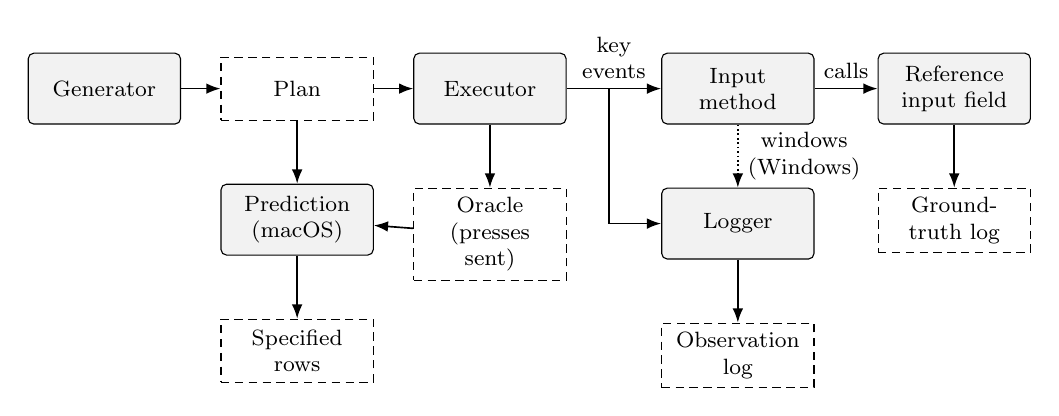
\begin{tikzpicture}[font=\footnotesize, node distance=8mm and 5mm,
  comp/.style={draw, rounded corners=2pt, align=center, minimum height=9mm, text width=17mm, fill=black!5},
  rec/.style={draw, densely dashed, align=center, minimum height=8mm, text width=17mm},
  arr/.style={-{Latex[length=1.8mm]}, semithick},
  lab/.style={font=\footnotesize, align=center}]
\node[comp] (gen) {Generator};
\node[rec, right=of gen] (plan) {Plan};
\node[comp, right=of plan] (exec) {Executor};
\node[comp, right=12mm of exec] (ime) {Input method};
\node[comp, right=8mm of ime] (ref) {Reference input field};
\node[rec, below=of exec] (oracle) {Oracle (presses sent)};
\node[comp, below=of plan] (pred) {Prediction (macOS)};
\node[rec, below=of pred] (spec) {Specified rows};
\node[comp, below=of ime] (logger) {Logger};
\node[rec, below=of logger] (obs) {Observation log};
\node[rec, below=of ref] (gt) {Ground-truth log};
\draw[arr] (gen) -- (plan);
\draw[arr] (plan) -- (exec);
\draw[arr] (exec) -- node[lab, above] {key\\events} coordinate[pos=0.45] (tap) (ime);
\draw[arr] (ime) -- node[lab, above] {calls} (ref);
\draw[arr] (exec) -- (oracle);
\draw[arr] (oracle) -- (pred);
\draw[arr] (plan) -- (pred);
\draw[arr] (pred) -- (spec);
\draw[arr] (tap) |- (logger.west);
\draw[arr, densely dotted] (ime) -- node[lab, right] {windows\\(Windows)} (logger);
\draw[arr] (logger) -- (obs);
\draw[arr] (ref) -- (gt);
\end{tikzpicture}
\caption{The components of a trial and the records they write (dashed boxes). The generator writes the plan from the
settings, the procedures, the phrase corpus and the seed. The executor sends the planned presses as system key events
and records each press as sent (the oracle). The reference input field records the calls that it receives from the
input method (the ground-truth log), and the logger writes its key and session rows (the observation log): on macOS
from the key presses and the input source, on Windows from the key presses and the windows of the input method. On
macOS the prediction computes, from the plan and the oracle alone, the rows that the logger's rules specify. The
ground-truth log and the observation log hold no text. The diagram is drawn by code written with an AI tool (Claude);
see the AI declaration}
\label{fig:components}
\end{figure}


\subsection{Cells, machines and settings}
\label{sec:method-cells}

The study had three cells. Two were on macOS: the standard Japanese input method of the system with live conversion
on, and the same input method with live conversion off. They were measured on one Apple Silicon computer with a JIS
keyboard and Romaji input, under macOS 27.0.1 (build 26A434; Romaji input method version 6.3), the same for every
macOS run. The third was on Windows: the Microsoft
input method (Japanese, Romaji input) with its default settings, measured on an x86-64 tablet computer (Intel Core
i5-1135G7, 8 GB of memory) with a JIS keyboard under Windows 11 Home 25H2 (build 26200.9457, input method
10.0.26100.9278). These versions differed from those of the Windows pilot (build 26200.8875, input method
10.0.26100.8875), so, as the addendum requires, the 39-trial check plan of the pilot was run first on the measuring
machine; every trial produced the session its plan intends (39 of 39), and the cell was measured. On both systems the
predictive candidates were left at their default (shown). The registration asks for each machine to run on mains power,
with automatic updates, network time synchronisation, sleep, the screen lock and the screen saver turned off; the run
manifests do not record these settings. What else ran on each machine is reported with the runs
(Section~\ref{sec:results-attempts}); on Windows the records show one automatic update during the completed run. On
Windows the runs were started from a terminal without administrator rights. The runs on both systems were started and
monitored by an AI coding assistant under the author's instructions (Declarations). The learning of the input method
was not reset at any point: no method of resetting it was found on macOS, and the Microsoft input method offers no
command that clears its input history. The run manifest of every run records the versions of the system, the input
method and the programs, and the outcome of every check of the front window.

On each machine the cells were measured in a fixed order (on macOS, live conversion on, then off), followed by the two
conditions of the runtime-cost study (Section~\ref{sec:cost}), so that the replay used for the runtime cost added no
learning to the input method before the agreement cells were measured. The registration asks for the runs to be made
on separate nights; on macOS each run was started as soon as the check of the one before it was done, so the runs
followed one another without overlapping (deviation D6). On Windows the cell was measured through the night and the
morning, the idle condition in the afternoon and evening of the same day and the working condition in the following
night, again in the registered order and without overlapping (deviation D9).

\subsection{Reference input fields and ground truth}
\label{sec:method-reference}

A reference input field is a minimal application that records what the input method tells it, and only that. Both
fields record times on the wall clock and on a monotonic clock, and neither records any text. The reference was placed
at this software layer because the question of the study is agreement with the calls that an application receives
from the input method, and no external device observes these calls. An external device, the usual standard for
validating timing instruments, could time the keys, the candidate window or the marked text on the screen; none of
these was done.\footnote{The registration gives the reason more broadly: that an external timing device would time
the path of the keys, not the conversion.} The comparison is therefore between two software records on the same
machine, not against an external standard: the physical path of the keys and the display are not exercised, no
external clock is used, and the reference is the sessions that one kind of field received, not the input method's
internal state (Section~\ref{sec:limitations}).

\paragraph{macOS.} The field implements the text-input client protocol of the macOS text system and records every call
that the input method makes to it: marked text set (with its length and the selected range), text inserted (with its
length), marked text accepted, a request for the position of the text, a command, each key-down it receives (key code
only) and each change of focus. It empties its text after every commit, so that no trial sees the text of an earlier
one. Sessions were assembled from its log by the following rules. A session opens at the first call that sets marked
text of positive length. It closes as committed at a call that inserts text of positive length, or that accepts the
marked text, when no call setting marked text of positive length follows within 50~ms. It closes as cancelled at a
call that sets marked text of length zero, when no call inserting text of positive length follows within 50~ms. With
live conversion the input method commits the head of a reading while the rest is still being typed; the 50~ms window
keeps such a commit inside its session. In the calibration pilot the following call came 0.5 to 7.9~ms after such a
commit, and every window between 10 and 900~ms gave the same sessions. The outcome of a session is the reason it
finally closed, and each session records how many of its commits were followed by a continuation.

\paragraph{Windows.} The field is a window with a rich-edit control that is a client of the Text Services Framework.
After each edit it reads the compositions of its document and records the start of a composition, its length after
each edit, its end with the length of the committed text (zero when nothing was committed, and no length when the
field closes a composition that it infers from a change of the composition's range or cannot read the committed
length), the beginning and end of the input method's user-interface elements with their kind, each change of focus,
and a key-down (key code only) for each key that the input method does not consume. A session runs from the start of
a composition to its end; it is committed when the committed length is positive and cancelled otherwise; it showed a
candidate window when the beginning of a user-interface element of the kind \emph{candidate} falls within it. Of the
two reference fields built for Windows, this one was chosen in the calibration pilot before any row of the logger was
read: the Microsoft input method is a text service of the framework, so its client receives the composition directly,
whereas a field that receives the input method's messages does so through a compatibility layer of the system; and
the latter field received the key press that switches the input method on before every block as a key-down, which
the rule on presses from outside (Section~\ref{sec:method-checks}) does not allow. The two fields also committed at
different points in one scenario of the pilot: in three trials of S7 the chosen field committed when the right arrow
was pressed past the last segment, whereas the other kept the composition until Return, so the kind of field affects
the reference.

\paragraph{Assignment and definitions.} A session is assigned to the trial that it overlaps most in wall-clock time.
Its true navigation count is the number of arrow presses that the oracle records as sent for that trial within the
session. A session is counted as lasting 20~s or more when its duration reaches 20{,}000~ms. Each system's logger
defines a session differently (Section~\ref{sec:logger}), so the ground truth was formed under the definition of the
cell's system: on macOS every session, and on Windows the sessions that showed a candidate window. The Microsoft input
method opens its prediction window, which the field reports as a candidate element, while the reading is typed, so on
Windows this definition holds nearly all sessions and does not mean that the reading was converted. The analysis was
also run under the definition common to both systems (every session); whether the two definitions hold the same
sessions is reported per cell, and where they do not, how many sessions the definition of the analysis leaves out and
the detection under the common definition, per stratum as ranges and pooled, are also reported (deviation D12, made
after the results had been seen).

\subsection{Scenarios, speeds and plans}
\label{sec:method-plans}

\paragraph{Scenarios.} Fifteen scenarios were designed to cover the ways a conversion can begin and end
(Table~\ref{tab:scenarios}). Scenario S9 (choosing a candidate with the mouse) had no procedure, because no means of
locating the candidate window for a scripted click was established; it was not run and is reported as not evaluated.
Scenario S11 (conversion without Space under live conversion) was run only with live conversion on. A cell therefore
had 14 scenarios (macOS, live conversion on) or 13 (macOS, live conversion off; Windows). With live conversion on, S3
and S11 share a procedure; they were kept apart because they were designed to test different behaviours of the input
method, and each is reported with its own trials. The procedures of each cell were fixed in its calibration pilot: with
live conversion off a single Return commits and a single Escape cancels a reading that was not converted, and on
Windows a single Return commits, a reading converted into several segments is cancelled only by a third Escape (S4),
a digit chooses a candidate without committing it (so S8 ends with a Return), and the input mode is switched with the
virtual keys that turn the input method on and off (S14).

\begin{table}[t]
\caption{Scenarios and their procedures (macOS, live conversion on). The last column gives the differences in the other
two cells}
\label{tab:scenarios}
\begin{tabular}{L{0.08}L{0.52}L{0.40}}
\toprule
& Procedure & Live conversion off; Windows \\
\midrule
S1 & Type the reading, Space, pause, Return twice (commit) & One Return \\
S2 & Type the reading, Space two to five times (cycling the candidates), pause, Return twice & Windows: one Return \\
S3 & Type the reading, Return (commit without conversion) & \\
S4 & Type the reading, Space, pause, Escape twice (cancel with the candidate window shown) & Windows: three Escapes \\
S5 & Type the reading, Escape four times (cancel without conversion) & One Escape \\
S6 & Type the reading, Backspace once per kana typed (delete everything) & \\
S7 & Type the reading, Space, right arrow one to three times, pause, Return twice & One Return \\
S8 & Type the reading, Space twice, pause, a digit choosing a candidate, Return & \\
S9 & Choose a candidate with the mouse & Not run in any cell \\
S10 & Type the first half of the reading, Tab (a predictive candidate), pause, Return & \\
S11 & Type the reading, Return (live conversion converts without Space) & Not run \\
S12 & Type a kana string with the kana keyboard layout, Space, Return twice & One Return \\
S13 & Type the reading, Space, wait 21~s, Return twice (a session over 20~s) & One Return \\
S14 & Type the reading, Space, switch the input mode off and on & Windows: with the virtual keys \\
S15 & Type the reading, Space, bring another application to the front for 1~s, return, Return twice & One Return \\
\bottomrule
\end{tabular}
\end{table}

\paragraph{Speeds and timing.} The interval between key presses was drawn from a log-normal distribution with a
median of 480~ms (slow), 240~ms (middle) or 120~ms (fast) and a log-scale standard deviation of 0.3. The medians
follow the per-participant mean inter-key intervals reported by \citet{dhakal2018} for the slowest tenth of their
participants, for all participants and for the fastest tenth; those values come from the transcription typing of
English sentences and were used to span the range of typing speeds, not as estimates of Japanese typing. Intervals
were drawn independently of the keys, and an interval shorter than the key hold plus 1~ms (61~ms) was raised to it,
which affected about 1\% of the intervals at the fast level. Each key was held for 60~ms, and no two presses
overlapped. In scenarios with a pause before the decisive key, the pause (think time) was drawn per trial from a
log-uniform distribution between 0.2 and 20~s, so that sessions fell on both sides of the logger's 20-second cut-off.
The candidate index was at most 4 (S2, S8), at most three arrow keys were pressed (S7), and the kana strings of S12,
typed with the kana keyboard layout, had four to eight characters.

\paragraph{Phrases.} The readings were taken from a corpus of 1{,}800 phrases, 150 from each of 12 public-domain works
in modern orthography obtained from Aozora Bunko \citep{aozora}. Each phrase is a run of clauses of a sentence whose
reading, assigned with the morphological analyser Sudachi \citep{takaoka2018} (SudachiPy 0.7.0 with the dictionary
sudachidict\_core 20260723.1, split mode~C), has 6 to 30 kana (median 16). Outside S12 the readings were typed in
Romaji; the reading assigned by the analyser, not the original text, is what was typed, so an incorrect reading
changes nothing in the evaluation.

\paragraph{Plans.} Each cell had one plan, generated from the settings, the cell's procedures, the corpus and the seed
20260929. A block held 25 trials of one speed. The order of the trials within each speed, the cut into blocks, the
order of the blocks and the order of the scenarios within a block were determined by the seed, and each trial drew its
phrase, key intervals, think time, candidate index and arrow count from a random state derived from the seed and the
trial's identifier. With 75 trials per scenario and speed, the plans held 3{,}150 trials in 126 blocks (live
conversion on), 2{,}925 trials in 117 blocks (live conversion off) and 2{,}925 trials in 117 blocks (Windows). The
plans were generated before each freeze on two versions of Python with byte-identical results, and their SHA-256 was
registered; a run whose plan had another SHA-256 was not analysed.

\paragraph{Precision plan.} The number of trials was chosen for the precision of the per-stratum proportions: near a
proportion of 0.95 the half-width of a 95\% Wilson interval is about 5 percentage points with 75 trials, which locates
such a proportion but does not guarantee that 0.95 and 0.90 are told apart. The number was not revised when the
prediction later showed how many trials the 20-second cut-off sets aside (Section~\ref{sec:method-analysis}); the
strata of the primary scope are therefore smaller. Outside S6 and S13 the smallest holds 31 trials on macOS and 32 on
Windows, which locate a proportion near 0.95 to within about 9 points; S13 is designed to exceed the cut-off and has
no trial in the primary scope, and S6, whose session Backspace keeps open, keeps as few as 3 trials at the slow speed
on macOS and 30 on Windows. Because the trials of a stratum fall into
several blocks that share the state of the input method, the design effect of the blocks within a stratum can reach
about 3.4, which widens an interval up to about 1.8 times; the Wilson intervals of pooled proportions ignore this and
are read as lower bounds of the uncertainty.

\paragraph{Running a cell.} The runner started the logger and then the reference input field. Before every block it
brought the field to the front, confirmed that the field was in front, and switched the input method on (with the
kana key on macOS and with the virtual key that turns the input method on in Windows). A block began with a marker of
four arrow presses (left, right, left, right) 150~ms apart, which both logs record and which is longer than any run of
arrow presses inside a trial; trials were separated by 1{,}000~ms. After the last block both programs ran for another
second before they were stopped. A run was aborted if a check of the front window failed or if either program stopped.

\paragraph{Executor.} The executor sent the planned presses as system key events (on Windows through the
\texttt{SendInput} interface) and recorded each press as sent, with its wall-clock and monotonic times taken
immediately before dispatch. It refused to start if either clock resolved more coarsely than 1~ms.

\subsection{Calibration pilots and blinding}
\label{sec:method-pilots}

A calibration pilot was run on each measuring machine before the freeze that covered it, with provisional settings
(fewer trials per scenario and speed, other seeds and, on macOS, other key-interval medians). On macOS six runs with
468 trials, about 87 minutes in all, were made; on Windows seven runs with 429 trials in 27 blocks, three with each of
the two reference fields and one check of the tools. The pilots fixed the procedures of each cell, the ground-truth
rules (including the 50~ms window), the settings of the stopping rule (Section~\ref{sec:method-checks}) and, on Windows,
the choice of the reference field. In the second macOS pilot the assembled sessions agreed with the plan's intent in
124 of 126 trials with live conversion on and 117 of 117 with it off, and in 39 of 39 trials of a check of the
procedures for live conversion off; on Windows, with the corrected procedures, every trial of the two check runs with
the chosen field produced the session its plan intends (39 of 39 each).

The logger's session rows were never read in the pilots. Before any analysis of a pilot run, each observation log was
split into its key rows, which were analysed, and its session rows, which were written to a sealed file padded to a
multiple of 1~MiB so that not even their number could be inferred. The key rows that were read are, on macOS, the very
input from which the logger infers its sessions; the blinding withheld the logger's output, not its input. The
ground-truth rules, the procedures, the analysis code and its settings were fixed without reference to any session row
of the logger, and no session row of the measurement was read before the freeze. The sealed rows are opened only to be
deposited with the pilots' raw logs (Section~\ref{sec:dataset}) and are not analysed.

\subsection{The rows the logger is specified to write}
\label{sec:method-prediction}

On macOS the logger's rules are deterministic functions of the key presses, so the rows it is specified to write can
be computed from the oracle and the plan. A program applied the rules, as written in the logger's source (the mapping
of key codes, the order in which a key updates the input-mode state and then drives the session, the transitions of a
session and the 20-second cut-off), to every press in the order and at the times that the oracle records, and also
modelled the runner's kana press and the marker presses. Its self-test compares its rule tables with the logger's
source. The result marks each trial as \emph{long} (a press of the trial entered a session that is cut off at 20~s),
\emph{carried out} (a session that the trial started does not end in it), \emph{received carry} (a press of the trial
entered a session started earlier) or \emph{closing key in reading} (the reading contains a key that closes a session
under the logger's rules, such as the minus, comma or period key).

The prediction separates two sources of disagreement. Three comparisons were computed with the same matching and the
same measures: ground truth against observation (the primary comparison), ground truth against prediction (how well
the rules, carried out exactly, describe the sessions of the reference field) and prediction against observation
(whether the logger carries out its rules). The tables call them reference vs.\ logger, reference vs.\ specified rows
and specified rows vs.\ logger, the specified rows being the rows of the prediction. The Windows logger follows the
input method's windows, which the presses do not determine, so no prediction applies to it, and only the primary
comparison was computed for the Windows cell.

\subsection{Checks of the instruments and the stopping rule}
\label{sec:method-checks}

\paragraph{Plan against ground truth.} For every trial the assembled sessions were compared with the plan's intent and
classified as agreeing or as one of six types of disagreement (no session, an unexpected session, several sessions, a
commit where a cancellation was planned, a cancellation where a commit was planned, a session open at the end). These
trials were kept in the evaluation: removing them would keep only the trials in which the input method behaved as
planned. Like the other checks of this section, this one is reported before the estimates of agreement and is used to
read them (for example, the observation rows of trials in which the reference lost the focus are reported separately,
so that a failure of the reference is not read as one of the logger); no check is used to exclude trials or to adjust
values.

\paragraph{Delivery.} A delivery report compared, press by press, the oracle with the plan, with the key rows of
presses in the observation and with the key-downs of the reference log: the delay of each press against the schedule,
the fraction of sent presses that reached each log, the rows without a sent press, and the timing of the rows. For
the timing, a trial was used when the rows of presses within its window (from 20~ms before its start to 300~ms after
its end) equalled its presses other than the input-mode keys; the $i$-th row was paired with the $i$-th press, the
delay of a row was its wall-clock time minus the executor's wall-clock time of dispatch, and the interval error was
the difference between consecutive rows minus that between the corresponding presses. Each was summarised per speed by
its number, mean, minimum, 5th percentile, median, 95th percentile and maximum, and the trials that could not be
paired were counted. The logger also writes a row for each key release, on both systems; no analysis uses these rows,
and the times of releases enter no measure.

\paragraph{Stopping rule.} Each cell was run once to completion, and a run that was aborted was repeated from the
start with the same plan, up to three attempts. A completed run also counted as aborted when its plan was not the
registered plan of its cell, when the delivery report refused its logs, when its reference log held key presses that
neither the executor nor the procedure explained (presses from outside), or when, within a loss of focus of the
reference field, the observation held a key row that no sent press explained. The rules on presses from outside and on
losses of focus were closed rules computed from the run's logs alone, with settings fixed from the pilots. On Windows
the reference field receives only the keys that the input method does not consume, so a run of the Windows cell also
counted as aborted when, in any segment of the run (the time before the first block, and each block), the key rows of
the observation that no sent press explained exceeded the marker presses of the segment (deviation D4). These rules
exist so that no person's typing enters the data; they were applied right after each run, before any analysis, and
every attempt is reported with its figures (Section~\ref{sec:results-attempts}). On Windows one attempt was stopped
from outside the runner and was counted as aborted, and one start from a terminal with administrator rights, which the
addendum excludes, was refused by the runner before its first trial and was not counted; this is recorded as deviation
D7.

\paragraph{Marker times.} The times at which the executor, the observation and the reference field recorded the
same block-marker presses were compared in every run and are reported. Their differences combine the offsets of the
processes' clocks with the delays of the paths by which each record receives a press, and the two cannot be separated
without an external clock. They were not used to correct the matching: the duration
error is a difference of durations, and a pair needs an overlap that tolerates a shift of up to a third of the length
of two intervals of equal length.

\subsection{Analysis of agreement}
\label{sec:method-analysis}

\paragraph{Exclusions.} Before matching, three kinds of trial were excluded and counted by reason and stratum: trials
after a step of the wall clock of more than 1{,}000~ms (to the end of the block), trials with a ground-truth session
still open when the reference log ends, and trials overlapped by a ground-truth session that ran from one trial into
another (a carry-over, which cannot be assigned to one trial). Observation rows were excluded with the trial they
overlap most. Trials in which the input method did not do what the plan intended, rows with a duration of zero (which
the logger writes when the wall clock steps back) and trials that the cut-off sets aside (below) were not excluded.

\paragraph{Scopes.} From the prediction, a trial is long when its presses entered a session that the logger's rules cut
off at 20~s; on Windows, where no prediction applies, a trial is long when the presses sent in it span at least 20~s
(deviation D3). The primary scope (\emph{under the limit}) holds the trials that are not long. Results are also given
over all trials and, for the cut-off, over the long trials alone. The scope is decided from what was sent, so it does
not depend on the observation. An estimate in the primary scope is always given with the fraction of trials that the
scope sets aside, the fraction excluded because a conversion ran from one trial into the next, and the estimate over
all trials, in the text or in the supplement.

\paragraph{Matching.} Sessions and observation rows were matched one to one in descending order of their intersection
over union, among the pairs that reach 0.5. A row's interval is the span of its duration ending at the time the row
was collected, which can be up to about 100~ms after the session ended; no offset or clock correction was applied. Among the items left unmatched, one session with two or more rows
whose combined interval reaches the criterion is a split, and one row with two or more sessions is a merge; the rest
are misses and false positives. A row lying at least half within a matched session is also counted toward a split,
and a session lying at least half within a matched row toward a merge, without changing the primary pairing.

\paragraph{Measures.} Question~1 (detection) is answered by recall (pairs over sessions), precision (pairs over rows),
the split, merge, miss and false-positive rates, and F1. Question~2 (per-session agreement) is answered, over the
pairs, by the error of the duration (the row's duration minus the session's), summarised by its median absolute value
and by the Bland--Altman bias and 95\% limits of agreement \citep{blandaltman1986}; by the agreement of the
abandonment flag with the session's outcome, as a two-by-two table, raw agreement and Cohen's kappa \citep{cohen1960}
per speed; and by the exact agreement of the navigation count with the arrow presses sent. For the cut-off, the rows of
20~s or more and the rows of the long trials are counted. Question~3 (per-text agreement) groups the trials of each
block, in plan order, into texts of eight trials and computes four aggregates on both sides: the conversions per
trial, the mean conversion time, the abandonment rate and the fraction of time spent converting. Agreement is reported
per speed by the Bland--Altman bias and limits of the per-text difference and by the intraclass correlation of a
two-way mixed model with the two methods as the only raters of interest, for absolute agreement of a single
measurement: ICC(A,1) in the notation of \citet{mcgrawwong1996}, which has the same value as ICC(2,1) of
\citet{shroutfleiss1979}, computed by the analysis code of the kit (\texttt{kit/analysis/stats.py}). The bias is also
reported for three mixtures of the speeds, and three per-trial differences are reported per scenario and speed so that
a reader can weight the scenarios differently. The bias, the limits of agreement, kappa and the ICC are the effect sizes
of this study; it tests no hypothesis, so no statistical power is computed, and the numbers of trials were set by the
precision plan above.

\paragraph{Exploratory analysis.} Not registered: because the errors of the duration have long tails, the 2.5th and
97.5th percentiles of the error and the fractions of pairs within 100~ms and within 1~s are reported for the pairs of
the primary comparison, without intervals. A script runs the frozen analysis unchanged, takes its pairs and requires
them to reproduce its number of pairs, bias and median absolute error at every speed before it computes these figures.

\paragraph{Intervals and wording.} The primary estimates are given per cell, scenario and speed. Proportions carry
95\% Wilson intervals \citep{wilson1927}. Continuous measures, the limits of agreement, kappa and the ICC carry 95\%
percentile bootstrap intervals \citep{efron1979} from 2{,}000 resamples of whole blocks \citep{cameron2008}, because
the trials of a block share the state of the input method. Pooled proportions carry Wilson intervals that ignore this
clustering and are read as lower bounds of the uncertainty. A value that cannot be computed is reported as missing with
its reason, never as zero; this includes an ICC whose reference has the same value in every text, which is zero
whatever the logger writes, or undefined if the logger writes that same value in every text too (deviation D11, made
after the results had been seen). Synthetic input has no natural mix of scenarios, so a pooled value is labelled as
pooled and is not an estimate of accuracy in natural typing. No threshold of adequate agreement was set,
and the estimates are described without evaluative words. Apart from the deviations (Section~\ref{sec:deviations}),
the one analysis not described in the registration is the exploratory analysis above, and it is labelled as such; the
comparisons between the cells or between speeds that the discussion reads are labelled as exploratory there.

\paragraph{Reproducibility.} The analyses were run from exports of the freezing tags: the registered analysis of
questions 1 to 3 with the matching code of the first change of deviation D10, which leaves the results of the frozen
code unchanged, the corrected analysis with its second change, and the closed-set attack with the switch of deviation
D8; each of these replaces one file of the export. Before any statistic, the analysis checked the freeze marks, the
SHA-256 of every log against its run manifest, the content-free format of every log, and the plan of every run, and it
refused a run that the stopping rule catches. The result files record the SHA-256 of the configuration, the rules,
every manifest and every log. The supplement lists, for every result file, the code it was made with, and the records
of the runs give the commands and the SHA-256 of every output. The result values of this article are copied from the
result files, or computed from them (the ranges over the strata, the counts of strata and the reference's standard
deviation between texts), by a script that is released with the code (\texttt{manuscript/tools/results\_tables.py}),
and the figures of the records (the attempts, the checks of the runs, the deviations) are copied from the records of
the runs (Declarations, Code availability). Statements that name strata or compare values, such as which strata set the
ends of a range, are written by hand from the generated values and tables and were checked by hand against them.

\subsection{Registration and deviations}
\label{sec:deviations}

The registration fixed the analysis in two ways. The configuration, the seed and the ground-truth rules are bound to the
registered file by a SHA-256 written into it (the freeze mark), which the analysis recomputes and checks before it
reads any data; the analysis code, the plan settings, the procedures and the corpus are fixed by the tag of the
freezing commit. The protocol was frozen in two stages (Table~\ref{tab:freezes}), each registered on OSF Registries
before the first measurement it covers \citep{prereg-macos,prereg-windows}. Each registration gives the 40-digit
identifier of its freezing commit and the SHA-256 of the list of files exported from it, so that the frozen materials
can be checked against the public repository. The addendum changed neither the configuration, the seed nor the
ground-truth rules, so the freeze mark kept its value; it carries the date of the second freeze, because the
addendum replaces the marks of the registered file.

\begin{table}[t]
\caption{The two freezes of the registration}
\label{tab:freezes}
\begin{tabular}{L{0.20}L{0.40}L{0.40}}
\toprule
& macOS cells & Windows addendum \\
\midrule
Frozen and registered & 2 October 2026 & 3 October 2026 \\
Tag & \texttt{ime-observation-prereg-macos} & \texttt{ime-observation-prereg-windows} \\
Files exported & 98 & 108 \\
Registration & \url{https://osf.io/9nh7r} & \url{https://osf.io/4jwzn} \\
\bottomrule
\end{tabular}
\end{table}

Thirteen deviations were recorded (Table~\ref{tab:deviations}): five for the Windows cell before the Windows
measurement, one for the macOS runs after their measurement and before their analysis (D6), two for the Windows runs
after their measurement (D7, before the analysis of the cell, and D9), one for the closed-set attack of all three
cells before that attack was run on any of them (D8), one for the analysis of questions 1 to 3 (D10), made when the
frozen analysis stopped on the macOS cells and before any of their results of these questions was seen, and three made
after all results had been seen: two for reporting, of the per-text ICC (D11) and of the detection under the
definition common to both systems on Windows (D12), both prompted by a simulated review of this article before its
submission (Declarations), and one for question 4 (D13), which corrects the description of three feature sets to what
the code computed and adds an exploratory analysis, prompted when the code was read for another study. D12 grew in two steps: it was recorded that the ranges of its per-stratum intervals would be reported
whatever their values before the ranges were computed, although the detection under the common definition had already
been seen, and the counts of the strata whose estimates change were added after the ranges had been seen, when a review
of the discussion found such changes. The registered results of questions 1 to 3
of the Windows cell, on which the frozen code did not stop, had been computed and committed before D10, and the
corrected analysis of D10 was applied to them as well. The
registration allowed the addendum to change only the Windows parts of existing files; deviations D1 to D4 touched
other parts. On the macOS cells they change nothing that is reported: the macOS plans generated with the changed
generator differ only in the recorded SHA-256 of a procedure file, the result files of the changed analysis code on
synthetic macOS runs are byte-identical to those of the macOS tag, and the macOS analysis was run from the macOS tag,
with the first change of D10 for questions 1 to 3 and the switch that D8 adds for the closed-set attack. The first
change of D10 left the result files of synthetic runs byte-identical to those of the frozen code; the corrected
analysis of its second change is reported next to the registered one for every cell.

% A long table (main.tex): as a float it is taller than the page of the template.
{\tablebodyfont
\begin{longtable}{L{0.08}L{0.46}L{0.46}}
\caption{Deviations from the registration}
\label{tab:deviations}\\
\toprule
& Change & Reason \\
\midrule
\endfirsthead
\tablecontinued{3}
\toprule
& Change & Reason \\
\midrule
\endhead
D1 & On Windows, scenario S4 presses Escape three times instead of twice. &
In the pilot two Escapes did not cancel a reading converted into several segments; the uncommitted reading ran into
the next trial. \\
D2 & The analysis accepts the registered plan of the Windows cell when the reference log comes from the field of the
Text Services Framework. &
The frozen check of the plan accepted only the two macOS plans, so no Windows run could have been analysed. \\
D3 & For the Windows cell a trial is long when the presses sent in it span at least 20~s. &
The prediction that defines long trials on macOS models the macOS logger and does not apply on Windows. \\
D4 & A Windows run counts as aborted when the observation holds, in any block, key rows that no sent press explains
beyond the block's marker presses. &
The Windows reference field receives only the keys that the input method does not consume, so a person typing into it
would otherwise pass the stopping rule. \\
D5 & The cell file of the Windows measurement names the two programs with backslashes. &
The runner could not start the programs from the relative paths of the template, which use forward slashes. \\
D6 & The macOS runs were made in the registered order, each started as soon as the check of the one before it was
done, not on separate nights. &
The operator did not wait for the next night; the order, which keeps the replay of the runtime-cost study after the
two cells, was kept, and no two runs overlapped. \\
D7 & On Windows an attempt stopped from outside the runner is counted as aborted, and a start refused by the runner
before its first trial, made with administrator rights, is not counted. &
The registration names neither event; the refused start was forbidden by the addendum and sent no key. \\
D8 & The closed-set attack leaves out every trial of scenario S12, through a switch added to the attack; without the
switch its output is that of the frozen code. &
The registration does not count the S12 trials, but the frozen code kept the 74 S12 trials of each plan whose phrase
is in the corpus, and stopped because too few decoys remained. \\
D9 & The Windows runs were made in the registered order, each started as soon as the check of the one before it was
done, not on separate nights. &
As for D6; the order was kept, and no two runs overlapped. \\
D10 & A rate whose numerator exceeds its denominator is reported without a value instead of stopping the analysis;
a corrected analysis, reported next to the registered one, counts a recounted merge in the stratum in which its
session row is counted. &
The frozen code counted a recounted merge in the stratum of the missed session, so the numerator of a stratum's
merge rate could exceed its denominator, and the analysis of the macOS cells stopped before it wrote any result. \\
D11 & The per-text ICC of a stratum whose reference has the same value in every text is reported without a value, with
the reason and next to the registered value, and the reference's standard deviation between texts is reported next to
every ICC. &
Such an ICC is zero whatever the logger writes (or undefined if the logger writes that same value in every text too); the
registration reports a measure with zero variance as missing, never as zero, but the frozen code returns no value only
when every value of both sides is the same. \\
D12 & On Windows, where the two definitions of a session do not hold the same sessions, how many sessions the
definition of the analysis leaves out and the detection under the common definition, per stratum as ranges and pooled,
are reported, with the number of strata whose estimate changes within the ranges and the largest change (added after
the ranges had been seen). &
The registration reports under the common definition only whether the two definitions hold the same sessions, which
does not show how far the estimates depend on the choice of definition. \\
D13 & The feature sets \texttt{no\_runs}, \texttt{bin1s\_count} and \texttt{counts\_only} are described as computed:
each run of letter keys is one token that keeps the number of its presses, so \texttt{counts\_only} holds the same
information as \texttt{no\_time}. Two sets without times that drop the lengths of runs are added as an exploratory
analysis, with the registered attack and rule, and do not change the recommendation (fixed after all results had been
seen and a related measurement of another study on the Windows cell). &
The registration describes these sets as having no lengths of letter runs, which the code does not do, so the
registered rule was applied to no set without those lengths. \\
\bottomrule
\end{longtable}
}

% Section 6 of the manuscript: what the reference establishes, detection and per-session agreement (questions 1 and
% 2). Every result value is read with \rv{} from generated/values.tex or given in a generated table; both are written
% by tools/results_tables.py from the result files. The table of attempts copies the records of experiment/data.md and
% experiment/data.windows.md.

\section{Results: what the reference establishes, detection and per-session agreement}
\label{sec:results}

The tables give the three cells side by side; the Windows values are read within their cell
(Section~\ref{sec:observability-consequence}).

\subsection{Runs and attempts}
\label{sec:results-attempts}

Each cell was measured in one completed run (Table~\ref{tab:attempts}). On macOS the first attempt of each cell
completed. On Windows the first attempt was stopped from outside the runner about 21 minutes after it began: the AI
coding assistant that had started the runner in a background shell ended that shell while the machine was short of
memory. The attempt wrote no run manifest and counts as aborted; in its logs the reference had no key-down that a press
does not explain and no span of lost focus held such a row, while the observation held 14 key rows beyond the marker
presses in its last segment, which the stop cut off. A later start from a terminal with administrator rights, which the
addendum excludes, was refused by the runner before its first trial and sent no key; it is not counted among the
attempts (deviation D7). The second attempt completed. In every completed run, including the runs of the working
condition of question~5, the plan had its registered SHA-256, the delivery report read the logs, and the figures of the
stopping rule (the key-downs of the reference that no press explains beyond the marker presses, before and in the last
block, the spans of a loss of focus with an observation row that no press explains, and on Windows the observation rows
beyond the marker presses) were zero. In the run of the macOS cell with live conversion off, the reference field lost
the focus once outside the plan, for 2.7~s; by the operator's report this was a pointer click on another window, which
the logs cannot confirm. The logs show no key press during it other than those sent: the 11 presses that the executor
sent in it did not reach the reference field, and every observation row in it had a sent press, so the run does not
count as aborted, and the trial it overlaps is analysed.

\paragraph{What else ran on the machines.} The registration does not restrict other programs, and the records give what
was known. On macOS the measuring machine also hosted a runner of a continuous-integration service, which was left
running; workflow runs of another project overlapped each run, for 23\% of the time of the run with live conversion on
(13 workflow runs), 20\% with it off (9), 13\% of the idle condition of question~5 (7) and 2\% of the working condition
(1), as upper bounds for the load on this machine; the times of the largest delays of the key rows
(Section~\ref{sec:results-reference}) were not compared with those of the workflow runs. On Windows, during the
completed run of the cell, the event logs show
one automatic update, of the definitions of the antivirus program, at 04:52 local time, eleven power-state events of a
system service and no restart; the log of the task scheduler was not enabled, so what it started cannot be told, and the
sessions of the AI coding assistant that ran on the machine were not read. The same was not recorded for the runs of
question~5 on Windows. This is what the records show, not a claim that nothing else ran.

\begin{table}[t]
\caption{Every attempt of every run of a plan, with the start that the runner refused. Aborted: whether the attempt
counts as aborted under the stopping rule of the registration. The idle condition of question~5 sends no key and has no
plan; its attempts are reported in Section~\ref{sec:cost}}
\label{tab:attempts}
\begin{tabular}{L{0.17}L{0.13}L{0.32}L{0.12}L{0.26}}
\toprule
Cell & Attempt & Course & Aborted & Deposited, and why \\
\midrule
macOS, live conversion on & 1 & Completed & No & Yes \\
macOS, live conversion off & 1 & Completed; one loss of focus of the reference outside the plan (2.7~s), with no key
press in the logs other than those sent & No & Yes \\
macOS, question~5, working & 1 & Completed & No & Yes \\
Windows & 1 & Stopped from outside the runner after about 21~minutes; no run manifest & Yes (incomplete) & No: stopped
inside a trial, so it does not pass the checks of the deposit (Section~\ref{sec:dataset-excluded}) \\
Windows & Not counted & Refused by the runner before the first trial (administrator rights); no key sent & No
(deviation D7) & Yes: refused before any key was sent, it passes the checks of the deposit
(Section~\ref{sec:dataset-excluded}) \\
Windows & 2 & Completed & No & Yes \\
Windows, question~5, working & 1 & Completed & No & Yes \\
\bottomrule
\end{tabular}
\end{table}

\subsection{What the reference establishes}
\label{sec:results-reference}

Table~\ref{tab:reference} gives the checks of the instruments, each with the estimates it is used to read; no check
excluded a trial or changed a value.

\paragraph{Plan against ground truth.} Of the trials of the plan, the sessions of the reference disagreed with the
plan's intent in \rv{macos-standard-live-off.plan.disagree} with live conversion off and in
\rv{macos-standard-live-on.plan.disagree} with live conversion on, and on Windows in
\rv{windows-msime-tsf.plan.disagree}. With live conversion on, most disagreements were trials without a session
(\rv{macos-standard-live-on.plan.no_session}), most of them in S10 at the slow and the middle speed (supplementary
table of the plan against the ground truth per stratum). Such trials stay in the evaluation; a trial without a
reference session has no session to detect, and its observation rows, if any, count as false positives.

\paragraph{Delivery.} Every planned trial was measured in each cell. The lateness of the presses against the schedule
had a median, a 95th percentile and a maximum of \rv{macos-standard-live-off.delivery.lateness} with live conversion
off, \rv{macos-standard-live-on.delivery.lateness} with it on, and \rv{windows-msime-tsf.delivery.lateness} on Windows.
The logger wrote a key row for every press other than the input-mode keys, which it does not record by design
(\rv{macos-standard-live-off.delivery.obs.nomode.reach}, \rv{macos-standard-live-on.delivery.obs.nomode.reach} and
\rv{windows-msime-tsf.delivery.obs.nomode.reach}), no trial held more key rows than presses sent, and the rows outside
every trial equal in number the marker presses of the blocks, four per block. On macOS the reference received
every press but those of the loss of focus described above (\rv{macos-standard-live-off.delivery.ref.nomode.reach} and
\rv{macos-standard-live-on.delivery.ref.nomode.reach}). On Windows the reference field receives only the keys that the
input method does not consume (Section~\ref{sec:method-reference}), so it received
\rv{windows-msime-tsf.delivery.ref.nomode.reach}, and the timing of its key-downs could not be paired in any trial.

\paragraph{Timing of the key rows.} Table~\ref{tab:key-timing} gives the delay of the logger's key rows of presses after
the executor dispatched them, and the error of the intervals between consecutive rows, per system and speed. Every
trial was paired (not paired: \rv{macos-standard-live-off.kt.obs.notpaired},
\rv{macos-standard-live-on.kt.obs.notpaired} and \rv{windows-msime-tsf.kt.obs.notpaired}). Over all speeds the median
delay was \rv{macos-standard-live-off.kt.obs.delay.all.median} and \rv{macos-standard-live-on.kt.obs.delay.all.median}
on macOS and \rv{windows-msime-tsf.kt.obs.delay.all.median} on Windows, with 95th percentiles of
\rv{macos-standard-live-off.kt.obs.delay.all.p95}, \rv{macos-standard-live-on.kt.obs.delay.all.p95} and
\rv{windows-msime-tsf.kt.obs.delay.all.p95} and maxima of \rv{macos-standard-live-off.kt.obs.delay.all.max},
\rv{macos-standard-live-on.kt.obs.delay.all.max} and \rv{windows-msime-tsf.kt.obs.delay.all.max}. The error of the
intervals is signed (the row's interval minus the interval sent), so its median says little about its spread: the
median was \rv{macos-standard-live-off.kt.obs.interval.all.median},
\rv{macos-standard-live-on.kt.obs.interval.all.median} and \rv{windows-msime-tsf.kt.obs.interval.all.median}, the 5th
and 95th percentiles \rv{macos-standard-live-off.kt.obs.interval.all.p05} and
\rv{macos-standard-live-off.kt.obs.interval.all.p95} with live conversion off,
\rv{macos-standard-live-on.kt.obs.interval.all.p05} and \rv{macos-standard-live-on.kt.obs.interval.all.p95} with it
on, and \rv{windows-msime-tsf.kt.obs.interval.all.p05} and \rv{windows-msime-tsf.kt.obs.interval.all.p95} on Windows,
and the extremes are given in the table. The report counts the trials that could not be paired over all
speeds, not per speed. These figures cover the software path from the dispatch of a synthetic event to the row
(Section~\ref{sec:method-reference}). The same figures for the key-downs of the macOS reference field are given in the
supplement.

\paragraph{Losses of focus.} Apart from the planned switches of S15, the reference field lost the focus once, in the
macOS run with live conversion off (\rv{macos-standard-live-off.focus.trialswithfocusloss} trial). The trial had no
session row (\rv{macos-standard-live-off.focus.rows.primary} in the primary scope), so this loss of focus gave no false
positive of detection.

\paragraph{Marker times.} On Windows the block-start marker was found in
\rv{windows-msime-tsf.markers.blocks} on every side. The observation minus the executor had a median of
\rv{windows-msime-tsf.markers.obsoracle.median} (range \rv{windows-msime-tsf.markers.obsoracle.range}), the reference
minus the executor \rv{windows-msime-tsf.markers.gtoracle.median} (range \rv{windows-msime-tsf.markers.gtoracle.range}),
and the observation minus the reference \rv{windows-msime-tsf.markers.obsgt.median} (range
\rv{windows-msime-tsf.markers.obsgt.range}); the fitted drifts were \rv{windows-msime-tsf.markers.obsoracle.drift},
\rv{windows-msime-tsf.markers.gtoracle.drift} and \rv{windows-msime-tsf.markers.obsgt.drift}. On macOS the
observation minus the reference had a median of \rv{macos-standard-live-off.markers.obsgt.median} with live conversion
off and \rv{macos-standard-live-on.markers.obsgt.median} with it on (ranges
\rv{macos-standard-live-off.markers.obsgt.range} and \rv{macos-standard-live-on.markers.obsgt.range}). Each difference
combines a clock offset with a path delay (Section~\ref{sec:method-checks}). The observation minus the executor is the
quantity that the delay of the key rows above measures, taken here at the marker presses only. The values per block
are given in the supplement.

\paragraph{What the reference does not establish.} The agreement of the logger with the reference is agreement between
two software records, not accuracy against an external standard, and the kind of field affects the reference
(Section~\ref{sec:method-reference}).

% Generated by manuscript/tools/results_tables.py from the result files; do not edit by hand.
\begin{sidewaystable}[p]
{\footnotesize
\caption{What the reference establishes, per cell: the agreement of the ground truth with the intent of the plan (count, and rate with its Wilson interval), the delivery of the presses that the executor sent (a / b: all presses / the input-mode keys left out, which the logger does not record by design), the losses of focus of the reference input field (a planned switch of S15 that returns within its trial is not counted as a trial with a loss) with the session rows assigned to the trials concerned, and the differences between the times at which the executor, the reference and the observation recorded the block-start markers, which combine the offsets of the clocks with the delays of the paths. Each group names the estimates it is used to read; no check excludes a trial or changes a value. Figures without an interval are descriptive; --: no value}
\label{tab:reference}
\begin{tabular}{L{0.34}L{0.220}L{0.220}L{0.220}}
\toprule
Figure & macOS, live conversion off & macOS, live conversion on & Windows \\
\midrule
\multicolumn{4}{L{1.000}}{\textit{Plan against ground truth, every trial of the plan}; read with misses in detection (Table~\ref{tab:detection}) and per-text agreement (Table~\ref{tab:text-agreement})} \\
Trials compared & 2{,}925 & 3{,}150 & 2{,}925 \\
Trials that disagree with the plan's intent & 0 (0.000 [0.000, 0.001]) & 100 (0.032 [0.026, 0.038]) & 1 (0.000 [0.000, 0.002]) \\
\quad No session & 0 (0.000 [0.000, 0.001]) & 94 (0.030 [0.024, 0.036]) & 0 (0.000 [0.000, 0.001]) \\
\quad An unexpected session & 0 (0.000 [0.000, 0.001]) & 0 (0.000 [0.000, 0.001]) & 0 (0.000 [0.000, 0.001]) \\
\quad Several sessions & 0 (0.000 [0.000, 0.001]) & 3 (0.001 [0.000, 0.003]) & 0 (0.000 [0.000, 0.001]) \\
\quad A commit where a cancellation was planned & 0 (0.000 [0.000, 0.001]) & 1 (0.000 [0.000, 0.002]) & 0 (0.000 [0.000, 0.001]) \\
\quad A cancellation where a commit was planned & 0 (0.000 [0.000, 0.001]) & 2 (0.001 [0.000, 0.002]) & 1 (0.000 [0.000, 0.002]) \\
\quad A session open at the end & 0 (0.000 [0.000, 0.001]) & 0 (0.000 [0.000, 0.001]) & 0 (0.000 [0.000, 0.001]) \\
\quad A trial not in the plan & 0 (0.000 [0.000, 0.001]) & 0 (0.000 [0.000, 0.001]) & 0 (0.000 [0.000, 0.001]) \\
Sessions assigned to no trial & 0 & 0 & 0 \\
\midrule
\multicolumn{4}{L{1.000}}{\textit{Delivery of the presses}; read with the timing of the key rows (Table~\ref{tab:key-timing}) and misses in detection} \\
Trials measured of those planned (incomplete) & 2{,}925 of 2{,}925 (0) & 3{,}150 of 3{,}150 (0) & 2{,}925 of 2{,}925 (0) \\
Presses sent & 93{,}861 / 93{,}411 & 103{,}182 / 102{,}732 & 93{,}861 / 93{,}411 \\
Lateness of the presses against the schedule (ms): median, 95th percentile, maximum & 2.30, 3.07, 315.34 & 2.25, 3.07, 456.13 & 0.05, 0.09, 140.83 \\
Observation: presses that arrived (rate) & 93{,}411 (0.995) / 93{,}411 (1.000) & 102{,}732 (0.996) / 102{,}732 (1.000) & 93{,}411 (0.995) / 93{,}411 (1.000) \\
Observation: trials with fewer rows than presses & 225 / 0 & 225 / 0 & 225 / 0 \\
Observation: rows beyond the presses sent in a trial (trials) & 0 (0) / 0 (0) & 0 (0) / 0 (0) & 0 (0) / 0 (0) \\
Observation: rows outside every trial & 468 / 468 & 504 / 504 & 468 / 468 \\
Reference: presses that arrived (rate) & 93{,}400 (0.995) / 93{,}400 (1.000) & 102{,}732 (0.996) / 102{,}732 (1.000) & 323 (0.003) / 323 (0.003) \\
Reference: trials with fewer rows than presses & 226 / 1 & 225 / 0 & 2{,}925 / 2{,}925 \\
Reference: rows beyond the presses sent in a trial (trials) & 0 (0) / 0 (0) & 0 (0) / 0 (0) & 0 (0) / 0 (0) \\
Reference: rows outside every trial & 468 / 468 & 504 / 504 & 468 / 468 \\
\midrule
\multicolumn{4}{L{1.000}}{\textit{Losses of focus of the reference input field}; read with false positives in detection} \\
Losses: planned switches of S15, others & 225, 1 & 225, 0 & 225, 0 \\
Other losses with key rows in the observation & 1 & 0 & 0 \\
Trials that overlap a loss & 1 & 0 & 0 \\
Session rows of these trials (false positives), primary scope & 0 (0) & 0 (0) & 0 (0) \\
Session rows of these trials (false positives), all trials & 0 (0) & 0 (0) & 0 (0) \\
\midrule
\multicolumn{4}{L{1.000}}{\textit{Times at which the block-start markers were recorded}; read with misses of short sessions in detection and the difference of \texttt{dwell\_ms} (Table~\ref{tab:session})} \\
Blocks with the marker found: executor, reference, observation & 117 of 117, 117, 117 & 126 of 126, 126, 126 & 117 of 117, 117, 117 \\
Observation minus executor (ms): median (range); drift per hour & 1 (0 to 97); $-$0.4 & 1.0 (0 to 97); $-$0.3 & 1 (0 to 2); 0.0 \\
Reference minus executor (ms): median (range); drift per hour & 3 (2 to 117); $-$0.5 & 3.0 (2 to 113); $-$0.3 & 5 (1 to 33); 0.1 \\
Reference minus executor, monotonic clocks (ms): median (range); drift per hour & 2.5 (2.0 to 116.8); $-$0.5 & 3.2 (2.4 to 113.8); $-$0.3 & 4.9 (1.5 to 33.2); 0.0 \\
Observation minus reference (ms): median (range); drift per hour & $-$2 ($-$20 to $-$1); 0.1 & $-$2.0 ($-$16 to $-$1); 0.0 & $-$4 ($-$31 to $-$1); $-$0.0 \\
\bottomrule
\end{tabular}
}
\end{sidewaystable}

% Generated by manuscript/tools/results_tables.py from the result files; do not edit by hand.
\begin{sidewaystable}[p]
{\footnotesize
\caption{Timing of the key rows of presses in the log on the software path, per cell and speed, in milliseconds, as the delivery report defines it: in the trials whose rows equal the presses sent other than the input-mode keys, the i-th row is paired with the i-th press; the delay is the time of the row minus the executor's time of dispatch, and the interval error is the difference between consecutive rows minus that between the consecutive presses. The times are whole milliseconds, so the minimum and the maximum are whole. The trials paired and not paired are given per cell, over all speeds, as the report gives them; --: no value}
\label{tab:key-timing}
\begin{tabular}{L{0.14}L{0.08}L{0.11}L{0.07}L{0.09}L{0.09}L{0.09}L{0.09}L{0.09}L{0.09}}
\toprule
Cell & Speed & Measure & n & Mean & Minimum & 5th percentile & Median & 95th percentile & Maximum \\
\midrule
macOS, live conversion off & slow & Delay & 30{,}945 & 1.6 & 0 & 1.0 & 2.0 & 2.0 & 55 \\
 &  & Interval error & 29{,}970 & 0.0 & $-$51 & $-$1.0 & 0.0 & 1.0 & 54 \\
 & mid & Delay & 31{,}423 & 1.4 & 0 & 0.0 & 1.0 & 2.0 & 95 \\
 &  & Interval error & 30{,}448 & $-$0.0 & $-$94 & $-$1.0 & 0.0 & 1.0 & 94 \\
 & fast & Delay & 31{,}043 & 1.4 & 0 & 0.0 & 1.0 & 2.0 & 26 \\
 &  & Interval error & 30{,}068 & $-$0.0 & $-$21 & $-$1.0 & 0.0 & 1.0 & 24 \\
 & all speeds & Delay & 93{,}411 & 1.5 & 0 & 0.0 & 1.0 & 2.0 & 95 \\
 &  & Interval error & 90{,}486 & $-$0.0 & $-$94 & $-$1.0 & 0.0 & 1.0 & 94 \\
 & \multicolumn{9}{l}{Trials paired: 2{,}925; not paired: 0} \\
macOS, live conversion on & slow & Delay & 34{,}063 & 1.4 & 0 & 0.0 & 1.0 & 2.0 & 20 \\
 &  & Interval error & 33{,}013 & $-$0.0 & $-$18 & $-$1.0 & 0.0 & 1.0 & 19 \\
 & mid & Delay & 34{,}743 & 1.3 & 0 & 0.0 & 1.0 & 2.0 & 24 \\
 &  & Interval error & 33{,}693 & $-$0.0 & $-$22 & $-$1.0 & 0.0 & 1.0 & 19 \\
 & fast & Delay & 33{,}926 & 1.2 & 0 & 0.0 & 1.0 & 2.0 & 30 \\
 &  & Interval error & 32{,}876 & $-$0.0 & $-$29 & $-$1.0 & 0.0 & 1.0 & 29 \\
 & all speeds & Delay & 102{,}732 & 1.3 & 0 & 0.0 & 1.0 & 2.0 & 30 \\
 &  & Interval error & 99{,}582 & $-$0.0 & $-$29 & $-$1.0 & 0.0 & 1.0 & 29 \\
 & \multicolumn{9}{l}{Trials paired: 3{,}150; not paired: 0} \\
Windows & slow & Delay & 30{,}945 & 1.2 & 0 & 0.0 & 1.0 & 2.0 & 5 \\
 &  & Interval error & 29{,}970 & 0.0 & $-$3 & $-$1.0 & 0.0 & 1.0 & 4 \\
 & mid & Delay & 31{,}423 & 1.2 & 0 & 0.0 & 1.0 & 2.0 & 3 \\
 &  & Interval error & 30{,}448 & $-$0.0 & $-$3 & $-$1.0 & 0.0 & 1.0 & 3 \\
 & fast & Delay & 31{,}043 & 1.1 & 0 & 0.0 & 1.0 & 2.0 & 3 \\
 &  & Interval error & 30{,}068 & $-$0.0 & $-$2 & $-$1.0 & 0.0 & 1.0 & 2 \\
 & all speeds & Delay & 93{,}411 & 1.1 & 0 & 0.0 & 1.0 & 2.0 & 5 \\
 &  & Interval error & 90{,}486 & $-$0.0 & $-$3 & $-$1.0 & 0.0 & 1.0 & 4 \\
 & \multicolumn{9}{l}{Trials paired: 2{,}925; not paired: 0} \\
\bottomrule
\end{tabular}
}
\end{sidewaystable}


\subsection{Detection}
\label{sec:results-detection}

\paragraph{Exclusions and scopes.} With live conversion off no trial was excluded; with it on, carry-over excluded
\rv{macos-standard-live-on.carryover}, and on Windows \rv{windows-msime-tsf.carryover}. No trial was excluded for a step
of the wall clock or a truncated log, and no session row had a duration of zero
(\rv{macos-standard-live-off.zerodwell.all}, \rv{macos-standard-live-on.zerodwell.all} and
\rv{windows-msime-tsf.zerodwell.all} over all trials). The primary scope set aside
\rv{macos-standard-live-off.scope.setaside} with live conversion off, \rv{macos-standard-live-on.scope.setaside} with
it on, and \rv{windows-msime-tsf.scope.setaside} on Windows. The supplement gives the number of letter keys and the
think time of the trials of each scope per stratum for the macOS cells, from the summary of the prediction; the analysis
of the Windows cell computes no prediction and gives no such summary.

\paragraph{Primary comparison and scope.} In the strata that keep at least 30 trials in the primary scope, the Wilson
intervals of recall spanned \rv{macos-standard-live-off.primary.recall.range} with live conversion off
(\rv{macos-standard-live-off.primary.recall.strata.left} strata left out),
\rv{macos-standard-live-on.primary.recall.range} with it on (\rv{macos-standard-live-on.primary.recall.strata.left} left
out) and, on Windows, \rv{windows-msime-tsf.primary.recall.range} (\rv{windows-msime-tsf.primary.recall.strata.left}
left out). Those of precision spanned \rv{macos-standard-live-off.primary.precision.range}
(\rv{macos-standard-live-off.primary.precision.strata.left} left out),
\rv{macos-standard-live-on.primary.precision.range} (\rv{macos-standard-live-on.primary.precision.strata.left} left out)
and \rv{windows-msime-tsf.primary.precision.range} (\rv{windows-msime-tsf.primary.precision.strata.left} left out). Over
all trials, both ranges were \rv{macos-standard-live-off.all.recall.range} and
\rv{macos-standard-live-off.all.precision.range} (\rv{macos-standard-live-off.all.recall.strata.left} and
\rv{macos-standard-live-off.all.precision.strata.left} strata left out), \rv{macos-standard-live-on.all.recall.range}
and \rv{macos-standard-live-on.all.precision.range} (\rv{macos-standard-live-on.all.recall.strata.left} and
\rv{macos-standard-live-on.all.precision.strata.left}), and \rv{windows-msime-tsf.all.recall.range} and
\rv{windows-msime-tsf.all.precision.range} (\rv{windows-msime-tsf.all.recall.strata.left} and
\rv{windows-msime-tsf.all.precision.strata.left}). Figure~\ref{fig:detection} shows every stratum with its interval,
Table~\ref{tab:detection} gives the ranges per speed, and the supplement gives every stratum with the split and merge
rates. Pooled over the strata of the primary scope (pooled values, whose Wilson intervals ignore the clustering of
trials in blocks and are read as lower bounds of the uncertainty; Section~\ref{sec:method-analysis}), recall was
\rv{macos-standard-live-off.pooled.gtobs.underlimit.recall}, \rv{macos-standard-live-on.pooled.gtobs.underlimit.recall}
and \rv{windows-msime-tsf.pooled.gtobs.underlimit.recall}, and precision
\rv{macos-standard-live-off.pooled.gtobs.underlimit.precision},
\rv{macos-standard-live-on.pooled.gtobs.underlimit.precision} and
\rv{windows-msime-tsf.pooled.gtobs.underlimit.precision}; over all trials, pooled recall was
\rv{macos-standard-live-off.pooled.gtobs.alltrials.recall}, \rv{macos-standard-live-on.pooled.gtobs.alltrials.recall}
and \rv{windows-msime-tsf.pooled.gtobs.alltrials.recall}.

\paragraph{What sets the ends of the ranges.} In both macOS cells the lowest intervals of the primary scope belong to
S6 and S10 at the fast speed, the two scenarios whose disagreement the registration expects from the logger's rules: in
S6 the logger keeps the session open while Backspace deletes the reading, and in S10 it closes the session at Tab,
which chooses a predictive candidate. On Windows the lowest recall belongs to S8 at the fast speed, which chooses a
candidate with a digit, with S2 and S1 at the fast speed close to it, and the lowest precision to S8 at the fast speed
and to S2, which cycles the candidates, at the middle and the fast speed. Over all trials the intervals of every cell
start at zero because of S13, whose sessions were built to outlast the 20-s cut-off: no row of the logger paired with
one of them (the macOS logger cuts such a session off without a row, and on Windows no row lasted 20~s or more), and
no stratum other than S13 has an interval that starts at zero. The strata left out of the ranges have fewer than 30
trials in the primary scope or no value there: the three strata of S13, which the scope sets aside entirely, in every
cell; S6 at the slow speed with live conversion off; and S6 at the slow and the middle speed and S10 at the slow speed
with it on. Over all trials the strata left out, which have fewer than 30 trials in that scope or no value there, were,
for recall, \rv{macos-standard-live-off.all.recall.strata.leftnames} with live conversion off,
\rv{macos-standard-live-on.all.recall.strata.leftnames} with it on and
\rv{windows-msime-tsf.all.recall.strata.leftnames} on Windows, and for precision
\rv{macos-standard-live-off.all.precision.strata.leftnames}, \rv{macos-standard-live-on.all.precision.strata.leftnames}
and \rv{windows-msime-tsf.all.precision.strata.leftnames}. A miss can come from
the timing of a row or from a difference between the lengths of the two constructs as well as from a session that the
logger did not detect, because a pair needs an intersection over union of 0.5 and no correction is applied
(Section~\ref{sec:method-analysis}).

\paragraph{Comparisons with the prediction (macOS).} The rules of the logger, carried out exactly on the presses sent,
described the reference sessions with recall intervals spanning \rv{macos-standard-live-off.gtpred.primary.recall.range}
with live conversion off and \rv{macos-standard-live-on.gtpred.primary.recall.range} with it on, and precision
intervals spanning \rv{macos-standard-live-off.gtpred.primary.precision.range} and
\rv{macos-standard-live-on.gtpred.primary.precision.range} (reference against the specified rows, primary scope). The
logger's rows agreed with the specified rows with recall intervals spanning
\rv{macos-standard-live-off.predobs.primary.recall.range} and \rv{macos-standard-live-on.predobs.primary.recall.range},
and precision intervals spanning \rv{macos-standard-live-off.predobs.primary.precision.range} and
\rv{macos-standard-live-on.predobs.primary.precision.range} (specified rows against the logger). Pooled over the primary
scope, the logger's rows agreed with the specified rows with recall
\rv{macos-standard-live-off.pooled.predobs.underlimit.recall} with live conversion off and
\rv{macos-standard-live-on.pooled.predobs.underlimit.recall} with it on, a miss rate of
\rv{macos-standard-live-off.pooled.predobs.underlimit.missrate} and
\rv{macos-standard-live-on.pooled.predobs.underlimit.missrate} and a false-positive rate of
\rv{macos-standard-live-off.pooled.predobs.underlimit.falseposrate} and
\rv{macos-standard-live-on.pooled.predobs.underlimit.falseposrate}, and the specified rows agreed with the reference
with recall \rv{macos-standard-live-off.pooled.gtpred.underlimit.recall} and
\rv{macos-standard-live-on.pooled.gtpred.underlimit.recall}. In the primary scope, the specified rows and the logger's
rows departed most in S12 at the middle and the fast speed in both cells; over the long trials, which the primary scope
sets aside, they departed most in S8, whose strata there hold few sessions (supplement). No arithmetic relation
between the three comparisons is claimed. The prediction marked, of the trials of the plan,
\rv{macos-standard-live-off.pred.trials.long}
and \rv{macos-standard-live-on.pred.trials.long} as long, \rv{macos-standard-live-off.pred.trials.carriedout} and
\rv{macos-standard-live-on.pred.trials.carriedout} as carrying a session out into the next trial,
\rv{macos-standard-live-off.pred.trials.receivedcarry} and \rv{macos-standard-live-on.pred.trials.receivedcarry} as
receiving one, and \rv{macos-standard-live-off.pred.trials.closingkeyinreading} and
\rv{macos-standard-live-on.pred.trials.closingkeyinreading} as holding a closing key inside a reading. In the trials
outside every layer, the primary scope gave recall \rv{macos-standard-live-off.layer.none.gtobs.primary.recall} and
precision \rv{macos-standard-live-off.layer.none.gtobs.primary.precision} for the reference against the logger with
live conversion off, and \rv{macos-standard-live-on.layer.none.gtobs.primary.recall} and
\rv{macos-standard-live-on.layer.none.gtobs.primary.precision} with it on; recall
\rv{macos-standard-live-off.layer.none.gtpred.primary.recall} and precision
\rv{macos-standard-live-off.layer.none.gtpred.primary.precision}, and
\rv{macos-standard-live-on.layer.none.gtpred.primary.recall} and
\rv{macos-standard-live-on.layer.none.gtpred.primary.precision}, for the reference against the specified rows; and
recall \rv{macos-standard-live-off.layer.none.predobs.primary.recall} and precision
\rv{macos-standard-live-off.layer.none.predobs.primary.precision}, and
\rv{macos-standard-live-on.layer.none.predobs.primary.recall} and
\rv{macos-standard-live-on.layer.none.predobs.primary.precision}, for the specified rows against the logger. The
supplement gives detection per layer of the prediction, for every comparison and scope.

\paragraph{The two definitions.} On macOS the definition of the analysis (every session) and the definition common to
both systems held the same sessions in both cells. On Windows they did not (the
definition of the analysis keeps the sessions in which the field reported a candidate element, which the input method
opens while the reading is typed); the estimates above are those of the definition of the analysis. Under deviation
D12, made after the results had been seen, the definition of the analysis left out
\rv{windows-msime-tsf.defs.primary.leftout} of the
\rv{windows-msime-tsf.defs.primary.common.sessions} reference sessions of the primary scope under the common definition
(\rv{windows-msime-tsf.defs.all.leftout} of \rv{windows-msime-tsf.defs.all.common.sessions} over all trials). Under
the common definition, the per-stratum Wilson intervals of recall spanned
\rv{windows-msime-tsf.defs.primary.common.recall.range} and those of precision
\rv{windows-msime-tsf.defs.primary.common.precision.range} in the primary scope
(\rv{windows-msime-tsf.defs.primary.common.recall.strata.left} and
\rv{windows-msime-tsf.defs.primary.common.precision.strata.left} strata left out), and
\rv{windows-msime-tsf.defs.all.common.recall.range} and \rv{windows-msime-tsf.defs.all.common.precision.range} over
all trials, against the ranges under the definition of the analysis given above. Within the ranges of the primary
scope, the estimates of single strata moved with the definition: the recall of
\rv{windows-msime-tsf.defs.primary.change.recall.strata} of the \rv{windows-msime-tsf.defs.primary.change.recall.of}
strata that enter both, by at most \rv{windows-msime-tsf.defs.primary.change.recall.max}, and the precision of
\rv{windows-msime-tsf.defs.primary.change.precision.strata} of \rv{windows-msime-tsf.defs.primary.change.precision.of}
(\rv{windows-msime-tsf.defs.primary.change.onlyone.note}), by at most
\rv{windows-msime-tsf.defs.primary.change.precision.max}; these counts were added after the ranges had been seen
(Section~\ref{sec:deviations}). Pooled over the primary scope under
the common definition, recall was \rv{windows-msime-tsf.defs.primary.common.recall}, precision
\rv{windows-msime-tsf.defs.primary.common.precision} and the merge rate
\rv{windows-msime-tsf.defs.primary.common.mergerate}, against \rv{windows-msime-tsf.pooled.gtobs.underlimit.recall},
\rv{windows-msime-tsf.pooled.gtobs.underlimit.precision} and \rv{windows-msime-tsf.pooled.gtobs.underlimit.mergerate}
under the definition of the analysis; the supplement gives both definitions in both scopes with the split rate.

\paragraph{Deviation D10.} The corrected analysis counts a recounted merge in the stratum of its paired row. It
changes the merge rate, and no other measure, in \rv{macos-standard-live-off.d10.primary.merge.differ} strata of the
primary scope with live conversion off, \rv{macos-standard-live-on.d10.primary.merge.differ} with it on and
\rv{windows-msime-tsf.d10.primary.merge.differ} on Windows. In the registered analysis
\rv{macos-standard-live-off.d10.layers.novalue} and \rv{macos-standard-live-on.d10.layers.novalue} merge rates of the
layers of the prediction have a numerator above their denominator and are reported without a value; the supplement
gives the registered and the corrected merge rate side by side, per stratum and per layer.

\paragraph{The cut-off.} No session row of 20~s or more was written in any cell
(\rv{macos-standard-live-off.cutoff.all.obsoverlimit}, \rv{macos-standard-live-on.cutoff.all.obsoverlimit} and
\rv{windows-msime-tsf.cutoff.all.obsoverlimit} over all trials). Of the reference sessions of 20~s or more that entered
the matching over all trials, \rv{macos-standard-live-off.cutoff.all.longwithrow} of
\rv{macos-standard-live-off.cutoff.all.long} with live conversion off and
\rv{macos-standard-live-on.cutoff.all.longwithrow} of \rv{macos-standard-live-on.cutoff.all.long} with it on appeared in
a pair, a split or a merge with a row of the logger, every row being shorter than 20~s; on Windows
\rv{windows-msime-tsf.cutoff.all.longwithrow} of \rv{windows-msime-tsf.cutoff.all.long} did. On the long trials alone,
pooled, the logger's rows agreed with the specified rows, which hold the sessions opened after a cut-off, with recall
\rv{macos-standard-live-off.pooled.predobs.overlimit.recall} and
\rv{macos-standard-live-on.pooled.predobs.overlimit.recall} and precision
\rv{macos-standard-live-off.pooled.predobs.overlimit.precision} and
\rv{macos-standard-live-on.pooled.predobs.overlimit.precision}. On Windows no row lasted from 20 to 25~s
(\rv{windows-msime-tsf.win.rows.20000to24999}) or 25~s or more (\rv{windows-msime-tsf.win.rows.25000ormore}), so the
rows give no indication of the window-event path or of its safety valve. That path has no cut-off at 20~s and can write
rows of 20~s or more, although a window shown again within a session starts it again without a row and the window need
not stay visible for the whole composition; the absence of such rows is consistent with the cloaking path, which writes
none, but does not show which path drove the input method. The plan made \rv{windows-msime-tsf.win.long.long}
of the \rv{windows-msime-tsf.win.long.trials} Windows trials long and the reference
\rv{windows-msime-tsf.win.long.longgt}; the two classified \rv{windows-msime-tsf.win.long.differ} trials differently,
and the reference session of \rv{windows-msime-tsf.win.long.band} trials lasted from 19 to 21~s. With the long trials
taken from the reference, pooled recall and precision in the primary scope were
\rv{windows-msime-tsf.pooled.gtobs.underlimitgtduration.recall} and
\rv{windows-msime-tsf.pooled.gtobs.underlimitgtduration.precision} (sensitivity analysis; per stratum in the
supplement).

\paragraph{Diagnostics.} On Windows the ends of a reference composition that carried no committed length were, per
scenario, \rv{windows-msime-tsf.win.endsnolength}; in S4 the reference session ended after the second of the three
Escapes in \rv{windows-msime-tsf.win.s4.escape2} trials and after the third in \rv{windows-msime-tsf.win.s4.escape3}. On
macOS the reference field receives the marked text again at every key, so a start event arrived while a session was open
in \rv{macos-standard-live-off.startwhileopen.all} of the \rv{macos-standard-live-off.pooled.gtobs.alltrials.sessions}
sessions with live conversion off and \rv{macos-standard-live-on.startwhileopen.all} of the
\rv{macos-standard-live-on.pooled.gtobs.alltrials.sessions} with it on (over all trials); on Windows in none
(\rv{windows-msime-tsf.startwhileopen.all}). Such an event opens no session.

% Generated by manuscript/tools/results_tables.py from the result files; do not edit by hand.
\begin{sidewaystable}[p]
\caption{Detection per cell, comparison and speed: the range from the lowest lower end to the highest upper end of the Wilson intervals of the scenarios that keep at least 30 trials and have a value of the measure, with the number of such scenarios and of all scenarios in parentheses, in the primary scope and over all trials. The comparisons with the prediction exist for the macOS cells only; --: no scenario in the range}
\label{tab:detection}
\begin{tabular}{L{0.17}L{0.12}L{0.07}L{0.16}L{0.16}L{0.16}L{0.16}}
\toprule
Cell & Comparison & Speed & Recall & Precision & Recall, all trials & Precision, all trials \\
\midrule
macOS, live conversion off & Reference vs. logger (primary) & slow & 0.715--1.000 (11/13) & 0.678--1.000 (11/13) & 0.000--0.963 (13/13) & 0.338--0.935 (12/13) \\
 &  & mid & 0.389--1.000 (12/13) & 0.413--1.000 (12/13) & 0.000--1.000 (13/13) & 0.000--1.000 (13/13) \\
 &  & fast & 0.280--0.992 (12/13) & 0.379--1.000 (12/13) & 0.000--0.986 (13/13) & 0.379--1.000 (12/13) \\
 & Reference vs. specified rows & slow & 0.715--1.000 (11/13) & 0.678--1.000 (11/13) & 0.000--0.963 (13/13) & 0.338--0.935 (12/13) \\
 &  & mid & 0.389--1.000 (12/13) & 0.413--1.000 (12/13) & 0.000--1.000 (13/13) & 0.000--1.000 (13/13) \\
 &  & fast & 0.280--0.992 (12/13) & 0.371--1.000 (12/13) & 0.000--0.986 (13/13) & 0.371--1.000 (12/13) \\
 & Specified rows vs. logger & slow & 0.893--1.000 (11/13) & 0.893--1.000 (11/13) & 0.646--1.000 (12/13) & 0.646--1.000 (12/13) \\
 &  & mid & 0.845--1.000 (12/13) & 0.845--1.000 (12/13) & 0.301--1.000 (13/13) & 0.301--1.000 (13/13) \\
 &  & fast & 0.848--1.000 (12/13) & 0.848--1.000 (12/13) & 0.795--1.000 (12/13) & 0.822--1.000 (12/13) \\
macOS, live conversion on & Reference vs. logger (primary) & slow & 0.830--1.000 (11/14) & 0.650--1.000 (11/14) & 0.000--0.962 (13/14) & 0.000--0.939 (13/14) \\
 &  & mid & 0.605--1.000 (12/14) & 0.559--1.000 (12/14) & 0.000--0.998 (14/14) & 0.000--0.998 (14/14) \\
 &  & fast & 0.301--1.000 (13/14) & 0.359--1.000 (13/14) & 0.000--1.000 (14/14) & 0.000--1.000 (14/14) \\
 & Reference vs. specified rows & slow & 0.830--1.000 (11/14) & 0.650--1.000 (11/14) & 0.000--0.962 (13/14) & 0.000--0.939 (13/14) \\
 &  & mid & 0.605--1.000 (12/14) & 0.559--1.000 (12/14) & 0.000--0.998 (14/14) & 0.000--0.998 (14/14) \\
 &  & fast & 0.331--1.000 (13/14) & 0.359--1.000 (13/14) & 0.000--1.000 (14/14) & 0.000--1.000 (14/14) \\
 & Specified rows vs. logger & slow & 0.886--1.000 (11/14) & 0.886--1.000 (11/14) & 0.207--1.000 (13/14) & 0.207--1.000 (13/14) \\
 &  & mid & 0.868--1.000 (12/14) & 0.868--1.000 (12/14) & 0.207--1.000 (14/14) & 0.207--1.000 (14/14) \\
 &  & fast & 0.815--1.000 (13/14) & 0.815--1.000 (13/14) & 0.207--1.000 (14/14) & 0.207--1.000 (14/14) \\
Windows & Reference vs. logger (primary) & slow & 0.799--1.000 (12/13) & 0.358--1.000 (12/13) & 0.000--1.000 (13/13) & 0.000--1.000 (13/13) \\
 &  & mid & 0.610--1.000 (12/13) & 0.328--1.000 (12/13) & 0.000--1.000 (13/13) & 0.000--1.000 (13/13) \\
 &  & fast & 0.412--1.000 (12/13) & 0.321--1.000 (12/13) & 0.000--1.000 (13/13) & 0.000--1.000 (13/13) \\
\bottomrule
\end{tabular}
\end{sidewaystable}

% Generated by manuscript/tools/results_tables.py from the result files; do not edit by hand.
\begin{sidewaysfigure}
\centering
\pgfplotslegendfromname{fig:detection:legend}\par\medskip
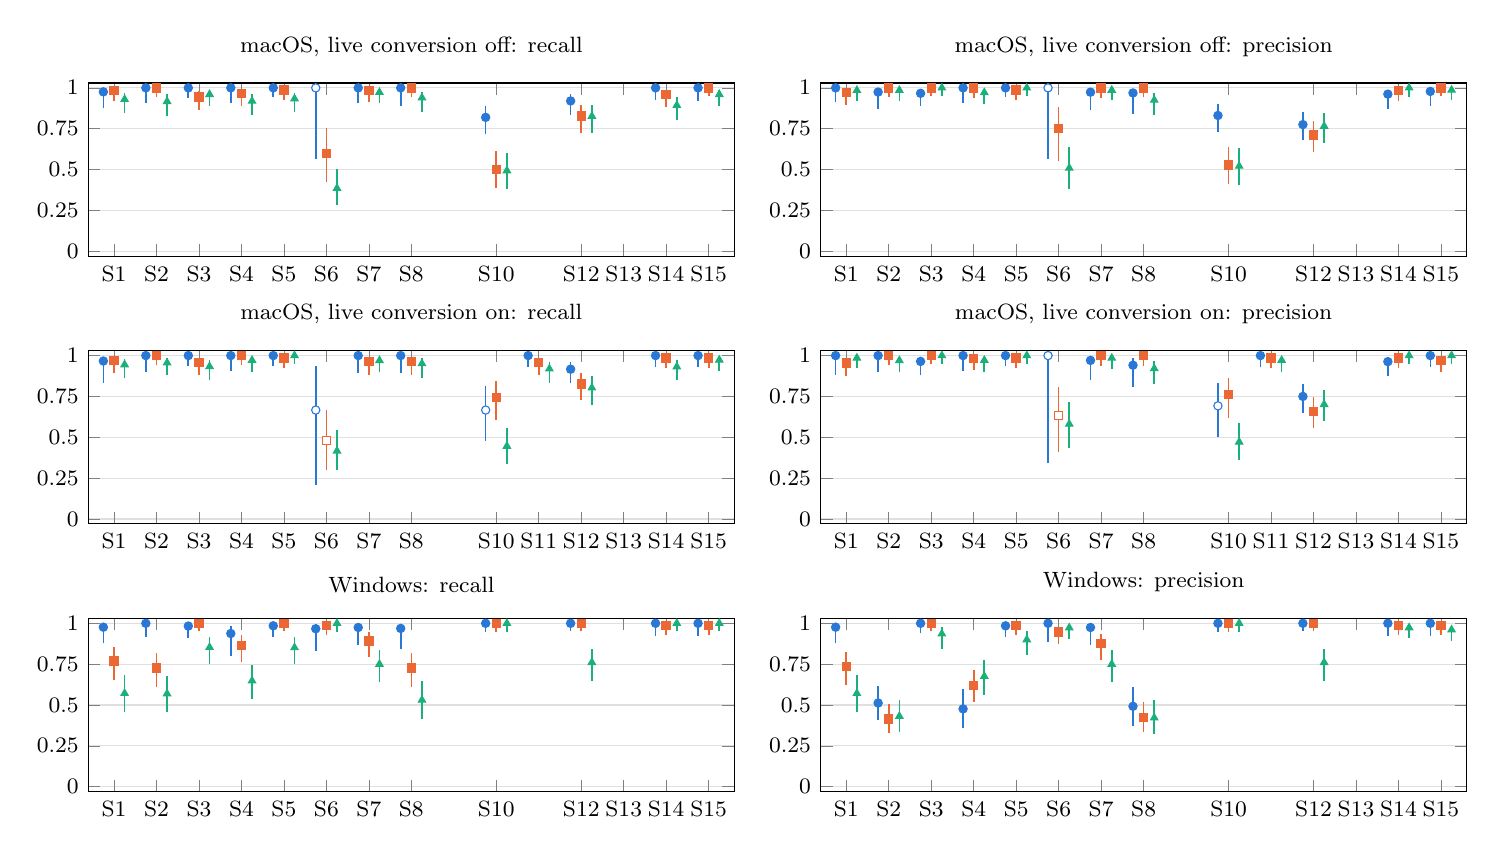
\begin{tikzpicture}
\begin{groupplot}[group style={group size=2 by 3, horizontal sep=1.1cm, vertical sep=1.2cm}, fig panel, fig proportion, scale only axis, width=8.2cm, height=2.2cm]
\nextgroupplot[xtick={1,2,3,4,5,6,7,8,10,12,13,14,15}, xticklabels={S1,S2,S3,S4,S5,S6,S7,S8,S10,S12,S13,S14,S15}, xmin=0.4, xmax=15.6, title={macOS, live conversion off: recall}, legend to name=fig:detection:legend, legend columns=4]
\addlegendimage{fig slow, fig point}
\addlegendentry{slow}
\addlegendimage{fig mid, fig point}
\addlegendentry{mid}
\addlegendimage{fig fast, fig point}
\addlegendentry{fast}
\addlegendimage{black, mark=*, fig point, fig open}
\addlegendentry{fewer than 30 trials}
\addplot[forget plot, fig interval, fig slow] table[row sep=\\] {x y\\0.75 0.874049\\0.75 0.995681\\0.75 nan\\1.75 0.90819\\1.75 1\\1.75 nan\\2.75 0.937882\\2.75 1\\2.75 nan\\3.75 0.905942\\3.75 1\\3.75 nan\\4.75 0.943376\\4.75 1\\4.75 nan\\5.75 0.565518\\5.75 1\\5.75 nan\\6.75 0.905942\\6.75 1\\6.75 nan\\7.75 0.889745\\7.75 1\\7.75 nan\\9.75 0.715197\\9.75 0.891332\\9.75 nan\\11.75 0.836252\\11.75 0.96282\\11.75 nan\\13.75 0.928652\\13.75 1\\13.75 nan\\14.75 0.921348\\14.75 1\\14.75 nan\\};
\addplot[forget plot, fig slow, fig point] table[row sep=\\] {x y\\0.75 0.97561\\1.75 1\\2.75 1\\3.75 1\\4.75 1\\6.75 1\\7.75 1\\9.75 0.819444\\11.75 0.92\\13.75 1\\14.75 1\\};
\addplot[forget plot, fig slow, fig point, fig open] table[row sep=\\] {x y\\5.75 1\\};
\addplot[forget plot, fig interval, fig mid] table[row sep=\\] {x y\\1 0.919041\\1 0.99732\\1 nan\\2 0.944198\\2 1\\2 nan\\3 0.86741\\3 0.978488\\3 nan\\4 0.886362\\4 0.990811\\4 nan\\5 0.924439\\5 0.997509\\5 nan\\6 0.423204\\6 0.754094\\6 nan\\7 0.911449\\7 0.997052\\7 nan\\8 0.943376\\8 1\\8 nan\\10 0.388926\\10 0.611074\\10 nan\\12 0.725692\\12 0.895809\\12 nan\\14 0.882976\\14 0.985527\\14 nan\\15 0.950008\\15 1\\15 nan\\};
\addplot[forget plot, fig mid, fig point] table[row sep=\\] {x y\\1 0.984848\\2 1\\3 0.945205\\4 0.966667\\5 0.985915\\6 0.6\\7 0.983333\\8 1\\10 0.5\\12 0.826667\\14 0.957746\\15 1\\};
\addplot[forget plot, fig interval, fig fast] table[row sep=\\] {x y\\1.25 0.84551\\1.25 0.969546\\1.25 nan\\2.25 0.829876\\2.25 0.961248\\2.25 nan\\3.25 0.88887\\3.25 0.986304\\3.25 nan\\4.25 0.834181\\4.25 0.96231\\4.25 nan\\5.25 0.853249\\5.25 0.97119\\5.25 nan\\6.25 0.280477\\6.25 0.502843\\6.25 nan\\7.25 0.905499\\7.25 0.992454\\7.25 nan\\8.25 0.854271\\8.25 0.976181\\8.25 nan\\10.25 0.3833\\10.25 0.604016\\10.25 nan\\12.25 0.725692\\12.25 0.895809\\12.25 nan\\14.25 0.803386\\14.25 0.944951\\14.25 nan\\15.25 0.88887\\15.25 0.986304\\15.25 nan\\};
\addplot[forget plot, fig fast, fig point] table[row sep=\\] {x y\\1.25 0.929577\\2.25 0.916667\\3.25 0.96\\4.25 0.918919\\5.25 0.933333\\6.25 0.385714\\7.25 0.972603\\8.25 0.939394\\10.25 0.493333\\12.25 0.826667\\14.25 0.893333\\15.25 0.96\\};
\nextgroupplot[xtick={1,2,3,4,5,6,7,8,10,12,13,14,15}, xticklabels={S1,S2,S3,S4,S5,S6,S7,S8,S10,S12,S13,S14,S15}, xmin=0.4, xmax=15.6, title={macOS, live conversion off: precision}]
\addplot[forget plot, fig interval, fig slow] table[row sep=\\] {x y\\0.75 0.912378\\0.75 1\\0.75 nan\\1.75 0.86819\\1.75 0.995459\\1.75 nan\\2.75 0.886362\\2.75 0.990811\\2.75 nan\\3.75 0.905942\\3.75 1\\3.75 nan\\4.75 0.943376\\4.75 1\\4.75 nan\\5.75 0.565518\\5.75 1\\5.75 nan\\6.75 0.865051\\6.75 0.995339\\6.75 nan\\7.75 0.842557\\7.75 0.994462\\7.75 nan\\9.75 0.727409\\9.75 0.900585\\9.75 nan\\11.75 0.678226\\11.75 0.849555\\11.75 nan\\13.75 0.870188\\13.75 0.989388\\13.75 nan\\14.75 0.886647\\14.75 0.996152\\14.75 nan\\};
\addplot[forget plot, fig slow, fig point] table[row sep=\\] {x y\\0.75 1\\1.75 0.974359\\2.75 0.966667\\3.75 1\\4.75 1\\6.75 0.973684\\7.75 0.96875\\9.75 0.830986\\11.75 0.775281\\13.75 0.961538\\14.75 0.978261\\};
\addplot[forget plot, fig slow, fig point, fig open] table[row sep=\\] {x y\\5.75 1\\};
\addplot[forget plot, fig interval, fig mid] table[row sep=\\] {x y\\1 0.897534\\1 0.991775\\1 nan\\2 0.944198\\2 1\\2 nan\\3 0.947263\\3 1\\3 nan\\4 0.937882\\4 1\\4 nan\\5 0.924439\\5 0.997509\\5 nan\\6 0.551006\\6 0.880006\\6 nan\\7 0.938871\\7 1\\7 nan\\8 0.943376\\8 1\\8 nan\\10 0.413219\\10 0.640951\\10 nan\\12 0.61016\\12 0.797143\\12 nan\\14 0.922369\\14 0.997437\\14 nan\\15 0.950008\\15 1\\15 nan\\};
\addplot[forget plot, fig mid, fig point] table[row sep=\\] {x y\\1 0.970149\\2 1\\3 1\\4 1\\5 0.985915\\6 0.75\\7 1\\8 1\\10 0.528571\\12 0.712644\\14 0.985507\\15 1\\};
\addplot[forget plot, fig interval, fig fast] table[row sep=\\] {x y\\1.25 0.920181\\1.25 0.99736\\1.25 nan\\2.25 0.920181\\2.25 0.99736\\2.25 nan\\3.25 0.949349\\3.25 1\\3.25 nan\\4.25 0.901677\\4.25 0.992129\\4.25 nan\\5.25 0.947977\\5.25 1\\5.25 nan\\6.25 0.378835\\6.25 0.638758\\6.25 nan\\7.25 0.925434\\7.25 0.997544\\7.25 nan\\8.25 0.83691\\8.25 0.967704\\8.25 nan\\10.25 0.40686\\10.25 0.633225\\10.25 nan\\12.25 0.662453\\12.25 0.844375\\12.25 nan\\14.25 0.945774\\14.25 1\\14.25 nan\\15.25 0.926403\\15.25 0.997578\\15.25 nan\\};
\addplot[forget plot, fig fast, fig point] table[row sep=\\] {x y\\1.25 0.985075\\2.25 0.985075\\3.25 1\\4.25 0.971429\\5.25 1\\6.25 0.509434\\7.25 0.986111\\8.25 0.925373\\10.25 0.521127\\12.25 0.765432\\14.25 1\\15.25 0.986301\\};
\nextgroupplot[xtick={1,2,3,4,5,6,7,8,10,11,12,13,14,15}, xticklabels={S1,S2,S3,S4,S5,S6,S7,S8,S10,S11,S12,S13,S14,S15}, xmin=0.4, xmax=15.6, title={macOS, live conversion on: recall}]
\addplot[forget plot, fig interval, fig slow] table[row sep=\\] {x y\\0.75 0.833296\\0.75 0.994091\\0.75 nan\\1.75 0.901099\\1.75 1\\1.75 nan\\2.75 0.933586\\2.75 1\\2.75 nan\\3.75 0.903581\\3.75 1\\3.75 nan\\4.75 0.936861\\4.75 1\\4.75 nan\\5.75 0.20766\\5.75 0.938508\\5.75 nan\\6.75 0.89573\\6.75 1\\6.75 nan\\7.75 0.892821\\7.75 1\\7.75 nan\\9.75 0.478248\\9.75 0.813567\\9.75 nan\\10.75 0.931208\\10.75 1\\10.75 nan\\11.75 0.829876\\11.75 0.961248\\11.75 nan\\13.75 0.931208\\13.75 1\\13.75 nan\\14.75 0.927302\\14.75 1\\14.75 nan\\};
\addplot[forget plot, fig slow, fig point] table[row sep=\\] {x y\\0.75 0.966667\\1.75 1\\2.75 1\\3.75 1\\4.75 1\\6.75 1\\7.75 1\\10.75 1\\11.75 0.916667\\13.75 1\\14.75 1\\};
\addplot[forget plot, fig slow, fig point, fig open] table[row sep=\\] {x y\\5.75 0.666667\\9.75 0.666667\\};
\addplot[forget plot, fig interval, fig mid] table[row sep=\\] {x y\\1 0.894573\\1 0.991521\\1 nan\\2 0.939828\\2 1\\2 nan\\3 0.882976\\3 0.985527\\3 nan\\4 0.940756\\4 1\\4 nan\\5 0.923418\\5 0.997474\\5 nan\\6 0.300313\\6 0.665015\\6 nan\\7 0.882709\\7 0.990492\\7 nan\\8 0.882709\\8 0.990492\\8 nan\\10 0.604918\\10 0.847468\\10 nan\\11 0.882976\\11 0.985527\\11 nan\\12 0.725692\\12 0.895809\\12 nan\\14 0.923418\\14 0.997474\\14 nan\\15 0.92129\\15 0.997399\\15 nan\\};
\addplot[forget plot, fig mid, fig point] table[row sep=\\] {x y\\1 0.969231\\2 1\\3 0.957746\\4 1\\5 0.985714\\7 0.965517\\8 0.965517\\10 0.744681\\11 0.957746\\12 0.826667\\14 0.985714\\15 0.985294\\};
\addplot[forget plot, fig mid, fig point, fig open] table[row sep=\\] {x y\\6 0.48\\};
\addplot[forget plot, fig interval, fig fast] table[row sep=\\] {x y\\1.25 0.86568\\1.25 0.978186\\1.25 nan\\2.25 0.878128\\2.25 0.984883\\2.25 nan\\3.25 0.853249\\3.25 0.97119\\3.25 nan\\4.25 0.901677\\4.25 0.992129\\4.25 nan\\5.25 0.951276\\5.25 1\\5.25 nan\\6.25 0.300643\\6.25 0.542719\\6.25 nan\\7.25 0.897534\\7.25 0.991775\\7.25 nan\\8.25 0.865089\\8.25 0.983134\\8.25 nan\\10.25 0.338158\\10.25 0.559069\\10.25 nan\\11.25 0.834181\\11.25 0.96231\\11.25 nan\\12.25 0.699562\\12.25 0.87658\\12.25 nan\\14.25 0.849479\\14.25 0.970391\\14.25 nan\\15.25 0.907885\\15.25 0.992656\\15.25 nan\\};
\addplot[forget plot, fig fast, fig point] table[row sep=\\] {x y\\1.25 0.944444\\2.25 0.955882\\3.25 0.933333\\4.25 0.971429\\5.25 1\\6.25 0.416667\\7.25 0.970149\\8.25 0.95082\\10.25 0.445946\\11.25 0.918919\\12.25 0.802632\\14.25 0.931507\\15.25 0.973333\\};
\nextgroupplot[xtick={1,2,3,4,5,6,7,8,10,11,12,13,14,15}, xticklabels={S1,S2,S3,S4,S5,S6,S7,S8,S10,S11,S12,S13,S14,S15}, xmin=0.4, xmax=15.6, title={macOS, live conversion on: precision}]
\addplot[forget plot, fig interval, fig slow] table[row sep=\\] {x y\\0.75 0.88303\\0.75 1\\0.75 nan\\1.75 0.901099\\1.75 1\\1.75 nan\\2.75 0.878812\\2.75 0.990151\\2.75 nan\\3.75 0.903581\\3.75 1\\3.75 nan\\4.75 0.936861\\4.75 1\\4.75 nan\\5.75 0.34238\\5.75 1\\5.75 nan\\6.75 0.850844\\6.75 0.994789\\6.75 nan\\7.75 0.809064\\7.75 0.983717\\7.75 nan\\9.75 0.500117\\9.75 0.834987\\9.75 nan\\10.75 0.931208\\10.75 1\\10.75 nan\\11.75 0.65037\\11.75 0.828717\\11.75 nan\\13.75 0.874648\\13.75 0.989784\\13.75 nan\\14.75 0.927302\\14.75 1\\14.75 nan\\};
\addplot[forget plot, fig slow, fig point] table[row sep=\\] {x y\\0.75 1\\1.75 1\\2.75 0.964286\\3.75 1\\4.75 1\\6.75 0.970588\\7.75 0.941176\\10.75 1\\11.75 0.75\\13.75 0.962963\\14.75 1\\};
\addplot[forget plot, fig slow, fig point, fig open] table[row sep=\\] {x y\\5.75 1\\9.75 0.692308\\};
\addplot[forget plot, fig interval, fig mid] table[row sep=\\] {x y\\1 0.874667\\1 0.984422\\1 nan\\2 0.939828\\2 1\\2 nan\\3 0.946529\\3 1\\3 nan\\4 0.914133\\4 0.997147\\4 nan\\5 0.923418\\5 0.997474\\5 nan\\6 0.410395\\6 0.808505\\6 nan\\7 0.935806\\7 1\\7 nan\\8 0.935806\\8 1\\8 nan\\10 0.620649\\10 0.860878\\10 nan\\11 0.922369\\11 0.997437\\11 nan\\12 0.559208\\12 0.74741\\12 nan\\14 0.923418\\14 0.997474\\14 nan\\15 0.900334\\15 0.992015\\15 nan\\};
\addplot[forget plot, fig mid, fig point] table[row sep=\\] {x y\\1 0.954545\\2 1\\3 1\\4 0.983871\\5 0.985714\\7 1\\8 1\\10 0.76087\\11 0.985507\\12 0.659574\\14 0.985714\\15 0.971014\\};
\addplot[forget plot, fig mid, fig point, fig open] table[row sep=\\] {x y\\6 0.631579\\};
\addplot[forget plot, fig interval, fig fast] table[row sep=\\] {x y\\1.25 0.922369\\1.25 0.997437\\1.25 nan\\2.25 0.897534\\2.25 0.991775\\2.25 nan\\3.25 0.947977\\3.25 1\\3.25 nan\\4.25 0.901677\\4.25 0.992129\\4.25 nan\\5.25 0.951276\\5.25 1\\5.25 nan\\6.25 0.433286\\6.25 0.716154\\6.25 nan\\7.25 0.919041\\7.25 0.99732\\7.25 nan\\8.25 0.827297\\8.25 0.965624\\8.25 nan\\10.25 0.359049\\10.25 0.586781\\10.25 nan\\11.25 0.901677\\11.25 0.992129\\11.25 nan\\12.25 0.598128\\12.25 0.787159\\12.25 nan\\14.25 0.946529\\14.25 1\\14.25 nan\\15.25 0.950008\\15.25 1\\15.25 nan\\};
\addplot[forget plot, fig fast, fig point] table[row sep=\\] {x y\\1.25 0.985507\\2.25 0.970149\\3.25 1\\4.25 0.971429\\5.25 1\\6.25 0.581395\\7.25 0.984848\\8.25 0.920635\\10.25 0.471429\\11.25 0.971429\\12.25 0.701149\\14.25 1\\15.25 1\\};
\nextgroupplot[xtick={1,2,3,4,5,6,7,8,10,12,13,14,15}, xticklabels={S1,S2,S3,S4,S5,S6,S7,S8,S10,S12,S13,S14,S15}, xmin=0.4, xmax=15.6, title={Windows: recall}]
\addplot[forget plot, fig interval, fig slow] table[row sep=\\] {x y\\0.75 0.876788\\0.75 0.995785\\0.75 nan\\1.75 0.916201\\1.75 1\\1.75 nan\\2.75 0.910043\\2.75 0.997002\\2.75 nan\\3.75 0.798529\\3.75 0.982689\\3.75 nan\\4.75 0.917867\\4.75 0.997279\\4.75 nan\\5.75 0.833296\\5.75 0.994091\\5.75 nan\\6.75 0.86819\\6.75 0.995459\\6.75 nan\\7.75 0.842557\\7.75 0.994462\\7.75 nan\\9.75 0.944997\\9.75 1\\9.75 nan\\11.75 0.951276\\11.75 1\\11.75 nan\\13.75 0.922926\\13.75 1\\13.75 nan\\14.75 0.922926\\14.75 1\\14.75 nan\\};
\addplot[forget plot, fig slow, fig point] table[row sep=\\] {x y\\0.75 0.97619\\1.75 1\\2.75 0.983051\\3.75 0.9375\\4.75 0.984615\\5.75 0.966667\\6.75 0.974359\\7.75 0.96875\\9.75 1\\11.75 1\\13.75 1\\14.75 1\\};
\addplot[forget plot, fig interval, fig mid] table[row sep=\\] {x y\\1 0.656032\\1 0.851921\\1 nan\\2 0.609578\\2 0.819967\\2 nan\\3 0.951276\\3 1\\3 nan\\4 0.760704\\4 0.926567\\4 nan\\5 0.951276\\5 1\\5 nan\\6 0.926403\\6 0.997578\\6 nan\\7 0.791014\\7 0.945999\\7 nan\\8 0.609578\\8 0.819967\\8 nan\\10 0.948672\\10 1\\10 nan\\12 0.951276\\12 1\\12 nan\\14 0.928266\\14 0.997642\\14 nan\\15 0.928266\\15 0.997642\\15 nan\\};
\addplot[forget plot, fig mid, fig point] table[row sep=\\] {x y\\1 0.768116\\2 0.727273\\3 1\\4 0.863636\\5 1\\6 0.986301\\7 0.890625\\8 0.727273\\10 1\\12 1\\14 0.986667\\15 0.986667\\};
\addplot[forget plot, fig interval, fig fast] table[row sep=\\] {x y\\1.25 0.454778\\1.25 0.680647\\1.25 nan\\2.25 0.454433\\2.25 0.677421\\2.25 nan\\3.25 0.750026\\3.25 0.918112\\3.25 nan\\4.25 0.535008\\4.25 0.747618\\4.25 nan\\5.25 0.753105\\5.25 0.914919\\5.25 nan\\6.25 0.948672\\6.25 1\\6.25 nan\\7.25 0.639065\\7.25 0.835609\\7.25 nan\\8.25 0.411577\\8.25 0.645696\\8.25 nan\\10.25 0.949349\\10.25 1\\10.25 nan\\12.25 0.649588\\12.25 0.844791\\12.25 nan\\14.25 0.950008\\14.25 1\\14.25 nan\\15.25 0.950008\\15.25 1\\15.25 nan\\};
\addplot[forget plot, fig fast, fig point] table[row sep=\\] {x y\\1.25 0.571429\\2.25 0.569444\\3.25 0.852941\\4.25 0.648649\\5.25 0.851351\\6.25 1\\7.25 0.75\\8.25 0.530303\\10.25 1\\12.25 0.760563\\14.25 1\\15.25 1\\};
\nextgroupplot[xtick={1,2,3,4,5,6,7,8,10,12,13,14,15}, xticklabels={S1,S2,S3,S4,S5,S6,S7,S8,S10,S12,S13,S14,S15}, xmin=0.4, xmax=15.6, title={Windows: precision}]
\addplot[forget plot, fig interval, fig slow] table[row sep=\\] {x y\\0.75 0.876788\\0.75 0.995785\\0.75 nan\\1.75 0.405908\\1.75 0.617391\\1.75 nan\\2.75 0.937882\\2.75 1\\2.75 nan\\3.75 0.357821\\3.75 0.597296\\3.75 nan\\4.75 0.917867\\4.75 0.997279\\4.75 nan\\5.75 0.88303\\5.75 1\\5.75 nan\\6.75 0.86819\\6.75 0.995459\\6.75 nan\\7.75 0.372668\\7.75 0.612371\\7.75 nan\\9.75 0.944997\\9.75 1\\9.75 nan\\11.75 0.951276\\11.75 1\\11.75 nan\\13.75 0.922926\\13.75 1\\13.75 nan\\14.75 0.922926\\14.75 1\\14.75 nan\\};
\addplot[forget plot, fig slow, fig point] table[row sep=\\] {x y\\0.75 0.97619\\1.75 0.512195\\2.75 1\\3.75 0.47619\\4.75 0.984615\\5.75 1\\6.75 0.974359\\7.75 0.492063\\9.75 1\\11.75 1\\13.75 1\\14.75 1\\};
\addplot[forget plot, fig interval, fig mid] table[row sep=\\] {x y\\1 0.624241\\1 0.824062\\1 nan\\2 0.328335\\2 0.504778\\2 nan\\3 0.951276\\3 1\\3 nan\\4 0.517457\\4 0.712088\\4 nan\\5 0.929163\\5 0.997674\\5 nan\\6 0.872343\\6 0.979345\\6 nan\\7 0.775485\\7 0.936295\\7 nan\\8 0.337589\\8 0.516915\\8 nan\\10 0.948672\\10 1\\10 nan\\12 0.951276\\12 1\\12 nan\\14 0.928266\\14 0.997642\\14 nan\\15 0.928266\\15 0.997642\\15 nan\\};
\addplot[forget plot, fig mid, fig point] table[row sep=\\] {x y\\1 0.736111\\2 0.413793\\3 1\\4 0.619565\\5 0.986842\\6 0.947368\\7 0.876923\\8 0.424779\\10 1\\12 1\\14 0.986667\\15 0.986667\\};
\addplot[forget plot, fig interval, fig fast] table[row sep=\\] {x y\\1.25 0.454778\\1.25 0.680647\\1.25 nan\\2.25 0.336558\\2.25 0.531918\\2.25 nan\\3.25 0.845525\\3.25 0.974627\\3.25 nan\\4.25 0.560612\\4.25 0.773428\\4.25 nan\\5.25 0.807671\\5.25 0.950711\\5.25 nan\\6.25 0.905499\\6.25 0.992454\\6.25 nan\\7.25 0.639065\\7.25 0.835609\\7.25 nan\\8.25 0.32123\\8.25 0.529072\\8.25 nan\\10.25 0.949349\\10.25 1\\10.25 nan\\12.25 0.649588\\12.25 0.844791\\12.25 nan\\14.25 0.907885\\14.25 0.992656\\14.25 nan\\15.25 0.890252\\15.25 0.986485\\15.25 nan\\};
\addplot[forget plot, fig fast, fig point] table[row sep=\\] {x y\\1.25 0.571429\\2.25 0.431579\\3.25 0.935484\\4.25 0.676056\\5.25 0.9\\6.25 0.972603\\7.25 0.75\\8.25 0.421687\\10.25 1\\12.25 0.760563\\14.25 0.973333\\15.25 0.960526\\};
\end{groupplot}
\end{tikzpicture}
\caption{Recall and precision of the session rows against the reference per scenario and speed, with 95\% Wilson intervals, per cell, in the primary comparison (reference vs. logger) and the primary scope. Open marks: strata that keep fewer than 30 trials in the scope, which the ranges given in the text leave out. A stratum with no trial or no value in the scope is not drawn; Table~\ref{tab:detection} and the supplement give every stratum. The figure is drawn from the result files by code written and reviewed with an AI tool (Claude) and checked by its tests; see the AI declaration}
\label{fig:detection}
\end{sidewaysfigure}


\subsection{Per-session agreement}
\label{sec:results-session}

Over the matched sessions of the primary scope, the per-speed intervals of the bias of \texttt{dwell\_ms} against the
duration of the reference session spanned \rv{macos-standard-live-off.primary.dwellbias.range} with live conversion
off, \rv{macos-standard-live-on.primary.dwellbias.range} with it on, and \rv{windows-msime-tsf.primary.dwellbias.range}
on Windows; over all trials, \rv{macos-standard-live-off.all.dwellbias.range},
\rv{macos-standard-live-on.all.dwellbias.range} and \rv{windows-msime-tsf.all.dwellbias.range}. A negative bias means
that the logger's duration was shorter than the reference's. Table~\ref{tab:session} gives the bias, the limits of
agreement and the median absolute difference per speed, with the agreement of \texttt{abandon} and \texttt{nav};
Figure~\ref{fig:dwell} shows the bias and the limits of agreement per stratum, and the supplement gives every stratum
and the comparisons with the prediction. On macOS, over the speeds of the primary scope, the limits of agreement of the
durations of the logger's rows against the specified rows spanned
\rv{macos-standard-live-off.predobs.primary.dwell.loa.span} with live conversion off and
\rv{macos-standard-live-on.predobs.primary.dwell.loa.span} with it on, with median absolute differences of
\rv{macos-standard-live-off.predobs.primary.dwell.mae.span} and
\rv{macos-standard-live-on.predobs.primary.dwell.mae.span}, and those of the specified rows against the reference
spanned \rv{macos-standard-live-off.gtpred.primary.dwell.loa.span} and
\rv{macos-standard-live-on.gtpred.primary.dwell.loa.span}, with median absolute differences of
\rv{macos-standard-live-off.gtpred.primary.dwell.mae.span} and
\rv{macos-standard-live-on.gtpred.primary.dwell.mae.span}. The differences have long tails: in every cell and at every
speed the median absolute difference was less than a tenth of the distance between the limits of agreement
(Table~\ref{tab:session}), so the limits, which assume normally distributed differences, describe neither the typical
pair nor the largest differences. In the exploratory analysis of their distribution in the primary scope (not
registered; ranges over the speeds, every speed and scope in the supplement), the fraction of pairs within 100~ms was
\rv{macos-standard-live-off.dwellx.within100.range} with live conversion off,
\rv{macos-standard-live-on.dwellx.within100.range} with it on and \rv{windows-msime-tsf.dwellx.within100.range} on
Windows, and within 1~s \rv{macos-standard-live-off.dwellx.within1000.range},
\rv{macos-standard-live-on.dwellx.within1000.range} and \rv{windows-msime-tsf.dwellx.within1000.range}; the 2.5th
percentile was \rv{macos-standard-live-off.dwellx.p25.range}, \rv{macos-standard-live-on.dwellx.p25.range} and
\rv{windows-msime-tsf.dwellx.p25.range}, and the 97.5th \rv{macos-standard-live-off.dwellx.p975.range},
\rv{macos-standard-live-on.dwellx.p975.range} and \rv{windows-msime-tsf.dwellx.p975.range}.

The agreement of \texttt{abandon} with the outcome of the session was, pooled over the primary scope, for the sessions
whose commit was followed by a continuation, \rv{macos-standard-live-on.abandon.continued.with.primary} with live
conversion on, and for the other sessions \rv{macos-standard-live-off.abandon.continued.without.primary} with live
conversion off, \rv{macos-standard-live-on.abandon.continued.without.primary} with it on and
\rv{windows-msime-tsf.abandon.continued.without.primary} on Windows; with live conversion off and on Windows no session
had a continued commit. On Windows \texttt{nav} and \texttt{abandon} count presses system-wide while a session is open,
so by their rule they are upper bounds; in this design only the executor typed, and the per-text abandonment rate of the
Windows logger was lower than the reference's, with a bias of \rv{windows-msime-tsf.l2.abandon_rate.slow.bias},
\rv{windows-msime-tsf.l2.abandon_rate.mid.bias} and \rv{windows-msime-tsf.l2.abandon_rate.fast.bias} at the slow, the
middle and the fast speed (Table~\ref{tab:text-agreement}); where the difference comes from was not analysed.

% Generated by manuscript/tools/results_tables.py from the result files; do not edit by hand.
\begin{sidewaystable}[p]
{\footnotesize
\caption{Per-session agreement per cell and speed, primary comparison and scope: the difference of \texttt{dwell\_ms} from the duration of the reference session (bias, limits of agreement and median absolute difference, each with a 95\% interval that resamples blocks), the agreement of \texttt{abandon} with the outcome of the session (raw agreement with its Wilson interval and kappa with its block interval), and the exact agreement of \texttt{nav} with the arrow presses sent (Wilson interval); Pairs is the number of matched sessions with a duration on both sides. An estimate printed without an interval has its interval withheld (the reason is in the result file); --: no value}
\label{tab:session}
\begin{tabular}{L{0.12}L{0.06}L{0.06}L{0.11}L{0.11}L{0.11}L{0.11}L{0.11}L{0.11}L{0.10}}
\toprule
Cell & Speed & Pairs & Bias (ms) & Lower limit (ms) & Upper limit (ms) & Median absolute difference (ms) & \texttt{abandon} agreement & \texttt{abandon} kappa & \texttt{nav} exact \\
\midrule
macOS, live conversion off & slow & 533 & $-$427 [$-$561, $-$300] & $-$3,236 [$-$3,811, $-$2,650] & 2,382 [1,935, 2,801] & 36 [32, 41] & 0.991 [0.978, 0.996] & 0.970 [0.945, 0.993] & 0.996 [0.986, 0.999] \\
 & mid & 708 & $-$2 [$-$76, 80] & $-$2,213 [$-$2,560, $-$1,809] & 2,208 [1,707, 2,667] & 39 [36, 44] & 0.980 [0.967, 0.988] & 0.937 [0.902, 0.968] & 0.999 [0.992, 1.000] \\
 & fast & 740 & 124 [53, 201] & $-$2,034 [$-$2,342, $-$1,693] & 2,283 [1,821, 2,723] & 44 [40, 48] & 0.969 [0.954, 0.979] & 0.906 [0.866, 0.941] & 1.000 [0.995, 1.000] \\
macOS, live conversion on & slow & 515 & $-$544 [$-$656, $-$447] & $-$3,010 [$-$3,775, $-$2,220] & 1,922 [1,283, 2,508] & 384 [352, 407] & 0.996 [0.986, 0.999] & 0.987 [0.967, 1.000] & 1.000 [0.993, 1.000] \\
 & mid & 746 & $-$82 [$-$165, 14] & $-$2,378 [$-$2,766, $-$1,926] & 2,215 [1,646, 2,772] & 171 [149, 191] & 0.985 [0.974, 0.992] & 0.951 [0.923, 0.974] & 0.996 [0.988, 0.999] \\
 & fast & 797 & 86 [15, 156] & $-$2,059 [$-$2,319, $-$1,749] & 2,230 [1,810, 2,618] & 97 [86, 104] & 0.971 [0.957, 0.981] & 0.909 [0.869, 0.944] & 0.999 [0.993, 1.000] \\
Windows & slow & 566 & $-$934 [$-$1,055, $-$823] & $-$3,491 [$-$3,889, $-$3,090] & 1,623 [1,405, 1,832] & 480 [446, 531] & 0.896 [0.868, 0.918] & 0.629 [0.537, 0.717] & 1.000 [0.993, 1.000] \\
 & mid & 779 & $-$1,006 [$-$1,121, $-$892] & $-$4,321 [$-$4,738, $-$3,883] & 2,310 [2,068, 2,526] & 276 [248, 308] & 0.836 [0.808, 0.860] & 0.467 [0.409, 0.523] & 0.969 [0.955, 0.979] \\
 & fast & 682 & $-$550 [$-$654, $-$456] & $-$2,860 [$-$3,215, $-$2,507] & 1,760 [1,508, 2,013] & 178 [162, 197] & 0.824 [0.794, 0.851] & 0.431 [0.361, 0.504] & 0.921 [0.898, 0.939] \\
\bottomrule
\end{tabular}
}
\end{sidewaystable}

% Generated by manuscript/tools/results_tables.py from the result files; do not edit by hand.
\begin{figure}[p]
\centering
\pgfplotslegendfromname{fig:dwell:legend}\par\medskip
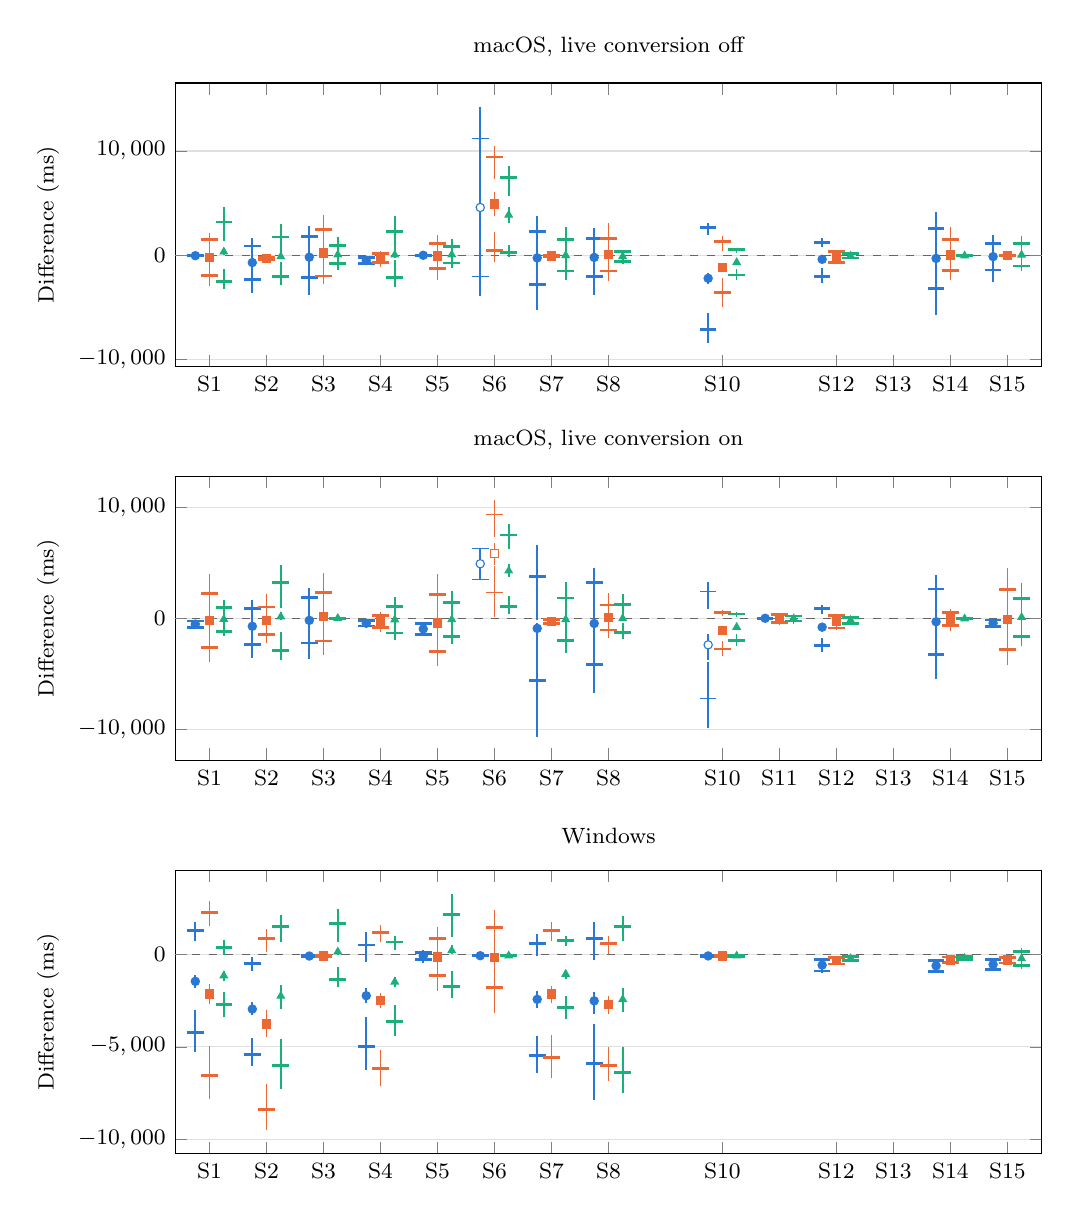
\begin{tikzpicture}
\begin{groupplot}[group style={group size=1 by 3, vertical sep=1.4cm}, fig panel, fig zero, scale only axis, width=11cm, height=3.6cm, ylabel={Difference (ms)}]
\nextgroupplot[xtick={1,2,3,4,5,6,7,8,10,12,13,14,15}, xticklabels={S1,S2,S3,S4,S5,S6,S7,S8,S10,S12,S13,S14,S15}, xmin=0.4, xmax=15.6, title={macOS, live conversion off}, legend to name=fig:dwell:legend, legend columns=5]
\addlegendimage{fig slow, fig point}
\addlegendentry{slow}
\addlegendimage{fig mid, fig point}
\addlegendentry{mid}
\addlegendimage{fig fast, fig point}
\addlegendentry{fast}
\addlegendimage{black, mark=*, fig point, fig open}
\addlegendentry{fewer than 30 trials}
\addlegendimage{black, fig limit}
\addlegendentry{limit of agreement}
\addplot[forget plot, fig interval, fig slow] table[row sep=\\] {x y\\0.75 -75.4257\\0.75 -59.8758\\0.75 nan\\1.75 -3576.2\\1.75 -788.026\\1.75 nan\\2.75 -3836.69\\2.75 -12.8138\\2.75 nan\\3.75 -964.032\\3.75 -673.412\\3.75 nan\\4.75 -2.77561\\4.75 -1.15887\\4.75 nan\\5.75 -3894.67\\5.75 2428.29\\5.75 nan\\6.75 -5294.56\\6.75 -58.5008\\6.75 nan\\7.75 -3803.61\\7.75 -62.4587\\7.75 nan\\9.75 -8392.22\\9.75 -5524.22\\9.75 nan\\11.75 -2688.81\\11.75 -1211.37\\11.75 nan\\13.75 -5732.33\\13.75 -60.6085\\13.75 nan\\14.75 -2605.38\\14.75 -51.3518\\14.75 nan\\};
\addplot[forget plot, fig slow, fig limit] table[row sep=\\] {x y\\0.75 -67.9431\\1.75 -2287.54\\2.75 -2154.02\\3.75 -819.049\\4.75 -2.02907\\6.75 -2806.82\\7.75 -1998.27\\9.75 -7109.15\\11.75 -2020.98\\13.75 -3158.57\\14.75 -1421.75\\};
\addplot[forget plot, fig slow, fig limit, fig open] table[row sep=\\] {x y\\5.75 -1993.26\\};
\addplot[forget plot, fig interval, fig mid] table[row sep=\\] {x y\\1 -2972.49\\1 -79.9924\\1 nan\\2 -439.694\\2 -378.312\\2 nan\\3 -2770.1\\3 -13.2494\\3 nan\\4 -1118.01\\4 -359.053\\4 nan\\5 -2405.32\\5 -0.811858\\5 nan\\6 -664.863\\6 2212.17\\6 nan\\7 -106.049\\7 -82.7035\\7 nan\\8 -2509.56\\8 -76.4093\\8 nan\\10 -4917.99\\10 -2130.87\\10 nan\\12 -838.405\\12 -526.477\\12 nan\\14 -2322.07\\14 -63.3582\\14 nan\\15 -78.9387\\15 -62.4595\\15 nan\\};
\addplot[forget plot, fig mid, fig limit] table[row sep=\\] {x y\\1 -1910.67\\2 -410.282\\3 -1978.41\\4 -722.404\\5 -1285.46\\6 434.382\\7 -95.1332\\8 -1516.85\\10 -3585.63\\12 -693.272\\14 -1480.26\\15 -71.0878\\};
\addplot[forget plot, fig interval, fig fast] table[row sep=\\] {x y\\1.25 -3240.45\\1.25 -1270.83\\1.25 nan\\2.25 -2882.41\\2.25 -611.772\\2.25 nan\\3.25 -1400.12\\3.25 -10.1817\\3.25 nan\\4.25 -3004.22\\4.25 -434.894\\4.25 nan\\5.25 -1257.83\\5.25 -1.61752\\5.25 nan\\6.25 -137.645\\6.25 989.54\\6.25 nan\\7.25 -2394.05\\7.25 -84.8501\\7.25 nan\\8.25 -789.422\\8.25 -264.137\\8.25 nan\\10.25 -2334.04\\10.25 -1343.92\\10.25 nan\\12.25 -354.956\\12.25 -158.428\\12.25 nan\\14.25 -86.7069\\14.25 -64.9602\\14.25 nan\\15.25 -1507.34\\15.25 -82.4561\\15.25 nan\\};
\addplot[forget plot, fig fast, fig limit] table[row sep=\\] {x y\\1.25 -2513.5\\2.25 -2015.25\\3.25 -810.647\\4.25 -2163.62\\5.25 -745.711\\6.25 280.151\\7.25 -1517.85\\8.25 -569.181\\10.25 -1880.23\\12.25 -261.718\\14.25 -76.4071\\15.25 -1038.1\\};
\addplot[forget plot, fig interval, fig slow] table[row sep=\\] {x y\\0.75 -13.412\\0.75 -0.642795\\0.75 nan\\1.75 -323.458\\1.75 1684.76\\1.75 nan\\2.75 3.33828\\2.75 2827.45\\2.75 nan\\3.75 -282.32\\3.75 -111.802\\3.75 nan\\4.75 6.77156\\4.75 9.29739\\4.75 nan\\5.75 4194.42\\5.75 14261.1\\5.75 nan\\6.75 -18.6951\\6.75 3774.95\\6.75 nan\\7.75 -16.85\\7.75 2589.25\\7.75 nan\\9.75 1962.02\\9.75 3136.11\\9.75 nan\\11.75 767.877\\11.75 1612.04\\11.75 nan\\13.75 -13.9135\\13.75 4150.09\\13.75 nan\\14.75 -8.87406\\14.75 1914.6\\14.75 nan\\};
\addplot[forget plot, fig slow, fig limit] table[row sep=\\] {x y\\0.75 -6.25687\\1.75 892.326\\2.75 1787.95\\3.75 -187.978\\4.75 8.09157\\6.75 2301.69\\7.75 1589.24\\9.75 2689.59\\11.75 1249.73\\13.75 2562.29\\14.75 1163.53\\};
\addplot[forget plot, fig slow, fig limit, fig open] table[row sep=\\] {x y\\5.75 11162.5\\};
\addplot[forget plot, fig interval, fig mid] table[row sep=\\] {x y\\1 -6.68885\\1 2162.89\\1 nan\\2 -206.785\\2 -159.064\\2 nan\\3 3.86477\\3 3864.68\\3 nan\\4 -121.668\\4 438.616\\4 nan\\5 7.36715\\5 1927.08\\5 nan\\6 7294.19\\6 10499.4\\6 nan\\7 -12.9216\\7 -1.07384\\7 nan\\8 -11.6563\\8 3070.02\\8 nan\\10 456.75\\10 1885.67\\10 nan\\12 302.333\\12 395.724\\12 nan\\14 -10.4648\\14 2707.85\\14 nan\\15 -4.73687\\15 6.84323\\15 nan\\};
\addplot[forget plot, fig mid, fig limit] table[row sep=\\] {x y\\1 1514.73\\2 -180.395\\3 2443.69\\4 172.266\\5 1144.74\\6 9421.06\\7 -6.121\\8 1628.16\\10 1293.79\\12 355.369\\14 1526.32\\15 1.27954\\};
\addplot[forget plot, fig interval, fig fast] table[row sep=\\] {x y\\1.25 1416.47\\1.25 4654.97\\1.25 nan\\2.25 205.487\\2.25 2964.85\\2.25 nan\\3.25 2.88371\\3.25 1751.37\\3.25 nan\\4.25 164.044\\4.25 3728.3\\4.25 nan\\5.25 7.58424\\5.25 1582.62\\5.25 nan\\6.25 5719.14\\6.25 8562.06\\6.25 nan\\7.25 -4.91843\\7.25 2683.6\\7.25 nan\\8.25 145.743\\8.25 460.264\\8.25 nan\\10.25 204.319\\10.25 740.427\\10.25 nan\\12.25 92.3654\\12.25 191.194\\12.25 nan\\14.25 -11.3952\\14.25 0.945151\\14.25 nan\\15.25 6.12604\\15.25 1872.08\\15.25 nan\\};
\addplot[forget plot, fig fast, fig limit] table[row sep=\\] {x y\\1.25 3185.1\\2.25 1760.49\\3.25 905.702\\4.25 2244.79\\5.25 848.397\\6.25 7466.22\\7.25 1495.17\\8.25 352.536\\10.25 521.256\\12.25 150.331\\14.25 -4.69736\\15.25 1115.94\\};
\addplot[forget plot, fig interval, fig slow] table[row sep=\\] {x y\\0.75 -41.9737\\0.75 -32.7672\\0.75 nan\\1.75 -954.087\\1.75 -538.251\\1.75 nan\\2.75 -513.473\\2.75 -4.19603\\2.75 nan\\3.75 -558.447\\3.75 -459.99\\3.75 nan\\4.75 2.4444\\4.75 3.70973\\4.75 nan\\5.75 2115\\5.75 7430.4\\5.75 nan\\6.75 -758.786\\6.75 -35.7937\\6.75 nan\\7.75 -603.683\\7.75 -36.0348\\7.75 nan\\9.75 -2794.1\\9.75 -1667.73\\9.75 nan\\11.75 -578.057\\11.75 -209.91\\11.75 nan\\13.75 -800.541\\13.75 -36.1997\\13.75 nan\\14.75 -343.785\\14.75 -28.1552\\14.75 nan\\};
\addplot[forget plot, fig slow, fig point] table[row sep=\\] {x y\\0.75 -37.1\\1.75 -697.605\\2.75 -183.034\\3.75 -503.514\\4.75 3.03125\\6.75 -252.568\\7.75 -204.516\\9.75 -2209.78\\11.75 -385.623\\13.75 -298.14\\14.75 -129.111\\};
\addplot[forget plot, fig slow, fig point, fig open] table[row sep=\\] {x y\\5.75 4584.6\\};
\addplot[forget plot, fig interval, fig mid] table[row sep=\\] {x y\\1 -406.395\\1 -41.8191\\1 nan\\2 -310.387\\2 -281.899\\2 nan\\3 -4.4834\\3 546.037\\3 nan\\4 -341.544\\4 -234.705\\4 nan\\5 -239.629\\5 4.4413\\5 nan\\6 3721.54\\6 6027.54\\6 nan\\7 -57.3224\\7 -44.6816\\7 nan\\8 -47.8659\\8 283.296\\8 nan\\10 -1602.61\\10 -765.282\\10 nan\\12 -237.873\\12 -108.499\\12 nan\\14 -116.424\\14 224.968\\14 nan\\15 -38.7015\\15 -31.1579\\15 nan\\};
\addplot[forget plot, fig mid, fig point] table[row sep=\\] {x y\\1 -197.969\\2 -295.338\\3 232.638\\4 -275.069\\5 -70.3571\\6 4927.72\\7 -50.6271\\8 55.6562\\10 -1145.92\\12 -168.952\\14 23.0294\\15 -34.9041\\};
\addplot[forget plot, fig interval, fig fast] table[row sep=\\] {x y\\1.25 38.2498\\1.25 737.143\\1.25 nan\\2.25 -332.022\\2.25 135.984\\2.25 nan\\3.25 -4.82098\\3.25 175.826\\3.25 nan\\4.25 -222.985\\4.25 392.617\\4.25 nan\\5.25 2.11756\\5.25 161.74\\5.25 nan\\6.25 3128.36\\6.25 4595.39\\6.25 nan\\7.25 -162.619\\7.25 209.03\\7.25 nan\\8.25 -166.715\\8.25 -59.6044\\8.25 nan\\10.25 -854.881\\10.25 -516.976\\10.25 nan\\12.25 -83.8848\\12.25 -32.8201\\12.25 nan\\14.25 -45.2723\\14.25 -36.127\\14.25 nan\\15.25 -62.9379\\15.25 185.441\\15.25 nan\\};
\addplot[forget plot, fig fast, fig point] table[row sep=\\] {x y\\1.25 335.803\\2.25 -127.379\\3.25 47.5278\\4.25 40.5882\\5.25 51.3429\\6.25 3873.19\\7.25 -11.338\\8.25 -108.323\\10.25 -679.486\\12.25 -55.6935\\14.25 -40.5522\\15.25 38.9167\\};
\nextgroupplot[xtick={1,2,3,4,5,6,7,8,10,11,12,13,14,15}, xticklabels={S1,S2,S3,S4,S5,S6,S7,S8,S10,S11,S12,S13,S14,S15}, xmin=0.4, xmax=15.6, title={macOS, live conversion on}]
\addplot[forget plot, fig interval, fig slow] table[row sep=\\] {x y\\0.75 -873.435\\0.75 -692.706\\0.75 nan\\1.75 -3608.8\\1.75 -841.39\\1.75 nan\\2.75 -3609.83\\2.75 0.925872\\2.75 nan\\3.75 -735.425\\3.75 -601.597\\3.75 nan\\4.75 -1585.2\\4.75 -1266.31\\4.75 nan\\5.75 3558.84\\5.75 5441\\5.75 nan\\6.75 -10648.3\\6.75 -782.136\\6.75 nan\\7.75 -6731.16\\7.75 -28.7168\\7.75 nan\\9.75 -9861.04\\9.75 -3965.87\\9.75 nan\\10.75 -0.0710007\\10.75 7.13739\\10.75 nan\\11.75 -3015.48\\11.75 -1741.03\\11.75 nan\\13.75 -5499.06\\13.75 -32.0094\\13.75 nan\\14.75 -777.752\\14.75 -631.646\\14.75 nan\\};
\addplot[forget plot, fig slow, fig limit] table[row sep=\\] {x y\\0.75 -790.628\\1.75 -2318.14\\2.75 -2207.77\\3.75 -674.02\\4.75 -1426.83\\6.75 -5601.26\\7.75 -4132.81\\10.75 2.70404\\11.75 -2444.22\\13.75 -3245.5\\14.75 -713.537\\};
\addplot[forget plot, fig slow, fig limit, fig open] table[row sep=\\] {x y\\5.75 3558.84\\9.75 -7193.06\\};
\addplot[forget plot, fig interval, fig mid] table[row sep=\\] {x y\\1 -3928.74\\1 -444.483\\1 nan\\2 -2187.2\\2 -403.273\\2 nan\\3 -3277.53\\3 7.00048\\3 nan\\4 -1257.16\\4 -372.561\\4 nan\\5 -4328.67\\5 -720.59\\5 nan\\6 145.781\\6 4759.39\\6 nan\\7 -481.143\\7 -379.439\\7 nan\\8 -1771.11\\8 6.98174\\8 nan\\10 -3396.92\\10 -2012.46\\10 nan\\11 -617.814\\11 7.19952\\11 nan\\12 -1047.2\\12 -650.411\\12 nan\\14 -1091.79\\14 -36.4524\\14 nan\\15 -4213.19\\15 -269.426\\15 nan\\};
\addplot[forget plot, fig mid, fig limit] table[row sep=\\] {x y\\1 -2625.34\\2 -1437.91\\3 -2026.55\\4 -806.574\\5 -2984.39\\7 -433.86\\8 -1036.61\\10 -2746.13\\11 -338.866\\12 -853.391\\14 -604.298\\15 -2769.31\\};
\addplot[forget plot, fig mid, fig limit, fig open] table[row sep=\\] {x y\\6 2333.51\\};
\addplot[forget plot, fig interval, fig fast] table[row sep=\\] {x y\\1.25 -1556.3\\1.25 -236.17\\1.25 nan\\2.25 -3781.89\\2.25 -1256.47\\2.25 nan\\3.25 2.73516\\3.25 9.24333\\3.25 nan\\4.25 -1966.44\\4.25 -188.299\\4.25 nan\\5.25 -2297.1\\5.25 -315.466\\5.25 nan\\6.25 427.68\\6.25 2010.63\\6.25 nan\\7.25 -3073.67\\7.25 -208.558\\7.25 nan\\8.25 -1874.8\\8.25 -387.284\\8.25 nan\\10.25 -2453.84\\10.25 -1392.57\\10.25 nan\\11.25 -464.789\\11.25 10.0144\\11.25 nan\\12.25 -501.712\\12.25 -347.696\\12.25 nan\\14.25 -49.3924\\14.25 -32.9736\\14.25 nan\\15.25 -2493.36\\15.25 -55.7979\\15.25 nan\\};
\addplot[forget plot, fig fast, fig limit] table[row sep=\\] {x y\\1.25 -1151.89\\2.25 -2900.12\\3.25 5.85425\\4.25 -1316.89\\5.25 -1652.65\\6.25 1080.21\\7.25 -2014.14\\8.25 -1231.62\\10.25 -1964.77\\11.25 -232.638\\12.25 -426.75\\14.25 -41.1769\\15.25 -1607.04\\};
\addplot[forget plot, fig interval, fig slow] table[row sep=\\] {x y\\0.75 -321.994\\0.75 -142.059\\0.75 nan\\1.75 -276.919\\1.75 1711.32\\1.75 nan\\2.75 43.7272\\2.75 2763.7\\2.75 nan\\3.75 -228.872\\3.75 -147.989\\3.75 nan\\4.75 -594.069\\4.75 -316.319\\4.75 nan\\5.75 4443\\5.75 6325.16\\5.75 nan\\6.75 -147.116\\6.75 6600.66\\6.75 nan\\7.75 51.4647\\7.75 4572.75\\7.75 nan\\9.75 895.596\\9.75 3272.73\\9.75 nan\\10.75 32.1682\\10.75 47.7098\\10.75 nan\\11.75 446.716\\11.75 1204.16\\11.75 nan\\13.75 36.9732\\13.75 3954.01\\13.75 nan\\14.75 -218.62\\14.75 -39.5392\\14.75 nan\\};
\addplot[forget plot, fig slow, fig limit] table[row sep=\\] {x y\\0.75 -224.613\\1.75 915.514\\2.75 1872.62\\3.75 -184.091\\4.75 -452.226\\6.75 3818.71\\7.75 3234.38\\10.75 40.796\\11.75 882.009\\13.75 2661.3\\14.75 -127.606\\};
\addplot[forget plot, fig slow, fig limit, fig open] table[row sep=\\] {x y\\5.75 6325.16\\9.75 2441.17\\};
\addplot[forget plot, fig interval, fig mid] table[row sep=\\] {x y\\1 7.8456\\1 3977.5\\1 nan\\2 -136.18\\2 2172.16\\2 nan\\3 31.9077\\3 4115.39\\3 nan\\4 -102.687\\4 551.166\\4 nan\\5 -220.639\\5 3976.61\\5 nan\\6 7318.87\\6 10670.1\\6 nan\\7 -131.974\\7 -47.1447\\7 nan\\8 29.7563\\8 2333.44\\8 nan\\10 197.878\\10 796.729\\10 nan\\11 31.6417\\11 533.042\\11 nan\\12 194.378\\12 393.548\\12 nan\\14 8.75325\\14 850.47\\14 nan\\15 51.1233\\15 4562.57\\15 nan\\};
\addplot[forget plot, fig mid, fig limit] table[row sep=\\] {x y\\1 2274.45\\2 1047.41\\3 2337.29\\4 249.295\\5 2160.54\\7 -88.1043\\8 1226.61\\10 546.874\\11 336.837\\12 302.424\\14 510.24\\15 2599.49\\};
\addplot[forget plot, fig mid, fig limit, fig open] table[row sep=\\] {x y\\6 9402.32\\};
\addplot[forget plot, fig interval, fig fast] table[row sep=\\] {x y\\1.25 -55.3667\\1.25 1697.18\\1.25 nan\\2.25 914.275\\2.25 4852.75\\2.25 nan\\3.25 30.4411\\3.25 39.9634\\3.25 nan\\4.25 -27.3712\\4.25 1968.61\\4.25 nan\\5.25 -132.852\\5.25 2508.36\\5.25 nan\\6.25 6304.77\\6.25 8540.72\\6.25 nan\\7.25 -66.0539\\7.25 3273.46\\7.25 nan\\8.25 355.123\\8.25 2224.44\\8.25 nan\\10.25 107.338\\10.25 617.09\\10.25 nan\\11.25 27.1612\\11.25 372.949\\11.25 nan\\12.25 68.5085\\12.25 145.199\\12.25 nan\\14.25 5.29311\\14.25 16.2495\\14.25 nan\\15.25 7.37004\\15.25 3184.44\\15.25 nan\\};
\addplot[forget plot, fig fast, fig limit] table[row sep=\\] {x y\\1.25 1021.27\\2.25 3236.09\\3.25 35.46\\4.25 1106.77\\5.25 1470.89\\6.25 7530.43\\7.25 1842.51\\8.25 1248.44\\10.25 403.138\\11.25 232.52\\12.25 112.225\\14.25 10.5592\\15.25 1833.45\\};
\addplot[forget plot, fig interval, fig slow] table[row sep=\\] {x y\\0.75 -557.975\\0.75 -452.883\\0.75 nan\\1.75 -973.598\\1.75 -527.987\\1.75 nan\\2.75 -424.479\\2.75 23.8962\\2.75 nan\\3.75 -466.548\\3.75 -394.27\\3.75 nan\\4.75 -1007.91\\4.75 -878.166\\4.75 nan\\5.75 4443\\5.75 5441\\5.75 nan\\6.75 -1975.92\\6.75 -428.51\\6.75 nan\\7.75 -1124.05\\7.75 12.7744\\7.75 nan\\9.75 -3777.06\\9.75 -1371.76\\9.75 nan\\10.75 18.8034\\10.75 25.0176\\10.75 nan\\11.75 -984.588\\11.75 -589.779\\11.75 nan\\13.75 -793.963\\13.75 3.68545\\13.75 nan\\14.75 -459.384\\14.75 -375.587\\14.75 nan\\};
\addplot[forget plot, fig slow, fig point] table[row sep=\\] {x y\\0.75 -507.621\\1.75 -701.314\\2.75 -167.574\\3.75 -429.056\\4.75 -939.526\\6.75 -891.273\\7.75 -449.219\\10.75 21.75\\11.75 -781.106\\13.75 -292.096\\14.75 -420.571\\};
\addplot[forget plot, fig slow, fig point, fig open] table[row sep=\\] {x y\\5.75 4942\\9.75 -2375.94\\};
\addplot[forget plot, fig interval, fig mid] table[row sep=\\] {x y\\1 -473.595\\1 161.111\\1 nan\\2 -294.287\\2 -8.03478\\2 nan\\3 18.875\\3 419.229\\3 nan\\4 -356.46\\4 -227.873\\4 nan\\5 -686.39\\5 -67.37\\5 nan\\6 4836.4\\6 6782.25\\6 nan\\7 -284.199\\7 -238.187\\7 nan\\8 16.2806\\8 281.092\\8 nan\\10 -1406.46\\10 -842.913\\10 nan\\11 -42.8777\\11 21.6305\\11 nan\\12 -351.808\\12 -204.527\\12 nan\\14 -121.395\\14 -10.3801\\14 nan\\15 -381.32\\15 267.675\\15 nan\\};
\addplot[forget plot, fig mid, fig point] table[row sep=\\] {x y\\1 -175.444\\2 -195.25\\3 155.368\\4 -278.639\\5 -411.928\\7 -260.982\\8 95\\10 -1099.63\\11 -1.01471\\12 -275.484\\14 -47.029\\15 -84.9104\\};
\addplot[forget plot, fig mid, fig point, fig open] table[row sep=\\] {x y\\6 5867.92\\};
\addplot[forget plot, fig interval, fig fast] table[row sep=\\] {x y\\1.25 -173.148\\1.25 71.5474\\1.25 nan\\2.25 -158.804\\2.25 564.006\\2.25 nan\\3.25 18.8665\\3.25 22.4219\\3.25 nan\\4.25 -241.417\\4.25 63.5504\\4.25 nan\\5.25 -227.632\\5.25 108.83\\5.25 nan\\6.25 3761.81\\6.25 4901.08\\6.25 nan\\7.25 -301.969\\7.25 175.28\\7.25 nan\\8.25 -123.296\\8.25 191.224\\8.25 nan\\10.25 -991.977\\10.25 -589.155\\10.25 nan\\11.25 -45.4222\\11.25 19.635\\11.25 nan\\12.25 -191.289\\12.25 -125.815\\12.25 nan\\14.25 -17.9105\\14.25 -12.5776\\14.25 nan\\15.25 -28.5069\\15.25 350.24\\15.25 nan\\};
\addplot[forget plot, fig fast, fig point] table[row sep=\\] {x y\\1.25 -65.3088\\2.25 167.985\\3.25 20.6571\\4.25 -105.059\\5.25 -90.88\\6.25 4305.32\\7.25 -85.8154\\8.25 8.41379\\10.25 -780.818\\11.25 -0.0588235\\12.25 -157.262\\14.25 -15.3088\\15.25 113.205\\};
\nextgroupplot[xtick={1,2,3,4,5,6,7,8,10,12,13,14,15}, xticklabels={S1,S2,S3,S4,S5,S6,S7,S8,S10,S12,S13,S14,S15}, xmin=0.4, xmax=15.6, title={Windows}]
\addplot[forget plot, fig interval, fig slow] table[row sep=\\] {x y\\0.75 -5252.24\\0.75 -2993.61\\0.75 nan\\1.75 -6062.65\\1.75 -4519.84\\1.75 nan\\2.75 -110.261\\2.75 -96.2716\\2.75 nan\\3.75 -6272.33\\3.75 -3358.48\\3.75 nan\\4.75 -465.93\\4.75 -74.5928\\4.75 nan\\5.75 -83.1321\\5.75 -68.4218\\5.75 nan\\6.75 -6426.82\\6.75 -4386.44\\6.75 nan\\7.75 -7856.45\\7.75 -3781.09\\7.75 nan\\9.75 -109.601\\9.75 -91.6995\\9.75 nan\\11.75 -976.866\\11.75 -783.286\\11.75 nan\\13.75 -970.855\\13.75 -808.59\\13.75 nan\\14.75 -898.89\\14.75 -713.536\\14.75 nan\\};
\addplot[forget plot, fig slow, fig limit] table[row sep=\\] {x y\\0.75 -4204.11\\1.75 -5424.03\\2.75 -103.97\\3.75 -4976.4\\4.75 -273.721\\5.75 -76.4564\\6.75 -5458.43\\7.75 -5888\\9.75 -101.746\\11.75 -879.813\\13.75 -901.255\\14.75 -817.202\\};
\addplot[forget plot, fig interval, fig mid] table[row sep=\\] {x y\\1 -7833.44\\1 -4945.46\\1 nan\\2 -9519.23\\2 -6989.78\\2 nan\\3 -107.515\\3 -90.8827\\3 nan\\4 -7107.75\\4 -5162.74\\4 nan\\5 -1966.07\\5 -70.8165\\5 nan\\6 -3145.96\\6 -73.0741\\6 nan\\7 -6702.49\\7 -4334.82\\7 nan\\8 -6833.9\\8 -5000.99\\8 nan\\10 -107.186\\10 -78.168\\10 nan\\12 -532.804\\12 -460.785\\12 nan\\14 -471.459\\14 -406.726\\14 nan\\15 -483.961\\15 -410.327\\15 nan\\};
\addplot[forget plot, fig mid, fig limit] table[row sep=\\] {x y\\1 -6554.73\\2 -8404.2\\3 -100.02\\4 -6176.79\\5 -1113.89\\6 -1789.95\\7 -5589.21\\8 -6021.55\\10 -92.8074\\12 -500.4\\14 -441.35\\15 -449.29\\};
\addplot[forget plot, fig interval, fig fast] table[row sep=\\] {x y\\1.25 -3404.32\\1.25 -1999.16\\1.25 nan\\2.25 -7290.15\\2.25 -4552.89\\2.25 nan\\3.25 -1758.42\\3.25 -670.342\\3.25 nan\\4.25 -4419.15\\4.25 -2733.73\\4.25 nan\\5.25 -2327.49\\5.25 -891.42\\5.25 nan\\6.25 -73.1579\\6.25 -66.8915\\6.25 nan\\7.25 -3469.38\\7.25 -2227.86\\7.25 nan\\8.25 -7525.36\\8.25 -4983.95\\8.25 nan\\10.25 -96.8098\\10.25 -79.0501\\10.25 nan\\12.25 -353.241\\12.25 -283.043\\12.25 nan\\14.25 -300.499\\14.25 -247.497\\14.25 nan\\15.25 -779.705\\15.25 -356.271\\15.25 nan\\};
\addplot[forget plot, fig fast, fig limit] table[row sep=\\] {x y\\1.25 -2690.16\\2.25 -5991.64\\3.25 -1357.19\\4.25 -3641.63\\5.25 -1714.74\\6.25 -70.128\\7.25 -2884.77\\8.25 -6381.7\\10.25 -89.2341\\12.25 -321.419\\14.25 -275.266\\15.25 -595.328\\};
\addplot[forget plot, fig interval, fig slow] table[row sep=\\] {x y\\0.75 744.97\\0.75 1795.89\\0.75 nan\\1.75 -903.383\\1.75 -134.142\\1.75 nan\\2.75 -49.8886\\2.75 -35.4059\\2.75 nan\\3.75 -383.784\\3.75 1209.6\\3.75 nan\\4.75 -41.0567\\4.75 259.821\\4.75 nan\\5.75 -40.2925\\5.75 -30.349\\5.75 nan\\6.75 -70.0028\\6.75 1145.03\\6.75 nan\\7.75 -305.569\\7.75 1752.34\\7.75 nan\\9.75 -41.1541\\9.75 -26.2082\\9.75 nan\\11.75 -310.661\\11.75 -187.48\\11.75 nan\\13.75 -357.785\\13.75 -265.725\\13.75 nan\\14.75 -320.868\\14.75 -191.502\\14.75 nan\\};
\addplot[forget plot, fig slow, fig limit] table[row sep=\\] {x y\\0.75 1314.01\\1.75 -473.684\\2.75 -41.2718\\3.75 527.197\\4.75 130.815\\5.75 -34.0953\\6.75 617.851\\7.75 880.899\\9.75 -32.6779\\11.75 -243.654\\13.75 -305.397\\14.75 -250.624\\};
\addplot[forget plot, fig interval, fig mid] table[row sep=\\] {x y\\1 1556.27\\1 2924.52\\1 nan\\2 127.961\\2 1418.13\\2 nan\\3 -45.8577\\3 -33.1538\\3 nan\\4 685.837\\4 1630.16\\4 nan\\5 -37.8345\\5 1493.26\\5 nan\\6 -33.686\\6 2448.61\\6 nan\\7 718.413\\7 1749.18\\7 nan\\8 42.2211\\8 998.239\\8 nan\\10 -37.6596\\10 -20.7408\\10 nan\\12 -190.835\\12 -132.811\\12 nan\\14 -159.16\\14 -104.18\\14 nan\\15 -158.659\\15 -111.797\\15 nan\\};
\addplot[forget plot, fig mid, fig limit] table[row sep=\\] {x y\\1 2305.19\\2 884.615\\3 -38.7004\\4 1194.58\\5 886.316\\6 1485.42\\7 1310.93\\8 606.67\\10 -28.4038\\12 -159.28\\14 -129.191\\15 -132.035\\};
\addplot[forget plot, fig interval, fig fast] table[row sep=\\] {x y\\1.25 -6.72617\\1.25 786.056\\1.25 nan\\2.25 685.517\\2.25 2139.55\\2.25 nan\\3.25 702.186\\3.25 2475.41\\3.25 nan\\4.25 230.514\\4.25 1020.59\\4.25 nan\\5.25 940.02\\5.25 3293.48\\5.25 nan\\6.25 -37.4171\\6.25 -32.8345\\6.25 nan\\7.25 448.588\\7.25 1017.12\\7.25 nan\\8.25 741.731\\8.25 2114.99\\8.25 nan\\10.25 -38.8703\\10.25 -29.6572\\10.25 nan\\12.25 -109.53\\12.25 -64.756\\12.25 nan\\14.25 -123.884\\14.25 -88.9053\\14.25 nan\\15.25 -43.9147\\15.25 359.431\\15.25 nan\\};
\addplot[forget plot, fig fast, fig limit] table[row sep=\\] {x y\\1.25 410.306\\2.25 1509.3\\3.25 1671.36\\4.25 692.842\\5.25 2165.22\\6.25 -34.9425\\7.25 773.66\\8.25 1531.13\\10.25 -33.5992\\12.25 -85.3955\\14.25 -105.282\\15.25 176.561\\};
\addplot[forget plot, fig interval, fig slow] table[row sep=\\] {x y\\0.75 -1822.05\\0.75 -1088.19\\0.75 nan\\1.75 -3291.64\\1.75 -2582.48\\1.75 nan\\2.75 -78.0949\\2.75 -67.3668\\2.75 nan\\3.75 -2646.99\\3.75 -1800.93\\3.75 nan\\4.75 -102.304\\4.75 -56.4443\\4.75 nan\\5.75 -60.1208\\5.75 -51.1245\\5.75 nan\\6.75 -2886.58\\6.75 -1959.55\\6.75 nan\\7.75 -3207.34\\7.75 -1998.28\\7.75 nan\\9.75 -73.5089\\9.75 -61.027\\9.75 nan\\11.75 -591.242\\11.75 -533.37\\11.75 nan\\13.75 -647.692\\13.75 -561.298\\13.75 nan\\14.75 -567.869\\14.75 -500.264\\14.75 nan\\};
\addplot[forget plot, fig slow, fig point] table[row sep=\\] {x y\\0.75 -1445.05\\1.75 -2948.86\\2.75 -72.6207\\3.75 -2224.6\\4.75 -71.4531\\5.75 -55.2759\\6.75 -2420.29\\7.75 -2503.55\\9.75 -67.2121\\11.75 -561.733\\13.75 -603.326\\14.75 -533.913\\};
\addplot[forget plot, fig interval, fig mid] table[row sep=\\] {x y\\1 -2649.2\\1 -1571.83\\1 nan\\2 -4460.34\\2 -3002.09\\2 nan\\3 -74.5399\\3 -64.3443\\3 nan\\4 -2899.26\\4 -2088.15\\4 nan\\5 -234.726\\5 -52.9996\\5 nan\\6 -350.27\\6 -51.4057\\6 nan\\7 -2622.9\\7 -1689.69\\7 nan\\8 -3219.77\\8 -2224.63\\8 nan\\10 -66.6824\\10 -54.9508\\10 nan\\12 -350.493\\12 -307.329\\12 nan\\14 -305.097\\14 -264.501\\14 nan\\15 -311.464\\15 -272.868\\15 nan\\};
\addplot[forget plot, fig mid, fig point] table[row sep=\\] {x y\\1 -2124.77\\2 -3759.79\\3 -69.36\\4 -2491.11\\5 -113.787\\6 -152.264\\7 -2139.14\\8 -2707.44\\10 -60.6056\\12 -329.84\\14 -285.27\\15 -290.662\\};
\addplot[forget plot, fig interval, fig fast] table[row sep=\\] {x y\\1.25 -1411.58\\1.25 -895.041\\1.25 nan\\2.25 -2964.03\\2.25 -1625.1\\2.25 nan\\3.25 -7.98369\\3.25 369.997\\3.25 nan\\4.25 -1770.45\\4.25 -1201.08\\4.25 nan\\5.25 22.4506\\5.25 501.679\\5.25 nan\\6.25 -54.3\\6.25 -50.9579\\6.25 nan\\7.25 -1313.84\\7.25 -831.247\\7.25 nan\\8.25 -3098.4\\8.25 -1813.38\\8.25 nan\\10.25 -66.1913\\10.25 -56.7007\\10.25 nan\\12.25 -223.967\\12.25 -185.188\\12.25 nan\\14.25 -204.29\\14.25 -177.426\\14.25 nan\\15.25 -255.096\\15.25 -161.282\\15.25 nan\\};
\addplot[forget plot, fig fast, fig point] table[row sep=\\] {x y\\1.25 -1139.92\\2.25 -2241.17\\3.25 157.086\\4.25 -1474.4\\5.25 225.238\\6.25 -52.5352\\7.25 -1055.56\\8.25 -2425.29\\10.25 -61.4167\\12.25 -203.407\\14.25 -190.274\\15.25 -209.384\\};
\end{groupplot}
\end{tikzpicture}
\caption{Difference of \texttt{dwell\_ms} from the duration of the reference session per scenario and speed, per cell, in the primary comparison and scope: the bias (marks) and the lower and upper limits of agreement (dashes), each with a 95\% interval that resamples blocks; a negative difference means that the logger's duration was shorter. Open marks and thin dashes: strata that keep fewer than 30 trials in the scope. A stratum without a matched session is not drawn, and an estimate whose interval is withheld is drawn without it; the supplement gives every stratum. The figure is drawn from the result files by code written and reviewed with an AI tool (Claude) and checked by its tests; see the AI declaration}
\label{fig:dwell}
\end{figure}


% Section 7 of the manuscript: per-text agreement (question 3). Every result value is read with \rv{} from
% generated/values.tex or given in a generated table (tools/results_tables.py).

\section{Results: per-text agreement}
\label{sec:results-text}

Table~\ref{tab:text-agreement} and Figure~\ref{fig:text-agreement} give, per cell and speed, the agreement of the four
per-text measures in the primary scope: the bias and the limits of agreement of the difference between the logger and
the reference over texts of eight trials, and ICC(A,1), each with an interval that resamples blocks. These values hold
for this design's numbers of trials per text and are not compared between speeds; the ICC relates the variation between
texts to the total variation, so it also depends on how much the texts of this design differ, and it is read together
with the limits of agreement and with the reference's standard deviation between texts, which the table gives. The
design gives most trials of the primary scope one session, so the reference's conversions per trial were the same in
every text with a value on both sides in \rv{q3.conversions_per_trial.constant.strata} of the
\rv{q3.conversions_per_trial.constant.of} strata of speed and cell; there the ICC is zero whatever the logger writes and
is reported without a value, next to the registered value (deviation D11, made after the results had been seen), and
these strata are read by their limits of agreement only. In \rv{q3.conversions_per_trial.onetext.strata} further strata,
the middle and the fast speed with live conversion on, the reference differed from one conversion per trial in a single
text, so their ICCs are near zero for the same reason. Where the reference's values vary little between texts, as for
these strata and for the fraction of time converting on macOS, a low ICC also reflects the small differences between the
texts of this design; the size of the disagreement is read from the limits of agreement, which the table sets beside the
reference's standard deviation between texts.

The bias of the mean conversion time was \rv{macos-standard-live-off.l2.mean_dwell_ms.slow.bias},
\rv{macos-standard-live-off.l2.mean_dwell_ms.mid.bias} and \rv{macos-standard-live-off.l2.mean_dwell_ms.fast.bias}
(slow, middle and fast speed) with live conversion off, \rv{macos-standard-live-on.l2.mean_dwell_ms.slow.bias},
\rv{macos-standard-live-on.l2.mean_dwell_ms.mid.bias} and \rv{macos-standard-live-on.l2.mean_dwell_ms.fast.bias} with
it on, and \rv{windows-msime-tsf.l2.mean_dwell_ms.slow.bias}, \rv{windows-msime-tsf.l2.mean_dwell_ms.mid.bias} and
\rv{windows-msime-tsf.l2.mean_dwell_ms.fast.bias} on Windows. The bias of the abandonment rate and that of the
fraction of time converting were negative, with intervals below zero, at every speed in every cell: the logger's texts
had a lower abandonment rate and a lower fraction of time converting than the reference's. The bias of the conversions
per trial differed in sign between the speeds on macOS and was positive at every speed on Windows
(Table~\ref{tab:text-agreement}).

The supplement gives the same measures over all trials, the values pooled over the speeds (for comparison only, because
a difference in level between the speeds inflates a pooled ICC), the bias under the three mixtures of speeds of the
registration, and the per-trial differences per scenario and speed with the mean on each side, so that the scenarios
can be weighted differently. The views of the per-trial differences that leave out the trials of the carry layers need
the prediction and are given for the macOS cells only.

% Generated by manuscript/tools/results_tables.py from the result files; do not edit by hand.
\begin{sidewaystable}[p]
{\footnotesize
\caption{Per-text agreement per cell, measure and speed, primary scope: bias and limits of agreement of the per-text difference (observation minus reference) and ICC(A,1), each with a 95\% interval that resamples blocks; Texts is the number of texts with a value on both sides, and Reference SD the standard deviation of the reference's values between those texts. An estimate printed without an interval has its interval withheld (the reason is in the result file); --: no value; -- (reference constant; registered \ldots): no ICC(A,1), because the reference's value is the same in every text, so the ICC is zero whatever the logger writes, or undefined if the logger writes that same value in every text too (section 6.11 of the registration; deviation D11); the value that the frozen code returns, the registered result, follows \emph{registered}. The values hold for this design's numbers of trials per text and are not compared between speeds}
\label{tab:text-agreement}
\begin{tabular}{L{0.13}L{0.13}L{0.06}L{0.06}L{0.09}L{0.13}L{0.13}L{0.13}L{0.13}}
\toprule
Cell & Measure & Speed & Texts & Reference SD & Bias & Lower limit & Upper limit & ICC(A,1) \\
\midrule
macOS, live conversion off & Conversions per trial & slow & 117 & 0.000 & 0.034 [0.014, 0.057] & $-$0.179 [$-$0.221, $-$0.136] & 0.248 [0.180, 0.309] & -- (reference constant; registered 0.000 [0.000, 0.000]) \\
 &  & mid & 117 & 0.000 & $-$0.003 [$-$0.018, 0.009] & $-$0.181 [$-$0.220, $-$0.137] & 0.175 [0.134, 0.215] & -- (reference constant; registered 0.000 [0.000, 0.000]) \\
 &  & fast & 117 & 0.000 & $-$0.051 [$-$0.068, $-$0.032] & $-$0.286 [$-$0.318, $-$0.248] & 0.184 [0.150, 0.215] & -- (reference constant; registered 0.000 [0.000, 0.000]) \\
 & Mean conversion time (ms) & slow & 117 & 2,632 & $-$971 [$-$1,262, $-$691] & $-$3,841 [$-$4,611, $-$3,042] & 1,900 [1,358, 2,423] & 0.809 [0.700, 0.888] \\
 &  & mid & 117 & 1,891 & $-$379 [$-$558, $-$179] & $-$2,663 [$-$3,074, $-$2,241] & 1,905 [1,414, 2,390] & 0.811 [0.712, 0.877] \\
 &  & fast & 117 & 1,395 & 86 [$-$95, 258] & $-$2,025 [$-$2,338, $-$1,660] & 2,197 [1,846, 2,515] & 0.714 [0.604, 0.792] \\
 & Abandonment rate & slow & 117 & 0.203 & $-$0.012 [$-$0.018, $-$0.006] & $-$0.078 [$-$0.104, $-$0.047] & 0.054 [0.034, 0.070] & 0.984 [0.966, 0.995] \\
 &  & mid & 117 & 0.149 & $-$0.034 [$-$0.047, $-$0.022] & $-$0.178 [$-$0.239, $-$0.121] & 0.110 [0.074, 0.150] & 0.848 [0.725, 0.928] \\
 &  & fast & 117 & 0.162 & $-$0.068 [$-$0.081, $-$0.055] & $-$0.230 [$-$0.267, $-$0.194] & 0.095 [0.074, 0.114] & 0.782 [0.682, 0.851] \\
 & Fraction of time converting & slow & 117 & 0.007 & $-$0.056 [$-$0.073, $-$0.042] & $-$0.226 [$-$0.279, $-$0.168] & 0.113 [0.080, 0.142] & 0.002 [$-$0.011, 0.020] \\
 &  & mid & 117 & 0.004 & $-$0.051 [$-$0.065, $-$0.038] & $-$0.209 [$-$0.248, $-$0.167] & 0.107 [0.082, 0.130] & 0.003 [$-$0.009, 0.017] \\
 &  & fast & 117 & 0.012 & $-$0.043 [$-$0.060, $-$0.027] & $-$0.239 [$-$0.285, $-$0.187] & 0.153 [0.125, 0.182] & 0.000 [$-$0.017, 0.017] \\
macOS, live conversion on & Conversions per trial & slow & 82 & 0.000 & 0.050 [0.025, 0.076] & $-$0.214 [$-$0.262, $-$0.154] & 0.314 [0.215, 0.399] & -- (reference constant; registered 0.000 [0.000, 0.000]) \\
 &  & mid & 99 & 0.017 & 0.012 [$-$0.008, 0.036] & $-$0.181 [$-$0.218, $-$0.143] & 0.206 [0.162, 0.245] & 0.050 [0.000, 0.169] \\
 &  & fast & 114 & 0.012 & $-$0.026 [$-$0.047, $-$0.006] & $-$0.262 [$-$0.311, $-$0.214] & 0.210 [0.160, 0.260] & 0.004 [0.000, 0.015] \\
 & Mean conversion time (ms) & slow & 82 & 2,481 & $-$1,014 [$-$1,287, $-$770] & $-$3,553 [$-$4,316, $-$2,726] & 1,524 [1,129, 1,824] & 0.820 [0.689, 0.904] \\
 &  & mid & 99 & 1,899 & $-$173 [$-$393, 46] & $-$2,255 [$-$2,690, $-$1,764] & 1,908 [1,222, 2,540] & 0.874 [0.800, 0.929] \\
 &  & fast & 114 & 1,307 & $-$82 [$-$296, 157] & $-$2,385 [$-$2,895, $-$1,883] & 2,221 [1,548, 3,036] & 0.683 [0.532, 0.798] \\
 & Abandonment rate & slow & 82 & 0.204 & $-$0.010 [$-$0.016, $-$0.004] & $-$0.074 [$-$0.097, $-$0.046] & 0.055 [0.033, 0.070] & 0.986 [0.969, 0.995] \\
 &  & mid & 99 & 0.167 & $-$0.026 [$-$0.037, $-$0.016] & $-$0.138 [$-$0.170, $-$0.100] & 0.086 [0.066, 0.100] & 0.930 [0.874, 0.967] \\
 &  & fast & 114 & 0.159 & $-$0.058 [$-$0.073, $-$0.045] & $-$0.218 [$-$0.257, $-$0.180] & 0.101 [0.079, 0.125] & 0.805 [0.705, 0.876] \\
 & Fraction of time converting & slow & 82 & 0.009 & $-$0.047 [$-$0.058, $-$0.037] & $-$0.155 [$-$0.203, $-$0.099] & 0.062 [0.024, 0.090] & 0.023 [$-$0.006, 0.064] \\
 &  & mid & 99 & 0.007 & $-$0.024 [$-$0.031, $-$0.017] & $-$0.115 [$-$0.149, $-$0.077] & 0.067 [0.030, 0.101] & 0.037 [$-$0.008, 0.101] \\
 &  & fast & 114 & 0.013 & $-$0.053 [$-$0.074, $-$0.033] & $-$0.276 [$-$0.324, $-$0.222] & 0.170 [0.145, 0.192] & $-$0.013 [$-$0.054, 0.027] \\
Windows & Conversions per trial & slow & 117 & 0.000 & 0.167 [0.127, 0.209] & $-$0.250 [$-$0.310, $-$0.187] & 0.584 [0.475, 0.691] & -- (reference constant; registered 0.000 [0.000, 0.000]) \\
 &  & mid & 116 & 0.000 & 0.157 [0.134, 0.179] & $-$0.122 [$-$0.166, $-$0.080] & 0.437 [0.375, 0.495] & -- (reference constant; registered 0.000 [0.000, 0.000]) \\
 &  & fast & 117 & 0.061 & 0.038 [0.013, 0.065] & $-$0.257 [$-$0.319, $-$0.186] & 0.334 [0.225, 0.431] & 0.267 [0.117, 0.461] \\
 & Mean conversion time (ms) & slow & 117 & 2,460 & $-$2,201 [$-$2,579, $-$1,852] & $-$5,878 [$-$6,749, $-$5,032] & 1,476 [984, 1,976] & 0.503 [0.367, 0.622] \\
 &  & mid & 116 & 1,963 & $-$2,343 [$-$2,572, $-$2,116] & $-$5,058 [$-$5,490, $-$4,575] & 371 [$-$26, 709] & 0.361 [0.262, 0.451] \\
 &  & fast & 117 & 1,410 & $-$1,395 [$-$1,601, $-$1,207] & $-$3,604 [$-$3,979, $-$3,199] & 814 [565, 1,043] & 0.371 [0.218, 0.516] \\
 & Abandonment rate & slow & 117 & 0.212 & $-$0.074 [$-$0.097, $-$0.052] & $-$0.318 [$-$0.404, $-$0.231] & 0.171 [0.118, 0.222] & 0.708 [0.588, 0.820] \\
 &  & mid & 116 & 0.156 & $-$0.150 [$-$0.172, $-$0.127] & $-$0.398 [$-$0.435, $-$0.357] & 0.099 [0.069, 0.128] & 0.314 [0.217, 0.409] \\
 &  & fast & 117 & 0.166 & $-$0.171 [$-$0.193, $-$0.149] & $-$0.436 [$-$0.478, $-$0.389] & 0.094 [0.066, 0.118] & 0.291 [0.207, 0.372] \\
 & Fraction of time converting & slow & 117 & 0.027 & $-$0.066 [$-$0.076, $-$0.056] & $-$0.186 [$-$0.223, $-$0.145] & 0.055 [0.028, 0.076] & 0.112 [0.032, 0.242] \\
 &  & mid & 116 & 0.039 & $-$0.136 [$-$0.156, $-$0.117] & $-$0.320 [$-$0.369, $-$0.270] & 0.048 [0.020, 0.072] & 0.087 [$-$0.001, 0.175] \\
 &  & fast & 117 & 0.070 & $-$0.210 [$-$0.238, $-$0.182] & $-$0.515 [$-$0.556, $-$0.468] & 0.095 [0.054, 0.130] & 0.010 [$-$0.059, 0.079] \\
\bottomrule
\end{tabular}
}
\end{sidewaystable}

% Generated by manuscript/tools/results_tables.py from the result files; do not edit by hand.
\begin{figure}[p]
\centering
\pgfplotslegendfromname{fig:text-agreement:legend}\par\medskip
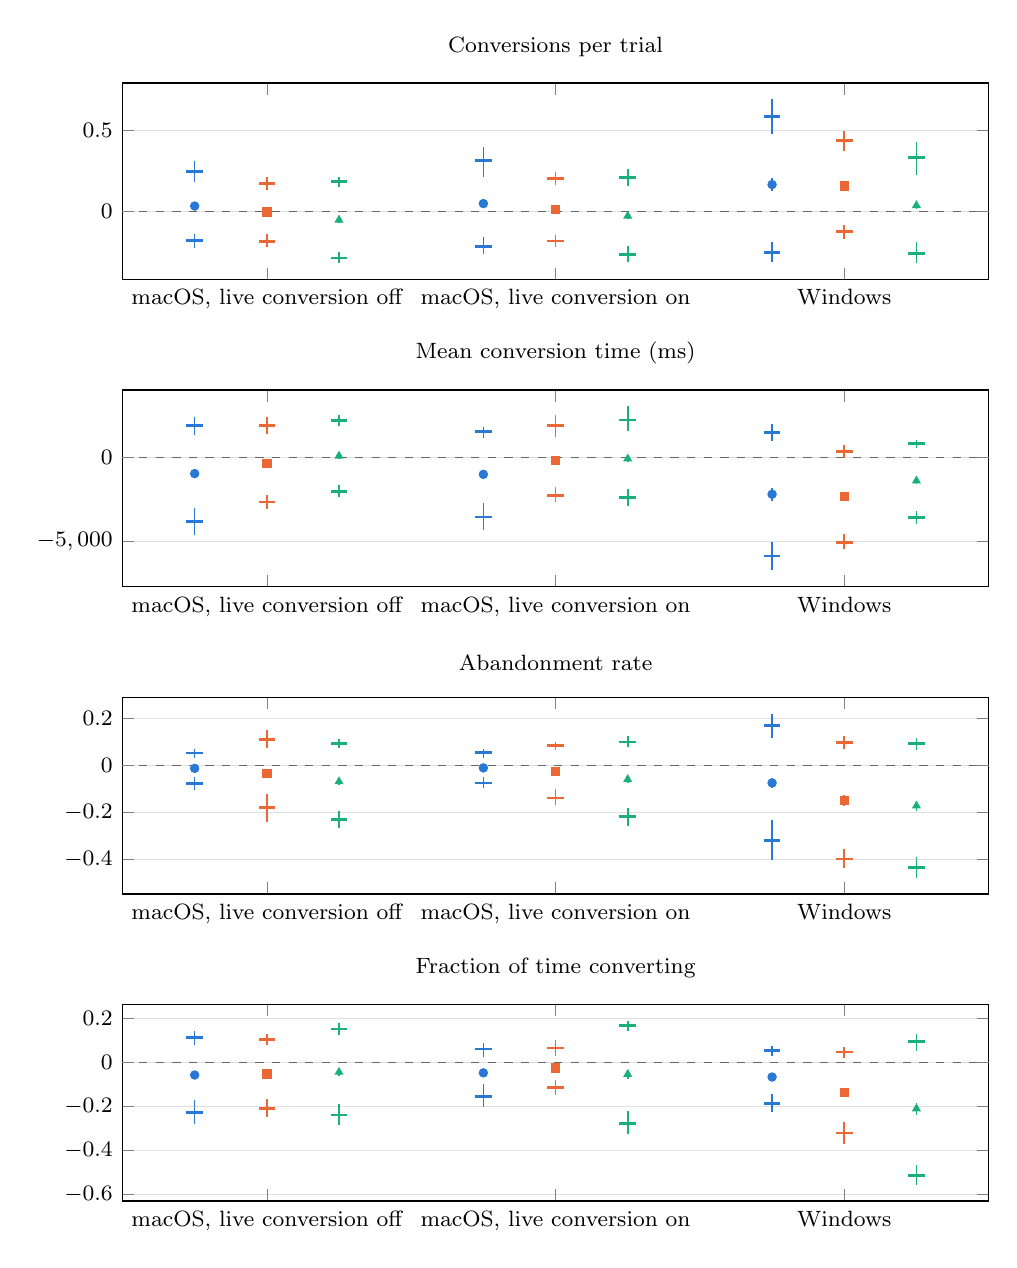
\begin{tikzpicture}
\begin{groupplot}[group style={group size=1 by 4, vertical sep=1.4cm}, fig panel, fig zero, scale only axis, width=11cm, height=2.5cm, xtick={1,2,3}, xticklabels={{macOS, live conversion off},{macOS, live conversion on},{Windows}}, xmin=0.5, xmax=3.5]
\nextgroupplot[title={Conversions per trial}, legend to name=fig:text-agreement:legend, legend columns=4]
\addlegendimage{fig slow, fig point}
\addlegendentry{slow}
\addlegendimage{fig mid, fig point}
\addlegendentry{mid}
\addlegendimage{fig fast, fig point}
\addlegendentry{fast}
\addlegendimage{black, fig limit}
\addlegendentry{limit of agreement}
\addplot[forget plot, fig interval, fig slow] table[row sep=\\] {x y\\0.75 0.0137968\\0.75 0.0565787\\0.75 nan\\0.75 -0.220809\\0.75 -0.136131\\0.75 nan\\0.75 0.179633\\0.75 0.308846\\0.75 nan\\1.75 0.0248955\\1.75 0.0760574\\1.75 nan\\1.75 -0.261969\\1.75 -0.15442\\1.75 nan\\1.75 0.215324\\1.75 0.399236\\1.75 nan\\2.75 0.127467\\2.75 0.209161\\2.75 nan\\2.75 -0.310034\\2.75 -0.187389\\2.75 nan\\2.75 0.474696\\2.75 0.690745\\2.75 nan\\};
\addplot[forget plot, fig slow, fig limit] table[row sep=\\] {x y\\0.75 -0.178767\\1.75 -0.214465\\2.75 -0.250327\\0.75 0.247509\\1.75 0.313681\\2.75 0.583864\\};
\addplot[forget plot, fig slow, fig point] table[row sep=\\] {x y\\0.75 0.0343712\\1.75 0.049608\\2.75 0.166768\\};
\addplot[forget plot, fig interval, fig mid] table[row sep=\\] {x y\\1 -0.0178577\\1 0.00922975\\1 nan\\1 -0.220274\\1 -0.137461\\1 nan\\1 0.133838\\1 0.215377\\1 nan\\2 -0.00826278\\2 0.0355079\\2 nan\\2 -0.217972\\2 -0.142543\\2 nan\\2 0.161662\\2 0.245401\\2 nan\\3 0.134052\\3 0.179142\\3 nan\\3 -0.166346\\3 -0.0797757\\3 nan\\3 0.375232\\3 0.494742\\3 nan\\};
\addplot[forget plot, fig mid, fig limit] table[row sep=\\] {x y\\1 -0.181472\\2 -0.181242\\3 -0.12198\\1 0.174879\\2 0.206037\\3 0.436799\\};
\addplot[forget plot, fig mid, fig point] table[row sep=\\] {x y\\1 -0.0032967\\2 0.0123978\\3 0.15741\\};
\addplot[forget plot, fig interval, fig fast] table[row sep=\\] {x y\\1.25 -0.0684778\\1.25 -0.0321009\\1.25 nan\\1.25 -0.318354\\1.25 -0.247791\\1.25 nan\\1.25 0.149591\\1.25 0.214642\\1.25 nan\\2.25 -0.0471251\\2.25 -0.00645323\\2.25 nan\\2.25 -0.311293\\2.25 -0.214478\\2.25 nan\\2.25 0.159809\\2.25 0.259746\\2.25 nan\\3.25 0.0132262\\3.25 0.0645655\\3.25 nan\\3.25 -0.318555\\3.25 -0.185716\\3.25 nan\\3.25 0.225438\\3.25 0.43123\\3.25 nan\\};
\addplot[forget plot, fig fast, fig limit] table[row sep=\\] {x y\\1.25 -0.28563\\2.25 -0.262432\\3.25 -0.256792\\1.25 0.18388\\2.25 0.20955\\3.25 0.333511\\};
\addplot[forget plot, fig fast, fig point] table[row sep=\\] {x y\\1.25 -0.0508751\\2.25 -0.0264411\\3.25 0.0383598\\};
\nextgroupplot[title={Mean conversion time (ms)}]
\addplot[forget plot, fig interval, fig slow] table[row sep=\\] {x y\\0.75 -1261.86\\0.75 -691.009\\0.75 nan\\0.75 -4610.86\\0.75 -3041.94\\0.75 nan\\0.75 1357.61\\0.75 2423.44\\0.75 nan\\1.75 -1287.48\\1.75 -769.965\\1.75 nan\\1.75 -4315.51\\1.75 -2725.52\\1.75 nan\\1.75 1129.49\\1.75 1824.28\\1.75 nan\\2.75 -2579.08\\2.75 -1852.1\\2.75 nan\\2.75 -6748.57\\2.75 -5032.46\\2.75 nan\\2.75 984.201\\2.75 1976.19\\2.75 nan\\};
\addplot[forget plot, fig slow, fig limit] table[row sep=\\] {x y\\0.75 -3841.17\\1.75 -3552.51\\2.75 -5878.05\\0.75 1899.84\\1.75 1523.73\\2.75 1475.88\\};
\addplot[forget plot, fig slow, fig point] table[row sep=\\] {x y\\0.75 -970.666\\1.75 -1014.39\\2.75 -2201.08\\};
\addplot[forget plot, fig interval, fig mid] table[row sep=\\] {x y\\1 -557.669\\1 -178.966\\1 nan\\1 -3073.94\\1 -2240.67\\1 nan\\1 1413.68\\1 2389.74\\1 nan\\2 -393.016\\2 45.8076\\2 nan\\2 -2690.07\\2 -1764.42\\2 nan\\2 1222.49\\2 2540.43\\2 nan\\3 -2571.92\\3 -2116.47\\3 nan\\3 -5490.45\\3 -4574.81\\3 nan\\3 -25.5713\\3 709.108\\3 nan\\};
\addplot[forget plot, fig mid, fig limit] table[row sep=\\] {x y\\1 -2662.93\\2 -2254.78\\3 -5058.22\\1 1905.33\\2 1907.89\\3 371.489\\};
\addplot[forget plot, fig mid, fig point] table[row sep=\\] {x y\\1 -378.801\\2 -173.443\\3 -2343.37\\};
\addplot[forget plot, fig interval, fig fast] table[row sep=\\] {x y\\1.25 -94.6766\\1.25 257.511\\1.25 nan\\1.25 -2338.43\\1.25 -1660.41\\1.25 nan\\1.25 1845.51\\1.25 2514.94\\1.25 nan\\2.25 -296.116\\2.25 156.763\\2.25 nan\\2.25 -2895.36\\2.25 -1883.35\\2.25 nan\\2.25 1547.61\\2.25 3036.08\\2.25 nan\\3.25 -1600.93\\3.25 -1207.2\\3.25 nan\\3.25 -3979.15\\3.25 -3198.67\\3.25 nan\\3.25 565.278\\3.25 1042.63\\3.25 nan\\};
\addplot[forget plot, fig fast, fig limit] table[row sep=\\] {x y\\1.25 -2025.32\\2.25 -2384.61\\3.25 -3604.34\\1.25 2196.62\\2.25 2221.25\\3.25 814.444\\};
\addplot[forget plot, fig fast, fig point] table[row sep=\\] {x y\\1.25 85.6454\\2.25 -81.6779\\3.25 -1394.95\\};
\nextgroupplot[title={Abandonment rate}]
\addplot[forget plot, fig interval, fig slow] table[row sep=\\] {x y\\0.75 -0.0183359\\0.75 -0.00550392\\0.75 nan\\0.75 -0.103954\\0.75 -0.0466396\\0.75 nan\\0.75 0.0339079\\0.75 0.0695433\\0.75 nan\\1.75 -0.0162794\\1.75 -0.00358063\\1.75 nan\\1.75 -0.0974907\\1.75 -0.0464943\\1.75 nan\\1.75 0.0334953\\1.75 0.0702787\\1.75 nan\\2.75 -0.0974065\\2.75 -0.0521038\\2.75 nan\\2.75 -0.404381\\2.75 -0.231365\\2.75 nan\\2.75 0.118328\\2.75 0.222407\\2.75 nan\\};
\addplot[forget plot, fig slow, fig limit] table[row sep=\\] {x y\\0.75 -0.0775651\\1.75 -0.0740273\\2.75 -0.318412\\0.75 0.0542846\\1.75 0.0546118\\2.75 0.171065\\};
\addplot[forget plot, fig slow, fig point] table[row sep=\\] {x y\\0.75 -0.0116402\\1.75 -0.0097077\\2.75 -0.0736739\\};
\addplot[forget plot, fig interval, fig mid] table[row sep=\\] {x y\\1 -0.0468264\\1 -0.0222586\\1 nan\\1 -0.238715\\1 -0.120698\\1 nan\\1 0.0736147\\1 0.149951\\1 nan\\2 -0.0372833\\2 -0.0155313\\2 nan\\2 -0.169692\\2 -0.100276\\2 nan\\2 0.0664793\\2 0.0997035\\2 nan\\3 -0.171625\\3 -0.127335\\3 nan\\3 -0.435022\\3 -0.356656\\3 nan\\3 0.0691825\\3 0.127661\\3 nan\\};
\addplot[forget plot, fig mid, fig limit] table[row sep=\\] {x y\\1 -0.178358\\2 -0.13783\\3 -0.398436\\1 0.110083\\2 0.0856654\\3 0.0987183\\};
\addplot[forget plot, fig mid, fig point] table[row sep=\\] {x y\\1 -0.0341372\\2 -0.0260823\\3 -0.149859\\};
\addplot[forget plot, fig interval, fig fast] table[row sep=\\] {x y\\1.25 -0.0808639\\1.25 -0.0554578\\1.25 nan\\1.25 -0.266532\\1.25 -0.1935\\1.25 nan\\1.25 0.0736502\\1.25 0.113685\\1.25 nan\\2.25 -0.0728879\\2.25 -0.0449424\\2.25 nan\\2.25 -0.256723\\2.25 -0.180276\\2.25 nan\\2.25 0.0787637\\2.25 0.124625\\2.25 nan\\3.25 -0.192895\\3.25 -0.148815\\3.25 nan\\3.25 -0.477632\\3.25 -0.389368\\3.25 nan\\3.25 0.0663391\\3.25 0.118487\\3.25 nan\\};
\addplot[forget plot, fig fast, fig limit] table[row sep=\\] {x y\\1.25 -0.230252\\2.25 -0.217832\\3.25 -0.436111\\1.25 0.0948428\\2.25 0.101054\\3.25 0.0937557\\};
\addplot[forget plot, fig fast, fig point] table[row sep=\\] {x y\\1.25 -0.0677045\\2.25 -0.058389\\3.25 -0.171178\\};
\nextgroupplot[title={Fraction of time converting}]
\addplot[forget plot, fig interval, fig slow] table[row sep=\\] {x y\\0.75 -0.0727727\\0.75 -0.0419352\\0.75 nan\\0.75 -0.278801\\0.75 -0.16807\\0.75 nan\\0.75 0.0801202\\0.75 0.14193\\0.75 nan\\1.75 -0.0583606\\1.75 -0.0365913\\1.75 nan\\1.75 -0.203414\\1.75 -0.0991124\\1.75 nan\\1.75 0.0236671\\1.75 0.0902096\\1.75 nan\\2.75 -0.0757142\\2.75 -0.0555747\\2.75 nan\\2.75 -0.223332\\2.75 -0.144563\\2.75 nan\\2.75 0.0279813\\2.75 0.0763184\\2.75 nan\\};
\addplot[forget plot, fig slow, fig limit] table[row sep=\\] {x y\\0.75 -0.226043\\1.75 -0.15533\\2.75 -0.18638\\0.75 0.113162\\1.75 0.062031\\2.75 0.0552155\\};
\addplot[forget plot, fig slow, fig point] table[row sep=\\] {x y\\0.75 -0.0564405\\1.75 -0.0466495\\2.75 -0.0655823\\};
\addplot[forget plot, fig interval, fig mid] table[row sep=\\] {x y\\1 -0.0647352\\1 -0.037892\\1 nan\\1 -0.24751\\1 -0.166924\\1 nan\\1 0.0818906\\1 0.129647\\1 nan\\2 -0.0310215\\2 -0.0169641\\2 nan\\2 -0.148586\\2 -0.0769847\\2 nan\\2 0.0300855\\2 0.101428\\2 nan\\3 -0.156174\\3 -0.116918\\3 nan\\3 -0.369001\\3 -0.270129\\3 nan\\3 0.0200337\\3 0.0721026\\3 nan\\};
\addplot[forget plot, fig mid, fig limit] table[row sep=\\] {x y\\1 -0.209188\\2 -0.114821\\3 -0.320378\\1 0.107008\\2 0.0667371\\3 0.0483024\\};
\addplot[forget plot, fig mid, fig point] table[row sep=\\] {x y\\1 -0.0510901\\2 -0.0240419\\3 -0.136038\\};
\addplot[forget plot, fig interval, fig fast] table[row sep=\\] {x y\\1.25 -0.0598186\\1.25 -0.0271184\\1.25 nan\\1.25 -0.28509\\1.25 -0.187262\\1.25 nan\\1.25 0.124557\\1.25 0.181799\\1.25 nan\\2.25 -0.074464\\2.25 -0.0333915\\2.25 nan\\2.25 -0.323565\\2.25 -0.22158\\2.25 nan\\2.25 0.145255\\2.25 0.191593\\2.25 nan\\3.25 -0.238401\\3.25 -0.181827\\3.25 nan\\3.25 -0.556206\\3.25 -0.468247\\3.25 nan\\3.25 0.0544072\\3.25 0.129845\\3.25 nan\\};
\addplot[forget plot, fig fast, fig limit] table[row sep=\\] {x y\\1.25 -0.23921\\2.25 -0.275999\\3.25 -0.514636\\1.25 0.153092\\2.25 0.170183\\3.25 0.0950716\\};
\addplot[forget plot, fig fast, fig point] table[row sep=\\] {x y\\1.25 -0.043059\\2.25 -0.0529079\\3.25 -0.209782\\};
\end{groupplot}
\end{tikzpicture}
\caption{Per-text agreement of the four measures per cell and speed in the primary scope: the bias (marks) and the lower and upper limits of agreement (dashes) of the per-text difference (observation minus reference), each with a 95\% interval that resamples blocks. The values hold for this design's numbers of trials per text and are not compared between speeds, and the values of the Windows cell estimate the agreement with a different construct and are not compared with those of the macOS cells; a measure with no text in the scope is not drawn. Table~\ref{tab:text-agreement} gives the values with ICC(A,1). The figure is drawn from the result files by code written and reviewed with an AI tool (Claude) and checked by its tests; see the AI declaration}
\label{fig:text-agreement}
\end{figure}


% Section 8 of the manuscript: text recoverability (question 4). The method is stated first, as the outline
% requires; it follows sections 6.8 and 10.7 of the frozen registration. The results are written from the result
% files e2_closed_set_<cell>.json and e2_open_set_<cell>.json after the analysis.

\section{Results: text recoverability}
\label{sec:recoverability}

\subsection{Method}
\label{sec:recoverability-method}

The text-recoverability study asked how much of the typed text the key rows of a published log still reveal. Two
attacks were run on the observation log of each cell separately, with the plan, the procedures and the settings that
built it; the attacks refused a log whose plan or settings did not match. Both read the category and the time of
every key row of a press and nothing else: they did not use the session rows or the rows of key releases, and no plan
sent a modifier key, so on Windows, where modifier keys produce rows, no such row was read either. The ground truth of
an attack was the reading that was typed,
not the original sentence. The trials of scenario S12, whose phrase is a generated kana string, were not scored. When
every block is scored this leaves 2{,}925 trials with live conversion on and 2{,}700 with it off on macOS, and 2{,}700
on Windows.

\paragraph{Assigning presses to trials.} Both attacks assign the observed presses to the trials in plan order, block
by block. A block is placed where its marker of four arrow presses and all its trials match the observed presses. A
block whose observed presses do not agree with the plan (a press missing, added or changed) is not scored: its trials
are counted as unscored, and the assignment continues with the next block that matches, so that a difference loses
only the block that holds it. This behaviour was checked by the self-test of the code on the cases it constructs, not
proved in general. Before each freeze the assignment, without any attack, was run on the key rows of the pilots: it
scored every block of the three macOS pilot runs that used the arrow-key marker (15 blocks, 282 trials) and of the
seven Windows pilot runs (27 blocks, 429 trials) and left no press unassigned. These logs had no missing or added
press, so the check shows that clean logs are scored whole; it does not exercise the recovery after a difference.
Accuracies and error rates are computed over the scored trials, and the numbers of unscored blocks and trials are
reported per cell.

\paragraph{Closed set.} For each trial the attacker was given $K$ candidate phrases, the true one and $K-1$ decoys
drawn from the phrases that the trial's scenario could have produced (excluding phrases with the same reading). It
knew the scenario, the system, the speed, the generator, the procedures and the settings, generated the expected log
of each candidate with the same generator, and chose the candidate whose expected log was closest to the observed
one. $K$ was 10, 100 and 1{,}000. The attack was repeated on six feature sets that remove information from the log,
named here, in the figures and in the tables as in the registration: exact times (\texttt{all}), no times
(\texttt{no\_time}), times in 1-second bins (\texttt{bin1s}), and each of these three with every run of letter keys
made one token (\texttt{no\_runs}, \texttt{bin1s\_count} and \texttt{counts\_only}). The registration describes the
last three as having no lengths of letter runs, but the token of a run kept the number of its presses, and the distance
charged the difference of these numbers; what the three sets removed was the time of every press of a run after its
first (deviation D13). Without times, \texttt{counts\_only} therefore held the same information as \texttt{no\_time},
the category of every press in order, and differed from it only in how the distance counted a run of letter keys.
Because an attacker given a detailed log can always discard
information, the accuracy of a feature set is the maximum over that set and every coarser set derived from it. The
accuracy is reported with its Wilson interval and, descriptively, with a 95\% percentile interval from 2{,}000
resamples of whole blocks, together with the chance level $1/K$, the mean rank of the true phrase and, without an
interval, the accuracy of each feature set alone per scenario and per speed.

\paragraph{The near-chance rule.} The synthetic key intervals were drawn independently of the keys, so the logs carry
none of the timing structure of human typing, neither the timing of particular key pairs nor the pauses between words
and phrases. The accuracy on the four feature sets that keep any time is therefore reported as an estimate only and
does not enter the recommendation, which considers the two sets that keep no time (\texttt{no\_time} and
\texttt{counts\_only}, registered as its coarsening). The accuracy of a feature set is near chance at $K=10$ or $K=100$
when the upper
end of its 95\% Wilson interval is at most $2/K$. A set is near chance for the recommendation when it is near chance at
both values of $K$ in both macOS cells, and the recommended granularity is the more detailed of the two sets that is
near chance in this sense; if neither is, no granularity is recommended, and this is reported. At $K=1{,}000$ an attack
at the chance level would rarely be judged near chance at the planned numbers of trials, so $K=1{,}000$ is reported
descriptively and is not part of the rule. The probability of the judgement at the planned numbers of trials was fixed
in the registration and is given with the results (Table~\ref{tab:nearchance}). The margin of $2/K$ and the values of
$K$ are choices of the design, not derived from a criterion of privacy. The Wilson interval treats trials as
independent; with positive dependence within a block the rule can be met more easily than it should be, which is why the
block-resampled interval is reported next to it. The recommendation was decided from the two macOS cells. The same
judgement was made for the Windows cell and, where it does not hold, is reported as a qualification of the
recommendation for logs recorded on Windows; it does not change the recommendation.

\paragraph{Exploratory: feature sets without run lengths.} Because no registered set dropped the lengths of letter
runs, the closed-set attack was also run, as an exploratory analysis that is not registered (deviation D13), on two
feature sets without times that drop them: \texttt{letter\_runs\_unit}, in which every run of letter keys is one token
whatever its length and every other press one token, and \texttt{all\_runs\_unit}, in which every run of presses of the
same category is one token whatever its length, so that the numbers of Backspace, arrow and other repeated presses are
dropped as well. Both keep the order of the tokens. The predicted logs, the distance, the candidates and the
tie-breaking of each trial, the values of $K$ and the intervals were those of the registered attack, and every run also
computed \texttt{no\_time} and \texttt{counts\_only} and stopped unless they equalled the registered results. As
\texttt{all\_runs\_unit} can be derived from \texttt{letter\_runs\_unit}, the accuracy of \texttt{letter\_runs\_unit}
is the larger of the two. Both sets can also be derived from \texttt{no\_time} and \texttt{counts\_only}; at every $K$
and in every cell each was less accurate than both, so the registered accuracies, their Wilson intervals and the
registered judgement are unchanged. The registered near-chance rule was applied to both sets as an exploratory judgement, from
the two macOS cells, with the Windows judgement as its qualification; it is reported next to the registered judgement
and does not change the recommendation. The two sets, the rule and the place of the result in this article were fixed
after all registered results had been seen and before the analysis was run, and a related measurement on single trials
of the Windows cell, made with a related attack in another study, had been seen before (deviation D13).

\paragraph{Open set.} A second attacker saw only the categories of the key presses and, with a character language
model, searched for the kana string that Romaji input would spell with exactly the observed letter keys and the
observed punctuation, maximising its probability. Two levels of knowledge were evaluated, named K0 and K1 as in the
registration (the names are not the number $K$ of candidates of the closed set). K0 knew nothing of the genre beyond
the frequency of single characters (a character unigram model estimated from the training phrases). K1 knew the
genre but not the individual work: a character trigram model with Witten--Bell smoothing
\citep{wittenbell1991}, trained on the corpus with the whole works of the evaluation phrases held out (three of the
twelve works, drawn with the seed, holding at least a fifth of the phrases; a training phrase with the reading of an
evaluation phrase was removed). A stronger attacker of the second level, K1+, for which the corpus was split by phrase
instead of by work, is reported alongside it. The baseline was the same model without the log, drawing a string from
its prior while knowing either the number of segments or the true length. Reported are the character error rate of
the attack and of the baseline, their paired difference, and the difference from a negative control in which each
trial is decoded from another trial's observation, each with a percentile interval from resampling whole blocks. The
open set does not enter the rule; it is reported next to the recommendation as a second view of what the lengths of
letter runs, which the \texttt{no\_time} set keeps, reveal.

\paragraph{What is not evaluated.} The rule judges the identification of one phrase among $K$ candidates in one
trial; it is not a criterion of privacy. Combining several trials of one writer, matching a log against known final
texts, and identifying a writer from the timing of a log are not evaluated, and no log is described as safe to
publish. The session rows carry their
times and durations in milliseconds and could undo the coarsening of the key rows; they were not given to the attacks,
and publishing them is not evaluated. Neither are the rows of key releases or, on Windows, the rows of modifier keys.
The feature sets that keep time are reported as estimates only, so whether key rows with times can be published is
not judged, and granularities between milliseconds and 1-second bins were not evaluated. Neither attack is
claimed to be the strongest possible. The attacker knew the generator and the procedures, and the input had no
typing errors; these conditions are expected to favour identification, which is stated as an expectation, not as a
result.

\subsection{Results}
\label{sec:recoverability-results}

Every block of every cell was scored (\rv{macos-standard-live-off.q4.unscored} unscored with live conversion off,
\rv{macos-standard-live-on.q4.unscored} with it on, \rv{windows-msime-tsf.q4.unscored} on Windows), so the rule was
applied to the planned numbers of trials, whose properties Table~\ref{tab:nearchance} gives.

\paragraph{Closed set and the recommendation.} Table~\ref{tab:closed-set} gives the accuracy of the two feature sets
that keep no time. With live conversion off, the accuracy of \texttt{no\_time} was
\rv{macos-standard-live-off.q4.no_time.k10.acc} at $K = 10$ and \rv{macos-standard-live-off.q4.no_time.k100.acc} at
$K = 100$; with it on, \rv{macos-standard-live-on.q4.no_time.k10.acc} and
\rv{macos-standard-live-on.q4.no_time.k100.acc}. The accuracy of \texttt{counts\_only}, the coarsest registered set,
from which no other registered set is derived, was \rv{macos-standard-live-off.q4.counts_only.k10.acc} and
\rv{macos-standard-live-off.q4.counts_only.k100.acc} with live conversion off and
\rv{macos-standard-live-on.q4.counts_only.k10.acc} and \rv{macos-standard-live-on.q4.counts_only.k100.acc} with it on.
In both macOS cells the upper end of every one of these Wilson intervals lies above $2/K$, so neither set is near chance
under the registered rule, which is not a criterion of privacy (Section~\ref{sec:recoverability-method};
\texttt{no\_time}: \rv{macos-standard-live-off.q4.no_time.near} and
\rv{macos-standard-live-on.q4.no_time.near}; \texttt{counts\_only}: \rv{macos-standard-live-off.q4.counts_only.near}
and \rv{macos-standard-live-on.q4.counts_only.near}), and the recommended granularity is \rv{q4.recommendation}: no
granularity of the key rows is recommended. In both macOS cells, at $K = 10$ and $K = 100$, the
maximum that gives the accuracy of \texttt{no\_time} came from the attack on \texttt{counts\_only}, which holds the
same information as \texttt{no\_time} and differs from it only in how its distance counts a run of letter keys
(Section~\ref{sec:recoverability-method}): counted as one token of its length, the runs identified the phrase at least
as often as the attack on \texttt{no\_time} alone did (supplement). The decoys were drawn from the phrases of the
trial's scenario, whose readings have 6 to 30 kana (Section~\ref{sec:method-plans}), and were not matched to the true
phrase in length.

On Windows, under the same judgement, \rv{q4.windows.qualification}. The Windows accuracies of the two sets equal those
of the macOS cell with live conversion off to the reported precision. The two plans were generated from the same seed
and share every trial's block, scenario, speed, phrase and times; their presses differ only in S2, where the macOS
procedure presses one Return more, and in S4, where the Windows procedure presses one Escape more (deviation D1), and
the presses of letters, digits and punctuation are the same in every trial. The Windows judgement is therefore not an
independent replication of the macOS one for these sets.

% Every word of the exploratory judgement is generated from the result files (q4x.*); the paragraph was to be here
% whatever the result (deviation D13).
\paragraph{Exploratory: feature sets without run lengths.} In the exploratory analysis of deviation D13, the accuracy of
\texttt{letter\_runs\_unit} was \rv{macos-standard-live-off.q4x.letter_runs_unit.k10.acc} at $K = 10$ and
\rv{macos-standard-live-off.q4x.letter_runs_unit.k100.acc} at $K = 100$ with live conversion off and
\rv{macos-standard-live-on.q4x.letter_runs_unit.k10.acc} and \rv{macos-standard-live-on.q4x.letter_runs_unit.k100.acc}
with it on; that of \texttt{all\_runs\_unit}, which also drops the numbers of repeated presses of the other categories,
was \rv{macos-standard-live-off.q4x.all_runs_unit.k10.acc} and \rv{macos-standard-live-off.q4x.all_runs_unit.k100.acc}
with live conversion off and \rv{macos-standard-live-on.q4x.all_runs_unit.k10.acc} and
\rv{macos-standard-live-on.q4x.all_runs_unit.k100.acc} with it on. Under the registered rule, applied as an exploratory
judgement, \rv{q4x.judgement}: in both cells, \rv{q4x.byk} (\texttt{letter\_runs\_unit} with live conversion off
and on: \rv{macos-standard-live-off.q4x.letter_runs_unit.k10.near} and
\rv{macos-standard-live-on.q4x.letter_runs_unit.k10.near} at $K = 10$,
\rv{macos-standard-live-off.q4x.letter_runs_unit.k100.near} and
\rv{macos-standard-live-on.q4x.letter_runs_unit.k100.near} at $K = 100$; \texttt{all\_runs\_unit}:
\rv{macos-standard-live-off.q4x.all_runs_unit.k10.near} and \rv{macos-standard-live-on.q4x.all_runs_unit.k10.near},
\rv{macos-standard-live-off.q4x.all_runs_unit.k100.near} and \rv{macos-standard-live-on.q4x.all_runs_unit.k100.near}).
Applied to these two sets, the rule would recommend \rv{q4x.granularity}. On Windows, under the same judgement,
\rv{q4x.windows}; as for the registered sets, its values equal those of the macOS cell with live conversion off. The
registered judgement and recommendation do not change. The supplement gives both sets at every $K$, with the accuracy
per speed and per scenario.

Figure~\ref{fig:closed-set} shows every feature set at every $K$, and the supplement gives their values, with the
accuracy per speed and scenario. The sets that keep time are estimates only and enter neither the judgement nor the
recommendation (Section~\ref{sec:recoverability-method}). The accuracy of an attack on a set alone was not monotone in
the information the set keeps: at $K = 10$ the attack on \texttt{all} alone identified fewer phrases than the attack on
\texttt{counts\_only} in both macOS cells (supplement), so the attacks are not the strongest possible, and the maximum
over the coarser sets is what the figure shows.

\paragraph{Open set.} Table~\ref{tab:open-set} gives the character error rate of the attack and of the prior-only
baseline, their difference (gain), and the gain over the shuffled control, in which each trial is decoded from another
trial's observation. With the number of segments known, the gain of K1 was
\rv{macos-standard-live-off.q4.open.K1.count.gain} with live conversion off and
\rv{macos-standard-live-on.q4.open.K1.count.gain} with it on, and its gain over the shuffled control
\rv{macos-standard-live-off.q4.open.K1.count.gainvsshuffled} and
\rv{macos-standard-live-on.q4.open.K1.count.gainvsshuffled}; for K1+ the gain over the shuffled control was
\rv{macos-standard-live-off.q4.open.K1plus.count.gainvsshuffled} and
\rv{macos-standard-live-on.q4.open.K1plus.count.gainvsshuffled}, and for K0
\rv{macos-standard-live-off.q4.open.K0.count.gainvsshuffled} and
\rv{macos-standard-live-on.q4.open.K0.count.gainvsshuffled}. With the true length known, the gain of K1 over the
baseline was \rv{macos-standard-live-off.q4.open.K1.true.gain} and \rv{macos-standard-live-on.q4.open.K1.true.gain}. The
open-set file of the Windows cell is byte-identical to that of the macOS cell with live conversion off: the attack
decodes the letter keys and the punctuation, which the two plans share, and every press other than the input-mode keys
reached the log in both cells. The open set does not enter the rule; it is a second view of what the letter-run lengths
kept by \texttt{no\_time} reveal, for these attacks.

% Generated by manuscript/tools/results_tables.py from the result files; do not edit by hand.
\begin{sidewaystable}[p]
\caption{Closed-set identification for the two feature sets that keep no time: the accuracy (the maximum over the set and the sets derivable from it) with its Wilson interval and, descriptively, the interval that resamples blocks; a set is near chance at K when the upper end of the Wilson interval is at most 2/K, and near chance for the rule when it is so at both K = 10 and K = 100. The recommendation is decided from the two macOS cells; the Windows judgement is reported as its qualification; --: no value}
\label{tab:closed-set}
\begin{tabular}{L{0.20}L{0.12}L{0.06}L{0.07}L{0.22}L{0.15}L{0.07}L{0.10}}
\toprule
Cell & Feature set & K & Trials & Accuracy & Block interval & 2/K & Near chance \\
\midrule
macOS, live conversion off & \texttt{no\_time} & 10 & 2{,}700 & 0.902 [0.890, 0.913] & 0.891, 0.913 & 0.200 & no \\
 & \texttt{no\_time} & 100 & 2{,}700 & 0.421 [0.403, 0.440] & 0.408, 0.442 & 0.020 & no \\
 & \texttt{counts\_only} & 10 & 2{,}700 & 0.902 [0.890, 0.913] & 0.890, 0.913 & 0.200 & no \\
 & \texttt{counts\_only} & 100 & 2{,}700 & 0.421 [0.403, 0.440] & 0.403, 0.440 & 0.020 & no \\
macOS, live conversion on & \texttt{no\_time} & 10 & 2{,}925 & 0.907 [0.896, 0.917] & 0.897, 0.917 & 0.200 & no \\
 & \texttt{no\_time} & 100 & 2{,}925 & 0.435 [0.417, 0.453] & 0.418, 0.454 & 0.020 & no \\
 & \texttt{counts\_only} & 10 & 2{,}925 & 0.907 [0.896, 0.917] & 0.896, 0.917 & 0.200 & no \\
 & \texttt{counts\_only} & 100 & 2{,}925 & 0.435 [0.417, 0.453] & 0.417, 0.453 & 0.020 & no \\
Windows & \texttt{no\_time} & 10 & 2{,}700 & 0.902 [0.890, 0.913] & 0.891, 0.913 & 0.200 & no \\
 & \texttt{no\_time} & 100 & 2{,}700 & 0.421 [0.403, 0.440] & 0.408, 0.442 & 0.020 & no \\
 & \texttt{counts\_only} & 10 & 2{,}700 & 0.902 [0.890, 0.913] & 0.890, 0.913 & 0.200 & no \\
 & \texttt{counts\_only} & 100 & 2{,}700 & 0.421 [0.403, 0.440] & 0.403, 0.440 & 0.020 & no \\
\midrule
\multicolumn{8}{l}{Recommendation from the two macOS cells: none} \\
\bottomrule
\end{tabular}
\end{sidewaystable}

% Generated by manuscript/tools/results_tables.py from the result files; do not edit by hand.
\begin{figure}[t]
\centering
\pgfplotslegendfromname{fig:closed-set:legend}\par\medskip
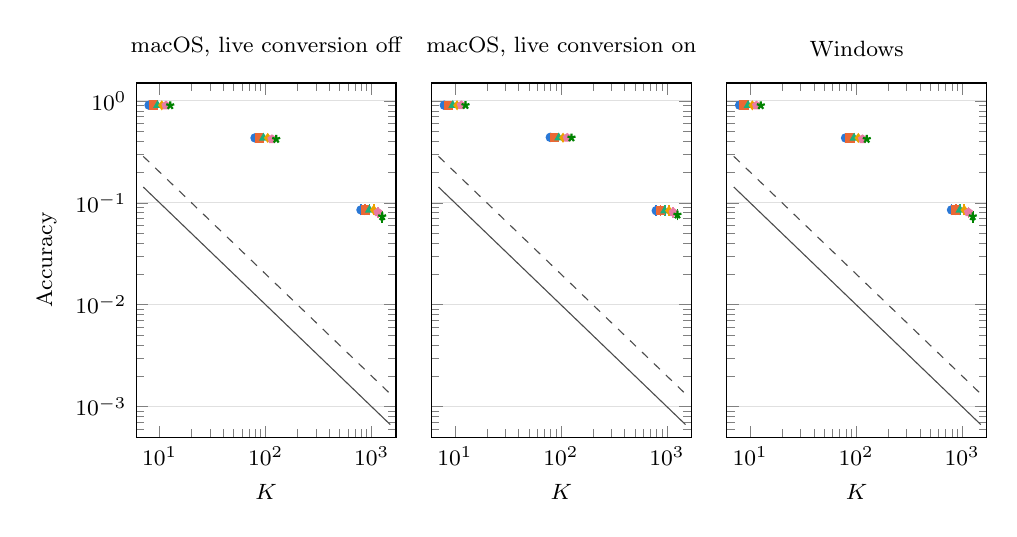
\begin{tikzpicture}
\begin{groupplot}[group style={group size=3 by 1, horizontal sep=0.45cm, yticklabels at=edge left, ylabels at=edge left}, fig panel, xmode=log, ymode=log, xtick={10,100,1000}, xmin=6, xmax=1700, ymin=0.0005, ymax=1.5, scale only axis, width=3.3cm, height=4.5cm, xlabel={$K$}, ylabel={Accuracy}]
\nextgroupplot[title={macOS, live conversion off}, legend to name=fig:closed-set:legend, legend columns=4]
\addlegendimage{fig set1, fig point}
\addlegendentry{\texttt{all}}
\addlegendimage{fig set2, fig point}
\addlegendentry{\texttt{no\_runs}}
\addlegendimage{fig set3, fig point}
\addlegendentry{\texttt{bin1s}}
\addlegendimage{fig set4, fig point}
\addlegendentry{\texttt{bin1s\_count}}
\addlegendimage{fig set5, fig point}
\addlegendentry{\texttt{no\_time}}
\addlegendimage{fig set6, fig point}
\addlegendentry{\texttt{counts\_only}}
\addlegendimage{fig chance}
\addlegendentry{$1/K$}
\addlegendimage{fig margin}
\addlegendentry{$2/K$}
\addplot[forget plot, fig chance, domain=7:1500] {1/x};
\addplot[forget plot, fig margin, domain=7:1500] {2/x};
\addplot[forget plot, fig interval, fig set1] table[row sep=\\] {x y\\7.94328 0.897056\\7.94328 0.91882\\7.94328 nan\\79.4328 0.41475\\79.4328 0.452106\\79.4328 nan\\794.328 0.0752358\\794.328 0.0963132\\794.328 nan\\};
\addplot[forget plot, fig set1, fig point] table[row sep=\\] {x y\\7.94328 0.908519\\79.4328 0.433333\\794.328 0.0851852\\};
\addplot[forget plot, fig interval, fig set2] table[row sep=\\] {x y\\8.70964 0.897056\\8.70964 0.91882\\8.70964 nan\\87.0964 0.41475\\87.0964 0.452106\\87.0964 nan\\870.964 0.0752358\\870.964 0.0963132\\870.964 nan\\};
\addplot[forget plot, fig set2, fig point] table[row sep=\\] {x y\\8.70964 0.908519\\87.0964 0.433333\\870.964 0.0851852\\};
\addplot[forget plot, fig interval, fig set3] table[row sep=\\] {x y\\9.54993 0.893163\\9.54993 0.915316\\9.54993 nan\\95.4993 0.41475\\95.4993 0.452106\\95.4993 nan\\954.993 0.0752358\\954.993 0.0963132\\954.993 nan\\};
\addplot[forget plot, fig set3, fig point] table[row sep=\\] {x y\\9.54993 0.904815\\95.4993 0.433333\\954.993 0.0851852\\};
\addplot[forget plot, fig interval, fig set4] table[row sep=\\] {x y\\10.4713 0.893163\\10.4713 0.915316\\10.4713 nan\\104.713 0.41475\\104.713 0.452106\\104.713 nan\\1047.13 0.0752358\\1047.13 0.0963132\\1047.13 nan\\};
\addplot[forget plot, fig set4, fig point] table[row sep=\\] {x y\\10.4713 0.904815\\104.713 0.433333\\1047.13 0.0851852\\};
\addplot[forget plot, fig interval, fig set5] table[row sep=\\] {x y\\11.4815 0.890052\\11.4815 0.91251\\11.4815 nan\\114.815 0.40298\\114.815 0.440206\\114.815 nan\\1148.15 0.0710503\\1148.15 0.0916225\\1148.15 nan\\};
\addplot[forget plot, fig set5, fig point] table[row sep=\\] {x y\\11.4815 0.901852\\114.815 0.421481\\1148.15 0.0807407\\};
\addplot[forget plot, fig interval, fig set6] table[row sep=\\] {x y\\12.5893 0.890052\\12.5893 0.91251\\12.5893 nan\\125.893 0.40298\\125.893 0.440206\\125.893 nan\\1258.93 0.064095\\1258.93 0.083784\\1258.93 nan\\};
\addplot[forget plot, fig set6, fig point] table[row sep=\\] {x y\\12.5893 0.901852\\125.893 0.421481\\1258.93 0.0733333\\};
\nextgroupplot[title={macOS, live conversion on}]
\addplot[forget plot, fig chance, domain=7:1500] {1/x};
\addplot[forget plot, fig margin, domain=7:1500] {2/x};
\addplot[forget plot, fig interval, fig set1] table[row sep=\\] {x y\\7.94328 0.895585\\7.94328 0.916682\\7.94328 nan\\79.4328 0.421082\\79.4328 0.457027\\79.4328 nan\\794.328 0.0742589\\794.328 0.0943543\\794.328 nan\\};
\addplot[forget plot, fig set1, fig point] table[row sep=\\] {x y\\7.94328 0.906667\\79.4328 0.438974\\794.328 0.0837607\\};
\addplot[forget plot, fig interval, fig set2] table[row sep=\\] {x y\\8.70964 0.895585\\8.70964 0.916682\\8.70964 nan\\87.0964 0.421082\\87.0964 0.457027\\87.0964 nan\\870.964 0.0742589\\870.964 0.0943543\\870.964 nan\\};
\addplot[forget plot, fig set2, fig point] table[row sep=\\] {x y\\8.70964 0.906667\\87.0964 0.438974\\870.964 0.0837607\\};
\addplot[forget plot, fig interval, fig set3] table[row sep=\\] {x y\\9.54993 0.895585\\9.54993 0.916682\\9.54993 nan\\95.4993 0.417343\\95.4993 0.453254\\95.4993 nan\\954.993 0.0742589\\954.993 0.0943543\\954.993 nan\\};
\addplot[forget plot, fig set3, fig point] table[row sep=\\] {x y\\9.54993 0.906667\\95.4993 0.435214\\954.993 0.0837607\\};
\addplot[forget plot, fig interval, fig set4] table[row sep=\\] {x y\\10.4713 0.895585\\10.4713 0.916682\\10.4713 nan\\104.713 0.417343\\104.713 0.453254\\104.713 nan\\1047.13 0.0742589\\1047.13 0.0943543\\1047.13 nan\\};
\addplot[forget plot, fig set4, fig point] table[row sep=\\] {x y\\10.4713 0.906667\\104.713 0.435214\\1047.13 0.0837607\\};
\addplot[forget plot, fig interval, fig set5] table[row sep=\\] {x y\\11.4815 0.895585\\11.4815 0.916682\\11.4815 nan\\114.815 0.417343\\114.815 0.453254\\114.815 nan\\1148.15 0.071355\\1148.15 0.0911124\\1148.15 nan\\};
\addplot[forget plot, fig set5, fig point] table[row sep=\\] {x y\\11.4815 0.906667\\114.815 0.435214\\1148.15 0.0806838\\};
\addplot[forget plot, fig interval, fig set6] table[row sep=\\] {x y\\12.5893 0.895585\\12.5893 0.916682\\12.5893 nan\\125.893 0.417343\\125.893 0.453254\\125.893 nan\\1258.93 0.067168\\1258.93 0.0864222\\1258.93 nan\\};
\addplot[forget plot, fig set6, fig point] table[row sep=\\] {x y\\12.5893 0.906667\\125.893 0.435214\\1258.93 0.0762393\\};
\nextgroupplot[title={Windows}]
\addplot[forget plot, fig chance, domain=7:1500] {1/x};
\addplot[forget plot, fig margin, domain=7:1500] {2/x};
\addplot[forget plot, fig interval, fig set1] table[row sep=\\] {x y\\7.94328 0.897056\\7.94328 0.91882\\7.94328 nan\\79.4328 0.414382\\79.4328 0.451735\\79.4328 nan\\794.328 0.0752358\\794.328 0.0963132\\794.328 nan\\};
\addplot[forget plot, fig set1, fig point] table[row sep=\\] {x y\\7.94328 0.908519\\79.4328 0.432963\\794.328 0.0851852\\};
\addplot[forget plot, fig interval, fig set2] table[row sep=\\] {x y\\8.70964 0.897056\\8.70964 0.91882\\8.70964 nan\\87.0964 0.414382\\87.0964 0.451735\\87.0964 nan\\870.964 0.0752358\\870.964 0.0963132\\870.964 nan\\};
\addplot[forget plot, fig set2, fig point] table[row sep=\\] {x y\\8.70964 0.908519\\87.0964 0.432963\\870.964 0.0851852\\};
\addplot[forget plot, fig interval, fig set3] table[row sep=\\] {x y\\9.54993 0.893163\\9.54993 0.915316\\9.54993 nan\\95.4993 0.414382\\95.4993 0.451735\\95.4993 nan\\954.993 0.0752358\\954.993 0.0963132\\954.993 nan\\};
\addplot[forget plot, fig set3, fig point] table[row sep=\\] {x y\\9.54993 0.904815\\95.4993 0.432963\\954.993 0.0851852\\};
\addplot[forget plot, fig interval, fig set4] table[row sep=\\] {x y\\10.4713 0.893163\\10.4713 0.915316\\10.4713 nan\\104.713 0.414382\\104.713 0.451735\\104.713 nan\\1047.13 0.0752358\\1047.13 0.0963132\\1047.13 nan\\};
\addplot[forget plot, fig set4, fig point] table[row sep=\\] {x y\\10.4713 0.904815\\104.713 0.432963\\1047.13 0.0851852\\};
\addplot[forget plot, fig interval, fig set5] table[row sep=\\] {x y\\11.4815 0.890052\\11.4815 0.91251\\11.4815 nan\\114.815 0.40298\\114.815 0.440206\\114.815 nan\\1148.15 0.0710503\\1148.15 0.0916225\\1148.15 nan\\};
\addplot[forget plot, fig set5, fig point] table[row sep=\\] {x y\\11.4815 0.901852\\114.815 0.421481\\1148.15 0.0807407\\};
\addplot[forget plot, fig interval, fig set6] table[row sep=\\] {x y\\12.5893 0.890052\\12.5893 0.91251\\12.5893 nan\\125.893 0.40298\\125.893 0.440206\\125.893 nan\\1258.93 0.064095\\1258.93 0.083784\\1258.93 nan\\};
\addplot[forget plot, fig set6, fig point] table[row sep=\\] {x y\\12.5893 0.901852\\125.893 0.421481\\1258.93 0.0733333\\};
\end{groupplot}
\end{tikzpicture}
\caption{Closed-set identification accuracy against the number of candidates $K$ for the six feature sets, per cell, with 95\% Wilson intervals; the accuracy of a set is the maximum over the set and the sets derivable from it. Solid line: the chance level $1/K$; dashed line: the margin $2/K$ of the near-chance rule, which judges \texttt{no\_time} and \texttt{counts\_only} at $K = 10$ and $100$; the sets that keep time are estimates only. The sets are set apart along $K$ for legibility; every point lies at $K = 10$, $100$ or $1{,}000$. Both axes are logarithmic. Table~\ref{tab:closed-set} gives the judgement. The figure is drawn from the result files by code written and reviewed with an AI tool (Claude) and checked by its tests; see the AI declaration}
\label{fig:closed-set}
\end{figure}

% Generated by manuscript/tools/results_tables.py from the result files; do not edit by hand.
\begin{sidewaystable}[p]
{\footnotesize
\caption{Open-set reconstruction per cell and attacker: character error rate (CER) of the attack and of the prior-only baseline, the gain (baseline CER minus attack CER) and the gain over the shuffled control (the CER of another trial's decoding minus the attack's), each with a block-clustered 95\% percentile interval. K1 holds out whole works, K1+ splits the corpus by phrase; the baseline knows the number of segments or the true length. Undecodable: trials for which no string fits; --: no value}
\label{tab:open-set}
\begin{tabular}{L{0.14}L{0.11}L{0.10}L{0.06}L{0.13}L{0.13}L{0.12}L{0.11}L{0.10}}
\toprule
Cell & Attacker & Length known & Trials & CER & Baseline CER & Gain & Gain over shuffled & Undecod\-able \\
\midrule
macOS, live conversion off & K0 & number of segments & 679 & 0.941 [0.937, 0.945] & 1.338 [1.281, 1.398] & 0.397 [0.337, 0.461] & 0.155 [0.124, 0.188] & 0 \\
 &  & true length & 679 & 0.941 [0.937, 0.945] & 0.968 [0.964, 0.971] & 0.027 [0.021, 0.032] & 0.155 [0.124, 0.188] & 0 \\
 & K1 & number of segments & 679 & 0.910 [0.903, 0.917] & 1.348 [1.282, 1.415] & 0.438 [0.371, 0.507] & 0.312 [0.260, 0.367] & 0 \\
 &  & true length & 679 & 0.910 [0.903, 0.917] & 0.961 [0.957, 0.965] & 0.051 [0.042, 0.059] & 0.312 [0.260, 0.367] & 0 \\
 & K1+ & number of segments & 544 & 0.913 [0.905, 0.922] & 1.353 [1.290, 1.422] & 0.439 [0.379, 0.508] & 0.334 [0.272, 0.401] & 0 \\
 &  & true length & 544 & 0.913 [0.905, 0.922] & 0.963 [0.958, 0.967] & 0.049 [0.041, 0.059] & 0.334 [0.272, 0.401] & 0 \\
 & K0 (split by phrase) & number of segments & 544 & 0.940 [0.935, 0.946] & 1.380 [1.319, 1.447] & 0.439 [0.377, 0.506] & 0.174 [0.134, 0.218] & 0 \\
 &  & true length & 544 & 0.940 [0.935, 0.946] & 0.969 [0.965, 0.972] & 0.028 [0.022, 0.035] & 0.174 [0.134, 0.218] & 0 \\
macOS, live conversion on & K0 & number of segments & 727 & 0.942 [0.938, 0.946] & 1.351 [1.292, 1.411] & 0.409 [0.348, 0.468] & 0.131 [0.105, 0.160] & 0 \\
 &  & true length & 727 & 0.942 [0.938, 0.946] & 0.967 [0.964, 0.970] & 0.026 [0.020, 0.031] & 0.131 [0.105, 0.160] & 0 \\
 & K1 & number of segments & 727 & 0.911 [0.903, 0.919] & 1.329 [1.273, 1.388] & 0.418 [0.359, 0.480] & 0.276 [0.232, 0.321] & 0 \\
 &  & true length & 727 & 0.911 [0.903, 0.919] & 0.964 [0.960, 0.968] & 0.053 [0.044, 0.062] & 0.276 [0.232, 0.321] & 0 \\
 & K1+ & number of segments & 580 & 0.916 [0.909, 0.924] & 1.329 [1.270, 1.394] & 0.413 [0.356, 0.471] & 0.290 [0.236, 0.349] & 0 \\
 &  & true length & 580 & 0.916 [0.909, 0.924] & 0.969 [0.965, 0.973] & 0.053 [0.044, 0.062] & 0.290 [0.236, 0.349] & 0 \\
 & K0 (split by phrase) & number of segments & 580 & 0.942 [0.937, 0.947] & 1.349 [1.292, 1.412] & 0.407 [0.349, 0.471] & 0.149 [0.116, 0.186] & 0 \\
 &  & true length & 580 & 0.942 [0.937, 0.947] & 0.967 [0.963, 0.971] & 0.025 [0.019, 0.030] & 0.149 [0.116, 0.186] & 0 \\
Windows & K0 & number of segments & 679 & 0.941 [0.937, 0.945] & 1.338 [1.281, 1.398] & 0.397 [0.337, 0.461] & 0.155 [0.124, 0.188] & 0 \\
 &  & true length & 679 & 0.941 [0.937, 0.945] & 0.968 [0.964, 0.971] & 0.027 [0.021, 0.032] & 0.155 [0.124, 0.188] & 0 \\
 & K1 & number of segments & 679 & 0.910 [0.903, 0.917] & 1.348 [1.282, 1.415] & 0.438 [0.371, 0.507] & 0.312 [0.260, 0.367] & 0 \\
 &  & true length & 679 & 0.910 [0.903, 0.917] & 0.961 [0.957, 0.965] & 0.051 [0.042, 0.059] & 0.312 [0.260, 0.367] & 0 \\
 & K1+ & number of segments & 544 & 0.913 [0.905, 0.922] & 1.353 [1.290, 1.422] & 0.439 [0.379, 0.508] & 0.334 [0.272, 0.401] & 0 \\
 &  & true length & 544 & 0.913 [0.905, 0.922] & 0.963 [0.958, 0.967] & 0.049 [0.041, 0.059] & 0.334 [0.272, 0.401] & 0 \\
 & K0 (split by phrase) & number of segments & 544 & 0.940 [0.935, 0.946] & 1.380 [1.319, 1.447] & 0.439 [0.377, 0.506] & 0.174 [0.134, 0.218] & 0 \\
 &  & true length & 544 & 0.940 [0.935, 0.946] & 0.969 [0.965, 0.972] & 0.028 [0.022, 0.035] & 0.174 [0.134, 0.218] & 0 \\
\bottomrule
\end{tabular}
}
\end{sidewaystable}


\begin{table}[t]
\caption{The near-chance rule: probability that a feature set is judged near chance when its true accuracy is $c/K$,
at the planned numbers of trials}
\label{tab:nearchance}
\begin{tabular}{rrrrrr}
\toprule
Trials & $K$ & $c=1$ & $c=1.5$ & $c=2$ & $c=3$ \\
\midrule
2{,}925 & 10 & 1.000 & 1.000 & 0.024 & 0.000 \\
2{,}925 & 100 & 0.994 & 0.487 & 0.020 & 0.000 \\
2{,}925 & 1{,}000 & 0.210 & 0.067 & 0.020 & 0.001 \\
2{,}700 & 10 & 1.000 & 1.000 & 0.025 & 0.000 \\
2{,}700 & 100 & 0.989 & 0.447 & 0.019 & 0.000 \\
2{,}700 & 1{,}000 & 0.067 & 0.017 & 0.004 & 0.000 \\
\bottomrule
\end{tabular}
\footnotetext{Binomial probability that the upper end of the Wilson interval is at most $2/K$, for the accuracy of
one feature set over the planned numbers of trials (2{,}925: live conversion on; 2{,}700: live conversion off and
Windows), as registered. For a set whose accuracy is the maximum over coarser sets the probability is at most this
value. If blocks are unscored, the rule is applied to the scored trials. The judgement of each cell is given in
Table~\ref{tab:closed-set}.}
\end{table}

% Section 9 of the manuscript: runtime cost (question 5). The method is stated first, as the outline requires; it
% follows sections 6.10 and 10.9 of the frozen registration and the description of the samplers in kit/e3/README.md.
% The results are written from the result files e3_macos.txt and e3_windows.txt after the analysis.

\section{Results: runtime cost}
\label{sec:cost}

\subsection{Method}
\label{sec:cost-method}

The cost of the logger to the machine was measured on each system under two conditions, one night each, for eight
hours at an interval of 30~s: \emph{idle}, in which the logger ran and neither a person nor a plan operated the machine
(what else ran on it is given in Section~\ref{sec:results-attempts}), and
\emph{working}, in which the logger ran while the runner played the plan of one agreement cell (on macOS the plan with
live conversion on, which takes about 11.9~hours; on Windows the plan of the Windows cell, which takes 12 to
13~hours). In the working condition only the samples of the first eight hours were used. The conditions were measured
after the agreement cells of the same machine (Section~\ref{sec:method-cells}).

A sampler found the logger's process by its name and recorded, at every interval, its CPU and its resident memory; no
other process was listed and no window title was read. CPU is expressed on the basis that one core is 100\%. The two
systems measure differently. On macOS the CPU value of a sample is the increase of the process's cumulative CPU time
divided by the increase of the wall-clock time, a mean over the whole interval, and the memory is the resident memory
that the system's process monitor reports. On Windows the CPU value is the processor time of the process over about
one second at the moment of reading, so a burst between two samples is not seen, and the memory is the working set.
For this reason the values are described within each system and are not compared between the systems.

Reported for each condition are the mean, median, 95th percentile and maximum of the CPU, the final resident memory,
and the least-squares slope of the resident memory in megabytes per hour. The two conditions are always reported
together and are not reduced to one figure. A condition with fewer than 480 usable samples or a window shorter than
four hours was insufficient and was run again on another night, as was a condition that was aborted, up to three
attempts in all; every attempt is reported. In the working condition the runs were checked by the stopping rule of the
agreement cells (Section~\ref{sec:method-checks}). On Windows a counter that cannot be read gives zero, so a working
condition in which every CPU sample was zero was treated as insufficient, because the logger processes the presses of
the plan; in the idle condition a true zero is possible, and such a condition is reported with this flag. Battery use
was not measured. The samples of both conditions are deposited; the observation log of the idle condition is not,
because the logger was started before the command that begins the sampling was typed, so that log holds a person's
key presses.

\subsection{Results}
\label{sec:cost-results}

The records of the runs hold one attempt of each condition on each system (the working conditions are in
Table~\ref{tab:attempts}), and every one had enough samples to be reported (Table~\ref{tab:cost}). On macOS the mean CPU of the
logger was \rv{macos.e3.idle.cpu.mean} in the idle condition and \rv{macos.e3.working.cpu.mean} in the working
condition; on Windows it was \rv{windows.e3.idle.cpu.mean} idle and \rv{windows.e3.working.cpu.mean} working (one core
is 100). The values of each system are read within that system (Section~\ref{sec:cost-method}); the table gives the
median, the 95th percentile and the maximum of the CPU, the final memory and its slope for each condition.

% Generated by manuscript/tools/results_tables.py from the result files; do not edit by hand.
\begin{sidewaystable}[p]
\caption{Runtime cost of the logger per system and condition: CPU of the logger (one core is 100) over the samples, its final resident memory (macOS) or working set (Windows) and the least-squares slope of it. The samplers of the two systems measure differently, so the values are read within each system and not compared between systems; --: not measured, or not to be quoted (section 6.10)}
\label{tab:cost}
\begin{tabular}{L{0.10}L{0.09}L{0.18}L{0.07}L{0.09}L{0.10}L{0.10}L{0.07}L{0.10}L{0.10}}
\toprule
System & Condition & Status & Mean & Median & 95th percentile & Maximum & Hours & Memory (MB) & Slope (MB/h) \\
\midrule
macOS & idle & measured & 0.32 & 0.32 & 0.35 & 0.38 & 7.99 & 5.0 & 0.00 \\
 & working & measured & 0.36 & 0.35 & 0.47 & 0.55 & 7.99 & 5.2 & -0.00 \\
Windows & idle & measured & 5.56 & 4.68 & 10.82 & 20.21 & 7.99 & 15.1 & 0.01 \\
 & working & measured & 5.37 & 4.66 & 10.84 & 15.51 & 7.99 & 16.3 & 0.09 \\
\bottomrule
\end{tabular}
\end{sidewaystable}


% Section 10 of the manuscript: discussion. Its interpretation is the author's: the section is written from the
% author's direction (where the disagreements arise, what the interfaces allow, the effect of the Windows definition,
% the mechanisms behind the spread of the durations as hypotheses, and the scales of writing research), as the
% journal's publisher asks of the argument, the interpretation and the conclusions. The values that the paragraphs read
% are given in the results sections and referred to there, except the delays of the key rows, which the third paragraph
% states instead of a qualitative word, and the paragraph that sets the timing of the rows beside the scales of writing
% research, whose purpose is that comparison. Every result value is read with \rv{} from generated/values.tex
% (tools/results_tables.py).

\section{Discussion}
\label{sec:discussion}

\paragraph{Where the disagreements arise on macOS.} In the primary scope, the rows of the macOS logger agreed with the
rows that its rules specify for the presses sent with the pooled recall, miss rate and false-positive rate and the
limits of agreement of the durations given in Sections~\ref{sec:results-detection} and~\ref{sec:results-session}; the
strata in which the two departed most were S12 at the middle and the fast speed (and, over the long trials, which the
primary scope sets aside, S8). The
comparison of the reference with the specified rows, which involves no observation, had the same lowest strata as the
comparison of the reference with the logger, S6 and S10 at the fast speed, and the same sections give its pooled
recall and the limits of agreement of its durations next to those of the logger. The disagreements of the macOS logger
with the reference, and the long tails of its duration differences, thus arise mainly where the sessions that its
rules define differ from the sessions of the reference (the three comparisons are read side by side, not combined
arithmetically; Section~\ref{sec:results-detection}).

\paragraph{Disagreements that the registration listed.} The registration listed, as following from the rules, a session
that Backspace keeps open and carries into the next trial (S6), a session closed by Tab when a predictive candidate is
chosen (S10), a reading split by the minus, comma or period key, and, with live conversion on, a session closed at the
first of two Returns or Escapes. These set the lowest strata of the primary scope, S6 and S10 at the fast speed
(Section~\ref{sec:results-detection}). The prediction marks the first and the third as layers (a session carried into
the next trial, a closing key inside a reading), together with the trials that receive a carried session, and these
layers hold its lowest agreement (supplement). In the trials outside every layer that the prediction marks, the
reference agreed with the logger and with the specified rows with the same recall and precision, and there every row
of the logger and every specified row were paired with each other (Section~\ref{sec:results-detection}). The layers
do not mark the
sessions closed by Tab in S10 or, with live conversion on, those closed at the first of two Returns or Escapes, so
disagreements that the registration listed remain among these trials, and this study did not separate them from any
that it did not list.

\paragraph{The spread of the durations on macOS.} For the sessions that paired, the spread is not explained by the
timing of the logger's records: its key rows followed the injected presses by a median of
\rv{macos-standard-live-off.kt.obs.delay.all.median} with live conversion off and
\rv{macos-standard-live-on.kt.obs.delay.all.median} with it on, with 95th percentiles of
\rv{macos-standard-live-off.kt.obs.delay.all.p95} and \rv{macos-standard-live-on.kt.obs.delay.all.p95} and maxima of
\rv{macos-standard-live-off.kt.obs.delay.all.max} and \rv{macos-standard-live-on.kt.obs.delay.all.max}
(Section~\ref{sec:results-reference}), and Section~\ref{sec:results-session} gives the limits of agreement of its
durations against those of its rules. Nor does it reflect how people type, because the input was produced by a
program. The reference's sessions begin and end with the calls that the input method makes to the field, which the
rules approximate from the keys. Differences in where the two place the beginning and the end of a session are
consistent with the spread: for example a session that the rules close at a key while the input method keeps the
reading, or, with live conversion on, the commits that the input method makes while the reading is typed, which would
also be consistent with the larger median absolute differences with live conversion on than off (an exploratory
comparison between the cells; Table~\ref{tab:session}). These mechanisms were not tested. The beginnings and the ends
of the sessions were not compared separately; the two macOS cells used different plans
(Section~\ref{sec:method-plans}), so the two settings are not compared trial by trial; durations are compared only for
the sessions that paired, which differ between strata and speeds; and the delay between an injected press and the
input method's calls to the reference field was not measured.

\paragraph{What the interfaces allow.} Among the documented interfaces examined that do not depend on the application,
none on macOS reports a conversion, so the logger, which is meant to work in any application, infers the sessions from
the keys (Section~\ref{sec:observability}), and its sessions are those that its rules define. In the primary scope, the
agreement of the macOS logger with the reference was thus set mainly by how its rules delimit sessions relative to
those of the reference, rather than by the implementation of the rules (first paragraph of this section). Rules that
infer the sessions differently can be evaluated against the same reference on the dataset without new measurement
(Section~\ref{sec:dataset-uses}). On Windows, of the same interfaces, those that carry no text report the windows of
the input method, not the composition (Section~\ref{sec:observability-windows}), so the logger records a period during
which a window is visible, and its agreement with the reference, which records compositions, includes the difference
between the two constructs; the values of the two systems are therefore not compared
(Section~\ref{sec:observability-consequence}).

\paragraph{Windows.} The durations of the Windows logger were shorter than the reference's at every speed
(Section~\ref{sec:results-session}), and recall fell with speed also in S1, in which few sessions were split
(supplement; an exploratory comparison between speeds, whose trials differ in composition,
Section~\ref{sec:limitations}). A window that appears after the composition begins or disappears before it ends is
consistent with shorter rows; a change of the window that the logger does not observe, and, on the cloaking path, an
observed interval that ends at least 150~ms before the row's time, for which the matching is not adjusted, are
consistent with sessions that fail to pair. Which of them acted cannot be told here, because a row does not record its
path and nothing outside the software observed the windows.

\paragraph{The definition of a Windows session.} Under both definitions of a Windows reference session (deviation D12),
the ends of the ranges of the per-stratum intervals were the same, while the estimates of single strata within them
and the pooled merge rate moved with the definition (Section~\ref{sec:results-detection}).

\paragraph{The scales of writing research.} Writing research that counts pauses has traditionally set the threshold of
a pause at 2~s; the introduction to a special issue on methods for the writing time-course notes that what holds for
2~s, that processing on either side of it is likely to differ in kind, could be argued for ``any threshold a
researcher might care to choose between perhaps 250 ms and 10 s'' \citep{torrance2024}. Comparisons of writing tasks
also report differences as small as pauses between words 36~ms longer in an e-mail task than in a copy task and a key
press time 5~ms shorter \citep[p.~2362]{conijn2019}; the time a key is held is computed
from releases, whose times this study did not validate. On the software path alone
(Section~\ref{sec:results-reference}), the key rows of the logger followed the injected presses by a median of
\rv{macos-standard-live-off.kt.obs.delay.all.median} with live conversion off and
\rv{macos-standard-live-on.kt.obs.delay.all.median} with it on (95th percentiles
\rv{macos-standard-live-off.kt.obs.delay.all.p95} and \rv{macos-standard-live-on.kt.obs.delay.all.p95}), and the
signed error of the intervals between consecutive rows had 5th and 95th percentiles of
\rv{macos-standard-live-off.kt.obs.interval.all.p05} and \rv{macos-standard-live-off.kt.obs.interval.all.p95} and of
\rv{macos-standard-live-on.kt.obs.interval.all.p05} and \rv{macos-standard-live-on.kt.obs.interval.all.p95}; on Windows
the median delay was \rv{windows-msime-tsf.kt.obs.delay.all.median} (95th percentile
\rv{windows-msime-tsf.kt.obs.delay.all.p95}) and the percentiles of the interval error
\rv{windows-msime-tsf.kt.obs.interval.all.p05} and \rv{windows-msime-tsf.kt.obs.interval.all.p95}. The path from a
physical key adds its own delay and limits the precision of the intervals, to about 8~ms for a USB keyboard sampled
every 8~ms \citep{pinet2017}. The durations of the session rows bear on the time spent converting rather than on the
pauses between keys: in the primary scope, those of the sessions that paired were within 100~ms of the reference's in
\rv{macos-standard-live-off.dwellx.within100.range} of the pairs with live conversion off and
\rv{macos-standard-live-on.dwellx.within100.range} with it on, and within 1~s in
\rv{macos-standard-live-off.dwellx.within1000.range} and \rv{macos-standard-live-on.dwellx.within1000.range}; on
Windows, where a session is the period of a visible window, within 100~ms in
\rv{windows-msime-tsf.dwellx.within100.range} and within 1~s in \rv{windows-msime-tsf.dwellx.within1000.range}
(exploratory ranges over the speeds; Section~\ref{sec:results-session}). The beginnings and the ends of the sessions,
which would place the pauses before and after a commit, were not compared separately. These figures are set beside the
scales; how pauses computed from the rows would be classified against a threshold was not evaluated, and the sessions
that did not pair are counted in Section~\ref{sec:results-detection}.

% Section 11 of the manuscript: the dataset.
% What is deposited, and under which rules, follows sections 3.1, 3.4, 6.10 and 10.10 of the registration,
% experiment/data.md, experiment/data.windows.md and the sections on raw logs of experiment/pilot-macos.md and
% experiment/pilot-windows.md. The values known only at deposit were filled in from those records on 2026-10-07.

\section{The dataset}
\label{sec:dataset}

The records of the measurement are released as a dataset of the calls that a reference input field received from the
input method under scripted input, with the presses sent and the logger's rows: a ground truth against which rules
that infer conversions from key presses can be evaluated, and a set of key logs whose typed phrases are known
(Section~\ref{sec:dataset-uses}). The dataset is synthetic input in one kind of reference input field per system.

\subsection{Contents}
\label{sec:dataset-contents}

The dataset has two parts that are kept apart (Table~\ref{tab:dataset}). The first holds the runs of the measurement,
made from the registered plans. The second holds the runs of the calibration pilots that meet the registered criteria
for deposit; they were made from other plans, with provisional settings (Section~\ref{sec:method-pilots}). It also
holds, under the same criteria, the run of the pilot's check plan that preceded the Windows measurement
(Section~\ref{sec:method-cells}), with its first start, which the runner aborted before any key was sent. For each run
the dataset holds the plan, the record of every press that the executor
sent, the log of the reference input field, the logger's log and the run manifest, which records the versions of the
system, the input method and the programs and the SHA-256 of every log. It further holds the samples of the
runtime-cost study, the phrase corpus, the settings of the generator and the seed, the specification of the formats and
the datasheet, so that every field can be read from the deposit alone. The observation logs of the pilots include the
session rows that were sealed during the pilots; they are unsealed only to be deposited and were not analysed.

\begin{table}[t]
\caption{Contents of the dataset. The measurement runs and the calibration-pilot runs are separate parts}
\label{tab:dataset}
\begin{tabular}{L{0.20}L{0.40}L{0.20}L{0.20}}
\toprule
Record & What it holds & Measurement runs & Calibration-pilot runs \\
\midrule
Plan & Every trial's scenario, speed, phrase identifier, intended outcome and key schedule; the generator's settings by SHA-256 & Registered plan of each cell & Plans of the pilots \\
Record of presses sent & Every press and release as sent, with wall-clock and monotonic times; block markers; trial boundaries & Yes & Yes \\
Reference log & Calls that the reference input field received: kinds, lengths and times, key codes of key-downs, changes of focus; no text & Yes & Yes \\
Observation log & The logger's header, key rows and session rows & Yes & Yes, with the session rows that were sealed \\
Run manifest & Versions, settings, outcome of the checks of the front window, SHA-256 of every log & Yes & Yes \\
Runtime samples & CPU and memory of the logger at a set interval of 30 seconds, in the idle and the working condition, with the conditions of each & Yes & No \\
Phrase corpus & 1{,}800 public-domain phrases with their readings and the identifiers of the source works & Shared by both parts & \\
Generator settings and seed & The settings and procedures from which the plans were generated & Shared by both parts & \\
Format specification & The fields and the permitted values of the plans, the logs and the corpus & Shared by both parts & \\
Datasheet & Motivation, composition, collection, preprocessing, uses, distribution and maintenance; the fields of the run manifest and of the runtime samples & Shared by both parts & \\
\bottomrule
\end{tabular}
\end{table}

In the dimensions on which keystroke datasets differ, the dataset holds fixed phrases typed without errors or
corrections by a program; keys as fourteen categories in the logger's log, without key names, as key codes in the
reference log and as key names in the record of presses; times of presses and releases on both systems; events injected through the
interfaces of the operating system, not typed on a physical keyboard; and a JIS keyboard layout on both systems.

\subsection{How the records were produced and checked}
\label{sec:dataset-checks}

The records were produced by the procedure of Section~\ref{sec:method}. Right after each attempt, and before any
analysis, the stopping rule was applied to the run's logs and the plan of every measurement run was checked by hand
against the registration (Section~\ref{sec:method-checks}). At deposit, a packing command bundles only the manifest and
the four logs of a run, refuses a run whose files hold an absolute path, the path of the repository, a login name or home
directory given to it, or content in the reference or observation log, applies the stopping rule and the check of the content-free
format again, and refuses a run that fails or cannot be checked; it writes the files in a fixed order with fixed times,
so that packing twice gives the same archive, and prints the SHA-256 of the archive, which is recorded with the run.
The stopping rule exists so that no person's typing enters the data, and its blind spots are stated in the
registration and in Section~\ref{sec:limitations}.

\subsection{What was not deposited}
\label{sec:dataset-excluded}

A completed run that the stopping rule catches is not deposited, because its logs may hold a person's key presses. A
run that the runner aborted is deposited only if it passes the same checks or left neither a reference log nor an
observation log; one aborted inside a trial does not pass. The observation log of the idle condition of the runtime-cost
study is not deposited, because the logger was started before the command that begins the sampling was typed, so the
log holds a person's key presses; only its samples are deposited. The logs of the working condition are deposited under
the rules of the measurement runs; the run of each system passed the checks. An attempt of the Windows pilot that
was stopped after four trials, when a window used by S15 had been closed, does not pass the checks and is not
deposited. The Windows pilot runs with the second reference field are not deposited, because that field received the
key press that switches the input method on as a key-down, which the stopping rule counts as a press from outside;
nor is an attempt with that field that the runner aborted before any key was sent, whose reference log does not come
from the reference field of the measurement. The error output of the programs stays on the measuring machines, and
checks typed by hand were not runs of the runner and are not deposited. The table of attempts states for every start
of every run of a plan whether it was deposited, with the reason where these rules decide it
(Section~\ref{sec:results-attempts}).

\subsection{Uses}
\label{sec:dataset-uses}

The records support three uses from the deposit alone. (a) The calls that an input method makes to an input field, per
system and setting, can be examined as a basis for re-examining definitions of a conversion. (b) Another rule that
infers sessions from key presses can be evaluated against the same ground truth without new measurement, by applying it
to the record of presses sent or to the key rows of the logger's log; the prediction of this study
(Section~\ref{sec:method-prediction}) is a worked example. (c) How far a key log without text reveals the text can be
studied with the typed phrases known, as in Section~\ref{sec:recoverability}. Evaluating a logger that needs other
signals, such as the windows of the input method, is a use of the kit rather than of the dataset: it means running the
kit again, which does not reproduce the same reference, because the learning of the input method and the versions
differ. The dataset is not suited as a record of human writing, as a benchmark of natural typing, or for inferences
about writers.

\subsection{Distribution and maintenance}
\label{sec:dataset-distribution}

The dataset is deposited in Zenodo under DOI 10.5281/zenodo.23183438, under the Creative Commons Attribution 4.0
licence \citep{dataset}; the code that made the records and reads them is released separately under the Apache License
2.0 (Declarations, Code availability). A datasheet in the form proposed by \citet{gebru2021}, which organises the
description by the stages of a dataset's life (motivation, composition, collection process, preprocessing, uses,
distribution and maintenance), is released with it. The datasheet states the terms of the corpus source: the phrases come from works whose copyright has expired, which the source
library allows to be copied and redistributed freely, asking that the information recorded in its files be kept
\citep{aozora,aozora-terms}; the corpus records the identifier of each source work, and the source works are listed
with the SHA-256 of the archives downloaded. Corrections will be released as new versions under the same concept
identifier, with a record of what changed; the contact for the dataset is the corresponding author.

% Section 12 of the manuscript: recommendations for researchers (claims RE1 to RE5 of outline.md). Each states its
% basis (a result, a registered rule or a construct) and sets no threshold. The recommendations are not registered.

\section{Recommendations for researchers}
\label{sec:recommendations}

The recommendations below set no threshold of adequate agreement. Which agreement is enough depends on the analysis a
researcher intends, and is best fixed in advance for that analysis and then read against the per-stratum values of the
supplement or computed on the dataset. Each recommendation names its basis, which is a construct, a registered rule or
a result, and all of them hold for the reference input fields and the synthetic input of this study. They are not part
of the registration.

\paragraph{(a) Measures that are defined differently on the two systems are not compared across systems.} On macOS a
session is a segment of kana input inferred from the keys; on Windows it is a period during which a window of the input
method is visible (Section~\ref{sec:observability-consequence}, Table~\ref{tab:rows}). A count of conversions, a
conversion time or an abandonment rate therefore means a different thing on each system. On macOS the count also depends
on the keys typed inside a reading: the minus, comma and period keys in Romaji input, and every kana typed with a symbol
key in the kana layout, close a session, so such a reading counts as several conversions
(Section~\ref{sec:logger-macos}). Basis: the construct.

\paragraph{(b) The cut-off moves a researcher's aggregates in directions that follow from the rules.} On macOS and on
the cloaking path on Windows, a session that reaches 20~s is cut off without a row, so the longest conversions are
left out: this lowers the mean conversion time and the fraction of time spent converting, while the conversions per
trial and the abandonment rate can move either way, because the press that follows a cut-off can open a new session. On
the window-event path on Windows a long conversion is kept as a row of about 25~s, and a later change of the window
opens a new session. The size of these changes depends on the writing and is not given here. A session that was cut
off cannot be confirmed from a researcher's own key rows, and on Windows a row does not record which path wrote it
(Sections~\ref{sec:logger-macos} and \ref{sec:logger-windows}). Basis: the registered rules; the logger's rows at the
cut-off in this study are reported in Section~\ref{sec:results-detection}.

\paragraph{(c) The recoverability judgement is used as registered.} Under the registered rule, neither granularity of
the key rows that keeps no time kept the identification of the typed phrase near chance in either macOS cell, so the
recommended granularity is \rv{q4.recommendation} (Section~\ref{sec:recoverability-results}). From the key rows that
keep no time, the typed phrase was identified among 10 candidates with accuracy
\rv{macos-standard-live-off.q4.no_time.k10.acc} and \rv{macos-standard-live-on.q4.no_time.k10.acc}, and among 100 with
\rv{macos-standard-live-off.q4.no_time.k100.acc} and \rv{macos-standard-live-on.q4.no_time.k100.acc}. On Windows,
under the same judgement, \rv{q4.windows.qualification}; its plan shares the key presses of the macOS plan with live
conversion off, so it is not an independent judgement. The rule judges the identification of one phrase among $K$
candidates in one trial; it is not a criterion of privacy, and no log is described here as safe to publish. Basis: the
result of question~4.

\paragraph{(d) On Windows, the 39-trial check of the registration shows whether the procedures work on a researcher's
own machine.} The check plan, run with a cell file that names the programs with backslashes (deviation D5), shows whether
the procedures drive the input method on a researcher's machine and versions as the plan intends; it reads the reference
side only and does not estimate the logger's agreement. Re-estimating the agreement requires the registered plan in full
and the frozen analysis, which computes no agreement for another plan, and no shorter registered check exists for macOS.
Basis: the registered procedure (Section~\ref{sec:method-cells}) and deviation D5.

\paragraph{(e) Agreement in a researcher's own application cannot be measured with this kit.} The reference is an
input field that records the calls it receives from the input method, and no procedure of the kit records a reference
in another application. Basis: the registered scope.

\paragraph{(f) Before the logger is used with people.} The logger writes a row for the observed keys of every
application, system-wide, and does not record which application received a key (Section~\ref{sec:logger-rows}); a
study that needs the keys of one document has to control what runs during a session, and its participants should know
that every key they type is counted. On macOS the logger needs the system's permission to monitor input; on Windows it
runs without administrator rights. Whether a log of key rows can be published was not judged here (recommendation~(c)).
Basis: the logger's source and the scope of question~4.

% Section 13 of the manuscript: limitations. It follows the section plan of outline.md and sections 7 and 10.11 of the
% registration; where a limitation has an expected direction, the direction is stated as an expectation, not as a
% result.

\section{Limitations}
\label{sec:limitations}

\paragraph{The reference.} The reference is a reference input field, not the input method's internal state, and
another application may receive other calls from the same input method. The ground truth depends on the rules that
assemble sessions from the calls; with live conversion on, the rule folds the automatic commits made while a reading is
typed into one session, and a rule that did not fold them would define a conversion differently. The reference is
software on the measured machine, with no external clock or device, so the agreement is between two software records;
and the kind of field affects the reference, as the two Windows fields of the pilot showed
(Section~\ref{sec:method-reference}).
The field can lose the focus by itself, as it did once in the pilot; the presses sent during such a loss reach another
application, and their trials stay in the evaluation as disagreements between the plan and the ground truth.

\paragraph{Windows.} The Windows estimates include the difference between the two constructs
(Section~\ref{sec:observability-consequence}). They hold for an unknown mixture of the
logger's two paths, because a row does not record its path (Section~\ref{sec:logger-windows}). The input method ran
with its default settings, with predictive candidates shown; with them turned off, the window would open at the
conversion rather than while the reading is typed. Applications that draw their own candidates were not tested, and in
them the logger may see no session. The counts \texttt{nav} and \texttt{abandon} are counted system-wide while a
session is open and are upper bounds; this design does not exercise their excess, because only the executor typed. In
this study the per-text abandonment rate of the Windows logger was lower than the reference's
(Section~\ref{sec:results-session}). In
S15 the input method commits when another window comes to the front, so the session ends there. On the cloaking path
the observed interval ends at least 150~ms before the row's time, and on both paths the row's time is that of its
collection; the matching is not adjusted for either, so short sessions can fail to pair for this reason. The input mode
was switched with keys that a program sends, and the response of the input method was not compared with that to keys
pressed by hand.

\paragraph{Synthetic and idealised input.} The procedures were calibrated so that each conversion ends within its trial,
and trials were separated by a pause of 1~s; a conversion that ran from one trial into the next was excluded as
carry-over, so the agreement for conversions that continue into the input that follows is not estimated. Each key was
held for 60~ms and no two presses overlapped; the session rules of the macOS logger act on the order of the presses,
which overlapping presses do not change, and the release rows, whose times overlapping would change, were not validated.
The think time before the decisive key was drawn between 0.2 and 20~s (Section~\ref{sec:method-plans}); a difference
in where the rules and the reference end a session can include such a pause, so the long tails of the duration
differences may depend on this distribution, and the limits of agreement are not carried over to other distributions
of pauses. Key intervals were drawn independently of the keys, with no pauses at the boundaries of words and phrases;
this affects the measures of timing and the feature sets of question~4 that keep time. The timing of human typing
carries information about the keys \citep{monaco2018} that these logs lack, while the attacker's knowledge of the
generator and the absence of typing errors favour identification here, so how those sets would fare on human typing is
not known. The input had no typing errors, and
corrections occurred only where a scenario prescribed them; errors would add presses that the attacks of question~4 do
not expect, so the identification is expected to be lower with them than here, and the effect of errors on detection is
not known. The events were injected through the interfaces of the operating system, so the timing of the key rows
(Table~\ref{tab:key-timing}) covers the path from the injection to the row; the path from a physical key, which earlier
validations measured from the key to the record \citep{pinet2017}, adds its own delay, so the delay from a physical key
to a row is expected to be longer than the delays reported here. The rows take their times from the wall clock when an
event reaches the logger; the registration asks for network time synchronisation to be off during the runs, whether it
was off was not recorded (Section~\ref{sec:method-cells}), and an adjustment of the clock while the logger runs, which
in ordinary use can happen, moves the times of the rows. Such an adjustment was not tested; during the runs no trial was
excluded for a step of the wall clock (Section~\ref{sec:results-detection}), but a smaller adjustment, or one undone
within a block, need not show in the drift between the clocks of the records, which was measured only at the block
markers (Section~\ref{sec:results-reference}), so an effect of such adjustments on the times within a trial is not
ruled out. The input mode was switched only by the mode keys; on macOS a switch made
otherwise is followed by polling the input source every 100~ms, which was not exercised.

\paragraph{The rules of the macOS logger.} The minus, comma and period keys close a session, so a reading that contains
a long-vowel mark or punctuation is split into several sessions, which can raise the number of conversions that a
researcher counts from the log. With the kana layout every kana typed with a symbol key, among them the voiced-sound
mark, closes a session in the same way; S12 used only kana typed with letter, digit, minus, comma and period keys, so
its agreement does not represent kana input in general. The cut-off leaves out
the sessions that reach 20~s; how it moves each aggregate is stated in Section~\ref{sec:recommendations}.

\paragraph{One machine and one version per system.} One input method was measured per system, on one machine, with the
versions recorded in the run manifests; the Windows versions of the measurement differed from those of the pilot, and
the registered check passed (Section~\ref{sec:method-cells}). The learning of the input method was not reset, so the
candidates and the automatic commits may have changed over the runs. Other programs ran on the measuring machines
(Section~\ref{sec:results-attempts}), and their load was not controlled. Scenario S9 (choosing a candidate with the
mouse) was not evaluated.

\paragraph{The prediction.} The prediction models the macOS logger's rules and the runner's presses, but not the
modifier keys, the collection of rows or the delay from dispatch to the logger, so a difference between the prediction
and the observation is reported as such and is not attributed to a cause. On macOS as on Windows the time of a session
row is that of its collection, up to about 100~ms after the session closed, and the matching is not adjusted for it, so
short sessions can fail to pair for this reason; the strata in which the logger's rows departed most from the specified
rows (Section~\ref{sec:results-detection}) may owe their departures to this, which was not tested.

\paragraph{Deviations.} A defect of the frozen code was corrected next to the registered analysis (deviation D10), and
three changes were made after the results had been seen: two of reporting (D11 and D12) and one that describes three
feature sets of question 4 as the code computed them and adds an exploratory analysis (D13;
Section~\ref{sec:deviations}).

\paragraph{Scopes and intervals.} The primary scope sets aside the trials whose presses went into a session that is cut
off; how often that happens is a property of this design, and the trials that remain differ between speeds in reading
length and think time. The Wilson intervals of pooled proportions are read as lower bounds of the uncertainty
(Section~\ref{sec:method-analysis}), and the bootstrap intervals cover dependence within a block but not across blocks.

\paragraph{The stopping rule.} The rules that stop a run when a person's key presses may have entered its logs have
stated blind spots (Section~\ref{sec:method-checks} and section~7 of the registration): for example, a press that did
not reach the reference and a press from outside cancel out, and a person's presses that reach neither the reference nor
another application are caught by neither rule. On Windows the rule of deviation D4 can also stop a run for an error of
the logger, because a key row that no sent press explains can come from either, so the runs analysed can be selected for
the absence of such errors; had every attempt been stopped, the cell would not have been measured.

\paragraph{Recoverability.} The study judges one phrase at a time, not a whole log, and no record that keeps times;
what else it does not evaluate, and that its attacks are not claimed to be the strongest possible, is stated in
Section~\ref{sec:recoverability-method}. The Wilson interval of the near-chance rule treats trials as independent, so
with positive dependence within a block the rule can be met more easily than it should be
(Section~\ref{sec:recoverability-method}).
The decoys were not matched to the true phrase in length, so the numbers of
keys of each category, which both registered sets without times keep (deviation D13), are expected to distinguish the
candidates more than they would among phrases of equal length.

\paragraph{Runtime cost.} The values of each system are read within that system (Section~\ref{sec:cost-method}), and
battery use was not measured.

% Section 14 of the manuscript: conclusions. Estimates are quoted under the rule for the abstract (outline.md, section
% 6.1 of the registration): items (i) to (iv) for each cell and system, as the ranges of their intervals, with the
% fractions that the scope sets aside and the estimates over all trials. Every value is read with \rv{}.

\section{Conclusions}
\label{sec:conclusions}

Among the documented interfaces examined that do not depend on the application, Windows reports the display and the
cloaking of the input method's windows without text, and the logger follows both, whereas on macOS none reports a
conversion, so the logger infers it from key presses (Section~\ref{sec:observability}). Which of the two Windows routes
drove the measured input method was not determined, the cloaking route depends on the class of the input method's
windows, and the agreement on Windows was estimated for the input method measured only. On both systems an application
can report a conversion without text through its own accessibility implementation, but whether it does depends on the
application.

The logger's rows were compared with the sessions that a reference input field received from the input method, under
synthetic input. On macOS with live conversion off, in the strata that keep at least 30 trials in the primary scope, the
Wilson intervals of recall spanned \rv{macos-standard-live-off.primary.recall.range} and those of precision
\rv{macos-standard-live-off.primary.precision.range} (\rv{macos-standard-live-off.primary.recall.strata.left} and
\rv{macos-standard-live-off.primary.precision.strata.left} strata left out); the scope set aside
\rv{macos-standard-live-off.scope.setaside}, and carry-over excluded \rv{macos-standard-live-off.carryover}; over all
trials the two spanned \rv{macos-standard-live-off.all.recall.range} and
\rv{macos-standard-live-off.all.precision.range} (\rv{macos-standard-live-off.all.recall.strata.left} and
\rv{macos-standard-live-off.all.precision.strata.left} strata left out). With live conversion on, recall spanned
\rv{macos-standard-live-on.primary.recall.range} and precision \rv{macos-standard-live-on.primary.precision.range}
(\rv{macos-standard-live-on.primary.recall.strata.left} and \rv{macos-standard-live-on.primary.precision.strata.left}
strata left out); the scope set aside \rv{macos-standard-live-on.scope.setaside}, and carry-over excluded
\rv{macos-standard-live-on.carryover}; over all trials the two spanned \rv{macos-standard-live-on.all.recall.range} and
\rv{macos-standard-live-on.all.precision.range} (\rv{macos-standard-live-on.all.recall.strata.left} and
\rv{macos-standard-live-on.all.precision.strata.left} strata left out). In both cells the lowest intervals of the
primary scope came from the scenarios whose disagreement the logger's rules predict, and over all trials only the
scenario built to outlast the 20-s cut-off had intervals that start at zero (Section~\ref{sec:results-detection}).
Pooled over the strata of the primary scope, recall was \rv{macos-standard-live-off.pooled.gtobs.underlimit.recall}
with live conversion off and \rv{macos-standard-live-on.pooled.gtobs.underlimit.recall} with it on, and precision
\rv{macos-standard-live-off.pooled.gtobs.underlimit.precision} and
\rv{macos-standard-live-on.pooled.gtobs.underlimit.precision}; a pooled value is not an estimate for natural typing.
The per-speed intervals of the bias of \texttt{dwell\_ms} spanned \rv{macos-standard-live-off.primary.dwellbias.range}
with live conversion off and \rv{macos-standard-live-on.primary.dwellbias.range} with it on, and over all trials
\rv{macos-standard-live-off.all.dwellbias.range} and \rv{macos-standard-live-on.all.dwellbias.range}; the differences
have long tails (Section~\ref{sec:results-session}).

On Windows, where the logger's sessions are windows of the input method and the reference's are compositions, recall
spanned \rv{windows-msime-tsf.primary.recall.range} and precision \rv{windows-msime-tsf.primary.precision.range}
(\rv{windows-msime-tsf.primary.recall.strata.left} and \rv{windows-msime-tsf.primary.precision.strata.left} strata left
out); the scope set aside \rv{windows-msime-tsf.scope.setaside}, and carry-over excluded
\rv{windows-msime-tsf.carryover}; over all trials the two spanned \rv{windows-msime-tsf.all.recall.range} and
\rv{windows-msime-tsf.all.precision.range} (\rv{windows-msime-tsf.all.recall.strata.left} and
\rv{windows-msime-tsf.all.precision.strata.left} strata left out); pooled over the primary scope, recall was
\rv{windows-msime-tsf.pooled.gtobs.underlimit.recall} and precision
\rv{windows-msime-tsf.pooled.gtobs.underlimit.precision}. The per-speed intervals of the bias of \texttt{dwell\_ms}
spanned \rv{windows-msime-tsf.primary.dwellbias.range}, and over all trials \rv{windows-msime-tsf.all.dwellbias.range}.

For identifying the typed phrase among $K$ candidates, neither granularity of the key rows that keeps no time met the
registered near-chance rule in either macOS cell, so the recommended granularity is \rv{q4.recommendation}; on Windows,
under the same judgement, \rv{q4.windows.qualification}. From the key rows that keep no time, the phrase was identified
among 10 candidates with accuracy \rv{macos-standard-live-off.q4.no_time.k10.acc} and
\rv{macos-standard-live-on.q4.no_time.k10.acc}, and among 100 with \rv{macos-standard-live-off.q4.no_time.k100.acc}
and \rv{macos-standard-live-on.q4.no_time.k100.acc}, using the numbers of keys of each category alone: a log that
records no text can still reveal which of a few known texts was typed, among candidates that were not matched in
length. The rule is not a criterion of privacy, and
records that keep time were not judged.

The mean CPU of the logger, with one core as 100, was \rv{macos.e3.idle.cpu.mean} with the machine idle and
\rv{macos.e3.working.cpu.mean} with scripted typing on macOS, and \rv{windows.e3.idle.cpu.mean} and
\rv{windows.e3.working.cpu.mean} on Windows, each read within its own system because the samplers differ
(Section~\ref{sec:cost}).

These estimates hold for one input method per system, the reference input fields and synthetic input. Whether the
agreement holds for other input methods, for the applications in which people write, and for human typing is left to
other studies; the dataset allows other rules that infer sessions from key presses to be evaluated against the same
ground truth without new measurement.

% The back matter: Declarations (with the journal's headings, before the reference list) and the Open Practices
% Statement (immediately prior to the references), as outline.md and the journal's instructions require. Values that
% are known only after the deposit or that the authors give are marked with \tbd.

\backmatter

\section*{Declarations}

\bmhead{Funding}
This research received no specific grant from any funding agency in the public, commercial or not-for-profit sectors.

\bmhead{Conflicts of interest/Competing interests}
The author has no competing interests to declare that are relevant to the content of this article.

\bmhead{Ethics approval}
Not applicable: no participants were recruited. The key presses of every run of a plan were generated by a program;
a person's pointer click is reported in one run (Section~\ref{sec:results-attempts}), and the observation log of the
idle condition of question~5, which holds the key presses that started its sampling, is not deposited. The logs were
checked for key presses that the program did not send, by the stopping rule right after each run and again at deposit;
the blind spots of these checks are stated in Section~\ref{sec:limitations}.

\bmhead{Consent to participate}
Not applicable.

\bmhead{Consent for publication}
Not applicable.

\bmhead{Availability of data and materials}
The dataset described in Section~\ref{sec:dataset}, with its datasheet and the specification of its formats, is
deposited in Zenodo under DOI 10.5281/zenodo.23183438 \citep{dataset}. The two registrations are
on OSF Registries \citep{prereg-macos,prereg-windows}. The plans, the procedures, the phrase corpus, the settings of the
generator and the seed are part of the dataset and of the code repository. Not deposited are the observation log of the
idle condition of question~5, the Windows attempt stopped inside a trial, one aborted attempt of the Windows pilot, and
the Windows pilot runs and an aborted attempt with the second reference field, for the reasons given in
Section~\ref{sec:dataset-excluded}.

\bmhead{Code availability}
The logger, the kit that generates the plans, runs the cells and checks the logs, the analysis code, and the script that
generates the tables, the values quoted in the text and Figures 2 to 5 of this article from the result files are
released in a public repository, \url{https://github.com/mikotomiura/ime-conversion-logging}, with an archived release
under DOI 10.5281/zenodo.23183441 \citep{release}. The analyses were run from exports of the freezing tags of the
registration (Table~\ref{tab:freezes}), with the files that deviations D8 and D10 replace; the supplement lists the
code of every result file. The exploratory analysis of deviation D13 was run with a script that release 1.0.2 adds,
under DOI 10.5281/zenodo.23273986 \citep{release102}; the script imports \texttt{kit/e2/closed\_set.py} of release
1.0.0 unchanged, and the values and the supplementary table of D13 are generated by the version of
\texttt{manuscript/tools/results\_tables.py} in release 1.0.2.

\bmhead{AI declaration}
The author used two tools based on large language models. Claude (Anthropic; the Opus 4.6 to 5.5, Sonnet 4.6 to 5.5
and Haiku 4.5 models, used through the Claude Code command-line tool between February and October 2026) was used to
write all the code of the logger and of the kit (among them the plan generator, the runner, the reference input fields,
the log formats and their validator, the corpus tools and the analysis), the script that generates the tables, the
values quoted in the text and Figures 2 to 5 from the result files, and the code of Figure 1; to draft the two
registrations, the record of deviations, the procedures, the outline of this article and its sections, and the
datasheet of the dataset;
to search for and summarise the documentation and the published work examined; to simulate peer review of the
registrations, of the outline and of this article (the simulated review of this article prompted deviations D11 and
D12, and the assistant, reading the code of the closed-set attack for another study, found the difference between its
description and the code that deviation D13 corrects); to start and monitor the measurement runs on the measuring
machines, and to run the checks of the runs, the packing of the deposits and the analyses, under the author's
instructions (in the first Windows attempt the assistant ended the shell that ran the runner when the machine was short
of memory; Section~\ref{sec:results-attempts}); and to review the code and the text. Codex (OpenAI, used through its
command-line tool) was used to review the code and the text and to give a second opinion on the plan of the
discussion. The research questions are the author's. Parts of the design, of the analysis settings and of the text
were proposed by Claude; the author chose among the options presented, checked and approved them, and froze the
registrations. The text of the results, the discussion, the recommendations and the conclusions was drafted by Claude
from the registered analyses and from the direction and the interpretation that the author gave; the author checked
the drafts, including the changes made after the reviews, and approved them. No language model produced or altered
any value of the data: the plans were generated by the plan generator from the seed, the logs were written by the
programs during the runs, the result values come from the logs through the analysis code (the registered analysis,
the deviations listed in Table~\ref{tab:deviations} and the exploratory analysis) and are copied into the text, or
computed from the result files, by the script, and the figures of the records, such as
the checks of the runs, are copied from the run records. The code was checked by its tests and by the reviews named
above. The interpretation of the results is the author's, and the author is accountable for the content of this
article.

\bmhead{Authors' contributions}
Mikoto Miura is the sole author: conceptualization, methodology, software, validation, investigation, formal analysis,
resources, data curation, visualization, project administration, and writing (original draft, review and editing).

\section*{Open Practices Statement}

The study was pre-registered on OSF Registries in two parts, for the macOS cells (\url{https://osf.io/9nh7r},
DOI 10.17605/OSF.IO/9NH7R) and, in an addendum frozen before the first Windows measurement, for the Windows cell
(\url{https://osf.io/4jwzn}, DOI 10.17605/OSF.IO/4JWZN). The code, the materials and the analysis scripts are available
in a public repository with an archived release (DOI 10.5281/zenodo.23183441), and the data are available under their
own persistent identifier (DOI 10.5281/zenodo.23183438). The analyses were run from exports of the freezing tags, with
the files that deviations D8 and D10 replace, and the exploratory analysis of deviation D13 with a script that
release 1.0.2 adds (DOI 10.5281/zenodo.23273986) and that imports \texttt{kit/e2/closed\_set.py} unchanged; the
deviations from
the registrations are listed in
Table~\ref{tab:deviations}. Not registered are: the analysis of observability (Section~\ref{sec:observability}); the
descriptive statements about what can be computed from the logs (Table~\ref{tab:measures}) and about the uses that the
records support (Section~\ref{sec:dataset-uses}); the recommendations of Section~\ref{sec:recommendations} as
recommendations; the rule by which the abstract and the conclusions select their estimates beyond section~6.1 of the
registration; the exploratory analysis of the distribution of the duration error (Section~\ref{sec:method-analysis});
the exploratory closed-set analysis of deviation D13 (Section~\ref{sec:recoverability-method}); and the comparisons
between the cells or between speeds that the discussion reads. Added after the results had been
seen are the statements of the scenarios that set the ends of the ranges in the abstract and the conclusions, the
pooled values in the conclusions, and the accuracies of question~4 at $K = 10$ and $K = 100$ in recommendation (c) and
the conclusions. Deviations D11 and D12 were made after
the results had been seen, prompted by a simulated review of this article before its submission (AI declaration).
Deviation D13 was also made after the results had been seen, when the code of the closed-set attack was read for
another study; its two feature sets, its rule and its place in this article were fixed before its analysis was run.
The outline that fixed the rules for reporting before the results were analysed is in the public repository as commit
\texttt{cb29a1a9086e77c89cb66c05e39ba4fc8091e074}.


\bibliography{references}

\end{document}
